\documentclass[msc,brasil]{Estilos/coppe}
%\usepackage[utf8]{inputenc}
\usepackage{Estilos/comentario}


\makelosymbols
\makeloabbreviations

\usepackage{amsmath,amssymb}
\usepackage{amsthm}
\usepackage{eurosym}
\usepackage{pifont}


\usepackage{indentfirst}

%\usepackage{algpseudocode,algorithm}

\usepackage{epigraph} %usado
\setlength\epigraphwidth{8cm}
\setlength\epigraphrule{0pt}

\usepackage{multirow}
\usepackage{color}
\usepackage{caption}
\usepackage{subcaption}
%\usepackage{paralist}
\usepackage[inline]{enumitem}
\setlist{nosep}
%\usepackage{pgfplotstable}
\usepackage{array}
%\usepackage{colortbl} 
\usepackage{booktabs}
%\usepackage[]{algorithm2e}
%\usepackage{adjustbox}
%\usepackage{graphics}
\usepackage{graphicx}
\usepackage{float}
\usepackage{csquotes} % pedido pelo biblatex
\usepackage[section]{placeins}
% use \FloatBarrier

% esse é melhor ser o último pacote usado
\usepackage{hyperref}



%\usepackage{tikz}
%\usepackage{array}
%\usepackage{pdflscape}
%\usepackage{forest}
%\forestset{qtree edges/.style={for tree={parent anchor=south, child anchor=north}}}
%\usetikzlibrary{matrix,chains,positioning,decorations.pathreplacing,arrows, positioning,chains,fit,shapes,calc}
%\usepackage{pst-node}% http://ctan.org/pkg/pst-node
%\usepackage{multido}% http://ctan.org/pkg/multido
%\usepackage{pgfplots}
%\pgfplotsset{compat=newest}
%\usepackage{dirtree}
%\usepackage{pgf}
%\usetikzlibrary{shapes,arrows}
% Use more than one optional parameter in a new commands
% \usepackage{xargs}                      
% \usepackage[colorinlistoftodos,prependcaption,textsize=tiny]{todonotes}
% \newcommandx{\unsure}[2][1=]{\todo[linecolor=red,backgroundcolor=red!25,bordercolor=red,#1]{#2}}
% \newcommandx{\change}[2][1=]{\todo[linecolor=blue,backgroundcolor=blue!25,bordercolor=blue,#1]{#2}}
% \newcommandx{\info}[2][1=]{\todo[linecolor=OliveGreen,backgroundcolor=OliveGreen!25,bordercolor=OliveGreen,#1]{#2}}
% \newcommandx{\improvement}[2][1=]{\todo[linecolor=Plum,backgroundcolor=Plum!25,bordercolor=Plum,#1]{#2}}
% \newcommandx{\thiswillnotshow}[2][1=]{\todo[disable,#1]{#2}}

\pagestyle{empty}




\theoremstyle{definition}
\newtheorem{definition}{Definição}



%%%%% PARA AQUI

% TODOS OS COMANDOS NOVOS PODEM FICAR AQUI

%\renewcommand\thesubfigure{ (\alph{subfigure})}

%apud citation style
\newcommand{\apudp}[2]{(\citeauthor{#1},\space\citeyear{#1},\space as cited in \citeauthor{#2},\space\citeyear{#2})}


%full centered cell
\newcommand{\specialcell}[2][c]{%
  \begin{tabular}[#1]{@{}c@{}}#2\end{tabular}}
  
%\addto{\captionsenglish}{\renewcommand{\bibname}{Referências Bibliográficas}}

\setlength{\parskip}{.5em}

%preventing widow and orphan lines
\widowpenalty=10000
\clubpenalty=10000
\postdisplaypenalty=10000



\usepackage[citestyle=authoryear,articlein=false,style=ext-authoryear-comp,natbib=true]{biblatex}

%\usepackage{biblatex}
\addbibresource{biblatex.bib}
\addbibresource{bibwiki.bib}


\begin{document}

\title{Qualquer um pode editar, mas o que pode ser editado?
Controvérsias entre qualidade e abertura no fazer da Wikipédia}
\foreigntitle{Título em inglês}
\author{Henrique Rabelo de}{Andrade}
\advisor{Prof.}{Henrique Luiz}{Cukierman}{D.Sc.}

\examiner{Prof.}{Henrique Luiz Cukierman}{D.Sc. (Presidente)}
\examiner{Prof.}{membro banca 2}{Ph.D.}
\examiner{Prof.}{membro banca 3}{Ph.D.}

\department{PESC}
\date{10}{2021}

\keyword{Wikipédia}
\keyword{Ciências-Tecnologias-Sociedades}
\keyword{Produção colaborativa}

\maketitle
\frontmatter
\tableofcontents
\listoffigures
\listoftables
\printlosymbols
\printloabbreviations

\mainmatter
\doublespacing

\chapter*{Agradecimentos}

Agradeço a todo mundo....
\begin{abstract}
    
\textit É dito que a Wikipédia é a enciclopédia que qualquer um pode editar. Mas o que pode ser editado? A curadoria e a gestão da enciclopédia são realizadas por uma comunidade de voluntários/as, que possuem regras específicas e políticas de governança muitas vezes complexas de serem compreendidas, e que tendem a não ser questionadas, naturalizando-se como caixas-pretas da operação da enciclopédia.
Estudaremos na presente dissertação as dinâmicas de governança na Wikipédia, com ênfase em sua versão lusófona atuando em duas frentes: 1) ``de dentro para fora'', seguindo usuários/as experientes envolvidos/as na governança da enciclopédia e em seus processos de decisão e ação; 2) ``de fora para dentro'', seguindo editores/as recém-chegados/as e as barreiras enfrentadas por eles/as enquanto tentam colaborar com a comunidade, mapeando as traduções e negociações feitas para tornar o conteúdo dos/as novatos/as aceitável pela comunidade.
Ambas as frentes são estudadas por uma abordagem quantitativa, através da utilização de softwares que acessam os bancos de dados abertos da enciclopédia, e analisam padrões e comportamentos, como também por estratégias qualitativas; através de entrevistas com editores/as experientes/as que são administradores/as da Wikipédia lusófona; e através da organização de editatonas (maratonas de edição) com editores/as novatos/as em distintos contextos sociais.
\end{abstract}


\begin{foreignabstract}
It is said that Wikipedia is the encyclopedia that everyone can edit. But, what can be edited? The curatorship and management of the encyclopedia are done by a community of volunteers who have their specific rules and governance policies, which are often difficult to understand and that tend to become black boxes naturalized in the operation of the encyclopedia.
We are interested in studying technological democracy in Wikipedia, with emphasis on the Portuguese version. The research intends to follow two approaches: 1) an "inside-out", following experienced users involved in the governance of the encyclopedia and in their decision-making and action processes; 2) an "outside-in," following newcomers editors and the barriers faced by them as they try to collaborate with the community, mapping the translations and negotiations done to make the newcomers' content acceptable.
Both approaches are studied by a quantitative approach, through the use of softwares that access the open databases of the encyclopedia and analyze patterns and behaviors, and also by field researches, through the organization of editathons (marathons of editions) with newcomers editors and interviews with experienced editors who are administrators of the Portuguese Wikipedia.
\end{foreignabstract}



%capítulo 1: cenas
%\chapter{Cheguei agora no vento}

\section{O discurso se espalha}


\singlespacing
\begin{flushright}
\textit{``Amor}

\textit{Vim te buscar}

\textit{Em pensamento}

\textit{Cheguei agora no vento''}

Walter Franco

\end{flushright}
\doublespacing


\textbf{``A toda hora e a todo momento''}

Cena 1, Julho de 2005, Oxford, Reino Unido.

Jimmy Wales é convidado ao palco para realizar sua apresentação de 20 minutos no TEDGlobal 2005, primeira edição deste \textit{spin off} das TED Conferences, criado para ``\textit{dar um foco ainda mais forte em ideias realmente grandes para mudar o mundo: memes e sonhos de imbricações de mundos da ciência, arquitetura, tecnologia, negócios e organizações sem fins lucrativos, criatividade global e ingenuidade local}'' \citep{ted_global_2005}.\footnote{No original: ``\textit{even stronger focus on really big world-changing ideas: memes and dreams from the intersecting worlds of science, architecture, technology, business and nonprofit, global creativity and local ingenuity}''.  https://www.ted.com/about/conferences/past-teds/tedglobal-2005 , acessada em 19 de março de 2020.}

A palestra acontece um ano após Wales, ou Jimbo, como é conhecido o fundador mais famoso da Wikipédia dentre seus/suas colegas enciclopedistas, falar em uma entrevista a frase que ele utiliza para abrir a apresentação:\footnote{Palestra disponível em https://www.ted.com/talks/jimmy\_wales\_the\_birth\_of\_wikipedia?language=en , acessada em 19 de março de 2020.}

``\textit{Imagine um mundo onde a toda pessoa do planeta é oferecido acesso livre/gratuito à soma de todo conhecimento humano. É isso que estamos fazendo.}'' \citep{wales_interview_2004}\footnote{Tradução livre. No original: ``\textit{Imagine a world in which every single person on the planet is given free access to the sum of all human knowledge. That's what we're doing.}'' Optamos por traduzir ``\textit{free}" como livre/gratuito pois ambos os sentidos estão presente no uso da palavra neste contexto. }

Em seguida, ele detalha o funcionamento da Wikipédia, explicando que ela é uma enciclopédia em licença livre, feita por milhares de voluntários de todo mundo em vários idiomas, e utiliza um software wiki, um tipo de ferramenta onde \textbf{qualquer um/a pode rapidamente editar}\footnote{ Nesta seção todos os grifos são do autor.} e salvar, com sua alteração indo ao ar para toda a internet imediatamente \citep{wales_birth_2005}.

A apresentação então detalha como a enciclopédia é mantida totalmente por voluntários/as, e que a \textit{Wikimedia Foundation} (WMF), organização sem fins lucrativos criada por Wales para manter a Wikipédia, acabara de contratar seu primeiro e único funcionário em janeiro de 2005, um desenvolvedor de software. É mencionado que o custo de 5 mil dólares com internet é praticamente o único que a organização tem para se manter ativa.

Wales então explica que praticamente não existem controvérsias na escrita de conteúdos na Wikipédia, devido ao fato dos/as editores/as entenderem e respeitarem a política editorial da neutralidade. E conta que as poucas controvérsias que emergem são rapidamente resolvidas, pois não se discutem nem suas verdades  nem suas objetividades, bastando aos/às editores/as relatarem o que os diferentes lados respeitáveis acham da contenda, sem que a enciclopédia precise tomar partido de nenhum deles. A explicação sobre a forma dos/as wikipedistas resolverem controvérsias se encerra com Wales afirmando que esta metodologia funciona pois a comunidade é muito diversa, com membros/as de diferentes origens políticas, religiosas e culturais.

\textbf{Cena 2, Junho de 2015. São Paulo, Brasil.}

Um dos mais de 100 funcionários da WMF participa de uma reunião com voluntários/as interessados/as em criar uma organização no Brasil focada em atividades de extensão do Movimento Wikimedia, nos mesmo moldes de dezenas de outras criadas pelo mundo e financiadas pela WMF, motivados/as pelo fato de que, \textbf{apesar de todos/as poderem editar, poucos/as brasileiros/as editam a Wikipédia}.

Esta é a quarta vez que um grupo tenta criar um ``capítulo Wikimedia''\footnote{No Movimento Wikimedia, capítulos são organizações satélites espalhadas pelo mundo. Esta estrutura será explicada em nosso capítulo 3.} no Brasil, depois das três primeiras fracassarem por atritos, diferenças de visão e impossibilidade de membros da comunidade de trabalharem em conjunto.

Após falar sobre o interesse da Fundação em aumentar a diversidade de seus/suas editores/as, especialmente engajando mais moradores/as do chamado sul global, o funcionário da WMF distribui seu cartão de visitas, onde pode ser lido no verso: ``\textit{Imagine um mundo onde todo ser humano pode compartilhar  livremente/gratuitamente a soma de todo o conhecimento. Este é o nosso compromisso}'' (veja figura \ref{fig:cartao_wmf}).\footnote{Tradução livre. No original ``\textit{Imagine a world in which every single human being can freely share \textbf{in} the sum of all knowledge. That’s our commitment}''. Destacamos o uso do ``\textit{in}'' após o ``\textit{share}'', que passa uma ideia de compartilhamento ativo e por dentro, que é perdida em nossa tradução para o português.}

\begin{figure}[H]
    \centering
    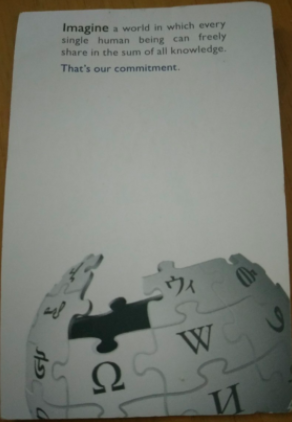
\includegraphics[width=.4\textwidth]{Images/cartao_wmf.png}
    \caption{Verso do cartão de visitas dos funcionários da Wikimedia Foundation.}
    \label{fig:cartao_wmf}
\end{figure}



\newpage

\section{A realidade confunde}

\singlespacing
\begin{flushright}
\textit{``Eu só voltei}

\textit{Pra te contar}

\textit{Viajei}

\textit{Fui pra Serra do luar}

\textit{Eu mergulhei}

\textit{Ah, eu quis voar}

\textit{Agora vem}

\textit{Vem pra terra descansar''}

Walter Franco

\end{flushright}
\doublespacing

\subsection{Para onde vai um conteúdo reprovado?}

\textbf{Cena 3, Abril de 2017.\footnote{Cena escrita a partir de entrevista realizada com Alberto Lima no Rio de Janeiro, no dia 06 de fevereiro de 2020. Quando não explicitamente atribuídas a outrem, todas as aspas desta sessão são falas do entrevistado.} Rio de Janeiro.}

O engenheiro Alberto Lima, professor do curso técnico em Eletrônica do CEFET/RJ, liga seu computador decidido a criar o verbete ``Andes-SN'' na Wikipédia, para falar sobre o Sindicato Nacional dos Docentes das Instituições de Ensino Superior.

Concursado em 2011, Alberto participou ativamente do movimento grevista de 2012, greve esta deflagrada pelas bases em assembleia, contrariando indicação das direções sindicais. Após integrar o comando local de greve, inclusive participando de grandes atos em Brasília/DF, Alberto se junta a companheiros/as paredistas em 2013, concorre, e ganha a eleição para a direção da Adcefet-rj, seção sindical do Andes em sua instituição.

Ao final de sua gestão como presidente do sindicato local, em 2017, Alberto acreditava que o Andes-SN, apesar de ser um dos maiores sindicatos do Brasil, com seções em todas as universidades federais, não possuía uma grande presença digital. Resolveu ler sobre boas práticas de criação de verbetes na Wikipédia e, apesar da dica encontrada de começar editando artigos pré-existentes ao invés de criar um novo do zero, sentiu-se preparado para criar um verbete. Pesquisou se existiam artigos sobre outras entidades similares à sua, e se lembra de ter encontrado vários, ``\textit{alguns inclusive bem curtos com apenas uma referência}''. Com sua pesquisa feita, sentiu-se confiante e começou a escrever sobre seu sindicato nacional.

O professor nos conta que começou a escrever direto na página da Wikipédia. Fez um texto longo, ``\textit{que tinha inclusive uma ligação interna}'', duas referências e estruturado com ``\textit{Introdução} e "\textit{contextualização}''. Se sentia seguro e confortável ao escrever alí, pois afinal ``\textit{qualquer um pode editar a Wikipédia}''.
	
Sabia que seu texto ``\textit{não estava completamente redondo}'', mas resolveu salvar como estava para continuar mais tarde. Nosso editor novato nos conta que já tinha visto alguns verbetes na Wikipédia marcados com avisos como ``\textit{esboços}'', ``\textit{demandando estruturação}'' ou ``\textit{carece de referências}'', e sabia que a mesma coisa poderia acontecer com seu verbete, que seria melhorado mais tarde.

Porém, alguns segundos depois ele é surpreendido por uma notificação informando que seu artigo havia sido removido pelo administrador EVinente, atendendo a um pedido de outro usuário. Ao acessar o endereço da página, se deparou com a seguinte imagem:

\begin{figure}[H]
    \centering
    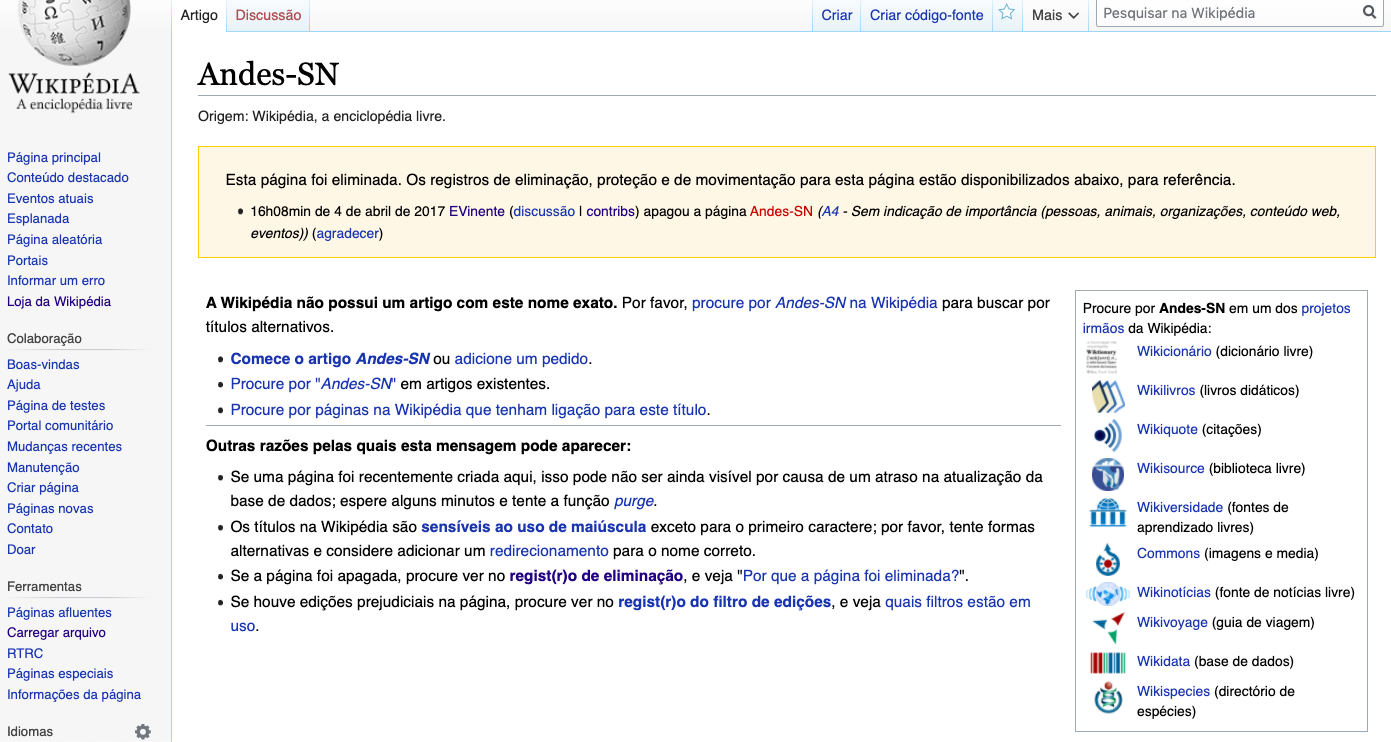
\includegraphics[width=1\textwidth]{Images/andes.png}
    \caption{Verbete Andes-SN com aviso de eliminação.}
    \label{fig:verbete_andes}
\end{figure}

Lembrando das apresentações assistidas nos seminários de pesquisa sobre controvérsias na Wikipédia, Alberto vai à página de discussão do usuário que solicitou a eliminação, onde o profesor então explica saber que o verbete ainda não estava ideal, que teria mais referências para adicionar (``\textit{notícia de greve é o que mais tem}''), inclusive com uma tese acadêmica sobre a história do sindicato. Concluiu informando que gostaria de continuar editando.

\begin{figure}[H]
    \centering
    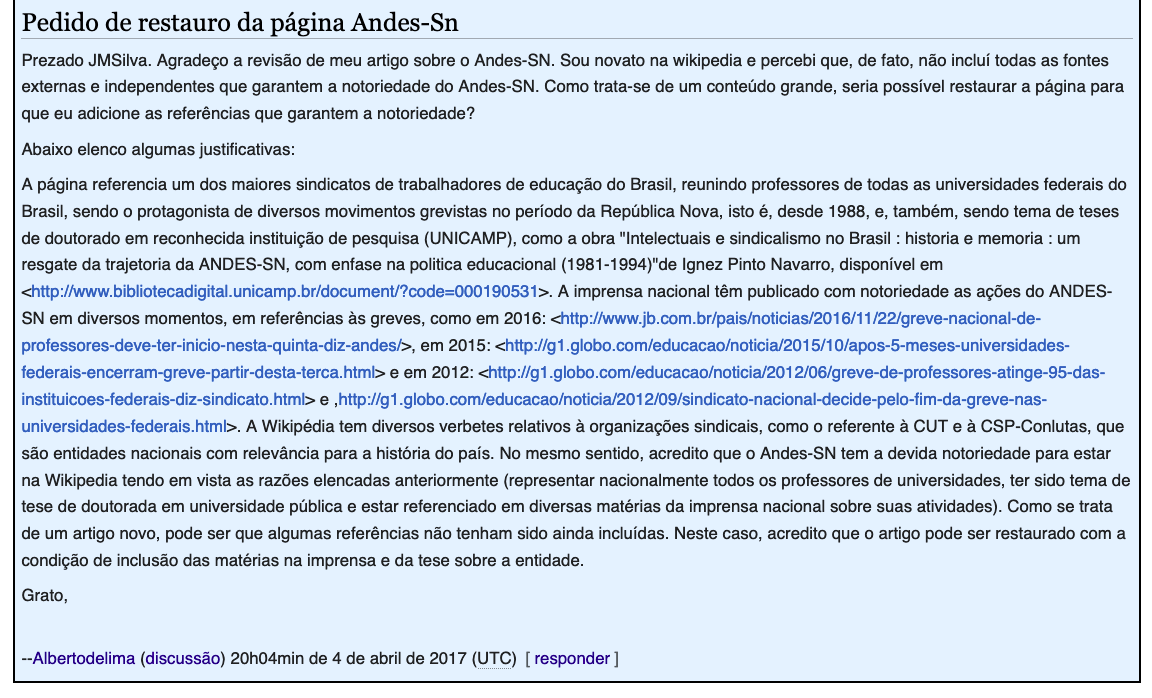
\includegraphics[width=1\textwidth]{Images/alberto-pedido-restauro.png}
    \caption{Página "Wikipédia:Pedidos/Restauro" com o pedido de Albertodelima para que a solicitação remoção feita por JMSilva fosse revista.}
    \label{fig:pedido_restauro_andes}
\end{figure}


O Diálogo então, segundo a memória de nosso protagonista, seguiu mais ou menos assim:

-Se você já sabia onde encontrar mais referências por que não as colocou logo?

-Eu estava sem tempo, mas vou colocar. Porém, o que eu já escrevi sumiu. Quero editar e melhorar, mas não tenho backup.

- Você vai ter que escrever tudo de novo.

Alberto, traído pela confiança na ferramenta, não seguiu sua prática corriqueira de escrever offline e depois "copiar e colar" o conteúdo criado em uma ferramenta online, e agora se via sem possibilidade de acessar novamente sua criação, eliminada do histórico público da Wikipédia.
Como resultado, ele, que estava ocupado com a reta final de seu mandato à frente da Adcefet-rj e já cursando doutorado, resolveu abrir mão de disputar a construção de conteúdos na Wikipédia. ``\textit{Eu nunca mais criei nenhum outro artigo. Nem esse.}''

No início de 2020, Alberto ficou feliz em ver que fora criado em 2018 outro verbete sobre o Andes-SN, desta vez levando seu nome completo, ``Sindicato Nacional dos Docentes das Instituições de Ensino Superior''. Apesar do novo verbete ser muito inspirado na seção ``Sobre'' da página sindicato, não apresentar nenhuma referência, ser muito menos acadêmico que o anterior, e de ter recebido as marcações de ``\textit{Este artigo não cita fontes confiáveis e independentes}'' e ``\textit{Este artigo é um esboço}'', em nenhum momento foi ``proposto para eliminação''.
\newpage
\subsection{Engajamentos e desengajamentos}

\textbf{Cena 4, Janeiro de 2016. Niterói, Brasil.\footnote{Cena escrita a partir de entrevista realizada com Carlos Eduardo Mattos da Cruz no Rio de Janeiro, no dia 06 de fevereiro de 2020. Quando não explicitamente atribuídas a outrem, todas as aspas desta sessão são falas do entrevistado.}}

Carlos Eduardo Mattos da Cruz, responsável pela criação de cursos para os telecentros do município\footnote{Espaços criados para o desenvolvimento de atividades educacionais complementares pelo Programa Niterói Digital, desenvolvido pela Secretaria Municipal de Educação, Ciência e Tecnologia de Niterói.}, orgulhosamente recebe o coordenador do Wiki Educação Brasil, grupo local reconhecido pela Wikimedia Foundation, para iniciar o curso de capacitação de professores/as da rede municipal no uso dos projetos Wikimedia, seguindo a proposta dos telecentros de oferecer uma ``\textit{educação contemporânea sem a ditadura do MEC}''.

O projeto desta formação foi desenvolvido por Cadunico, como Carlos gosta de se apresentar, a partir de conversas com funcionários da Wikimedia Foundation, que contaram-lhe sobre como os projetos educacionais com a enciclopédia só aconteciam em universidades, e que havia o desejo de diversificar o perfil dos editores e levar a prática de escrita wiki para outros níveis educacionais.

Cadunico decidiu tocar o projeto mesmo tendo experiências pessoais não agradáveis no mundo das wikis. Em julho de 2012, criara um verbete sobre o Gnugraf, maior evento de softwares livres para edição gráfica da América Latina, organizado por ele e por sua esposa Cléo Mattos. Pouco tempo depois, foi surpreendido com a remoção do verbete. Através do apoio de amigos que trabalhavam para o movimento e de um editor experiente, conseguiu, ``\textit{depois de muito sufoco}'', deixar no ar uma versão bem simplória do texto original. Até hoje Cadunico tem receio de editar o verbete e adicionar mais informações, para não ``\textit{chamar a atenção}'' de revisores, que podem novamente decidir apagá-lo, assim como aconteceu com sua página de usuário.

Foi em maio de 2013 que ele teve sua página de usuário apagada na Wikipédia. Em suas palavras, ``\textit{porque coloquei mais um item em uma lista de coisas que eu já tinha feito e um robô bloqueou a página}''. Curiosamente, ao observarmos o histórico da página, vemos que a ação não havia sido realizada por um robô, e sim por um dos usuários humanos mais ativos da Wikipédia lusófona. Perguntado sobre mensagens recebidas em sua página de discussão, Cadunico disse desconhecer tal ferramenta, e emendou: ``\textit{quando entro no Facebook pela primeira vez ele tem umas setinhas e umas formas de mostrar onde estão as coisas. Não me lembro de ter visto isso quando me cadastrei na Wikipédia. Só utilizei a 'caixa de areia'\footnote{Área da Wikipédia onde editores podem realizar testes.} por que eu já tinha conversado com pessoal da fundação que me falou dela. Mas ainda assim, a gente escreve lá e ninguém lê. Ninguém te dá dicas sobre o que melhorar antes de enviar conteúdo para o artigo}''.

Após frustrar-se com a Wikipédia, Cadunico ``se muda'' para o Wikilivros, projeto do Movimento Wikimedia para escrita de livros didáticos. Consegue com sucesso criar uma apostila para utilização do software de diagramação \textit{Scribus}\footnote{Apostila disponível em  https://pt.wikibooks.org/wiki/Apostila\_de\_Scribus , acessada em 30 de março de 2020.}, retomando assim sua confiança na possibilidade de trabalhar em conjunto com o movimento.

Então, em 2015, Caudnico convidou representantes do Movimento Wikimedia, que trabalhavam em conjunto com a Fundação, para serem responsáveis pela formação dos/as professores/as. Acreditou que essa chancela evitaria que situações desagradáveis como as vividas por ele na Wikipédia se repetissem. ``\textit{Eu queria botar nos telecentros o símbolo da Wikimedia, e falar que aqui é um núcleo oficial, com aula dada pelo pessoal da própria Fundação. Fizemos banners e tudo mais}''.

A meta do projeto era fazer com que professores da rede municipal de Niterói adotassem ferramentas wiki em suas práticas pedagógicas. A ideia era o/a professor/a editar em suas horas fora de sala de aula, bem como editar com seus/suas alunos/as. Para além da Wikipédia, eles/elas seriam estimulados a escrever livros didáticos em conjunto no Wikilivros e inclusive a compartilhar seus planos de aula no Wikiversidade. O projeto ainda previa, em um segundo momento, expandir a capacitação para a Secretaria de Turismo, que poderia ajudar a manter verbetes na Wikipédia sobre a cidade de Niterói.

O projeto era grandioso. Contaria com ciclos de dois anos, com um ano de capacitação seguido de um ano com os/as professores/as atuando de forma independente, e no ano seguinte um novo ciclo se iniciaria, com nova formação para reciclagem e aprofundamento. Os encontros aconteciam no Telecentro do Terminal Rodoviário João Goulart. ``\textit{Era o maior telecentro, com a melhor internet e as melhores máquinas}''. Por duas vezes na semana, a equipe de lá parava de atender os outros telecentros (o escritório de gestão de todos os telecentros do município ficava nesta unidade e sua equipe auxiliava no suporte aos telecentros menores) para se dedicar exclusivamente à capacitação Wikimedia.

``\textit{Treinamentos como este começam cheios e terminam vazios. Mas com este foi diferente. Começou cheio e terminou mais cheio ainda.}'' O boca a boca entre os/as professores/as era intenso. Todo dia um/a professor/a ligava perguntando se ainda tinha vaga, e a política da Secretaria de Educação era sempre falar que tinha, para depois se virar em acomodar todo mundo. Um dia Cadunico foi convocado pelo secretário de educação, que queria monitorar o maior problema das capacitações ofertadas no município:

- E aí, como está a evasão?

- Não teve evasão.

- Que bom, então todos os alunos que começaram terminaram?

- Mais ou menos.

- Não estou entendendo.

- Começamos com um aluno por micro, e terminamos com três.

Após um ano de treinamento, era chegado o momento dos/as professores/as criarem conteúdos sem apoio de instrutores experientes. Se aproveitando de práticas de acompanhamento da aplicação dos conteúdos dos cursos com feedback contínuo dos professores, desenvolvidas no projeto "Academia de Jogos", que ensinava a criação de softwares educacionais para crianças e professores, a Secretaria de Educação seguiria então ao longo do ano monitorando de perto a fase do projeto de edição nas wikis.

``\textit{Aconteceu com eles o que aconteceu comigo}'', conta Cadunico. ``\textit{Não era a grande maioria. \textbf{Todos estavam frustrados}. Os professores não conseguiam ter o gosto de ver seus conteúdos publicados}''. Cadunico acrescenta que um professor de história da escola municipal do Fonseca, autor de uma tese acadêmica sobre Niterói antiga, e o mais empolgado durante a capacitação, ``\textit{foi sumariamente censurado e desistiu}''.

E não foram só os professores. Novamente Cadunico se sentiu censurado pelo movimento que ele tanto admirava por ter ``\textit{a missão mais nobre do planeta: a de disponibilizar livre e gratuitamente todo o conhecimento humano}''. Enquanto os professores trabalhavam com as wikis, Cadunico resolveu começar um livro didático no Wikilivros. Um livro de pensamentos que, assim como sua página na Wikipédia, foi apagado. A justificava dada para o apagamento sentensiava que seu material não era considerado um livro didático, sem que Cadunico tivesse recebido qualquer aviso, tentativa de diálogo ou chance de defesa. ``\textit{Um livro de pensamentos não é um livro didático para ensino de português ou literatura? Isso é uma forma de censura. Não deixam explícito que tipo de livro é aceitável ou não, o que já acho errado pois para mim todo livro é aceitável, e simplesmente arrancam seu trabalho, de forma impessoal e muito fria.}''

Independente das frustrações, o projeto seguia o cronograma planejado. Depois de passado meio ano de atividades de escrita wiki sem acompanhamento dos especialistas wikipedistas, a secretaria avisou aos/às professores/as que no início do ano seguinte começaria uma nova turma do projeto, buscando levantar a demanda para realizar seu planejamento. Vários/as professores/as pediram para não acontecer uma próxima versão, solicitando que a secretaria criasse outro projeto, pois eles/as estariam sendo censurados/as e maltratados/as na Wikipédia. ``\textit{Tínhamos conseguido um pequeno exército para editar conteúdos brasileiros, e ele foi se desmotivando e se dissolvendo}''. Perante tantos retornos negativos e nenhum caso de sucesso, o projeto foi cancelado e o segundo ciclo nunca se inicio.

Em paralelo, os telecentros promovíam capacitações de LibreOffice, em parceria com Eliane Domingos e Oliver Hallot, da Associação Libre de Técnicas Abertas (ALTA), parceira local da The Document Foundation\footnote{Organização mantenedora do software LibreOffice.}. Estas capacitações, que formaram mais de 30 mil pessoas, tiveram como contrapartida da equipe de Niterói o compromisso de manter a wiki com a documentação do LibreOffice em português atualizada. ``\textit{O que foi fácil, pois os professores já haviam aprendido a utilizar o MediaWiki nos cursos da Wikimedia}''.

Os/as professores/as de inglês acompanhavam a lista de e-mails dos/as desenvolvedores/as do LibreOffice e passavam para colegas as necessidades de atualização da wiki. A versão em português da documentação era atualizada em tempo real, muitas vezes mais rápido que em inglês. Neste projeto a equipe ficou muito motivada, com professores/as editando inclusive em suas horas vagas, relatando se sentirem úteis e valorizados/as. ``\textit{No LibreOffice ninguém os revertia. Provando que o problema nos projetos Wikimedia não eram ocasionados por falta de qualidade de nossa equipe.}'' \citep{cadunico_2020}
\newpage
\subsection{Comunidade local decisões globais }

\textbf{Cena 5. Junho de 2017. Rio de Janeiro, RJ.}

A disciplina ``Estudos CTS (Ciências-Tecnologias-Sociedades): aproximações brasileiras e latino-americanas'' é ministrada no Programa de Engenharia de Sistemas e Computação da COPPE/UFRJ no 2º período de 2017. A turma é convidada a ler o capítulo 7 do livro ``\textit{Yes, nós temos Pasteur. Manguinhos, Oswaldo Cruz e a história da ciência no Brasil}'' \citep{cukierman_pasteur_2007}, intitulado ``\textit{Prata Preta}''.

``\textit{Chamava-se Horácio José da Silva, mas, que importava?}'' \citep[p. 220]{cukierman_pasteur_2007}. A frase que abre o capítulo citado se refere ao Prata Preta, um personagem da Revolta da Vacina ocorrida no Rio de Janeiro, em 1904, que, como tantos outros tipos, não é encontrado nas narrativas universalizantes da história da ciência brasileira. A leitura, que narra momentos decisivos para a construção sociotécnica das ciências brasileiras pelo ângulo de um personagem que não pensaríamos \textit{a priori} como protagonista, provoca algumas reflexões: a quantos outros/as anônimos/as da história da ciência e tecnologia brasileiras a frase de abertura poderia se referir? Como se faz educação em ciências contextualizada em um país com tantos/as atores/atrizes sem voz? Em espaços populares, fora das salas de aulas dos programas de pós-graduação, quais histórias são contadas e quais versões são aprendidas?

Após a leitura, com todas essas perguntas na cabeça, recebo uma provocação de meu colega de pós-graduação, o doutorando Fernando Severo: ``\textit{vamos melhorar o verbete sobre o Prata Preta na Wikipédia?}''. Imediatamente aceito o convite e vamos analisar o material já existente na enciclopédia. Percebemos então que o verbete biográfico de Prata Preta possuía apenas 1754 bytes\footnote{Unidade de medida utilizada pela comunidade Wikimedia para medir o tamanho de revisões e verbetes.}, sendo a metade deles sobre um bloco de carnaval que leva seu nome.

\begin{figure}[H]
    \centering
    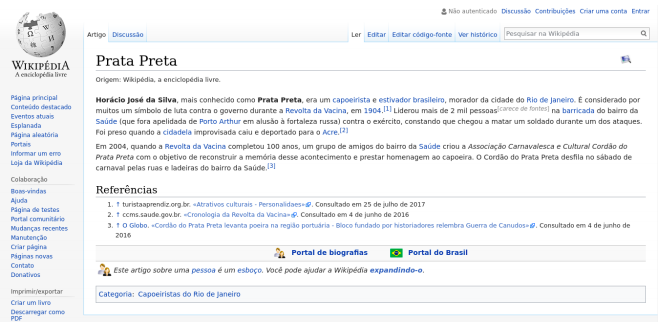
\includegraphics[width=1\textwidth]{Images/pratapreta.png}
    \caption{Versão do verbete Prata Preta encontrado no dia da cena.}
    \label{fig:verbete_pratapreta}
\end{figure}

Aceito o desafio de melhorar o verbete e, enquanto penso sobre os desafios de escrever uma biografia de um subalterno sem voz, com poucas fontes secundárias fiáveis versando sobre sua história, faço uma singela edição com pequenos ajustes ao texto que já estava lá. Para minha grande surpresa, a edição não é salva pela Wikipédia, que me informa: ``\textit{Seu IP está bloqueado}''.

Rapidamente descubro que na verdade não só eu, como milhares de usuários/as da Virtua, maior provedora de internet do Rio de Janeiro, já estavam bloqueados/as por três meses, como resposta a um suposto vandalismo excessivo feito em vários idiomas pelo mesmo range de IP. Essa drástica medida é tomada quando se entende que uma ação orquestrada de vandalismo estará se aproveitando de um provedor de acesso, VPN\footnote{Do inglês Virtual Private Network. São conexões entre máquinas na internet que direcionando o tráfego de uma sempre para a outra.} ou Proxy para mudar de IP constantemente e furar o bloqueio individual a um determinado IP individualizado. E pior, diferente da estratégia de bloqueio simples de IP, onde basta o/a editor/a criar uma conta de usuário/a para (agora rastreado) poder voltar a editar, o bloqueio de faixa de IP incluía também usuários/as registrados/as. Com isso, mesmo meu usuário, com milhares de edições e ficha corrida limpa na enciclopédia, estava proibido de editar.

Fomos então estudar o histórico de edições feitas em nossa faixa de IP e nos surpreendemos com o resultado! Como pode um usuário holandês, que aplicou o bloqueio em todos os sites do Movimento Wikimedia, ter colocado no mesmo balaio de gato Fernando Severo, eu, o IP 179.210.26.120, que estava escrevendo sobre uma escola de samba teresopolitana em português, e o IP 179.210.99.239, que editava sobre a série televisiva ``Meu Pequeno Pônei'' em galego? Não terá seu olhar saxão sido capaz de perceber a distância entre interesses tão distintos e ações de edição? Terá ele conseguido ver apenas uma horda anárquica subdesenvolvida que não tem modos nem educação para escrever uma enciclopédia!?

Saímos então da periferia que é a Wikipédia lusófona e fomos buscar os centros globais de tomada de decisão da enciclopédia. Estudamos as políticas de acesso e de bloqueio globais da comunidade Wikimedia e fomos parar em uma sala de chat em inglês no IRC.\footnote{Do inglês \textit{Internet Relay Chat}, ferramenta para criação de salas de bate papo virtuais.} Lá conversamos com os/as ``gringos/as'', relatando detalhadamente ``o causo'', procurando esclarecê-los a respeito da estrutura do mercado de internet no Rio de Janeiro, com milhões de usuários/as e poucos provedores de acesso; das diversas edições feitas em diferentes wikipédias por editores em nosso range de IP; da forma dinâmica como funciona a distribuição de IP nos provedores de internet; do longo histórico de bom comportamento de meu usuário. Vários/as aliados/as foram convocados/as ao esforço de demonstrar que nosso grupo nada homogêneo, unido involuntariamente por uma faixa de endereços de IP, tem seu valor para a comunidade, e pode ser produtor de conhecimento. Recebi uma desanimadora resposta burocrática de um anglófono, que simplesmente mandou enviar e-mail para um determinado endereço e esperar por um resposta sem prazo.

Mas, eis que de onde parecia que não surgiria mais alento, emerge a empatia de um \textit{steward}\footnote{No Movimento Wikimedia são usuários com permissões para administrar todas as wikis de todos os projetos.} falando português. Ele se solidariza com nosso pleito e nos autoriza a participar novamente do jogo global de construção de conhecimentos na wiki universal, relaxando parcialmente o bloqueio. Agora, após nossa expedição exploratória da implementação da política de bloqueios globais do Movimento durar toda a madrugada, poderíamos novamente editar, desde que estivéssemos devidamente registrados no site com um usuário próprio. Usuários/as anônimos/as continuariam impedidos/as de editar. Afinal, nosso pleito ``tinha seu valor sim, mas também não era para tanto, né?''. Com a confirmação de que havíamos conseguido superar a pane, compondo um novo arranjo suficiente para estabilizar o funcionamento da Wikipédia para nossos usuários, fomos dormir às 5 horas da manhã, sem realizar nenhuma edição no verbete de Prata Preta.

\section{A pesquisa se materializa}

Abrimos este trabalho com cinco cenas, mas poderiam ter sido apresentadas centenas outras em torno da mesma temática. Cotidianamente a Wikipédia convive com esta dicotomia entre ser aclamada como o maior projeto de produção compartilhada de conhecimento da história da humanidade, onde ``todos podem editar'' e ser acusada de não estar aberta para receber colaborações que não estejam perfeitamente enquadradas em um determinado padrão.

São incontáveis os casos de pessoas que, mesmo familiarizadas com movimentos de cultura livre e com dinâmicas educacionais, como os/as personagens de nossas cenas, ao se aventurarem no mundo onde ``qualquer um pode editar'' encontram barreiras relacionadas a ``o que pode ser editado''. Ao mesmo tempo, wikipedistas que propagam o discurso de que ``qualquer pode editar'', e se orgulham desta abertura de seu projeto, parecem não enxergar estas barreiras, que para editores/as experientes teriam soluções óbvias.

O constante convívio do autor desta dissertação com estas cenas antagônicas motivaram e deram o tom desta pesquisa, que passa a ter seus escopo e metodologia apresentados no capítulo a seguir.
%capítulo 2: mantendo a mente quieta
%\chapter{Mantendo a mente quieta}

\singlespacing
\begin{flushright}

\textit{``Tudo é uma questão de manter}

\textit{A mente quieta}

\textit{A espinha ereta}

\textit{E o coração tranquilo''}

Walter Franco

\end{flushright}
\doublespacing

\subsection{Todos/as podem editar?}

Todos/as podem editar a Wikipédia, mas a tarefa não é tão fácil quanto pode parecer. É amplamente documentada a dificuldade de entrada de novos/as editores/as \citep{antin_my_2011}; \citep{burke_feed_2009}; \citep{faulkner_etiquette_2012}; \citep{halfaker_rise_2013}; \citep{kraut_dealing_2010}; \citep{morgan_tea_2013}; \citep{schneider_accept_2014}; \citep{steinmacher_social_2015}. Existem várias regras que dizem o que pode ou não ser escrito, e muitas delas já estão naturalizadas nas ações cotidianas dos/as usuários/as experientes e também nos softwares que gerenciam e atuam na enciclopédia.

Este trabalho pretende pesquisar a aplicação destas regras, entendendo seu histórico de criação, seu processo de naturalização e os efeitos que causam nos/as novatos/as que são pegos/as de surpresa ao tentar editar, e não tem ideia de todo o complexo mundo de governança da enciclopédia.

A Wikipédia é o décimo site mais acessado do mundo, e o décimo-quinto do Brasil. Em ambos os rankings é o site mais visitado mantido por uma instituição sem fins lucrativos \citep{alexa_2019}. No ano de 2019, apresentou uma média de 500 milhões de visitantes únicos por mês \citep{wikimedia_stats_2019}. Os imponentes números de sua audiência dizem que uma informação que perdure na Wikipédia tenderá a ser lida por milhares de pessoas e replicada indefinidamente, o que nos mostra a grande relevância desta ferramenta no mundo contemporâneo e sua centralidade na construção de fatos em nosso tempo.

Todos esses acessos estão distribuídos entre mais de 40 milhões de verbetes escritos em diferentes 303 idiomas, que atualmente são mantidos por aproximadamente 400 mil editores/as ativos/as \citep{wikimedia_stats_2019}. No momento, a versão lusófona conta com um pouco mais de um milhão de verbetes, mantidos por aproximadamente 3600 usuários/as ativos/as \citep{wikimedia_stats_2020}\footnote{Dados encontrados em https://stats.wikimedia.org/\#/pt.wikipedia.org/contributing/active-editors/normal|line|2-year|~total|monthly , acessada em 12/02/2020.}. É inquestionável que seus números de editores são grandiosos, e a um primeiro olhar esse volume pode parecer sustentar a afirmação de que afinal "\textit{qualquer um/a pode editar}".

A primeira cena apresentada versa sobre Jimmy Wales, um dos fundadores da Wikipédia e diretor executivo da Wikimedia Foundation até 2007. Ao contrário do que se poderia achar, sua saída da fundação, há mais de uma década, não fez desaparecer o discurso aqui posto à prova pelas cenas. Sua sucessora, Sue Gardner, manteve a linha do discurso, como pode ser visto em diversas falas\footnote{Publicação feita em seu blog pessoal acessada em 12/02/2020. https://suegardner.org/2013/01/14/the-people-behind-wikipedia-the-encyclopedia-anyone-can-edit/ .}, palestras\footnote{Palestra apresentada em 2010 e acessada em 12/02/2020 https://www.youtube.com/watch?v=vzJCHQ42XAw\&t=127s .} e entrevistas\footnote{Entrevista concedida em 2013 e acessada em 12/02/2020 https://www.youtube.com/watch?v=Y6gYhHWglBA .} concedidas ao longo dos 8 anos de sua gestão. Gestão marcada pela construção de programas que buscaram estimular a contribuição editorial de grupos sociais sub representados dentre os/as editores/as da enciclopédia, tais como moradores/as do sul global e mulheres, levantando uma bandeira que podemos tentar resumir em "todos/as devem ter condições de editar"\footnote{Esse discurso pode ser encontrado em diversos materiais, tais como esta entrevista dada em 2012 e acessada em 12/02/2020 https://www.youtube.com/watch?v=UoWgqPcF-TQ .}, mas sem jamais abandonar o "qualquer um/a pode editar".

A expressão "qualquer um/a pode editar a Wikipédia"\footnote{A expressão utilizada no buscador foi exatamente: "qualquer um pode editar" Wikipédia} é tão onipresente em discursos de \textit{hackers}, militantes da cultura livre, professores/as e até mesmo de seus/suas críticos/as que, uma rápida busca por ela no Google, retorna mais de 18 mil resultados. Indo além, ao testarmos a versão original da afirmação em inglês “\textit{anyone can edit Wikipedia}”\footnote{A expressão utilizada no buscador foi exatamente: "anyone can edit" Wikipedia}, a maior ferramenta de buscas do mercado retornou mais de 660 mil links\footnote{Buscas realizadas no endereço www.google.com em 28/01/2020.}.

Fazendo um recorte apenas por trabalhos acadêmicos, utilizando a ferramenta Google Scholar\footnote{Busca realizada no serviço https://scholar.google.com em 28/01/2020.}, nos foram apresentados mais de 3 mil trabalhos com o referido termo em inglês. Esse enorme volume sustenta que nossa cena inaugural não está descolada da realidade, e reforça a popularidade do termo, inclusive dentre os/as estudiosos/as da enciclopédia virtual.

É importante notar que o discurso está presente tanto na fala dos/as defensores/as do modelo distribuído da enciclopédia como na de seus/suas críticos/as. O que para alguns é visto como um diferencial competitivo, para outros é um problema irreparável. Não é difícil encontrar tanto falas de intelectuais como expressões da cultura popular do mundo digital contemporâneo, através dos memes\footnote{Diversos exemplos de memes podem ser encontrados em buscas como https://www.google.com/search?q=meme+wikipedia+anyone+can+edit\&tbm=isch. Nos exemplos aqui exibidos na figura \ref{fig:memes}, a primeira imagem está escrito sobre a vítima ``Usando Wikipédia como fonte'' e sobre o atirador ``Mas qualquer um pode editar''. Segunda imagem: acima da professora está escrito ``Você não pode utilizar a Wikipédia como fonte'', e abaixo "qualquer um pode editar".}, atacando a Wikipédia exatamente por qualquer um poder editá-la. A própria Wikipédia mantém um verbete chamado ``Críticas à Wikipédia'', e dos seus 39 tópicos, o primeiro a ser apresentado é não por acaso chamado ``Crítica ao conteúdo'', que apresenta um texto de Robert McHenry, editor da Encyclopædia Britannica, afirmando não ser possível existir a fiabilidade enciclopédica em uma obra editável abertamente. \citewiki{ptwiki_criticas}\footnote{Sempre que uma página de uma Wikipédia for citada durante o estudo ela será referenciada seguindo o padrão: (``idioma'', ``nome da página'', ``data da edição'').}

\begin{figure}[H]
    \centering
    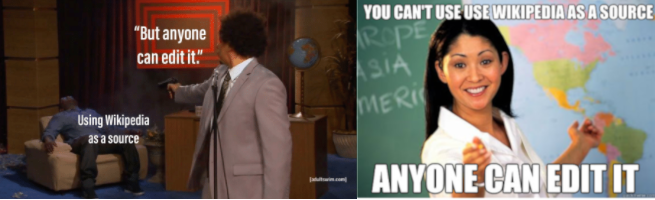
\includegraphics[width=1\textwidth]{Images/memes.png}
    \caption{Exemplos de memes sobre a Wikipédia.}
    \label{fig:memes}
\end{figure}

Os questionamentos de críticos relacionados a impossibilidade de se manter uma enciclopédia de qualidade que "qualquer um/a possa editar" são recorrentemente explorados e discutidos por professores/as, conteudistas, jornalistas e pesquisadores/as. Nestes questionamentos diversos fatores são colocados em xeque, mas invariavelmente todos assumem como verdade a afirmação de que "qualquer um/a pode editar". Não encontramos na literatura esforços para testar esta assertiva, esmiuçando o discurso propagado por todos os lados, sustentado em seus grandiosos números globais e na estrutura de uma ferramenta wiki aberta e colaborativa.

Assim, iremos nas próximas seções iniciar esforços de verificação na prática cotidiana, na vida real dos ``qualquer uns/umas'', a consistência deste discurso.

\subsection{O autor desta dissertação pode editar?}

\singlespacing
\begin{flushright}

\textit{``Tudo é uma questão de manter}

\textit{A mente quieta}

\textit{A espinha ereta}

\textit{E o coração tranquilo''}

Walter Franco

\end{flushright}
\doublespacing

Para proporcionar ao leitor uma apreciação situada deste trabalho, entendo ser importante explicitar aqui minha trajetória com a Wikipédia e sua comunidade. Sou militante do movimento software livre desde 2003, participando de diversas comunidades reunidas em torno de causas ligadas ao que chamamos de cultura livre, tanto a do desenvolvimento de software como a da evangelização de novos/as entrantes. Dentro destes movimentos, sempre foi corriqueira a prática de utilizar ferramentas wiki para documentar nossas atividades e construir \textit{sites} de forma colaborativa.\footnote{O TWiki, sistema mais popular de gestão de wikis do início do século teve sua primeira versão lançada em 1998 REFERÊNCIA: https://twiki.org/ .}

Em meados da década 2000 conheci a Wikipédia e, já habituado a ferramentas wiki, passei instintivamente a realizar edições pontuais como usuário anônimo. Em toda minha experiência com wikis, apenas tive usuário registrado naquelas em que a edição era restrita a cadastrados, pois não via sentido em criar uma conta em uma wiki que qualquer um poderia editar.

No dia 27 de Fevereiro de 2009 passei por uma surpresa. Ao acessar o site da Wikipédia vi em destaque no topo da página "\textit{Você tem uma mensagem nova}", e tive certeza de que se tratava de um bug da plataforma. Afinal, eu não estava logado, então não seria possível me enviarem mensagens. Decidido a investigar o bug cliquei no link, e, para meu espanto, a mensagem realmente era sobre uma edição feita por mim! Neste momento aprendi duas coisas: que a Wikipédia trata seus usuários anônimos pelo IP de conexão\footnote{Essa caraterística do MediaWiki será densamente explorada mais a frente na pesquisa.}, permitindo, ainda que de forma precária, rastreá-los minimamente; e que é importante ter um usuário cadastrado mesmo em uma wiki em que qualquer um pode editar, pois isso facilita a troca de mensagens com outros/as usuários/as editando o mesmo artigo que eu porventura também esteja editando.

Confesso um pouco de desconforto inicial com essa funcionalidade de mensagens associadas a usuários do MediaWiki. Outras ferramentas gestoras de wikis mais populares da época, como o TWiki e o TikiWiki, forneciam “apenas” páginas de discussão associadas a cada artigo criado, e não aos usuários. Assim, os debates giravam sempre em torno de uma página específica, e não existia a possibilidade enviar uma "mensagem direta" para um usuário. De cara imaginei que essa funcionalidade de mensagem direcionada a um usuário poderia deslocar discussões das páginas onde elas deveriam acontecer com mais visibilidade\footnote{Essa preocupação reaparecerá e será detalhada no capítulo 3.} além de também personificar as contribuições de uma maneira que me parecia não harmônica com a filosofia dos movimentos livres. Mas, como estava pessoalmente disposto a engajar-me com mais comunidades de produção de conteúdos, para além das comunidades de software, e percebendo a crescente importância da Wikipédia, dei o braço a torcer e criei meu usuário.

Desde então, meu usuário HenriqueCrang realizou 3368 edições nas wikis do Movimento Wikimedia, sendo 80\% delas na Wikipédia em português. Destas, 83,2\%, ou 2.182 edições\footnote{Dados de 03 de março de 2020, acessados em https://xtools.wmflabs.org/ec/pt.wikipedia.org/HenriqueCrang .}, foram feitas no chamado “domínio principal” da Wikipédia, que engloba as páginas com os verbetes enciclopédicos\footnote{A separação das Wikipédias em domínios será explicada no próximo capítulo.}.

Através de meu engajamento com redes de cultura livre, e curiosamente não pelas páginas da Wikipédia\footnote{Em alguns momentos da história os/as voluntários/a engajados em \textit{outreach} no Movimento Wikimedia no Brasil não estiveram próximos das atividades na Wikipédia em português. \textit{``Outreach''} é uma palavra em inglês que significa atividades extramuros, de extensão. Utilizaremos o termo em inglês pois a comunidade lusófona de wikipedistas utiliza-o corriqueiramente. Estas dinâmicas e separações serão melhor trabalhadas no capítulo 3.}, tive contato com o Movimento Wikimedia Brasil, que realizava atividades de \textit{outreach} para promoção das wikis, e passei a participar e organizar atividades no Rio de Janeiro. Em 2012, fiquei sabendo que a Wikimedia Foundation planejava abrir um escritório no Brasil\footnote{https://www1.folha.uol.com.br/fsp/tec/34745-wikipedia-abrira-seu-1-escritorio-no-brasil.shtml} e, ao final deste ano, candidatei-me e fui aprovado para trabalhar diretamente para a Fundação como “analista de dados e experimentos”. A ideia de abrir um escritório no Brasil acabou não vingando, mas tivemos uma equipe de quatro pessoas trabalhando no chamado “Programa catalisador do Brasil”, que buscava aumentar o número de editores ativos nos projetos Wikimedia no país, com especial foco na Wikipédia em português\footnote{Paralelamente foram realizados projetos similares na Índia e no MENA (sigla em inglês para Oriente Médio e Norte da África), regiões que foram mapeadas pela Fundação como apresentando uma baixa relação de editores/as\textbf{/}leitores/as, apresentando assim potencial para um rápido engajamento de novos/as voluntários/as.}.

Vale citar aqui que a Wikimedia Foundation tem como hábito criar um/a usuário/a “de trabalho” para seus funcionários, diferente de seu/sua usuário/a como voluntário/a. Como forma de separar o que era atuação da Fundação (que não financia diretamente a produção de conteúdo) e atuação voluntária, os/as funcionários/as que quisessem contribuir com as páginas de conteúdo deveriam fazê-lo com suas contas de voluntário/a, enquanto deveriam utilizar a conta institucional (normalmente com o nome terminado em “(WMF)” facilitando a identificação pela comunidade) para debater atividades nas quais estivesse atuando remuneradamente pela Fundação. Com meu usuário “HAndrade (WMF)” realizei mais 1612 edições, sendo a maioria delas no Meta Wiki e 36\% na Wikipédia em português.\footnote{Dados disponiveis em https://xtools.wmflabs.org/ec/pt.wikipedia.org/HAndrade\%20(WMF) , acessados em 03 de março de 2020.} Destas edições, 11 foram feitas por distração em verbetes, acreditando estar logado com a conta de voluntário.\footnote{É comum funcionários/as da WMF trabalharem com dois navegadores abertos, mantendo em um logada sua conta institucional e no outro sua conta de voluntário.}

Nestes anos em que trabalhei para a Fundação, atuei tanto auxiliando as comunidades lusófonas a desenvolver análises de dados para se conhecerem e testarem hipóteses, como também engajando voluntários/as técnicos/as para o desenvolvimento de ferramentas demandadas pelas comunidades locais. Estive assim imerso nas controvérsias da Wikipédia em português com disponibilidade, intensidade e dedicação muito maiores do que nos tempos de voluntário. Essa vivência me permitiu conhecer densamente o movimento e seus softwares, estruturas de dados, espaços de decisão e dinâmicas de governança. Tal experiência prévia serviu-me como um enorme e valioso mapa para navegar pelos espaços necessários para realizar essa pesquisa, que com certeza não teria sido desenvolvida da mesma maneira por um/a pesquisador/a recém chegado/a ao mundo Wikimedia.

\subsection{Para quem escrevemos?}

O presente estudo busca alcançar dois públicos-alvos de leitores/as. Pretende-se tanto atrair a comunidade de usuários/as engajados/as na governança da Wikipédia, como pessoas comprometidas com a realização de atividades para a atração de novos/as editores/as.

Ao mapear processos de tomada de decisão e expor as decisões automatizadas, tomadas por sistemas como o software MediaWiki e por robôs patrulhadores, este texto oferece para leitores/as wikipedistas experientes a oportunidade de refletir sobre a constatação de que a Wikipédia tem regras duras, muitas vezes nem conhecidas de sua própria comunidade, e que tendem a se naturalizar através de implementações em software e comportamentos precondicionados.

Olhamos para o histórico de tomadas de decisão da comunidade considerando a “\textit{indeterminação do passado, que (...) é a ideia de que o passado depende do presente e de como se reinterpreta hoje o que aconteceu ontem, sendo estas revisões verdadeiros esquemas de (re)organização do mundo}" (\cite[p.23]{feitosa_cidadao_2010}). Assim, sabendo que “\textit{estamos constantemente revisando nosso conhecimento sobre o passado à luz de novos desenvolvimentos do presente}” (\cite[40]{bowker_sorting_2007}), não tomaremos o dito senso comum da comunidade como verdade definitiva e recriaremos histórias com os enredamentos que cruzarem o caminhar da pesquisa.

Com esse movimento, espera-se oferecer aos/às membros/as da comunidade uma leitura que contribua tanto em momentos de criação de novas regras, como em discussões sobre aplicações de normas vigentes e em casos de enquadramentos/transbordamentos de exceções.

Concomitantemente, ao descrever detalhadamente a realização de editatonas, iremos agrupar práticas de organização desses eventos sugeridas pela comunidade global, expor números de resultados e descrever situações de conflito e resoluções, também fazendo desta obra uma possível referência para extensionistas do Movimento Wikimedia, envolvidos/as na organização de atividades de engajamento de editores/as novatos/as.

Também podem ser citados/as como potenciais leitores/as interessados/as nesta dissertação pesquisadores/as da área dos Estudos de Ciências-Tecnologias-Sociedades (CTS)\footnote{Optamos por esta forma de grafia para nos referenciar ao nosso campo de pesquisa, que pode ser encontrado em diferentes variações em outras obras. Latour, ao falar sobre os "\textit{Science Studies}", diz que "Nunca encontrei duas pessoas que estivessem de acordo quando ao significado do campo de estudo chamado "ciência, tecnologia e sociedade"; na verdade, raramente vi alguém que concordasse quanto ao nome ou quanto à própria existência do campo!" (\cite[p.25]{latour_ciencia_1987})}, que nas seguintes páginas encontrarão um estudo de caso que, não só lança mão de metodologias CTS, como também encontra e descreve práticas de produção de conteúdo com algumas similaridades à prática de produção científica, tão estudada por esta area. Ademais, ciente das diversas experiências desagradáveis sofridas por professores/as e pesquisadores/as ao tentarem editar a Wikipédia (são incontáveis os relatos de situações análogas às das cenas que abrem este trabalho), espera-se que este estudo possa demonstrar para leitores/as não-wikipedistas que a Wikipédia não é "gratuitamente cruel" com novatos/as, e que estes/as possam compreender as barreiras encontradas em suas tentativas de edição, e aprendam possibilidades de buscar desvios e composições em suas futuras disputas pela construção de conhecimento em wikis.

\section{Como fizemos?}

O objetivo central desta pesquisa é abrir a caixa-preta do discurso naturalizado de que ``qualquer um pode editar'', e verificar como ele se constrói e se sustenta na materialidade cotidiana da Wikipédia. Utilizamos o termo caixa-preta conforme definido por Bruno Latour (\citeyear[p. 4]{latour_ciencia_1987}), como algo sobre o qual ``\textit{não é preciso saber nada, a não ser o que nela entra e o que dela sai}''. Assim, para abrir esta caixa-preta, não nos bastará apenas olhar para as funcionalidades colaborativas do software e para os grandiosos números de produção de conteúdo. Como Latour, que ao estudar a construção de fatos e artefatos, diz que ``\textit{nossa entrada no mundo da ciência e da tecnologia será pela porta de trás, a da ciência em construção, e não pela entrada mais grandiosa da ciência acabada}'' (\citeyear[p. 6]{latour_ciencia_1987}), analogamente fizemos a mesma entrada com a Wikipédia, nos ocupando de estudar não seus verbetes prontos, mas o funcionamento cotidiano de suas engrenagens de produção desses verbetes. Assim, não estudamos ``\textit{as coisas 'em si', mas as coisas 'entre si'. Mais importante que as coisas 'nelas mesmas', são suas relações, suas associações}'' \cite[p. 13]{feitosa_cidadao_2010}.

O conceito de caixa-preta, como definido por Latour, é um dos elementos centrais dos Estudos de Ciências-Tecnologias-Sociedades (CTS) que suportam esta pesquisa. Originado na cibernética para se referir a sistemas que seriam muito complexos para serem detalhados, o conceito é empregado como uma representação de uma entidade que recebe uma entrada e fornece uma saída, devendo-se assumir que funciona perfeitamente para seu propósito, sendo desnecessário preocupar-se com seu funcionamento. Latour então utiliza este termo para falar de verdades científicas e artefatos tecnológicos que se naturalizam e são aceitos a priori, sem controvérsias. Assim, abrir uma caixa-preta, seria o movimento de entender como os fatos e artefatos foram construídos (\citep[p.31]{latour_ciencia_1987}). É exatamente neste sentido que utilizaremos o termo ao longo da pesquisa.

A tentativa de entender o funcionamento da enciclopédia com o ferramental metodológico dos Estudos CTS, eleito como balizador desta pesquisa, levou a não observá-la como algo estanque, mas como um organismo vivo, em fluxo. Assim, para entender as dinâmicas da comunidade wikipedista, o presente trabalho foi conduzido com duas abordagens complementares: ``de dentro para fora'' e ``de fora para dentro''. A primeira configurada pelos processos de tomada de decisão e naturalização de regras na Wikipédia em português, e a segunda pela chegada de editores/as novatos/as e as barreiras enfrentadas por eles/as.

Em ambas as abordagens de pesquisa anunciadas utilizamos ferramentais tanto de pesquisas qualitativas como quantitativas, acompanhando densamente trilhas de discussões, históricos de decisões e alterações em ferramentas automatizadas com o olhar próximo e míope de uma formiga – trocadilho usado por Latour, dado que a sigla em inglês para Actor-Network Theory (ANT) tem o mesmo nome do inseto -, ao mesmo tempo em que nos ocupamos de observar quantitativamente suas repercussões e implicações em todo o ecossistema da enciclopédia, com o olhar abrangente e amplo de uma águia.

Dando sequência a apresentação do arcabouço metodológico da pesquisa, é lançada mão da Teoria Ator-Rede (TAR), utilizada para tratar dos enredamentos e estabilizações de fatos científicos e artefatos tecnológicos. Sabemos que fatos e artefatos têm sua própria dinâmica de construção (\cite{fleck_genesis_2010}), mas o caso de artigos na Wikipédia se aproxima bastante dessa dinâmica, e os estudos sobre a construção de textos científicos caem como uma luva para estudos de escritas enciclopédicas. Como diz Esteves (\citeyear[p.102]{esteves_as_2014}), “\textit{a Teoria Ator-Rede propôs definir a factualidade de uma alegação não em termos de uma suposta veracidade intrínseca, mas nos termos de sua resistência aos ataques que ela venha a sofrer. A analogia com a Wikipédia é clara. Latour parecia descrever a verificabilidade nessa passagem de Ciência em ação: ‘E a que resiste [a realidade]? Aos testes de força. Se, numa dada situação, nenhum dissidente for capaz de modificar a forma de um novo objeto, então é isso, é realidade, ao menos enquanto os testes de força não forem modificados’ (\citep[p.93]{latour_ciencia_1987})}”. Neste caso, ou seja, uma vez que cessaram provisoriamente as controvérsias, os/as especialistas e os laboratórios não estão imersos nas controvérsias pela escrita da realidade, mas os/as editores/as da enciclopédia assumem o papel de seus porta-vozes e a disputa, apesar de deslocada, segue dinâmicas similares.

Assim como o fazer da ciência, a escrita da Wikipédia também segue um “\textit{caminho muito estranho porque é invisível quando tudo vai bem}” (\citep[p.44]{latour_cogitamus_2010}). Porém, quando existem divergências entre editores/as, suas redes de aliados que sustentam verbetes instáveis tornam-se visíveis, e publicações científicas, relatórios da ONU, notícias de jornais e demais fontes são arregimentadas por wikipedistas para defender uma versão do texto do verbete. A busca por aliados/as mais poderosos/as para reforçar uma posição dá a impressão de se assemelhar ao que ocorre na tecnociência a tal ponto que a seguinte passagem de Latour (\citeyear[p.48]{latour_cogitamus_2010}), sobre a estrutura textual de publicações científicas poderia muito bem ter sido escrita sobre verbetes da Wikipédia: “\textit{a presença ou ausência de referências, citações e notas de rodapé é um sinal tão importante de que o documento é ou não sério que um fato pode ser transformado em ficção ou uma ficção em fato apenas com o acréscimo ou a subtração de referências”}.

Nos moldes de um “A vida da Wikipédia como ela é", esta pesquisa se apoiará sempre que possível em relatos de casos concretos do cotidiano da enciclopédia que demonstrem a não trivialidade de enquadramentos e fronteiras estanques, colocando uma lupa sobre situações de panes, transbordamentos e recomposições. Pois afinal, são nesses momentos em que as caixas-pretas tornam-se nada óbvias. O seu processo de estabilização (ou não), que permitirá a existência de momentos posteriores estáveis de funcionamento, é exatamente o ponto de interesse da pesquisa. Como ensina Feitosa (\citeyear[p.9]{feitosa_cidadao_2010}), "\textit{um fazer ou estudar tecnologia comprometido em evidenciar as decisões tecnopolíticas relevantes para certos coletivos, deve tentar entender e explicar a relação entre artefatos e esses coletivos, ou seja, deve tentar explicar como as coisas ditas técnicas e as demais entidades (humanas e não humanas) se relacionam, com o fim, inclusive, de indicar caminhos a serem seguidos ou evitados no fazer tecnologia}".


Se para todo enquadramento existe um transbordamento (\cite{callon_markets_1998}), é exatamente nas bordas onde se encontra nosso interesse de estudo. Na definição não trivial, maleável e instável de fronteiras, onde cotidianamente narrativas são configuradas e reconfiguradas no ecossistema da enciclopédia. Um exemplo prático que podemos brevemente citar, para ilustrar ao leitor o local de definição de fronteiras que nos interessa, é a controvérsia em torno da política editorial de verificabilidade da Wikipédia lusófona. Ela enuncia que ``\textit{pessoas lendo e editando a enciclopédia podem checar se a informação provém de uma fonte confiável. A Wikipédia não publica pesquisa inédita; todo seu conteúdo é determinado pela informação previamente publicada ao invés de se basear apenas nas opiniões, crenças e experiências de seus editores. Mesmo se você tem certeza de que algo é verdadeiro, isto deve ser verificável através das fontes da informação antes de você adicioná-lo}'' (\citewiki{ptwiki_verificabilidade}).

Mesmo que aparentemente formulada de forma ``clara'' e ``direta'', esta regra tem suas fronteiras de aplicação constantemente movimentadas por seus/suas usuários/as, que disputam incessantemente contornos entre noções de conformidade, bom senso, respeito e qualidade.

No contexto desta disputa foi criado, em 2011, o ensaio ``\textit{Você não precisa citar que o céu é azul}''. Dissertando sobre a política de verificabilidade, afirma que ``\textit{muitos editores não entendem corretamente a política de citação, e veem nela um mecanismo para obrigar, consolidar ou deixar dúvidas sobre um ponto de vista em particular em uma disputa, ao invés de usá-la apenas para validar a informação da Wikipédia. Isto acaba gerando diversas formas de comportamentos desestabilizadores que devem ser evitados}'' (\citewiki{ptwiki_nao_precisa_citar_ceu_azul}).

Logo após criado, o ensaio viu sua página de discussão ser palco de um acalorado debate, com mais de 46 mensagens feitas por 17 diferentes usuários/as, variando de discordâncias enfáticas a apoios ao ensaio ser tornado uma política oficial. As discordâncias ganharam robustez com a publicação de outro ensaio, em 2013, intitulado ``\textit{É preciso citar que o céu é azul}''. Neste novo ensaio, defende-se que ``\textit{alguns editores podem disputar factos\footnote{Os textos da Wikipédia lusófona podem ser escritos em qualquer das diversas versões do português. Optamos por manter a grafia original das passagens transcluídas e não as adaptar para o português brasileiro.} aparentemente simples e óbvios. Até mesmo a afirmação de que ‘o céu é azul’ pode ser questionada porque o céu muito frequentemente tem cores diferentes, e todas as informações prováveis de vir a ser disputadas precisam de fontes}'' (\citewiki{ptwiki_e_preciso_citar_ceu_azul}). O ensaio ainda acrescenta que o verbete ``\textit{Céu}'', desde 2008, apresenta como legenda de sua figura principal o seguinte texto: ``\textit{quando visto de uma certa altitude, como de um avião, o céu varia de cor}'' (\citewiki{ptwiki_ceu_definicao}).

\begin{figure}[H]
    \centering
    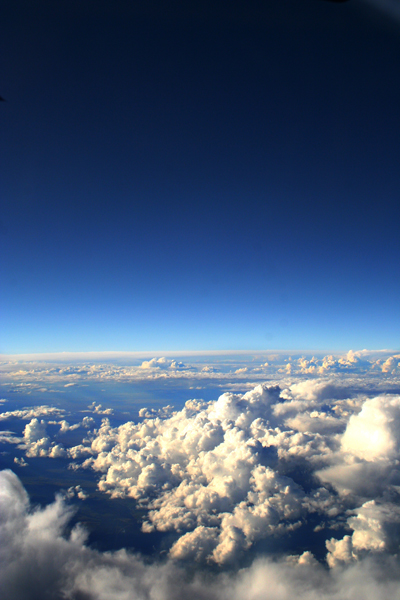
\includegraphics[width=0.4\textwidth]{Images/ceu.png}
    \caption{Imagem que ilustra o verbete “Céu” desde 2008.}
    \label{fig:ceu}
\end{figure}

Seguindo esta linha argumentativa, o ensaio conclui com as seguintes palavras: “\textit{Só porque uma coisa a si lhe parece óbvia, não significa que seja óbvia para toda a gente. Construa artigos unicamente a partir de fontes fiáveis de autoridades no assunto e cite essas fontes}” (\citewiki{ptwiki_e_preciso_citar_ceu_azul}).

Ambos os ensaios estão marcados com a predefinição ``Ensaio contestado'', que anuncia em uma caixa no topo das páginas de ambos ensaios: ``\textit{\textbf{Atenção}: Esta página contém um ensaio da Wikipédia que é seguido por parte dos seus editores, \textbf{mas é contestado por outro grupo de editores}}''\footnote{Grifos do original.} (\citewiki{ptwiki_predifinicoes_ensaios_contestado}). Ou seja, mesmo o primeiro ensaio tendo sido criado em 2011 e o segundo em 2013, até hoje, em 2020, nenhum deles foi reconhecido como uma política oficial da Wikipédia em português, e ambos contam com correligionários/as que convivem na enciclopédia com práticas antagônicas de aplicação da política de verificabilidade.

\begin{figure}[H]
    \centering
    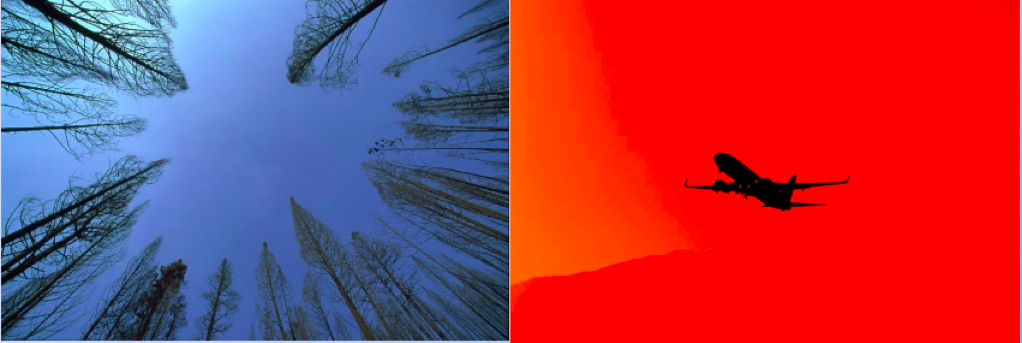
\includegraphics[width=1\textwidth]{Images/ceus-verificabilidade.png}
    \caption{Imagens que ilustram os ensaios que debatem as fronteiras de aplicação da política de verificabilidade.}
    \label{fig:ceus-verificabilidade}
\end{figure}

Situações como a relatada levaram nossa pesquisa a se interessar tanto pelos enredamentos que configuram a governança cotidiana da enciclopédia como pela forma que orientações nada triviais, como a demonstrada, podem se tornar barreiras no caminho de novos usuários que não tenha a experiência requerida para realizar devidos desvios para poderem editar.

A forma como a ambivalência de nossa pesquisa aqui citada se desenvolvera e fora implementada é então detalhada na seção a seguir.

% 
\subsection{Estudos quantitativos e a Wikipédia}

Metodologias quantitativas podem entrar em rota de colisão com os Estudos CTS, pois tendem a realizar inferências que confiam em metadados como fiéis porta-vozes dos fenômenos estudados, assim como tendem a dedicar pouca atenção às traduções\footnote{Utilizamos o termo ``tradução'' da mesma forma que  Bruno Latour, apoiados no conceito criado por Michel Serres em ``\textit{La traduction}'', de 1974, e retrabalhado em ``\textit{Le tiers-instruit}'', de 1991.}, traições, enquadramentos e transbordamentos que estão necessariamente envolvidos no processo de criação de camadas de conhecimento. Como proposto por Henrique Cukierman, em palestra no evento ``Avaliação da produção científica brasileira: pensando com a história das ciências'', organizado em 2011 pela SBHC e pelo HCTE\footnote{Sociedade Brasileira de História da Ciência (SBHC) e Programa de Pós-Graduação em História das Ciências e das Técnicas e Epistemologia da Universidade Federal do Rio de Janeiro (HCTE).}, sobre a confiança nos números, geralmente traduzida como ``objetividade'': ``\textit{O que há de especial com a linguagem da quantidade? Respondendo de forma sucinta, pode-se dizer que a quantificação é uma tecnologia de controle a distância, pouco ou nada relacionada com a chamada 'verdade' da natureza}'' (\cite[p.5]{cukierman_uma_2011}). Em seguida, citando Theodore M. Porter, ressaltou que ``\textit{a quantificação é parte de uma estratégia de intervenção, e não de mera descrição}'' (\cite[43]{porter_1996}, apud \cite[p.5]{cukierman_uma_2011}).

Na literatura de estudos sobre controvérsias na Wikipédia é comum encontrar pesquisadores/as caindo nesta armadilha da autoproclamada "objetividade" dos dados, realizando estudos profundos unicamente alicerçados em metadados que são assumidos como verdades puras e neutras, sem que os/as pesquisadores/as se ocupem em compreender como são elaborados, em observar quais ações foram de fato realizadas pelos/as usuário/as que viriam a gerar tais metadados estudados. É o caso sintetizado por Latour (\citeyear{latour_ciencia_1987}) como "\textit{o representante sendo assumido automaticamente como o representado}". 

Sigamos então com uma breve revisão bibliográfica para observar a materialidade desta prática de utilização dos metadados como porta vozes suficientes nos estudos mais citados sobre controvérsias na Wikipédia.

Em um trabalho bastante citado\footnote{89 citações segundo o Google Scholar. Página disponível em https://scholar.google.com.br/scholar?hl=pt-BR\&as\_sdt=0\%2C5\&q=Edit+wars+in+Wikipedia\&btnG= , acessada em 25 de março de 2020.}, “\textit{Edit wars in Wikipedia}”, Sumi et al (2011) propõem o índice M de controvérsia, observando “\textit{como' o número de edições e reversões desviam em algumas páginas dos números seguidos pela maioria dos artigos}”\footnote{Todas as citações desta revisão bibliográfica foram traduzidas livremente pelo autor.}. Mapeando duplas de editores/as que se revertem em um artigo e seu volume de edições no mesmo texto, os autores testam seu modelo em 6 diferentes idiomas e observam que menos de 1\% dos artigos apresentam um resultado significativo em seu índice.

O trabalho anterior foi a base do estudo ``\textit{The most controversial topics in Wikipedia: A multilingual and geographical analysis}'' de Yaseri e aliados, citado já 100 vezes por outros estudos.\footnote{https://scholar.google.com.br/scholar?hl=pt-BR\&as\_sdt=0\%2C5\&q=The+most+controversial+topics+in+Wikipedia\%3A+A+multilingual+and+geographical+analysis\&btnG= , acessada em 25 de março de 2020.} Nele foi utilizado o 
índice M como ponto de partida para observar versões em diferentes idiomas da enciclopédia buscando aproximações e similaridades entre grupos de idiomas próximos, com o objetivo explícito de criar ``\textit{um indicador multilíngue e independente da cultura}'' (\cite{yasseri_controversial_2014}). Em sua pesquisa, eles identificam que a maior parte das controvérsias são localizadas\footnote{Utilizamos ao longo desta pesquisa o termo ``localizada'' da mesma forma que o Movimento Wikimedia, adjetivando coisas que não sejam definidas globalmente pelo movimento, e podem ser instanciadas localmente de forma distinta pelas comunidades de cada projeto.}, e não se repetem tão comumente em outros idiomas (menos ainda se forem de grupos linguísticos diferentes), o que reforça a dificuldade de utilizar metadados globais para mapear comunidades com práticas distintas.

Já Vuong et al. (\citeyear{vuong_ranking_2008}), em “\textit{On ranking controversies in wikipedia: models and evaluation}”, com 115 citações\footnote{	https://scholar.google.com.br/scholar?hl=pt-BR\&as\_sdt=0\%2C5\&q=On+ranking+controversies+in+wikipedia\%3A\+models+and+evaluation\%E2\%80\%9D\&btnG= , acessada em 25 de março de 2020.}, resolvem levar em consideração não somente a atividade editorial em um artigo, como igualmente o perfil dos/as usuários/as envolvidos/as. Utilizando também a idade do artigo (em número de revisões salvas, e não em tempo corrido desde sua criação), os autores propõem diferentes índices partindo da seguinte premissa: “\textit{um/a usuário/a é mais controverso/a se participa de disputas em artigos menos controversos e um artigo é mais controverso se nele participam de disputas usuários/as menos controversos/as}”. Ambos os conceitos de controvérsia que se retroalimentam, tanto de usuários/as como de artigos, emergem de metadados brutos.

Em “\textit{There is no deadline: time evolution of Wikipedia discussions}”, o artigo menos citado desta revisão bibliográfica mas ainda assim com relevantes 32 menções\footnote{https://scholar.google.com.br/scholar?hl=pt-BR\&as\_sdt=0\%2C5\&q=There\+is+no+deadline\%3A+time+evolution+of+Wikipedia+discussions\&btnG= , acessada em 25 de março de 2020.}, Kaltenbrunner e Laniado (\citeyear{laniado_emotions_2012}) voltam-se para os metadados de edição das páginas de discussão dos artigos, onde inicialmente não encontraram padrões de volume de edições correlacionados com os metadados de suas páginas correspondentes no domínio principal. Aprofundando a inferência, criaram o indicador\textit{h}, que aponta o maior número de discussões que seja igual ao número mínimo de respostas nelas. Observando o tempo que um artigo leva para incrementar seu \textit{h}, o estudo procura “\textit{identificar escaladas ou estabilizações de controvérsias}” de forma totalmente automatizada.

Em “\textit{Visual analysis of controversy in user-generated encyclopedias}”, citado 97 vezes\footnote{	https://scholar.google.com.br/scholar?hl=pt-BR\&as\_sdt=0\%2C5\&q=Visual+analysis+of+controversy+in+user-generated+encyclopedias\&btnG= , acessada em 25 de março de 2020.}, Brandes e Lerner (\citeyear{brandes_visual_2008}) estão interessados em saber quem edita depois de quem, e qual a diferença de tempo entre essas edições. Com essas informações, o artigo cria uma visualização de usuários/as agrupados/as, simbolizando “facções” em disputas de edições. Neste caso, após gerar seus mapas a partir dos metadados, os pesquisadores buscaram ler os artigos e estudar o perfil dos/as usuários/as envolvidos/as nas disputas, tanto na versão inglesa da Wikipédia como na alemã. De forma não surpreendente para nós, após está análise qualitativa, concluíram que seu modelo tende a aproximar vândalos\footnote{Termo utilizado no Movimento Wikimedia para se referir a usuários/as que fazem edições de má fé.} e combatentes de vandalismo, pois “\textit{ambos podem apresentar o comportamento ‘um contra todos}’” (\cite{brandes_visual_2008}). Pensando em melhorias de seu trabalho que deem conta de fazer de forma automatizada tão importante distinção entre esses perfis de usuário/a tão claramente desiguais, propõem que sejam adicionados futuramente à equação mais metadados, tais como registros de bloqueios dos/as usuários/as e conversas realizadas nas páginas dos/as usuários/as.

Por fim, citamos o badalado\footnote{137 citações mapeadas no Google Scholar. Disponível em https://scholar.google.com.br/scholar?hl=pt-BR\&as\_sdt=0\%2C5\&q=Global+disease+monitoring+and+forecasting+with+Wikipedia\&btnG= , acessada em 25 de março de 2020.} trabalho “\textit{Global disease monitoring and forecasting with Wikipedia}”, de Generous et al (\citeyear{generous_global_2014}), que foi objeto de grande cobertura da mídia\footnote{Em uma rápida busca no Google ainda hoje é fácil recuperar matérias de veículos como Washington Post https://www.washingtonpost.com/news/to-your-health/wp/2014/11/13/how-wikipedia-reading-habits-can-successfully-predict-the-spread-of-disease/ , LA Times https://www.latimes.com/science/sciencenow/la-sci-sn-wikipedia-flu-disease-predictor-20141113-story.html e Revista Galileu https://revistagalileu.globo.com/Ciencia/Saude/noticia/2014/11/como-wikipedia-pode-ajudar-monitorar-doencas.html} ao buscar identificar, antes das autoridades de saúde pública, surtos de doenças epidêmicas a partir do comportamento dos/as usuários/as nas Wikipédias. Mesmo se esforçando em realizar calibragens locais, fica claro em seus resultados que enquanto muito bem-sucedidos (como alardeado pela imprensa) para algumas doenças em alguns países em um determinado recorte temporal, o modelo puramente baseado em metadados fracassou na maioria dos casos testados.

Como ficou claro, a tradição de utilizar ferramentas de ciência de dados e análise de metadados em pesquisas costuma caminhar em uma proposta metodológica antagônica à concepção CTS de abertura de caixas-pretas aqui defendida. O impasse apresentado em tentar simultaneamente acompanhar densamente dinâmicas locais e utilizar técnicas quantitativas generalizantes pode parecer então incompatível com os Estudos CTS.

Porém, nem tudo está perdido. Mesmo com alguma ressalva, Latour (\citeyear[p.167]{latour_cogitamus_2010}) relata em Cogitamus que “\textit{sim, reconheço, as ferramentas digitais são um veneno. Mas, talvez, também ofereçam um remédio. Ao menos, isso é o que exploro há dez anos com os alunos dos cursos chamados ‘mapeamento de controvérsias’. Talvez fosse possível aprender a se orientar nas disputas, com a condição de contar com uma plataforma suficientemente calibrada e padronizada, para dar a um público virtual – ainda a ser inventado – hábitos comuns}". Seguindo esta visão, podemos observar “\textit{As controvérsias da ciência na Wikipédia em português: o caso do aquecimento global}”, tese de doutorado defendida em 2014 por Bernardo Esteves. Em um grande esforço para estudar as controvérsias sobre mudanças climáticas utilizando ferramental metodológico CTS, Esteves (\citeyear[p.295]{esteves_as_2014}) observa que “\textit{na Wikipédia, cada ação dos editores deixa rastros disponíveis para consulta de pesquisadores e demais interessados, abrindo uma janela para um repositório riquíssimo de informações sobre como os usuários negociam suas versões de verdade}”, e, para dar conta desses rastros, acompanha editores/as, regras editoriais, robôs, bloqueios, discussões e proteções de páginas, narrando processos de resolução de controvérsias e de estabililização de textos enciclopédicos. Em sua pesquisa, Esteves fez tanto análises quantitativas como qualitativas, e em seus esforços de construir um olhar ao mesmo tempo amplo como o da águia e míope como o da formiga, chegou a cogitar a criação de um indicador de controvérsias que pudesse ser utilizado na Wikipédia em português imbricando estes olhares.\footnote{"\textit{Acreditamos que os resultados deste estudo poderiam ganhar mais refinamento e resolução caso tivéssemos explorado mais a fundo as ferramentas computacionais para extrair e tratar dados disponíveis na base de dados da Wikipédia. Ademais, os resultados de um tratamento estatístico mais robusto poderiam talvez contribuir para o desenvolvimento de um índice de controvérsia mais adequado às especificidades das interações ente os usuários da Wikipédia lusófona}" \cite[p.296]{esteves_as_2014}.}

Seguindo ainda outro exemplo da linha de “\textit{Mapping Controversies}” apresentada na citação acima de Latour, o Médialab do Instituto de Estudos Políticos de Paris (Science Po), o mesmo Instituto onde Bruno Latour trabalha, foi enredado com a Fundação Barcelona Media, ferramentas de visualização de dados, o DesityDesign Lab do Politécnico de Milano, metadados da Wikipédia, o Digital Methods Initiave da Universidade de Amsterdam e orçamentos de pesquisa da Comissão Europeia no Projeto Contropedia, em um esforço para “\textit{construir uma plataforma de visualização e análises em tempo real de controvérsias na Wikipédia”} (\cite{noauthor_site_2013})\footnote{Todas as citações de textos da Contropedia foram traduzidas livremente pelo autor.}. Criado em novembro de 2013, o projeto é brevemente mencionado por Esteves em sua tese, mas no momento de seu estudo praticamente não havia informações publicadas sobre o desenvolvimento do projeto. Agora, o projeto já tem resultados publicados e uma versão beta de sua plataforma disponível para uso, propondo-se a “\textit{prover um melhor entendimento de fenômenos sociotécnicos que acontecem na internet e equipar cidadãos com ferramentas para desenrolarem plenamente a complexidade de controvérsias}” \cite{noauthor_site_2013}.

Diferente dos demais estudos sobre controvérsias na Wikipédia  anteriormente citados, a Contropedia não se propões a medir quais artigos são controversos dentro de uma Wikipédia, e sim quais tópicos são controversos dentro de um determinado artigo. O índice de controvérsia da Contropedia é associado a \textit{wikilinks}\footnote{Link internos em verbetes da Wikipédia para outros verbetes dentro da enciclopédia.}, e é calculado somando edições com alguma remoção de conteúdo de frases onde o \textit{wikilink} apareça no artigo. Sendo que, caso mais de um wikilink apareça na mesma frase, o peso de controvérsia atribuído é proporcional ao número de wikilinks na frase editada \cite{borra_societal_2015}

Esse sutil deslocamento dos metadados utilizados se deve ao distanciamento do projeto dos esforços de criação de indicadores de controvérsia gerais, em direção a uma posição onde buscam apoiar quantitativamente pesquisadores/as que estejam observando detalhadamente a construção de artigos. A ferramenta se propõe então a ser um mapa que aponte indícios para pesquisadores/as que pretendam fazer investigações densas, chamando a atenção do/a pesquisador/a para tópicos dentro do artigo que ensejem um olhar mais aprofundado.

Concordamos com Erik Borra, que junto de outros pesquisadores do projeto Contropedia (\citeyear[p.196]{noauthor_site_2013}), afirma que ``\textit{reconhecer o potencial do histórico de edições da Wikipédia como provedor de insights sobre controvérsias sociais, e reconhecer que cada link em um artigo pode ser visto como um ponto focal de debate, nos permite utilizar a Wikipédia como um interessante local para mapear controvérsias}''. Esta afirmação ressona com as observações de Esteves (\citeyear[p.295]{esteves_as_2014}) segundo as quais ``\textit{até o fim do século XX, os cientistas sociais tinham que escolher entre análises quantitativas robustas que os distanciavam de seu tema de pesquisa ou análises qualitativas detalhadas que corriam o risco de perder de vista o contexto mais amplo em que seu objeto de estudo se inseria. [Os cientistas sociais] precisavam escolher entre falar muito sobre pouco ou pouco sobre muito. A difusão das ferramentas computacionais de análise de dados e a grande disponibilidade de registros deixados pelos usuários dos sistemas digitais na internet abriram novas possibilidades para as ciências sociais e tornaram viável superar ao menos em parte esse dilema}''.

É importante destacar na proposta de atuação da Contropedia a preocupação em ter a ferramenta como provocadora de insights, e não como uma instância julgadora que automaticamente decreta vereditos em nome do/a pesquisador/a. Como dito no próprio site do projeto, a ``\textit{Contropedia destaca conhecimento instável em oposição a fatos estáveis}'' (\cite{noauthor_site_2013}). Citando mais uma vez Latour, sobre a adaptação do uso de ferramentas quantitativas de ciência de dados para pesquisas CTS, “\textit{é como se houvéssemos passado da pesquisa dos matters of fact à exploração dos matters of concern”\footnote{Grifo do original.}} (\cite[p.160]{latour_cogitamus_2010}). Tomando esse ponto de vista, e tendo o devido cuidado de não buscar resolver as disputas estudadas mas orientar sua investigação, e atentando para o fato de que ``\textit{uma representação da realidade, quando transladada para um sistema de informação, é, inevitavelmente, representada em categorias sempre limitadas, previamente estabelecidas em estruturas de bancos de dados. [...] A maneira como essa classificação se dá, ou seja, a escolha das categorias para o enquadramento é uma questão importante, com efeitos para o coletivo}'' (\cite[p.8]{feitosa_cidadao_2010}), a aproximação que parecia improvável de ferramentas de análise quantitativa de dados com os Estudos CTS se torna possível.


\subsection{De dentro para fora e de fora para dentro}

A trajetória de nossa pesquisa começou em 2017, com o plano de dar sequência a um dos trabalhos futuros propostos pela tese de Bernardo Esteves\footnote{\textit{(...)os resultados deste trabalho também poderiam ser explorados com a cartografia de controvérsias, método de visualização das forças em oposição nas controvérsias proposto por pesquisadores alinhados com a Teoria Ator-Rede (\cite{venturini_diving_2010};\citeyear{venturini_building_2012}). As duas abordagens – um tratamento estatístico de maior escopo e a visualização com a cartografia de controvérsias – são duas perspectivas possíveis de desdobramento deste trabalho no futuro em parceria com outros pesquisadores.}" (\cite[p.296]{esteves_as_2014})} e investigar ferramentas de mapeamento e cartografia de controvérsias na Wikipédia. Em nosso esforço inaugural neste caminho foi produzido um primeiro artigo, ``\textit{Controvérsias na Wikipédia lusófona: pode o olhar CTS ser apoiado por ferramentas quantitativas?}'', apresentado no \textit{International Wikipedia Scientific Conference} (IWSC), que se propôs a ``\textit{revisar esforços prévios de mapeamentos de controvérsias na Wikipédia e analisar o funcionamento da ferramenta Contropedia, explicitando suas funcionalidades e a utilizando para observar algumas controvérsias, a fim de entender como ferramentas quantitativas podem apoiar estudos de controvérsias que utilizem abordagens CTS}'' (\cite[p.1]{de_andrade_controversias_2017}).

Após este primeiro resultado de nosso projeto de pesquisa, passamos a estudar \textit{in loco} diferentes práticas de escrita na Wikipédia, suas barreiras e resultados obtidos, com ênfase em possíveis peculiaridades da Wikipédia em português. 

Esta nova abordagem se materializou em uma apresentação feita no 6º Simpósio Nacional de Ciência, Tecnologia e Sociedade (ESOCITE.BR), intitulada “\textit{Histórias das ciências para todos: uma prática de escrita biográfica na Wikipédia em português}”, onde é “\textit{lançado um olhar CTS sobre a escrita de conteúdos enciclopédicos relacionados aos estudos de Ciências-Tecnologias-Sociedades, descrevendo três cenas de edição da Wikipédia acontecidas no contexto de uma disciplina de pós-graduação, cada qual com objetivos, enredamentos, desvios, alistamentos e resultados bem distintos}” (\cite{andrade_historias_2017}).

No desenvolvimento das duas abordagens de pesquisa abertas foi possível observar que o onipresente discurso de que “\textit{todos podem editar}” não se mostrava na prática tão óbvio como colocado pela comunidade, e o interesse por sua exploração passou então a figurar como tema central da investigação que segue. Este movimento se soma a leitura da dissertação “\textit{O discurso do global nas comunidades de software livre: estudo de caso do WordPress}”, defendida por Rodrigo Primo no Programa de Engenheria de Sistemas e Computação da COPPE/UFRJ, em 2017, na qual problematiza o discurso de adesão e representatividade global da comunidade que desenvolve o Wordpress, CMS\footnote{Do inglês Content management system, são sistemas de publicação e gerenciamento de páginas online.} mais utilizado do mundo. Sua problematização é construída a partir do estudo das dinâmicas de funcionamento e organização interna do Wordpress. Percebemos então que nosso estudo não deveria se ocupar diretamente das controvérsias presentes na escrita de verbetes, e sim nas controvérsias predecessoras a estas, onde políticas editoriais, regras de atuação e sistemas automatizados são interessados\footnote{Utilizamos na pesquisa o termo ``interessar'' da mesma forma que Callon, significando a prática de enredar actantes de forma que os mantenham como aliados estáveis.} (\cite{callon_scallops_1986}) e posteriormente ``caixapretados''.

Assim, inspirados pelos caminhos trilhados pelos dois trabalhos apresentados, percebemos que a investigação proposta precisaria ser trilhada por duas abordagens de pesquisa distintas, uma que chamaremos ``de dentro para fora'' (ADENTROF) e a outra ``de fora para dentro'' (AFORAD).

Na abordagem ``de dentro para fora'', seguimos usuários/as experientes envolvidos/as na governança da enciclopédia e em seus/suas processos de decisão e ação, a fim de observar a materialidade das práticas que dão gênese aos metadados tão utilizados pelos/as estudiosos/as de controvérsias aqui já citados/as. São apresentados aos leitores detalhes do fazer da governança da Wikipédia em português, passando por: seus processos de criação de regras; suas estratégias para garantir seu padrão de qualidade; seu software MediaWiki e seus filtros de edição, captchas e listas brancas e negras; sua relação com as comunidades globais e sua gestão dos servidores.

Já a abordagem ``de fora para dentro'' segue editores/as recém-chegados/as à prática de escrita wikipédica, e as barreiras enfrentadas por eles/as, enquanto tentam colaborar com a comunidade. Nesta abordagem da pesquisa são mapeadas traduções e negociações feitas para tornar o conteúdo dos/as novatos/as aceitável pela comunidade. Esta abordagem da pesquisa observa o histórico das atividades de \textit{outreach} do Movimento Wikimedia, como o Programa de Educação, as parceiras GLAM\footnote{Sigla em inglês para "\textit{Galleries, Libraries, Archives \& Museums}", usada pelo movimento para se referir a projetos feitos em parceria com galerias, bibliotecas, arquivos e museus.} e as maratonas de edição, focando seus esforços nessa última categoria de atividades. Por fim, realizamos nossas próprias editatonas, podendo assim seguirmos bem de perto as dinâmicas vivenciadas por usuários/as novatos/as participando destas atividades editando a Wikipédia.

Ambas as abordagens foram apoiadas tanto por uma abordagem quantitativa, através da utilização de softwares que acessam os bancos de dados abertos da enciclopédia e analisam padrões e comportamentos, como também por pesquisas de campo, através de leituras de históricos de discussão e entrevistas com editores/as experientes administradores/as da Wikipédia.

Para garantir a exequibilidade desta pesquisa, muitos elementos interessantes transbordaram para fora do quadro, pois, como nos ensina Callon (\citeyear[18]{callon_markets_1998}), ``qualquer enquadramento é necessariamente sujeito ao transbordamento''. Ao caminhar da pesquisa, escolhas foram necessariamente feitas para definir recortes em zonas cinzentas em torno de nossas bordas. Todavia, ao longo do texto existe a preocupação de apontar os movimentos em que definições claras de enquadramentos se fizeram necessárias. Desta forma, a presente pesquisa não somente se mantém leal à sua metodologia, como situa o/a leitor/a no caminho trilhado, propiciando não apenas uma leitura contextualizada e honesta, como também facilitando passos de futuros/as pesquisadores/as que venham a não só replicar os experimentos e inferências desta pesquisa como também dos que se cativem por pesquisar a Wikipédia com diferentes enquadramentos, em busca de análises distintas das aqui apresentadas.






%novo capítulo 1: introdução
\chapter{Cheguei agora no vento}

\section{O discurso wiki se espalha}


\singlespacing
\begin{flushright}
\textit{``Amor}

\textit{Vim te buscar}

\textit{Em pensamento}

\textit{Cheguei agora no vento''}

Walter Franco

\end{flushright}
\doublespacing


\textbf{``A toda hora e a todo momento''}

Cena 1, Julho de 2005, Oxford, Reino Unido.

Jimmy Wales é convidado ao palco para realizar sua apresentação de 20 minutos no TEDGlobal 2005, primeira edição deste \textit{spin off} das TED Conferences, criado para ``\textit{dar um foco ainda mais forte em ideias realmente grandes para mudar o mundo: memes e sonhos de imbricações de mundos da ciência, arquitetura, tecnologia, negócios e organizações sem fins lucrativos, criatividade global e ingenuidade local}'' \citep{ted_global_2005}.\footnote{No original: ``\textit{even stronger focus on really big world-changing ideas: memes and dreams from the intersecting worlds of science, architecture, technology, business and nonprofit, global creativity and local ingenuity}''.  https://www.ted.com/about/conferences/past-teds/tedglobal-2005 , acessada em 19 de março de 2020.}

A palestra acontece um ano após Wales, ou Jimbo, como é conhecido o fundador mais famoso da Wikipédia dentre seus/suas colegas enciclopedistas, falar em uma entrevista a frase que ele utiliza para abrir a apresentação:\footnote{Palestra disponível em https://www.ted.com/talks/jimmy\_wales\_the\_birth\_of\_wikipedia?language=en , acessada em 19 de março de 2020.}

``\textit{Imagine um mundo onde a toda pessoa do planeta é oferecido acesso livre/gratuito à soma de todo conhecimento humano. É isso que estamos fazendo.}'' \citep{wales_interview_2004}\footnote{Tradução livre. No original: ``\textit{Imagine a world in which every single person on the planet is given free access to the sum of all human knowledge. That's what we're doing.}'' Optamos por traduzir ``\textit{free}" como livre/gratuito pois ambos os sentidos estão presente no uso da palavra neste contexto. }

Em seguida, ele detalha o funcionamento da Wikipédia, explicando que ela é uma enciclopédia em licença livre, feita por milhares de voluntários de todo mundo em vários idiomas, e utiliza um software wiki, um tipo de ferramenta onde \textbf{qualquer um/a pode rapidamente editar}\footnote{ Nesta seção todos os grifos são do autor.} e salvar, com sua alteração indo ao ar para toda a internet imediatamente \citep{wales_birth_2005}.

A apresentação então detalha como a enciclopédia é mantida totalmente por voluntários/as, e que a \textit{Wikimedia Foundation} (WMF), organização sem fins lucrativos criada por Wales para manter a Wikipédia, acabara de contratar seu primeiro e único funcionário em janeiro de 2005, um desenvolvedor de software. É mencionado que o custo de 5 mil dólares com internet é praticamente o único que a organização tem para se manter ativa.

Wales então explica que praticamente não existem controvérsias na escrita de conteúdos na Wikipédia, devido ao fato dos/as editores/as entenderem e respeitarem a política editorial da neutralidade. E conta que as poucas controvérsias que emergem são rapidamente resolvidas, pois não se discutem nem suas verdades  nem suas objetividades, bastando aos/às editores/as relatarem o que os diferentes lados respeitáveis acham da contenda, sem que a enciclopédia precise tomar partido de nenhum deles. A explicação sobre a forma dos/as wikipedistas resolverem controvérsias se encerra com Wales afirmando que esta metodologia funciona pois a comunidade é muito diversa, com membros/as de diferentes origens políticas, religiosas e culturais.

\textbf{Cena 2, Junho de 2015. São Paulo, Brasil.}

Um dos mais de 100 funcionários da WMF participa de uma reunião com voluntários/as interessados/as em criar uma organização no Brasil focada em atividades de extensão do Movimento Wikimedia, nos mesmo moldes de dezenas de outras criadas pelo mundo e financiadas pela WMF, motivados/as pelo fato de que, \textbf{apesar de todos/as poderem editar, poucos/as brasileiros/as editam a Wikipédia}.

Esta é a quarta vez que um grupo tenta criar um ``capítulo Wikimedia''\footnote{No Movimento Wikimedia, capítulos são organizações satélites espalhadas pelo mundo. Esta estrutura será explicada em nosso capítulo 3.} no Brasil, depois das três primeiras fracassarem por atritos, diferenças de visão e impossibilidade de membros da comunidade de trabalharem em conjunto.

Após falar sobre o interesse da Fundação em aumentar a diversidade de seus/suas editores/as, especialmente engajando mais moradores/as do chamado sul global, o funcionário da WMF distribui seu cartão de visitas, onde pode ser lido no verso: ``\textit{Imagine um mundo onde todo ser humano pode compartilhar  livremente/gratuitamente a soma de todo o conhecimento. Este é o nosso compromisso}'' (veja figura \ref{fig:cartao_wmf}).\footnote{Tradução livre. No original ``\textit{Imagine a world in which every single human being can freely share \textbf{in} the sum of all knowledge. That’s our commitment}''. Destacamos o uso do ``\textit{in}'' após o ``\textit{share}'', que passa uma ideia de compartilhamento ativo e por dentro, que é perdida em nossa tradução para o português.}

\begin{figure}[H]
    \centering
    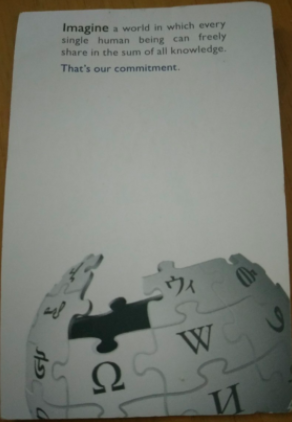
\includegraphics[width=.4\textwidth]{Images/cartao_wmf.png}
    \caption{Verso do cartão de visitas dos funcionários da Wikimedia Foundation.}
    \label{fig:cartao_wmf}
\end{figure}



\newpage

\subsection{Todos/as podem editar?}

Todos/as podem editar a Wikipédia, mas a tarefa não é tão fácil quanto pode parecer. É amplamente documentada a dificuldade de entrada de novos/as editores/as \citep{antin_my_2011}; \citep{burke_feed_2009}; \citep{faulkner_etiquette_2012}; \citep{halfaker_rise_2013}; \citep{kraut_dealing_2010}; \citep{morgan_tea_2013}; \citep{schneider_accept_2014}; \citep{steinmacher_social_2015}. Existem várias regras que dizem o que pode ou não ser escrito, e muitas delas já estão naturalizadas nas ações cotidianas dos/as usuários/as experientes e também nos softwares que gerenciam e atuam na enciclopédia.

Este trabalho pretende pesquisar a aplicação destas regras, entendendo seu histórico de criação, seu processo de naturalização e os efeitos que causam nos/as novatos/as que são pegos/as de surpresa ao tentar editar, e não tem ideia de todo o complexo mundo de governança da enciclopédia.

A Wikipédia é o décimo site mais acessado do mundo, e o décimo-quinto do Brasil. Em ambos os rankings é o site mais visitado mantido por uma instituição sem fins lucrativos \citep{alexa_2019}. No ano de 2019, apresentou uma média de 500 milhões de visitantes únicos por mês \citep{wikimedia_stats_2019}. Os imponentes números de sua audiência dizem que uma informação que perdure na Wikipédia tenderá a ser lida por milhares de pessoas e replicada indefinidamente, o que nos mostra a grande relevância desta ferramenta no mundo contemporâneo e sua centralidade na construção de fatos em nosso tempo.

Todos esses acessos estão distribuídos entre mais de 40 milhões de verbetes escritos em diferentes 303 idiomas, que atualmente são mantidos por aproximadamente 400 mil editores/as ativos/as \citep{wikimedia_stats_2019}. No momento, a versão lusófona conta com um pouco mais de um milhão de verbetes, mantidos por aproximadamente 3600 usuários/as ativos/as \citep{wikimedia_stats_2020}\footnote{Dados encontrados em https://stats.wikimedia.org/\#/pt.wikipedia.org/contributing/active-editors/normal|line|2-year|~total|monthly , acessada em 12/02/2020.}. É inquestionável que seus números de editores são grandiosos, e a um primeiro olhar esse volume pode parecer sustentar a afirmação de que afinal "\textit{qualquer um/a pode editar}".

A primeira cena apresentada versa sobre Jimmy Wales, um dos fundadores da Wikipédia e diretor executivo da Wikimedia Foundation até 2007. Ao contrário do que se poderia achar, sua saída da fundação, há mais de uma década, não fez desaparecer o discurso aqui posto à prova pelas cenas. Sua sucessora, Sue Gardner, manteve a linha do discurso, como pode ser visto em diversas falas\footnote{Publicação feita em seu blog pessoal acessada em 12/02/2020. https://suegardner.org/2013/01/14/the-people-behind-wikipedia-the-encyclopedia-anyone-can-edit/ .}, palestras\footnote{Palestra apresentada em 2010 e acessada em 12/02/2020 https://www.youtube.com/watch?v=vzJCHQ42XAw\&t=127s .} e entrevistas\footnote{Entrevista concedida em 2013 e acessada em 12/02/2020 https://www.youtube.com/watch?v=Y6gYhHWglBA .} concedidas ao longo dos 8 anos de sua gestão. Gestão marcada pela construção de programas que buscaram estimular a contribuição editorial de grupos sociais sub representados dentre os/as editores/as da enciclopédia, tais como moradores/as do sul global e mulheres, levantando uma bandeira que podemos tentar resumir em "todos/as devem ter condições de editar"\footnote{Esse discurso pode ser encontrado em diversos materiais, tais como esta entrevista dada em 2012 e acessada em 12/02/2020 https://www.youtube.com/watch?v=UoWgqPcF-TQ .}, mas sem jamais abandonar o "qualquer um/a pode editar".

A expressão "qualquer um/a pode editar a Wikipédia"\footnote{A expressão utilizada no buscador foi exatamente: "qualquer um pode editar" Wikipédia} é tão onipresente em discursos de \textit{hackers}, militantes da cultura livre, professores/as e até mesmo de seus/suas críticos/as que, uma rápida busca por ela no Google, retorna mais de 18 mil resultados. Indo além, ao testarmos a versão original da afirmação em inglês “\textit{anyone can edit Wikipedia}”\footnote{A expressão utilizada no buscador foi exatamente: "anyone can edit" Wikipedia}, a maior ferramenta de buscas do mercado retornou mais de 660 mil links\footnote{Buscas realizadas no endereço www.google.com em 28/01/2020.}.

Fazendo um recorte apenas por trabalhos acadêmicos, utilizando a ferramenta Google Scholar\footnote{Busca realizada no serviço https://scholar.google.com em 28/01/2020.}, nos foram apresentados mais de 3 mil trabalhos com o referido termo em inglês. Esse enorme volume sustenta que nossa cena inaugural não está descolada da realidade, e reforça a popularidade do termo, inclusive dentre os/as estudiosos/as da enciclopédia virtual.

É importante notar que o discurso está presente tanto na fala dos/as defensores/as do modelo distribuído da enciclopédia como na de seus/suas críticos/as. O que para alguns é visto como um diferencial competitivo, para outros é um problema irreparável. Não é difícil encontrar tanto falas de intelectuais como expressões da cultura popular do mundo digital contemporâneo, através dos memes\footnote{Diversos exemplos de memes podem ser encontrados em buscas como https://www.google.com/search?q=meme+wikipedia+anyone+can+edit\&tbm=isch. Nos exemplos aqui exibidos na figura \ref{fig:memes}, a primeira imagem está escrito sobre a vítima ``Usando Wikipédia como fonte'' e sobre o atirador ``Mas qualquer um pode editar''. Segunda imagem: acima da professora está escrito ``Você não pode utilizar a Wikipédia como fonte'', e abaixo "qualquer um pode editar".}, atacando a Wikipédia exatamente por qualquer um poder editá-la. A própria Wikipédia mantém um verbete chamado ``Críticas à Wikipédia'', e dos seus 39 tópicos, o primeiro a ser apresentado é não por acaso chamado ``Crítica ao conteúdo'', que apresenta um texto de Robert McHenry, editor da Encyclopædia Britannica, afirmando não ser possível existir a fiabilidade enciclopédica em uma obra editável abertamente. \citewiki{ptwiki_criticas}\footnote{Sempre que uma página de uma Wikipédia for citada durante o estudo ela será referenciada seguindo o padrão: (``idioma'', ``nome da página'', ``data da edição'').}

\begin{figure}[H]
    \centering
    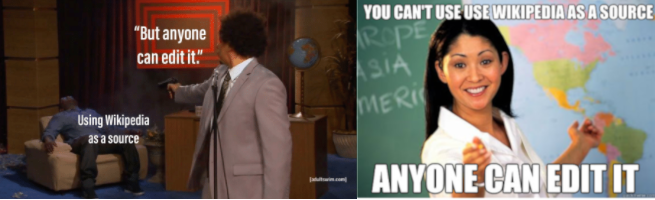
\includegraphics[width=1\textwidth]{Images/memes.png}
    \caption{Exemplos de memes sobre a Wikipédia.}
    \label{fig:memes}
\end{figure}

Os questionamentos de críticos relacionados a impossibilidade de se manter uma enciclopédia de qualidade que "qualquer um/a possa editar" são recorrentemente explorados e discutidos por professores/as, conteudistas, jornalistas e pesquisadores/as. Nestes questionamentos diversos fatores são colocados em xeque, mas invariavelmente todos assumem como verdade a afirmação de que "qualquer um/a pode editar". Não encontramos na literatura esforços para testar esta assertiva, esmiuçando o discurso propagado por todos os lados, sustentado em seus grandiosos números globais e na estrutura de uma ferramenta wiki aberta e colaborativa.

Assim, iremos nas próximas seções iniciar esforços de verificação na prática cotidiana, na vida real dos ``qualquer uns/umas'', a consistência deste discurso.

\newpage

\section{A nada mole vida dos wikipedistas}

\singlespacing
\begin{flushright}
\textit{``Eu só voltei}

\textit{Pra te contar}

\textit{Viajei}

\textit{Fui pra Serra do luar}

\textit{Eu mergulhei}

\textit{Ah, eu quis voar}

\textit{Agora vem}

\textit{Vem pra terra descansar''}

Walter Franco

\end{flushright}
\doublespacing

\subsection{Para onde vai um conteúdo reprovado?}

\textbf{Cena 3, Abril de 2017.\footnote{Cena escrita a partir de entrevista realizada com Alberto Lima no Rio de Janeiro, no dia 06 de fevereiro de 2020. Quando não explicitamente atribuídas a outrem, todas as aspas desta sessão são falas do entrevistado.} Rio de Janeiro.}

O engenheiro Alberto Lima, professor do curso técnico em Eletrônica do CEFET/RJ, liga seu computador decidido a criar o verbete ``Andes-SN'' na Wikipédia, para falar sobre o Sindicato Nacional dos Docentes das Instituições de Ensino Superior.

Concursado em 2011, Alberto participou ativamente do movimento grevista de 2012, greve esta deflagrada pelas bases em assembleia, contrariando indicação das direções sindicais. Após integrar o comando local de greve, inclusive participando de grandes atos em Brasília/DF, Alberto se junta a companheiros/as paredistas em 2013, concorre, e ganha a eleição para a direção da Adcefet-rj, seção sindical do Andes em sua instituição.

Ao final de sua gestão como presidente do sindicato local, em 2017, Alberto acreditava que o Andes-SN, apesar de ser um dos maiores sindicatos do Brasil, com seções em todas as universidades federais, não possuía uma grande presença digital. Resolveu ler sobre boas práticas de criação de verbetes na Wikipédia e, apesar da dica encontrada de começar editando artigos pré-existentes ao invés de criar um novo do zero, sentiu-se preparado para criar um verbete. Pesquisou se existiam artigos sobre outras entidades similares à sua, e se lembra de ter encontrado vários, ``\textit{alguns inclusive bem curtos com apenas uma referência}''. Com sua pesquisa feita, sentiu-se confiante e começou a escrever sobre seu sindicato nacional.

O professor nos conta que começou a escrever direto na página da Wikipédia. Fez um texto longo, ``\textit{que tinha inclusive uma ligação interna}'', duas referências e estruturado com ``\textit{Introdução} e "\textit{contextualização}''. Se sentia seguro e confortável ao escrever alí, pois afinal ``\textit{qualquer um pode editar a Wikipédia}''.
	
Sabia que seu texto ``\textit{não estava completamente redondo}'', mas resolveu salvar como estava para continuar mais tarde. Nosso editor novato nos conta que já tinha visto alguns verbetes na Wikipédia marcados com avisos como ``\textit{esboços}'', ``\textit{demandando estruturação}'' ou ``\textit{carece de referências}'', e sabia que a mesma coisa poderia acontecer com seu verbete, que seria melhorado mais tarde.

Porém, alguns segundos depois ele é surpreendido por uma notificação informando que seu artigo havia sido removido pelo administrador EVinente, atendendo a um pedido de outro usuário. Ao acessar o endereço da página, se deparou com a seguinte imagem:

\begin{figure}[H]
    \centering
    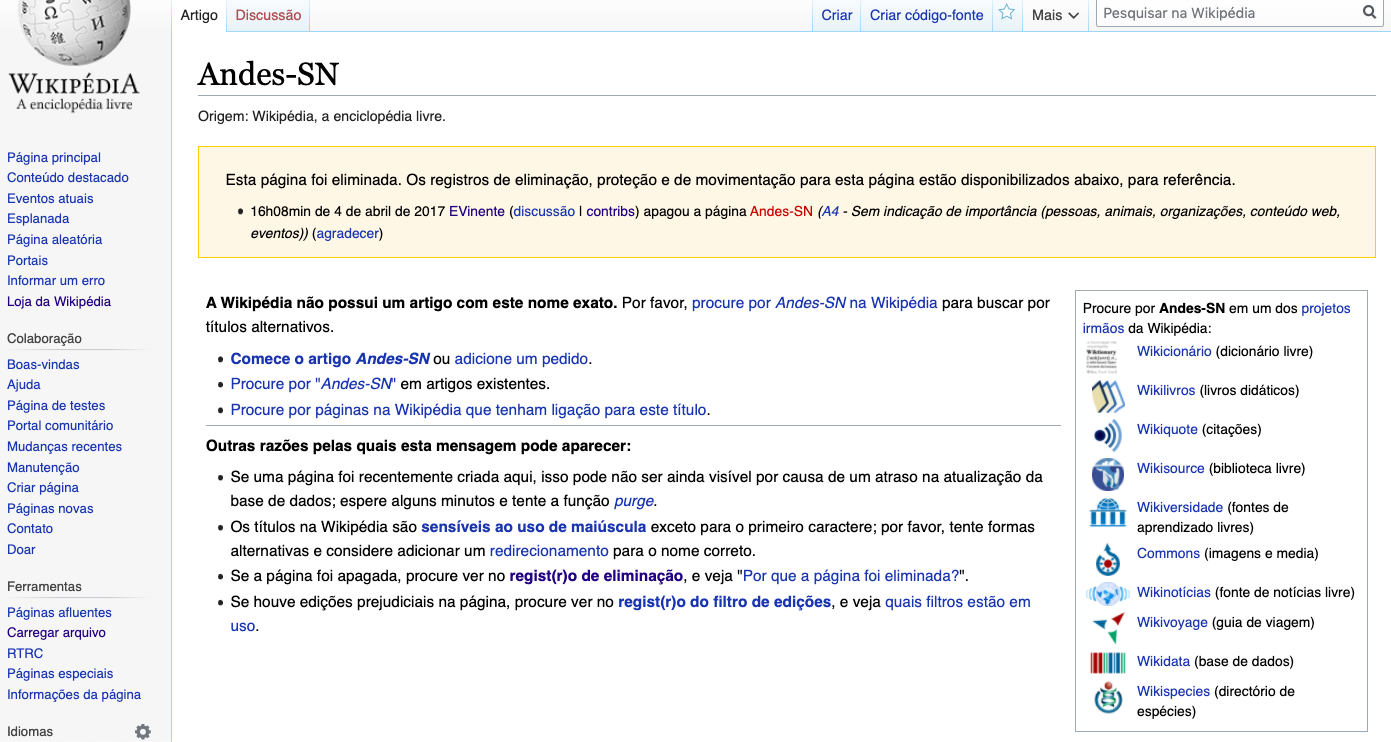
\includegraphics[width=1\textwidth]{Images/andes.png}
    \caption{Verbete Andes-SN com aviso de eliminação.}
    \label{fig:verbete_andes}
\end{figure}

Lembrando das apresentações assistidas nos seminários de pesquisa sobre controvérsias na Wikipédia, Alberto vai à página de discussão do usuário que solicitou a eliminação, onde o profesor então explica saber que o verbete ainda não estava ideal, que teria mais referências para adicionar (``\textit{notícia de greve é o que mais tem}''), inclusive com uma tese acadêmica sobre a história do sindicato. Concluiu informando que gostaria de continuar editando.

\begin{figure}[H]
    \centering
    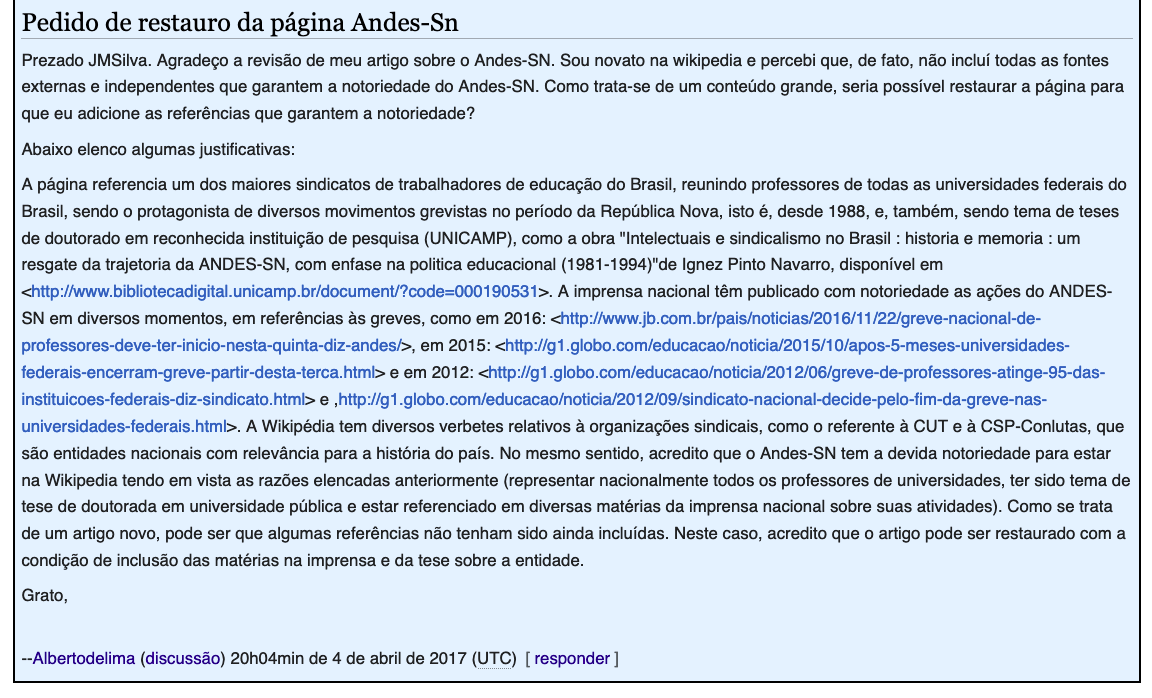
\includegraphics[width=1\textwidth]{Images/alberto-pedido-restauro.png}
    \caption{Página "Wikipédia:Pedidos/Restauro" com o pedido de Albertodelima para que a solicitação remoção feita por JMSilva fosse revista.}
    \label{fig:pedido_restauro_andes}
\end{figure}


O Diálogo então, segundo a memória de nosso protagonista, seguiu mais ou menos assim:

-Se você já sabia onde encontrar mais referências por que não as colocou logo?

-Eu estava sem tempo, mas vou colocar. Porém, o que eu já escrevi sumiu. Quero editar e melhorar, mas não tenho backup.

- Você vai ter que escrever tudo de novo.

Alberto, traído pela confiança na ferramenta, não seguiu sua prática corriqueira de escrever offline e depois "copiar e colar" o conteúdo criado em uma ferramenta online, e agora se via sem possibilidade de acessar novamente sua criação, eliminada do histórico público da Wikipédia.
Como resultado, ele, que estava ocupado com a reta final de seu mandato à frente da Adcefet-rj e já cursando doutorado, resolveu abrir mão de disputar a construção de conteúdos na Wikipédia. ``\textit{Eu nunca mais criei nenhum outro artigo. Nem esse.}''

No início de 2020, Alberto ficou feliz em ver que fora criado em 2018 outro verbete sobre o Andes-SN, desta vez levando seu nome completo, ``Sindicato Nacional dos Docentes das Instituições de Ensino Superior''. Apesar do novo verbete ser muito inspirado na seção ``Sobre'' da página sindicato, não apresentar nenhuma referência, ser muito menos acadêmico que o anterior, e de ter recebido as marcações de ``\textit{Este artigo não cita fontes confiáveis e independentes}'' e ``\textit{Este artigo é um esboço}'', em nenhum momento foi ``proposto para eliminação''.
\newpage
\subsection{Engajamentos e desengajamentos}

\textbf{Cena 4, Janeiro de 2016. Niterói, Brasil.\footnote{Cena escrita a partir de entrevista realizada com Carlos Eduardo Mattos da Cruz no Rio de Janeiro, no dia 06 de fevereiro de 2020. Quando não explicitamente atribuídas a outrem, todas as aspas desta sessão são falas do entrevistado.}}

Carlos Eduardo Mattos da Cruz, responsável pela criação de cursos para os telecentros do município\footnote{Espaços criados para o desenvolvimento de atividades educacionais complementares pelo Programa Niterói Digital, desenvolvido pela Secretaria Municipal de Educação, Ciência e Tecnologia de Niterói.}, orgulhosamente recebe o coordenador do Wiki Educação Brasil, grupo local reconhecido pela Wikimedia Foundation, para iniciar o curso de capacitação de professores/as da rede municipal no uso dos projetos Wikimedia, seguindo a proposta dos telecentros de oferecer uma ``\textit{educação contemporânea sem a ditadura do MEC}''.

O projeto desta formação foi desenvolvido por Cadunico, como Carlos gosta de se apresentar, a partir de conversas com funcionários da Wikimedia Foundation, que contaram-lhe sobre como os projetos educacionais com a enciclopédia só aconteciam em universidades, e que havia o desejo de diversificar o perfil dos editores e levar a prática de escrita wiki para outros níveis educacionais.

Cadunico decidiu tocar o projeto mesmo tendo experiências pessoais não agradáveis no mundo das wikis. Em julho de 2012, criara um verbete sobre o Gnugraf, maior evento de softwares livres para edição gráfica da América Latina, organizado por ele e por sua esposa Cléo Mattos. Pouco tempo depois, foi surpreendido com a remoção do verbete. Através do apoio de amigos que trabalhavam para o movimento e de um editor experiente, conseguiu, ``\textit{depois de muito sufoco}'', deixar no ar uma versão bem simplória do texto original. Até hoje Cadunico tem receio de editar o verbete e adicionar mais informações, para não ``\textit{chamar a atenção}'' de revisores, que podem novamente decidir apagá-lo, assim como aconteceu com sua página de usuário.

Foi em maio de 2013 que ele teve sua página de usuário apagada na Wikipédia. Em suas palavras, ``\textit{porque coloquei mais um item em uma lista de coisas que eu já tinha feito e um robô bloqueou a página}''. Curiosamente, ao observarmos o histórico da página, vemos que a ação não havia sido realizada por um robô, e sim por um dos usuários humanos mais ativos da Wikipédia lusófona. Perguntado sobre mensagens recebidas em sua página de discussão, Cadunico disse desconhecer tal ferramenta, e emendou: ``\textit{quando entro no Facebook pela primeira vez ele tem umas setinhas e umas formas de mostrar onde estão as coisas. Não me lembro de ter visto isso quando me cadastrei na Wikipédia. Só utilizei a 'caixa de areia'\footnote{Área da Wikipédia onde editores podem realizar testes.} por que eu já tinha conversado com pessoal da fundação que me falou dela. Mas ainda assim, a gente escreve lá e ninguém lê. Ninguém te dá dicas sobre o que melhorar antes de enviar conteúdo para o artigo}''.

Após frustrar-se com a Wikipédia, Cadunico ``se muda'' para o Wikilivros, projeto do Movimento Wikimedia para escrita de livros didáticos. Consegue com sucesso criar uma apostila para utilização do software de diagramação \textit{Scribus}\footnote{Apostila disponível em  https://pt.wikibooks.org/wiki/Apostila\_de\_Scribus , acessada em 30 de março de 2020.}, retomando assim sua confiança na possibilidade de trabalhar em conjunto com o movimento.

Então, em 2015, Caudnico convidou representantes do Movimento Wikimedia, que trabalhavam em conjunto com a Fundação, para serem responsáveis pela formação dos/as professores/as. Acreditou que essa chancela evitaria que situações desagradáveis como as vividas por ele na Wikipédia se repetissem. ``\textit{Eu queria botar nos telecentros o símbolo da Wikimedia, e falar que aqui é um núcleo oficial, com aula dada pelo pessoal da própria Fundação. Fizemos banners e tudo mais}''.

A meta do projeto era fazer com que professores da rede municipal de Niterói adotassem ferramentas wiki em suas práticas pedagógicas. A ideia era o/a professor/a editar em suas horas fora de sala de aula, bem como editar com seus/suas alunos/as. Para além da Wikipédia, eles/elas seriam estimulados a escrever livros didáticos em conjunto no Wikilivros e inclusive a compartilhar seus planos de aula no Wikiversidade. O projeto ainda previa, em um segundo momento, expandir a capacitação para a Secretaria de Turismo, que poderia ajudar a manter verbetes na Wikipédia sobre a cidade de Niterói.

O projeto era grandioso. Contaria com ciclos de dois anos, com um ano de capacitação seguido de um ano com os/as professores/as atuando de forma independente, e no ano seguinte um novo ciclo se iniciaria, com nova formação para reciclagem e aprofundamento. Os encontros aconteciam no Telecentro do Terminal Rodoviário João Goulart. ``\textit{Era o maior telecentro, com a melhor internet e as melhores máquinas}''. Por duas vezes na semana, a equipe de lá parava de atender os outros telecentros (o escritório de gestão de todos os telecentros do município ficava nesta unidade e sua equipe auxiliava no suporte aos telecentros menores) para se dedicar exclusivamente à capacitação Wikimedia.

``\textit{Treinamentos como este começam cheios e terminam vazios. Mas com este foi diferente. Começou cheio e terminou mais cheio ainda.}'' O boca a boca entre os/as professores/as era intenso. Todo dia um/a professor/a ligava perguntando se ainda tinha vaga, e a política da Secretaria de Educação era sempre falar que tinha, para depois se virar em acomodar todo mundo. Um dia Cadunico foi convocado pelo secretário de educação, que queria monitorar o maior problema das capacitações ofertadas no município:

- E aí, como está a evasão?

- Não teve evasão.

- Que bom, então todos os alunos que começaram terminaram?

- Mais ou menos.

- Não estou entendendo.

- Começamos com um aluno por micro, e terminamos com três.

Após um ano de treinamento, era chegado o momento dos/as professores/as criarem conteúdos sem apoio de instrutores experientes. Se aproveitando de práticas de acompanhamento da aplicação dos conteúdos dos cursos com feedback contínuo dos professores, desenvolvidas no projeto "Academia de Jogos", que ensinava a criação de softwares educacionais para crianças e professores, a Secretaria de Educação seguiria então ao longo do ano monitorando de perto a fase do projeto de edição nas wikis.

``\textit{Aconteceu com eles o que aconteceu comigo}'', conta Cadunico. ``\textit{Não era a grande maioria. \textbf{Todos estavam frustrados}. Os professores não conseguiam ter o gosto de ver seus conteúdos publicados}''. Cadunico acrescenta que um professor de história da escola municipal do Fonseca, autor de uma tese acadêmica sobre Niterói antiga, e o mais empolgado durante a capacitação, ``\textit{foi sumariamente censurado e desistiu}''.

E não foram só os professores. Novamente Cadunico se sentiu censurado pelo movimento que ele tanto admirava por ter ``\textit{a missão mais nobre do planeta: a de disponibilizar livre e gratuitamente todo o conhecimento humano}''. Enquanto os professores trabalhavam com as wikis, Cadunico resolveu começar um livro didático no Wikilivros. Um livro de pensamentos que, assim como sua página na Wikipédia, foi apagado. A justificava dada para o apagamento sentensiava que seu material não era considerado um livro didático, sem que Cadunico tivesse recebido qualquer aviso, tentativa de diálogo ou chance de defesa. ``\textit{Um livro de pensamentos não é um livro didático para ensino de português ou literatura? Isso é uma forma de censura. Não deixam explícito que tipo de livro é aceitável ou não, o que já acho errado pois para mim todo livro é aceitável, e simplesmente arrancam seu trabalho, de forma impessoal e muito fria.}''

Independente das frustrações, o projeto seguia o cronograma planejado. Depois de passado meio ano de atividades de escrita wiki sem acompanhamento dos especialistas wikipedistas, a secretaria avisou aos/às professores/as que no início do ano seguinte começaria uma nova turma do projeto, buscando levantar a demanda para realizar seu planejamento. Vários/as professores/as pediram para não acontecer uma próxima versão, solicitando que a secretaria criasse outro projeto, pois eles/as estariam sendo censurados/as e maltratados/as na Wikipédia. ``\textit{Tínhamos conseguido um pequeno exército para editar conteúdos brasileiros, e ele foi se desmotivando e se dissolvendo}''. Perante tantos retornos negativos e nenhum caso de sucesso, o projeto foi cancelado e o segundo ciclo nunca se inicio.

Em paralelo, os telecentros promovíam capacitações de LibreOffice, em parceria com Eliane Domingos e Oliver Hallot, da Associação Libre de Técnicas Abertas (ALTA), parceira local da The Document Foundation\footnote{Organização mantenedora do software LibreOffice.}. Estas capacitações, que formaram mais de 30 mil pessoas, tiveram como contrapartida da equipe de Niterói o compromisso de manter a wiki com a documentação do LibreOffice em português atualizada. ``\textit{O que foi fácil, pois os professores já haviam aprendido a utilizar o MediaWiki nos cursos da Wikimedia}''.

Os/as professores/as de inglês acompanhavam a lista de e-mails dos/as desenvolvedores/as do LibreOffice e passavam para colegas as necessidades de atualização da wiki. A versão em português da documentação era atualizada em tempo real, muitas vezes mais rápido que em inglês. Neste projeto a equipe ficou muito motivada, com professores/as editando inclusive em suas horas vagas, relatando se sentirem úteis e valorizados/as. ``\textit{No LibreOffice ninguém os revertia. Provando que o problema nos projetos Wikimedia não eram ocasionados por falta de qualidade de nossa equipe.}'' \citep{cadunico_2020}
\newpage
\subsection{Comunidade local decisões globais }

\textbf{Cena 5. Junho de 2017. Rio de Janeiro, RJ.}

A disciplina ``Estudos CTS (Ciências-Tecnologias-Sociedades): aproximações brasileiras e latino-americanas'' é ministrada no Programa de Engenharia de Sistemas e Computação da COPPE/UFRJ no 2º período de 2017. A turma é convidada a ler o capítulo 7 do livro ``\textit{Yes, nós temos Pasteur. Manguinhos, Oswaldo Cruz e a história da ciência no Brasil}'' \citep{cukierman_pasteur_2007}, intitulado ``\textit{Prata Preta}''.

``\textit{Chamava-se Horácio José da Silva, mas, que importava?}'' \citep[p. 220]{cukierman_pasteur_2007}. A frase que abre o capítulo citado se refere ao Prata Preta, um personagem da Revolta da Vacina ocorrida no Rio de Janeiro, em 1904, que, como tantos outros tipos, não é encontrado nas narrativas universalizantes da história da ciência brasileira. A leitura, que narra momentos decisivos para a construção sociotécnica das ciências brasileiras pelo ângulo de um personagem que não pensaríamos \textit{a priori} como protagonista, provoca algumas reflexões: a quantos outros/as anônimos/as da história da ciência e tecnologia brasileiras a frase de abertura poderia se referir? Como se faz educação em ciências contextualizada em um país com tantos/as atores/atrizes sem voz? Em espaços populares, fora das salas de aulas dos programas de pós-graduação, quais histórias são contadas e quais versões são aprendidas?

Após a leitura, com todas essas perguntas na cabeça, recebo uma provocação de meu colega de pós-graduação, o doutorando Fernando Severo: ``\textit{vamos melhorar o verbete sobre o Prata Preta na Wikipédia?}''. Imediatamente aceito o convite e vamos analisar o material já existente na enciclopédia. Percebemos então que o verbete biográfico de Prata Preta possuía apenas 1754 bytes\footnote{Unidade de medida utilizada pela comunidade Wikimedia para medir o tamanho de revisões e verbetes.}, sendo a metade deles sobre um bloco de carnaval que leva seu nome.

\begin{figure}[H]
    \centering
    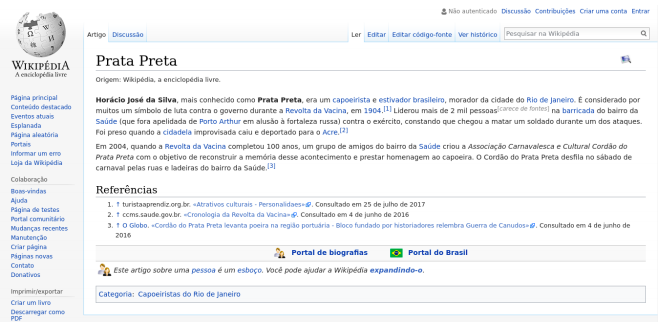
\includegraphics[width=1\textwidth]{Images/pratapreta.png}
    \caption{Versão do verbete Prata Preta encontrado no dia da cena.}
    \label{fig:verbete_pratapreta}
\end{figure}

Aceito o desafio de melhorar o verbete e, enquanto penso sobre os desafios de escrever uma biografia de um subalterno sem voz, com poucas fontes secundárias fiáveis versando sobre sua história, faço uma singela edição com pequenos ajustes ao texto que já estava lá. Para minha grande surpresa, a edição não é salva pela Wikipédia, que me informa: ``\textit{Seu IP está bloqueado}''.

Rapidamente descubro que na verdade não só eu, como milhares de usuários/as da Virtua, maior provedora de internet do Rio de Janeiro, já estavam bloqueados/as por três meses, como resposta a um suposto vandalismo excessivo feito em vários idiomas pelo mesmo range de IP. Essa drástica medida é tomada quando se entende que uma ação orquestrada de vandalismo estará se aproveitando de um provedor de acesso, VPN\footnote{Do inglês Virtual Private Network. São conexões entre máquinas na internet que direcionando o tráfego de uma sempre para a outra.} ou Proxy para mudar de IP constantemente e furar o bloqueio individual a um determinado IP individualizado. E pior, diferente da estratégia de bloqueio simples de IP, onde basta o/a editor/a criar uma conta de usuário/a para (agora rastreado) poder voltar a editar, o bloqueio de faixa de IP incluía também usuários/as registrados/as. Com isso, mesmo meu usuário, com milhares de edições e ficha corrida limpa na enciclopédia, estava proibido de editar.

Fomos então estudar o histórico de edições feitas em nossa faixa de IP e nos surpreendemos com o resultado! Como pode um usuário holandês, que aplicou o bloqueio em todos os sites do Movimento Wikimedia, ter colocado no mesmo balaio de gato Fernando Severo, eu, o IP 179.210.26.120, que estava escrevendo sobre uma escola de samba teresopolitana em português, e o IP 179.210.99.239, que editava sobre a série televisiva ``Meu Pequeno Pônei'' em galego? Não terá seu olhar saxão sido capaz de perceber a distância entre interesses tão distintos e ações de edição? Terá ele conseguido ver apenas uma horda anárquica subdesenvolvida que não tem modos nem educação para escrever uma enciclopédia!?

Saímos então da periferia que é a Wikipédia lusófona e fomos buscar os centros globais de tomada de decisão da enciclopédia. Estudamos as políticas de acesso e de bloqueio globais da comunidade Wikimedia e fomos parar em uma sala de chat em inglês no IRC.\footnote{Do inglês \textit{Internet Relay Chat}, ferramenta para criação de salas de bate papo virtuais.} Lá conversamos com os/as ``gringos/as'', relatando detalhadamente ``o causo'', procurando esclarecê-los a respeito da estrutura do mercado de internet no Rio de Janeiro, com milhões de usuários/as e poucos provedores de acesso; das diversas edições feitas em diferentes wikipédias por editores em nosso range de IP; da forma dinâmica como funciona a distribuição de IP nos provedores de internet; do longo histórico de bom comportamento de meu usuário. Vários/as aliados/as foram convocados/as ao esforço de demonstrar que nosso grupo nada homogêneo, unido involuntariamente por uma faixa de endereços de IP, tem seu valor para a comunidade, e pode ser produtor de conhecimento. Recebi uma desanimadora resposta burocrática de um anglófono, que simplesmente mandou enviar e-mail para um determinado endereço e esperar por um resposta sem prazo.

Mas, eis que de onde parecia que não surgiria mais alento, emerge a empatia de um \textit{steward}\footnote{No Movimento Wikimedia são usuários com permissões para administrar todas as wikis de todos os projetos.} falando português. Ele se solidariza com nosso pleito e nos autoriza a participar novamente do jogo global de construção de conhecimentos na wiki universal, relaxando parcialmente o bloqueio. Agora, após nossa expedição exploratória da implementação da política de bloqueios globais do Movimento durar toda a madrugada, poderíamos novamente editar, desde que estivéssemos devidamente registrados no site com um usuário próprio. Usuários/as anônimos/as continuariam impedidos/as de editar. Afinal, nosso pleito ``tinha seu valor sim, mas também não era para tanto, né?''. Com a confirmação de que havíamos conseguido superar a pane, compondo um novo arranjo suficiente para estabilizar o funcionamento da Wikipédia para nossos usuários, fomos dormir às 5 horas da manhã, sem realizar nenhuma edição no verbete de Prata Preta.
\newpage
\section{Cenas corriqueiras inspiram projeto de pesquisa}

As cenas que acabaram de ser apresentadas ilustram um distanciamento entre o onipresente discurso de que a Wikipédia é a ``enciclopédia que qualquer um/a pode editar'' e a prática que emerge quando os ``qualquer uns/umas'' de fato se aventuram a criar conteúdos lá. Invariavelmente eles/as acabam se deparando com barreiras não óbvias, tais como regras editoriais complexas, robôs reversores, revisores apressados, filtros de edição ou administradores/as impacientes.

Cotidianamente a Wikipédia convive com esta dicotomia entre ser aclamada como o maior projeto de produção compartilhada de conhecimento da história da humanidade, onde ``todos podem editar'' e ser acusada de não estar aberta para receber colaborações que não estejam perfeitamente enquadradas em um determinado padrão.

São incontáveis os casos de pessoas que, mesmo familiarizadas com movimentos de cultura livre e com dinâmicas educacionais, como os/as personagens de nossas cenas, ao se aventurarem no mundo onde ``qualquer um pode editar'' encontram barreiras relacionadas a ``o que pode ser editado''. Ao mesmo tempo, wikipedistas que propagam o discurso de que ``qualquer pode editar'', e se orgulham desta abertura de seu projeto, parecem não enxergar estas barreiras, que para editores/as experientes teriam soluções óbvias.

Assim sustentamos a motivação desta pesquisa em estudar as controvérsias em torno do discurso exultante de que ``\textit{qualquer um/a pode editar a Wikipédia}''. Inspirados por cenas que insinuam a não obviedade do discurso buscamos neste trabalho abrir caixas-pretas, entendendo as dificuldades e barreiras encontradas por novos/as editores/as que buscam editar a Wikipédia em português, e como regras se naturalizam no cotidiano da operação da enciclopédia, tanto em forma de comportamentos como de softwares.

Nossa pesquisa é focada na versão em português da Wikipédia. Esta informação, que pode parecer trivial para alguns/algumas, é relevante de ser explicitada pois apesar de muito estudada, a Wikipédia vê a maioria dos/as pesquisadores/as que se aproximam dela interessados em sua original e maior versão; a desenvolvida em língua inglesa. 

É muito difícil, para não dizer impossível, saber quantas pesquisas já foram desenvolvidas sobre a Wikipédia. Um esforço feito no início da década pelo projeto Wikipapers, e desatualizado desde 2013, tentou desbravar tal empreendimento. Em sua última atualização, o projeto havia mapeado 2588 trabalhos. Destes, apenas 1,7\% do total eram escritos em língua portuguesa (\cite[68]{esteves_as_2014}). Desde então o número de pesquisa em português sobre a Wikipédia pode ter subido um pouco, motivado pela realização de duas edições do Congresso Científico Brasileiro da Wikipédia (CCBWIKI) e mais duas do International Wiki Scientific Conference (IWSC), que apesar de trilíngue (inglês, espanhol e português), teve suas duas edições inaugurais realizadas em cidades lusófonas (Niterói no Brasil e Porto em Portugal), atraindo em sua maioria trabalhos escritos em português e totalizando mais de 30 trabalhos apresentados em português em todas suas edições.

Ainda assim, este volume de pesquisas lusófonas é muito pequeno perante a produção global. Uma busca rápida no Google Scholar pelo termo "Wikipedia" retorna ``\textit{aproximadamente 1.500.000 resultados}''\footnote{https://scholar.google.com.br/scholar?as\_vis=1\&q=Wikipedia\&hl=pt-BR\&as\_sdt=1,5, acessada em 06/03/2020.}, enquanto uma busca na mesma ferramenta, com o filtro ativado para trabalhos em português, retorna ``\textit{aproximadamente 59.700 resultados}''\footnote{https://scholar.google.com.br/scholar?lr=lang\_pt\&q=Wikipedia\&hl=pt-BR\&as\_sdt=1,5\&as\_vis=1, acessada em 06/03/2020.}. Se, por um lado, o Brasil é responsável pela produção de aproximadamente 2,5\% dos \textit{papers} do mundo\footnote{Número retirado de uma palestra apresentada pelo Ministro de Estado de Ciência e Tecnologia em 2011 (MERCADANTE, 2011 apud \cite{cukierman_uma_2011}) que, mesmo desatualizado, acredito ser um retrato próximo ao cenário que temos hoje.}, por outro, a participação de trabalhos lusófonos no corte buscado no Google Scholar fica em 0,04\%. Sabemos que esta busca simplória não retorna apenas trabalhos sobre a Wikipédia, e muitas publicações com outros objetos de estudo podem citar brevemente o nome "Wikipedia" e acabarem sendo somadas neste montante, mas este fenômeno de menção marginal ao termo pode acontecer em qualquer idioma, podendo ser descartado como uma das causas da disparidade. Assim, não é exagero supor que a mesma distância no volume de trabalhos produzidos entre idiomas citando o termo "Wikipedia" continuará existindo para trabalhos especificamente sobre a Wikipédia. 

Ademais, cabe também observarmos que nosso recorte linguístico tem ainda um fator transbordado que se levado em conta ampliará a distância entre conteúdos produzidos sobre cada versão da enciclopédia. Dentre os estudos realizados sobre a Wikipédia, dada a dinâmica de centros e periferias globais da ciência, é comum encontrar publicações feitas em diversos idiomas, português incluso, estudando a Wikipédia em inglês. Já a recíproca não é verdadeira. É de se esperar que a vasta maioria dos trabalhos em outros idiomas não olhem para uma versão menor e escrita em um idioma não falado nos grandes centros de pesquisa como a Wikipédia lusófona, aumentando ainda mais a distância de pesquisas produzidas entre as diferentes Wikipédias.

Por fim, apesar de una para toda a lusofonia global, cabe destacar a relevância da Wikipédia em português para o Brasil. Na Wikipédia não existem versões para as diferentes variações da língua portuguesa faladas pelo mundo e, brasileiros, portugueses e demais lusófonos convivem no mesmo projeto. Em meio toda comunidade global, a versão em língua portuguesa da enciclopédia é majoritariamente frequentada por brasileiros, que em fevereiro de 2020 foram responsáveis por 56\% dos acessos. Curiosamente, em segundo lugar no ranking de visitas ao site aparecem os Estados Unidos com 9,8\% dos acessos, a frente de Portugal com 8,4\%. Cabe destacar também que após os três primeiros colocados nenhum outro país apresenta um volume relevante de acessos, com nenhum dos demais apresentando mais de 1\% dos acessos.\footnote{Dados obtidos na ferramenta Wikimedia statistics, https://stats.wikimedia.org/\#/pt.wikipedia.org/reading/page-views-by-country/normal|table|last-month|~total|monthly} Esse volume de acessos tupiniquim, que representa em valores brutos 220 milhões de \textit{pageviews} ao mês, não deixa dúvida sobre a importância da Wikipédia em português para os/as brasileiros/as, e sustenta a relevância de sua escolha como objeto de pesquisa.

Esta realidade então nos motivou a enfocar esse estudo, feito no Brasil e em português, na Wikipédia lusófona.

\subsection{O autor desta dissertação pode editar?}

\singlespacing
\begin{flushright}

\textit{``Tudo é uma questão de manter}

\textit{A mente quieta}

\textit{A espinha ereta}

\textit{E o coração tranquilo''}

Walter Franco

\end{flushright}
\doublespacing

Para proporcionar ao leitor uma apreciação situada deste trabalho, entendo ser importante explicitar aqui minha trajetória com a Wikipédia e sua comunidade. Sou militante do movimento software livre desde 2003, participando de diversas comunidades reunidas em torno de causas ligadas ao que chamamos de cultura livre, tanto a do desenvolvimento de software como a da evangelização de novos/as entrantes. Dentro destes movimentos, sempre foi corriqueira a prática de utilizar ferramentas wiki para documentar nossas atividades e construir \textit{sites} de forma colaborativa.\footnote{O TWiki, sistema mais popular de gestão de wikis do início do século teve sua primeira versão lançada em 1998 REFERÊNCIA: https://twiki.org/ .}

Em meados da década 2000 conheci a Wikipédia e, já habituado a ferramentas wiki, passei instintivamente a realizar edições pontuais como usuário anônimo. Em toda minha experiência com wikis, apenas tive usuário registrado naquelas em que a edição era restrita a cadastrados, pois não via sentido em criar uma conta em uma wiki que qualquer um poderia editar.

No dia 27 de Fevereiro de 2009 passei por uma surpresa. Ao acessar o site da Wikipédia vi em destaque no topo da página "\textit{Você tem uma mensagem nova}", e tive certeza de que se tratava de um bug da plataforma. Afinal, eu não estava logado, então não seria possível me enviarem mensagens. Decidido a investigar o bug cliquei no link, e, para meu espanto, a mensagem realmente era sobre uma edição feita por mim! Neste momento aprendi duas coisas: que a Wikipédia trata seus usuários anônimos pelo IP de conexão\footnote{Essa caraterística do MediaWiki será densamente explorada mais a frente na pesquisa.}, permitindo, ainda que de forma precária, rastreá-los minimamente; e que é importante ter um usuário cadastrado mesmo em uma wiki em que qualquer um pode editar, pois isso facilita a troca de mensagens com outros/as usuários/as editando o mesmo artigo que eu porventura também esteja editando.

Confesso um pouco de desconforto inicial com essa funcionalidade de mensagens associadas a usuários do MediaWiki. Outras ferramentas gestoras de wikis mais populares da época, como o TWiki e o TikiWiki, forneciam “apenas” páginas de discussão associadas a cada artigo criado, e não aos usuários. Assim, os debates giravam sempre em torno de uma página específica, e não existia a possibilidade enviar uma "mensagem direta" para um usuário. De cara imaginei que essa funcionalidade de mensagem direcionada a um usuário poderia deslocar discussões das páginas onde elas deveriam acontecer com mais visibilidade\footnote{Essa preocupação reaparecerá e será detalhada no capítulo 3.} além de também personificar as contribuições de uma maneira que me parecia não harmônica com a filosofia dos movimentos livres. Mas, como estava pessoalmente disposto a engajar-me com mais comunidades de produção de conteúdos, para além das comunidades de software, e percebendo a crescente importância da Wikipédia, dei o braço a torcer e criei meu usuário.

Desde então, meu usuário HenriqueCrang realizou 3368 edições nas wikis do Movimento Wikimedia, sendo 80\% delas na Wikipédia em português. Destas, 83,2\%, ou 2.182 edições\footnote{Dados de 03 de março de 2020, acessados em https://xtools.wmflabs.org/ec/pt.wikipedia.org/HenriqueCrang .}, foram feitas no chamado “domínio principal” da Wikipédia, que engloba as páginas com os verbetes enciclopédicos\footnote{A separação das Wikipédias em domínios será explicada no próximo capítulo.}.

Através de meu engajamento com redes de cultura livre, e curiosamente não pelas páginas da Wikipédia\footnote{Em alguns momentos da história os/as voluntários/a engajados em \textit{outreach} no Movimento Wikimedia no Brasil não estiveram próximos das atividades na Wikipédia em português. \textit{``Outreach''} é uma palavra em inglês que significa atividades extramuros, de extensão. Utilizaremos o termo em inglês pois a comunidade lusófona de wikipedistas utiliza-o corriqueiramente. Estas dinâmicas e separações serão melhor trabalhadas no capítulo 3.}, tive contato com o Movimento Wikimedia Brasil, que realizava atividades de \textit{outreach} para promoção das wikis, e passei a participar e organizar atividades no Rio de Janeiro. Em 2012, fiquei sabendo que a Wikimedia Foundation planejava abrir um escritório no Brasil\footnote{https://www1.folha.uol.com.br/fsp/tec/34745-wikipedia-abrira-seu-1-escritorio-no-brasil.shtml} e, ao final deste ano, candidatei-me e fui aprovado para trabalhar diretamente para a Fundação como “analista de dados e experimentos”. A ideia de abrir um escritório no Brasil acabou não vingando, mas tivemos uma equipe de quatro pessoas trabalhando no chamado “Programa catalisador do Brasil”, que buscava aumentar o número de editores ativos nos projetos Wikimedia no país, com especial foco na Wikipédia em português\footnote{Paralelamente foram realizados projetos similares na Índia e no MENA (sigla em inglês para Oriente Médio e Norte da África), regiões que foram mapeadas pela Fundação como apresentando uma baixa relação de editores/as\textbf{/}leitores/as, apresentando assim potencial para um rápido engajamento de novos/as voluntários/as.}.

Vale citar aqui que a Wikimedia Foundation tem como hábito criar um/a usuário/a “de trabalho” para seus funcionários, diferente de seu/sua usuário/a como voluntário/a. Como forma de separar o que era atuação da Fundação (que não financia diretamente a produção de conteúdo) e atuação voluntária, os/as funcionários/as que quisessem contribuir com as páginas de conteúdo deveriam fazê-lo com suas contas de voluntário/a, enquanto deveriam utilizar a conta institucional (normalmente com o nome terminado em “(WMF)” facilitando a identificação pela comunidade) para debater atividades nas quais estivesse atuando remuneradamente pela Fundação. Com meu usuário “HAndrade (WMF)” realizei mais 1612 edições, sendo a maioria delas no Meta Wiki e 36\% na Wikipédia em português.\footnote{Dados disponiveis em https://xtools.wmflabs.org/ec/pt.wikipedia.org/HAndrade\%20(WMF) , acessados em 03 de março de 2020.} Destas edições, 11 foram feitas por distração em verbetes, acreditando estar logado com a conta de voluntário.\footnote{É comum funcionários/as da WMF trabalharem com dois navegadores abertos, mantendo em um logada sua conta institucional e no outro sua conta de voluntário.}

Nestes anos em que trabalhei para a Fundação, atuei tanto auxiliando as comunidades lusófonas a desenvolver análises de dados para se conhecerem e testarem hipóteses, como também engajando voluntários/as técnicos/as para o desenvolvimento de ferramentas demandadas pelas comunidades locais. Estive assim imerso nas controvérsias da Wikipédia em português com disponibilidade, intensidade e dedicação muito maiores do que nos tempos de voluntário. Essa vivência me permitiu conhecer densamente o movimento e seus softwares, estruturas de dados, espaços de decisão e dinâmicas de governança. Tal experiência prévia serviu-me como um enorme e valioso mapa para navegar pelos espaços necessários para realizar essa pesquisa, que com certeza não teria sido desenvolvida da mesma maneira por um/a pesquisador/a recém chegado/a ao mundo Wikimedia.
\subsection{Para quem escrevemos?}

O presente estudo busca alcançar dois públicos-alvos de leitores/as. Pretende-se tanto atrair a comunidade de usuários/as engajados/as na governança da Wikipédia, como pessoas comprometidas com a realização de atividades para a atração de novos/as editores/as.

Ao mapear processos de tomada de decisão e expor as decisões automatizadas, tomadas por sistemas como o software MediaWiki e por robôs patrulhadores, este texto oferece para leitores/as wikipedistas experientes a oportunidade de refletir sobre a constatação de que a Wikipédia tem regras duras, muitas vezes nem conhecidas de sua própria comunidade, e que tendem a se naturalizar através de implementações em software e comportamentos precondicionados.

Olhamos para o histórico de tomadas de decisão da comunidade considerando a “\textit{indeterminação do passado, que (...) é a ideia de que o passado depende do presente e de como se reinterpreta hoje o que aconteceu ontem, sendo estas revisões verdadeiros esquemas de (re)organização do mundo}" (\cite[p.23]{feitosa_cidadao_2010}). Assim, sabendo que “\textit{estamos constantemente revisando nosso conhecimento sobre o passado à luz de novos desenvolvimentos do presente}” (\cite[40]{bowker_sorting_2007}), não tomaremos o dito senso comum da comunidade como verdade definitiva e recriaremos histórias com os enredamentos que cruzarem o caminhar da pesquisa.

Com esse movimento, espera-se oferecer aos/às membros/as da comunidade uma leitura que contribua tanto em momentos de criação de novas regras, como em discussões sobre aplicações de normas vigentes e em casos de enquadramentos/transbordamentos de exceções.

Concomitantemente, ao descrever detalhadamente a realização de editatonas, iremos agrupar práticas de organização desses eventos sugeridas pela comunidade global, expor números de resultados e descrever situações de conflito e resoluções, também fazendo desta obra uma possível referência para extensionistas do Movimento Wikimedia, envolvidos/as na organização de atividades de engajamento de editores/as novatos/as.

Também podem ser citados/as como potenciais leitores/as interessados/as nesta dissertação pesquisadores/as da área dos Estudos de Ciências-Tecnologias-Sociedades (CTS)\footnote{Optamos por esta forma de grafia para nos referenciar ao nosso campo de pesquisa, que pode ser encontrado em diferentes variações em outras obras. Latour, ao falar sobre os "\textit{Science Studies}", diz que "Nunca encontrei duas pessoas que estivessem de acordo quando ao significado do campo de estudo chamado "ciência, tecnologia e sociedade"; na verdade, raramente vi alguém que concordasse quanto ao nome ou quanto à própria existência do campo!" (\cite[p.25]{latour_ciencia_1987})}, que nas seguintes páginas encontrarão um estudo de caso que, não só lança mão de metodologias CTS, como também encontra e descreve práticas de produção de conteúdo com algumas similaridades à prática de produção científica, tão estudada por esta area. Ademais, ciente das diversas experiências desagradáveis sofridas por professores/as e pesquisadores/as ao tentarem editar a Wikipédia (são incontáveis os relatos de situações análogas às das cenas que abrem este trabalho), espera-se que este estudo possa demonstrar para leitores/as não-wikipedistas que a Wikipédia não é "gratuitamente cruel" com novatos/as, e que estes/as possam compreender as barreiras encontradas em suas tentativas de edição, e aprendam possibilidades de buscar desvios e composições em suas futuras disputas pela construção de conhecimento em wikis.
\subsection{Aliados da pesquisa}

O presente estudo somente se tornou possível pelo enredamento de diversos/as aliados/as que se interessaram e tiveram agência direta em atividades imprescindíveis para o trabalho. A começar por membros/as da Wikipédia, fossem administradores/as, editores/as ou desenvolvedores/as de ferramentas, que foram entrevistados/as e compartilharam seus conhecimentos e percepções sobre o funcionamento das comunidades wikipédicas.

Posteriormente, pude contar também com a ajuda de meus/minhas colegas da linha de pesquisa em Informática e Sociedade do Programa de Pós Graduação em Engenharia de Sistemas e Computação (PESC) da COPPE-UFRJ, que mobilizaram redes engajadas em seus trabalhos de campo para realizarmos editatonas. E, por fim, com as pessoas que participaram das editatonas, dispostas a editar a Wikipédia, gerando não simplesmente conteúdos enciclopédicos, como também propiciando observações de campo e inferências em bases de dados sobre suas ações.

Seguindo os preceitos da Teoria Ator-Rede, devemos considerar não humanos/as como atores/atrizes com tanta agência e relevância como os/as humanos/as. Robôs, softwares, bancos de dados e demais elementos não são meros apetrechos neutros manuseáveis por humanos, porém participam ativamente da construção e estabilização de novos atores-redes, tanto quanto os humanos. Como propõe Arthur Leal\footnote{Professor do Instituto de Psicologia e do Programa de Pós-Graduação em História das Ciências e das Técnicas e Epistemologia (HCTE) da UFRJ.} (2015, p. 2), ``\textit{na Teoria Ator-Rede de Bruno Latour (...) o conhecimento é tomado como articulação entre diversos atores (humanos e não humanos) e não representações distanciadas e controladas entre observadores e observados}''. Humanos/as e não-humanos/as apresentam-se para a sociedade como entidades que se definem a partir de enredamentos e estabilizações precárias, e devem ser igualmente compreendidos/as como atores/as-redes que são ao mesmo tempo representantes e representados/as.

Essa pesquisa jamais teria sido possível sem a colaboração e estabilização de atores/as não humanos/as, que foram arregimentados/as para o trabalho e passaram a compor a rede que sustenta a investigação. Conforme já mencionado, esses/as atores/as são portadores/as de agência e não são neutros/as, assim seu enredamento no trabalho não é uma mera questão de retirar da prateleira os objetos desejados e os utilizar. Existem negociações feitas com cada um deles, que se apresentam como porta-vozes de determinadas redes, para que sejam levados a fazer parte da rede que sustenta o trabalho. Todo esse processo de negociação, interessamento\footnote{O termo é utilizado com o sentido de sustentar algo esperando uma vantagem. No inglês e no francês os termos “\textit{interest}” e “\textit{intéressement}” apresentam ambiguidade com a palavra “juros”, sentido esse que é necessariamente traído na tradução para o português.} e composição é, sempre que possível, explicitado e retratado ao longo do texto.

Para dar materialidade aos enredamentos anunciados, o presente trabalho realizou inferências diretas sobre as bases de dados da Wikipédia, observando metadados relacionados a atividade dos/as usuários/as no site, de onde pode-se inferir informações como números edições, históricos de reversões e perfil de atividades de usuários/as. Esta abordagem foi possível graças à característica da Wikipédia de manter praticamente todos os seus metadados históricos abertos\footnote{São mantidos em sigilo apenas os e-mails e endereços de IP dos usuários registrados. Mais informações sobre a política de privacidade do Movimento Wikimedia podem ser encontradas em https://transparency.wikimedia.org/privacy.html .}, e à disponibilização pela comunidade Wikimedia\footnote{Wikimedia é um movimento de criação colaborativa de conteúdos livres do qual a Wikipédia faz parte.} de ferramentas livres de análise de dados como o PAWS\footnote{PAWS é uma ferramenta que oferece ao usuário a possibilidade de rodar scripts Python junto aos servidores Wikimedia. Mais informações em https://www.mediawiki.org/wiki/PAWS .} e o Quarry\footnote{Quarry é uma ferramenta que permite a escrita, execução e compartilhamento de buscas SQL nos bancos de dados dos projetos Wikimedia. Mais informações em https://meta.wikimedia.org/wiki/Research:Quarry .}\footnote{Todas as queries (consultas feitas a banco de dados) realizadas durante a pesquisa estão detalhadas em um anexo deste trabalho com um link para a ferramenta Quarry, onde as mesmas podem ser novamente executadas a qualquer momento para obtenção de resultados mais recentes.}.

Seguindo os preceitos de compartilhamento de conhecimento reproduzível, todas as queries (consultas feitas a banco de dados) realizadas durante a pesquisa estão detalhadas em um apêndice com \textit{links} para a ferramenta \textit{Quarry}, onde as mesmas podem ser novamente executadas a qualquer momento para obtenção de resultados mais recentes. Desta forma, futuros/as pesquisadores/as que desejem enredar estes elementos de nossa pesquisa terão acesso facilitado à sua materialização, em uma ferramenta propícia para a realização de negociações de resultados e construções de dados.

Também cabe destacar que os dados em nossa pesquisa não foram tomados como coisas ``dadas'', encontradas neutras e prontas na natureza para só então serem vítimas das subjetividades da prática humana que adiciona parcialidades às informações produzidas a partir dele.  Não nos filiamos a teorias que acreditam em uma ``Pirâmide do Conhecimento'', com dados na base, apoiando informações, que sustentam conhecimento e no topo uma camada de sabedoria (\cite{ackoff_data_1989}). Essa imagem pressupõe que ``\textit{dados podem ser usados para criar informação, informações pode ser usada para criar conhecimento, e conhecimentos pode ser usado para criar sabedoria}'' (\cite[164]{rowley_dikw_wisdom_2007}), e assim o dado é visto como o alicerce que sustenta tudo e não é criado por nada, sendo necessariamente uma entidade pré-existente encontrada pronta na natureza.

Ao contrário, entendemos que todo dado também é um ator que se compõe a partir do acordo entre objetos, instrumentos de mensuração, sistemas padronizadores de medidas, pesquisadores, centrais de cálculo, usuários, ferramentas de armazenamento e demais elementos que aparecerão caso a caso. ``\textit{Em outras palavras, a sequência lógica tradicional 'dado, informação, conhecimento, sabedoria' é, na prática, uma construção. Sequer o 'dado' desta sequência lógica é objetivo, simplesmente oferecido ou observado. Pode-se dizer que não há nada dado, tudo é construído. \textbf{O dado não é uma dádiva}, mas sim fruto de uma construção. Desta forma, pode-se pensar em bancos de dados como bancos de negociações}'' (\cite[p.171-172]{feitosa_cidadao_2010}).

Assim, sabendo que ``\textit{o dado não é uma dádiva}'', compreendemos que quando desenvolvemos softwares que calculam indicadores, estamos a todo momento realizando escolhas, e decretando enquadramentos que necessariamente geram transbordamentos. Com isso em mente, e seguindo a preocupação apontada por Rodrigo Primo, que entende ``\textit{(...) ser fundamental falar da construção dos dados em oposição às teorias mais tradicionais do conhecimento que definem dados como sendo algo objetivo}'' (\cite[p.64]{primo_o_2017}), buscamos sempre detalhar quais dilemas foram enfrentados e quais enredamentos foram necessários para a criação de cada índice trabalhado ao longo da pesquisa, garantindo não só maior transparência ao/à leitor/a, como também de certa maneira, sujeitando-nos de forma reflexiva ao mesmo método de pesquisa que utilizamos para observar o tema investigado.

Extrair de um banco de dados algo como ``o número de usuários/as ativos/as'' pode parecer algo trivial a um primeiro olhar, mas na prática não é uma tarefa óbvia e objetiva. Afinal, quantas edições em qual período de tempo devem ser consideradas suficientes para representar a atividade de um/a usuário/a? E essas edições, podem ser feitas em qualquer local do site ou somente devem ser contadas se feitas em páginas de verbetes enciclopédicos? O tamanho das edições conta? Um/a usuário/a que fez 10 edições adicionando uma categoria em 10 verbetes diferentes em cinco minutos estaria mais ativo que outro/a que fez apenas uma edição, mas que adicionou 10 parágrafos e uma imagem a um verbete? E o que fazer com edições que tenham sido removidas? Elas não estarão disponíveis publicamente para consulta, mas o/a usuário/a que as realizou não estava ativo no momento em que as salvou?

Para o exemplo acima, de criação do indicador ``usuários ativos'', a comunidade Wikimedia, ao longo do tempo, vem estabilizando um enquadramento que o delineia, e hoje ele é aceito de forma razoavelmente estável, seguindo os critérios apontados na área de pesquisa\footnote{https://meta.wikimedia.org/wiki/Research:Wikistats\_metrics , visitado em 09 de março de 2020.} do Meta Wiki, tornando-se ponto de passagem obrigatória (\cite{latour_ciencia_1987}) para comentários e estudos sobre a atividade nas comunidades Wikimedia. Porém, algumas outras definições que nos interessam não são tão consensuais assim, como por exemplo os casos de vandalismo. Existe um contínuo debate sobre como construir esta informação nos bancos de dados, sem que até hoje uma proposta tenha enredado aliados suficientes para se estabilizar. Assim, ao ``observarmos'' este dado também o estaremos criando, reforçando algumas formas de enxergar as comunidades Wikimedia e descartando outras.

Por fim, não podemos deixar de citar como grandes aliados/as não humanos/as deste trabalho o acesso quase total e irrestrito ao histórico de discussões e espaços de tomada de decisão do movimento Wikimedia, onde são ocultadas apenas as raras edições que foram excluídas\footnote{No MediaWiki uma edição excluída some do histórico de edições. Isso somente acontece em casos que a edição possa implicar em problemas legais. Via de regra, edições indesejadas são revertidas mas não excluídas, com seu conteúdo desaparecendo da versão apresentada ao/à leitor/a na página principal do verbete, mas se mantendo disponível para consulta no histórico de edições.} e informações que poderiam ferir a privacidade de seus usuários cadastrados, como endereço IP de acesso e e-mail. Como já pontuado por \citep[p. 318]{scacchi_future_2010} ``O código-fonte, artefatos e repositórios online de projetos de software livre são fontes de dados disponíveis de maneira pública em uma escala, diversidade e complexidade que não estava previamente disponível para a pesquisa de Engenharia de Software.''. Com isso, todo o processo de construção de dados é bastante facilitado, pois o/a pesquisador/a tem independência e liberdade no ``acesso direto aos dados''. Acesso este que, obviamente, será mediado por ferramentas e escolhas pretéritas, que são  estruturantes e padronizadoras.

Mas, mesmo feita esta importante ressalva de que não existe ``acesso direto e neutro'' ao dado sem mediação, cabe pontuar que habitualmente os acessos a dados de comportamento de usuários em demais plataformas online se dá através de camadas de abstração muito mais volumosas, seja de ferramentas, bancos de dados, políticas de privacidade, NDA\footnote{Do inglês Non-Disclosure Agreement, é um acordo de confidencialidade onde o pesquisador tem limitadas as possibilidades de divulgação dos dados estudados.} assinados, acordos de cooperação, APIs\footnote{Do inglês \textit{Application Programming Interface}, são interfaces automatizadas para intercâmbio de dados entre sistemas.}, segredos industriais, etc. Assim, dada prática corriqueira de acesso nada facilitado aos dados, pesquisar a Wikipédia é a experiência mais independente de intermediários que um/a pesquisador/a interessado/a em comunidades \textit{online}, com volume massivo de usuários/as, pode dispor.

\section{Como fizemos?}

O objetivo central desta pesquisa é abrir a caixa-preta do discurso naturalizado de que ``qualquer um pode editar'', e verificar como ele se constrói e se sustenta na materialidade cotidiana da Wikipédia. Utilizamos o termo caixa-preta conforme definido por Bruno Latour (\citeyear[p. 4]{latour_ciencia_1987}), como algo sobre o qual ``\textit{não é preciso saber nada, a não ser o que nela entra e o que dela sai}''. Assim, para abrir esta caixa-preta, não nos bastará apenas olhar para as funcionalidades colaborativas do software e para os grandiosos números de produção de conteúdo. Como Latour, que ao estudar a construção de fatos e artefatos, diz que ``\textit{nossa entrada no mundo da ciência e da tecnologia será pela porta de trás, a da ciência em construção, e não pela entrada mais grandiosa da ciência acabada}'' (\citeyear[p. 6]{latour_ciencia_1987}), analogamente fizemos a mesma entrada com a Wikipédia, nos ocupando de estudar não seus verbetes prontos, mas o funcionamento cotidiano de suas engrenagens de produção desses verbetes. Assim, não estudamos ``\textit{as coisas 'em si', mas as coisas 'entre si'. Mais importante que as coisas 'nelas mesmas', são suas relações, suas associações}'' \cite[p. 13]{feitosa_cidadao_2010}.

O conceito de caixa-preta, como definido por Latour, é um dos elementos centrais dos Estudos de Ciências-Tecnologias-Sociedades (CTS) que suportam esta pesquisa. Originado na cibernética para se referir a sistemas que seriam muito complexos para serem detalhados, o conceito é empregado como uma representação de uma entidade que recebe uma entrada e fornece uma saída, devendo-se assumir que funciona perfeitamente para seu propósito, sendo desnecessário preocupar-se com seu funcionamento. Latour então utiliza este termo para falar de verdades científicas e artefatos tecnológicos que se naturalizam e são aceitos a priori, sem controvérsias. Assim, abrir uma caixa-preta, seria o movimento de entender como os fatos e artefatos foram construídos (\citep[p.31]{latour_ciencia_1987}). É exatamente neste sentido que utilizaremos o termo ao longo da pesquisa.

A tentativa de entender o funcionamento da enciclopédia com o ferramental metodológico dos Estudos CTS, eleito como balizador desta pesquisa, levou a não observá-la como algo estanque, mas como um organismo vivo, em fluxo. Assim, para entender as dinâmicas da comunidade wikipedista, o presente trabalho foi conduzido com duas abordagens complementares: ``de dentro para fora'' e ``de fora para dentro''. A primeira configurada pelos processos de tomada de decisão e naturalização de regras na Wikipédia em português, e a segunda pela chegada de editores/as novatos/as e as barreiras enfrentadas por eles/as.

Em ambas as abordagens de pesquisa anunciadas utilizamos ferramentais tanto de pesquisas qualitativas como quantitativas, acompanhando densamente trilhas de discussões, históricos de decisões e alterações em ferramentas automatizadas com o olhar próximo e míope de uma formiga – trocadilho usado por Latour, dado que a sigla em inglês para Actor-Network Theory (ANT) tem o mesmo nome do inseto -, ao mesmo tempo em que nos ocupamos de observar quantitativamente suas repercussões e implicações em todo o ecossistema da enciclopédia, com o olhar abrangente e amplo de uma águia.

Dando sequência a apresentação do arcabouço metodológico da pesquisa, é lançada mão da Teoria Ator-Rede (TAR), utilizada para tratar dos enredamentos e estabilizações de fatos científicos e artefatos tecnológicos. Sabemos que fatos e artefatos têm sua própria dinâmica de construção (\cite{fleck_genesis_2010}), mas o caso de artigos na Wikipédia se aproxima bastante dessa dinâmica, e os estudos sobre a construção de textos científicos caem como uma luva para estudos de escritas enciclopédicas. Como diz Esteves (\citeyear[p.102]{esteves_as_2014}), “\textit{a Teoria Ator-Rede propôs definir a factualidade de uma alegação não em termos de uma suposta veracidade intrínseca, mas nos termos de sua resistência aos ataques que ela venha a sofrer. A analogia com a Wikipédia é clara. Latour parecia descrever a verificabilidade nessa passagem de Ciência em ação: ‘E a que resiste [a realidade]? Aos testes de força. Se, numa dada situação, nenhum dissidente for capaz de modificar a forma de um novo objeto, então é isso, é realidade, ao menos enquanto os testes de força não forem modificados’ (\citep[p.93]{latour_ciencia_1987})}”. Neste caso, ou seja, uma vez que cessaram provisoriamente as controvérsias, os/as especialistas e os laboratórios não estão imersos nas controvérsias pela escrita da realidade, mas os/as editores/as da enciclopédia assumem o papel de seus porta-vozes e a disputa, apesar de deslocada, segue dinâmicas similares.

Assim como o fazer da ciência, a escrita da Wikipédia também segue um “\textit{caminho muito estranho porque é invisível quando tudo vai bem}” (\citep[p.44]{latour_cogitamus_2010}). Porém, quando existem divergências entre editores/as, suas redes de aliados que sustentam verbetes instáveis tornam-se visíveis, e publicações científicas, relatórios da ONU, notícias de jornais e demais fontes são arregimentadas por wikipedistas para defender uma versão do texto do verbete. A busca por aliados/as mais poderosos/as para reforçar uma posição dá a impressão de se assemelhar ao que ocorre na tecnociência a tal ponto que a seguinte passagem de Latour (\citeyear[p.48]{latour_cogitamus_2010}), sobre a estrutura textual de publicações científicas poderia muito bem ter sido escrita sobre verbetes da Wikipédia: “\textit{a presença ou ausência de referências, citações e notas de rodapé é um sinal tão importante de que o documento é ou não sério que um fato pode ser transformado em ficção ou uma ficção em fato apenas com o acréscimo ou a subtração de referências”}.

Nos moldes de um “A vida da Wikipédia como ela é", esta pesquisa se apoiará sempre que possível em relatos de casos concretos do cotidiano da enciclopédia que demonstrem a não trivialidade de enquadramentos e fronteiras estanques, colocando uma lupa sobre situações de panes, transbordamentos e recomposições. Pois afinal, são nesses momentos em que as caixas-pretas tornam-se nada óbvias. O seu processo de estabilização (ou não), que permitirá a existência de momentos posteriores estáveis de funcionamento, é exatamente o ponto de interesse da pesquisa. Como ensina Feitosa (\citeyear[p.9]{feitosa_cidadao_2010}), "\textit{um fazer ou estudar tecnologia comprometido em evidenciar as decisões tecnopolíticas relevantes para certos coletivos, deve tentar entender e explicar a relação entre artefatos e esses coletivos, ou seja, deve tentar explicar como as coisas ditas técnicas e as demais entidades (humanas e não humanas) se relacionam, com o fim, inclusive, de indicar caminhos a serem seguidos ou evitados no fazer tecnologia}".


Se para todo enquadramento existe um transbordamento (\cite{callon_markets_1998}), é exatamente nas bordas onde se encontra nosso interesse de estudo. Na definição não trivial, maleável e instável de fronteiras, onde cotidianamente narrativas são configuradas e reconfiguradas no ecossistema da enciclopédia. Um exemplo prático que podemos brevemente citar, para ilustrar ao leitor o local de definição de fronteiras que nos interessa, é a controvérsia em torno da política editorial de verificabilidade da Wikipédia lusófona. Ela enuncia que ``\textit{pessoas lendo e editando a enciclopédia podem checar se a informação provém de uma fonte confiável. A Wikipédia não publica pesquisa inédita; todo seu conteúdo é determinado pela informação previamente publicada ao invés de se basear apenas nas opiniões, crenças e experiências de seus editores. Mesmo se você tem certeza de que algo é verdadeiro, isto deve ser verificável através das fontes da informação antes de você adicioná-lo}'' (\citewiki{ptwiki_verificabilidade}).

Mesmo que aparentemente formulada de forma ``clara'' e ``direta'', esta regra tem suas fronteiras de aplicação constantemente movimentadas por seus/suas usuários/as, que disputam incessantemente contornos entre noções de conformidade, bom senso, respeito e qualidade.

No contexto desta disputa foi criado, em 2011, o ensaio ``\textit{Você não precisa citar que o céu é azul}''. Dissertando sobre a política de verificabilidade, afirma que ``\textit{muitos editores não entendem corretamente a política de citação, e veem nela um mecanismo para obrigar, consolidar ou deixar dúvidas sobre um ponto de vista em particular em uma disputa, ao invés de usá-la apenas para validar a informação da Wikipédia. Isto acaba gerando diversas formas de comportamentos desestabilizadores que devem ser evitados}'' (\citewiki{ptwiki_nao_precisa_citar_ceu_azul}).

Logo após criado, o ensaio viu sua página de discussão ser palco de um acalorado debate, com mais de 46 mensagens feitas por 17 diferentes usuários/as, variando de discordâncias enfáticas a apoios ao ensaio ser tornado uma política oficial. As discordâncias ganharam robustez com a publicação de outro ensaio, em 2013, intitulado ``\textit{É preciso citar que o céu é azul}''. Neste novo ensaio, defende-se que ``\textit{alguns editores podem disputar factos\footnote{Os textos da Wikipédia lusófona podem ser escritos em qualquer das diversas versões do português. Optamos por manter a grafia original das passagens transcluídas e não as adaptar para o português brasileiro.} aparentemente simples e óbvios. Até mesmo a afirmação de que ‘o céu é azul’ pode ser questionada porque o céu muito frequentemente tem cores diferentes, e todas as informações prováveis de vir a ser disputadas precisam de fontes}'' (\citewiki{ptwiki_e_preciso_citar_ceu_azul}). O ensaio ainda acrescenta que o verbete ``\textit{Céu}'', desde 2008, apresenta como legenda de sua figura principal o seguinte texto: ``\textit{quando visto de uma certa altitude, como de um avião, o céu varia de cor}'' (\citewiki{ptwiki_ceu_definicao}).

\begin{figure}[H]
    \centering
    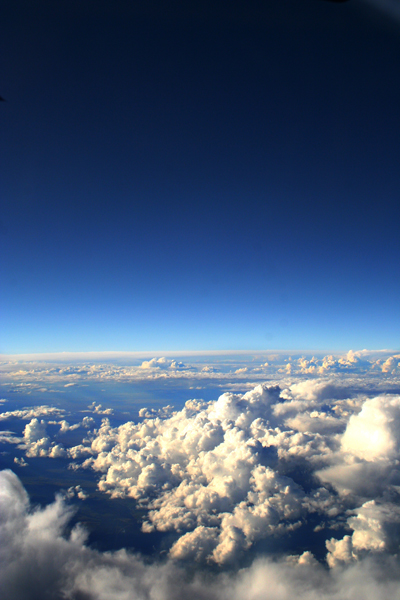
\includegraphics[width=0.4\textwidth]{Images/ceu.png}
    \caption{Imagem que ilustra o verbete “Céu” desde 2008.}
    \label{fig:ceu}
\end{figure}

Seguindo esta linha argumentativa, o ensaio conclui com as seguintes palavras: “\textit{Só porque uma coisa a si lhe parece óbvia, não significa que seja óbvia para toda a gente. Construa artigos unicamente a partir de fontes fiáveis de autoridades no assunto e cite essas fontes}” (\citewiki{ptwiki_e_preciso_citar_ceu_azul}).

Ambos os ensaios estão marcados com a predefinição ``Ensaio contestado'', que anuncia em uma caixa no topo das páginas de ambos ensaios: ``\textit{\textbf{Atenção}: Esta página contém um ensaio da Wikipédia que é seguido por parte dos seus editores, \textbf{mas é contestado por outro grupo de editores}}''\footnote{Grifos do original.} (\citewiki{ptwiki_predifinicoes_ensaios_contestado}). Ou seja, mesmo o primeiro ensaio tendo sido criado em 2011 e o segundo em 2013, até hoje, em 2020, nenhum deles foi reconhecido como uma política oficial da Wikipédia em português, e ambos contam com correligionários/as que convivem na enciclopédia com práticas antagônicas de aplicação da política de verificabilidade.

\begin{figure}[H]
    \centering
    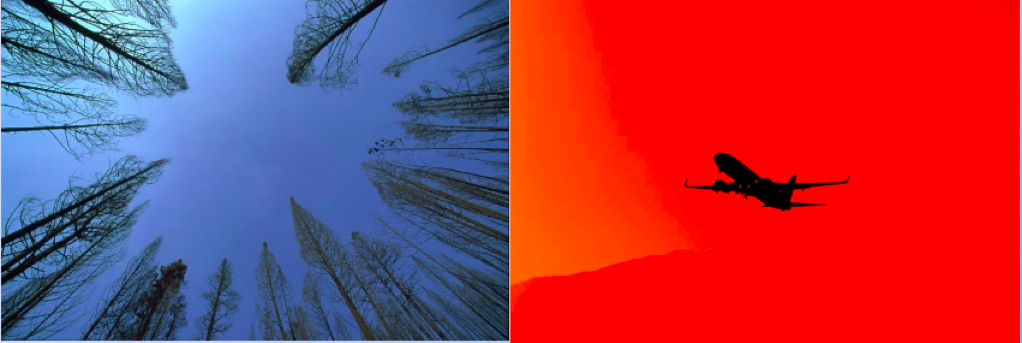
\includegraphics[width=1\textwidth]{Images/ceus-verificabilidade.png}
    \caption{Imagens que ilustram os ensaios que debatem as fronteiras de aplicação da política de verificabilidade.}
    \label{fig:ceus-verificabilidade}
\end{figure}

Situações como a relatada levaram nossa pesquisa a se interessar tanto pelos enredamentos que configuram a governança cotidiana da enciclopédia como pela forma que orientações nada triviais, como a demonstrada, podem se tornar barreiras no caminho de novos usuários que não tenha a experiência requerida para realizar devidos desvios para poderem editar.

A forma como a ambivalência de nossa pesquisa aqui citada se desenvolvera e fora implementada é então detalhada na seção a seguir.

% 
\subsection{Estudos quantitativos e a Wikipédia}

Metodologias quantitativas podem entrar em rota de colisão com os Estudos CTS, pois tendem a realizar inferências que confiam em metadados como fiéis porta-vozes dos fenômenos estudados, assim como tendem a dedicar pouca atenção às traduções\footnote{Utilizamos o termo ``tradução'' da mesma forma que  Bruno Latour, apoiados no conceito criado por Michel Serres em ``\textit{La traduction}'', de 1974, e retrabalhado em ``\textit{Le tiers-instruit}'', de 1991.}, traições, enquadramentos e transbordamentos que estão necessariamente envolvidos no processo de criação de camadas de conhecimento. Como proposto por Henrique Cukierman, em palestra no evento ``Avaliação da produção científica brasileira: pensando com a história das ciências'', organizado em 2011 pela SBHC e pelo HCTE\footnote{Sociedade Brasileira de História da Ciência (SBHC) e Programa de Pós-Graduação em História das Ciências e das Técnicas e Epistemologia da Universidade Federal do Rio de Janeiro (HCTE).}, sobre a confiança nos números, geralmente traduzida como ``objetividade'': ``\textit{O que há de especial com a linguagem da quantidade? Respondendo de forma sucinta, pode-se dizer que a quantificação é uma tecnologia de controle a distância, pouco ou nada relacionada com a chamada 'verdade' da natureza}'' (\cite[p.5]{cukierman_uma_2011}). Em seguida, citando Theodore M. Porter, ressaltou que ``\textit{a quantificação é parte de uma estratégia de intervenção, e não de mera descrição}'' (\cite[43]{porter_1996}, apud \cite[p.5]{cukierman_uma_2011}).

Na literatura de estudos sobre controvérsias na Wikipédia é comum encontrar pesquisadores/as caindo nesta armadilha da autoproclamada "objetividade" dos dados, realizando estudos profundos unicamente alicerçados em metadados que são assumidos como verdades puras e neutras, sem que os/as pesquisadores/as se ocupem em compreender como são elaborados, em observar quais ações foram de fato realizadas pelos/as usuário/as que viriam a gerar tais metadados estudados. É o caso sintetizado por Latour (\citeyear{latour_ciencia_1987}) como "\textit{o representante sendo assumido automaticamente como o representado}". 

Sigamos então com uma breve revisão bibliográfica para observar a materialidade desta prática de utilização dos metadados como porta vozes suficientes nos estudos mais citados sobre controvérsias na Wikipédia.

Em um trabalho bastante citado\footnote{89 citações segundo o Google Scholar. Página disponível em https://scholar.google.com.br/scholar?hl=pt-BR\&as\_sdt=0\%2C5\&q=Edit+wars+in+Wikipedia\&btnG= , acessada em 25 de março de 2020.}, “\textit{Edit wars in Wikipedia}”, Sumi et al (2011) propõem o índice M de controvérsia, observando “\textit{como' o número de edições e reversões desviam em algumas páginas dos números seguidos pela maioria dos artigos}”\footnote{Todas as citações desta revisão bibliográfica foram traduzidas livremente pelo autor.}. Mapeando duplas de editores/as que se revertem em um artigo e seu volume de edições no mesmo texto, os autores testam seu modelo em 6 diferentes idiomas e observam que menos de 1\% dos artigos apresentam um resultado significativo em seu índice.

O trabalho anterior foi a base do estudo ``\textit{The most controversial topics in Wikipedia: A multilingual and geographical analysis}'' de Yaseri e aliados, citado já 100 vezes por outros estudos.\footnote{https://scholar.google.com.br/scholar?hl=pt-BR\&as\_sdt=0\%2C5\&q=The+most+controversial+topics+in+Wikipedia\%3A+A+multilingual+and+geographical+analysis\&btnG= , acessada em 25 de março de 2020.} Nele foi utilizado o 
índice M como ponto de partida para observar versões em diferentes idiomas da enciclopédia buscando aproximações e similaridades entre grupos de idiomas próximos, com o objetivo explícito de criar ``\textit{um indicador multilíngue e independente da cultura}'' (\cite{yasseri_controversial_2014}). Em sua pesquisa, eles identificam que a maior parte das controvérsias são localizadas\footnote{Utilizamos ao longo desta pesquisa o termo ``localizada'' da mesma forma que o Movimento Wikimedia, adjetivando coisas que não sejam definidas globalmente pelo movimento, e podem ser instanciadas localmente de forma distinta pelas comunidades de cada projeto.}, e não se repetem tão comumente em outros idiomas (menos ainda se forem de grupos linguísticos diferentes), o que reforça a dificuldade de utilizar metadados globais para mapear comunidades com práticas distintas.

Já Vuong et al. (\citeyear{vuong_ranking_2008}), em “\textit{On ranking controversies in wikipedia: models and evaluation}”, com 115 citações\footnote{	https://scholar.google.com.br/scholar?hl=pt-BR\&as\_sdt=0\%2C5\&q=On+ranking+controversies+in+wikipedia\%3A\+models+and+evaluation\%E2\%80\%9D\&btnG= , acessada em 25 de março de 2020.}, resolvem levar em consideração não somente a atividade editorial em um artigo, como igualmente o perfil dos/as usuários/as envolvidos/as. Utilizando também a idade do artigo (em número de revisões salvas, e não em tempo corrido desde sua criação), os autores propõem diferentes índices partindo da seguinte premissa: “\textit{um/a usuário/a é mais controverso/a se participa de disputas em artigos menos controversos e um artigo é mais controverso se nele participam de disputas usuários/as menos controversos/as}”. Ambos os conceitos de controvérsia que se retroalimentam, tanto de usuários/as como de artigos, emergem de metadados brutos.

Em “\textit{There is no deadline: time evolution of Wikipedia discussions}”, o artigo menos citado desta revisão bibliográfica mas ainda assim com relevantes 32 menções\footnote{https://scholar.google.com.br/scholar?hl=pt-BR\&as\_sdt=0\%2C5\&q=There\+is+no+deadline\%3A+time+evolution+of+Wikipedia+discussions\&btnG= , acessada em 25 de março de 2020.}, Kaltenbrunner e Laniado (\citeyear{laniado_emotions_2012}) voltam-se para os metadados de edição das páginas de discussão dos artigos, onde inicialmente não encontraram padrões de volume de edições correlacionados com os metadados de suas páginas correspondentes no domínio principal. Aprofundando a inferência, criaram o indicador\textit{h}, que aponta o maior número de discussões que seja igual ao número mínimo de respostas nelas. Observando o tempo que um artigo leva para incrementar seu \textit{h}, o estudo procura “\textit{identificar escaladas ou estabilizações de controvérsias}” de forma totalmente automatizada.

Em “\textit{Visual analysis of controversy in user-generated encyclopedias}”, citado 97 vezes\footnote{	https://scholar.google.com.br/scholar?hl=pt-BR\&as\_sdt=0\%2C5\&q=Visual+analysis+of+controversy+in+user-generated+encyclopedias\&btnG= , acessada em 25 de março de 2020.}, Brandes e Lerner (\citeyear{brandes_visual_2008}) estão interessados em saber quem edita depois de quem, e qual a diferença de tempo entre essas edições. Com essas informações, o artigo cria uma visualização de usuários/as agrupados/as, simbolizando “facções” em disputas de edições. Neste caso, após gerar seus mapas a partir dos metadados, os pesquisadores buscaram ler os artigos e estudar o perfil dos/as usuários/as envolvidos/as nas disputas, tanto na versão inglesa da Wikipédia como na alemã. De forma não surpreendente para nós, após está análise qualitativa, concluíram que seu modelo tende a aproximar vândalos\footnote{Termo utilizado no Movimento Wikimedia para se referir a usuários/as que fazem edições de má fé.} e combatentes de vandalismo, pois “\textit{ambos podem apresentar o comportamento ‘um contra todos}’” (\cite{brandes_visual_2008}). Pensando em melhorias de seu trabalho que deem conta de fazer de forma automatizada tão importante distinção entre esses perfis de usuário/a tão claramente desiguais, propõem que sejam adicionados futuramente à equação mais metadados, tais como registros de bloqueios dos/as usuários/as e conversas realizadas nas páginas dos/as usuários/as.

Por fim, citamos o badalado\footnote{137 citações mapeadas no Google Scholar. Disponível em https://scholar.google.com.br/scholar?hl=pt-BR\&as\_sdt=0\%2C5\&q=Global+disease+monitoring+and+forecasting+with+Wikipedia\&btnG= , acessada em 25 de março de 2020.} trabalho “\textit{Global disease monitoring and forecasting with Wikipedia}”, de Generous et al (\citeyear{generous_global_2014}), que foi objeto de grande cobertura da mídia\footnote{Em uma rápida busca no Google ainda hoje é fácil recuperar matérias de veículos como Washington Post https://www.washingtonpost.com/news/to-your-health/wp/2014/11/13/how-wikipedia-reading-habits-can-successfully-predict-the-spread-of-disease/ , LA Times https://www.latimes.com/science/sciencenow/la-sci-sn-wikipedia-flu-disease-predictor-20141113-story.html e Revista Galileu https://revistagalileu.globo.com/Ciencia/Saude/noticia/2014/11/como-wikipedia-pode-ajudar-monitorar-doencas.html} ao buscar identificar, antes das autoridades de saúde pública, surtos de doenças epidêmicas a partir do comportamento dos/as usuários/as nas Wikipédias. Mesmo se esforçando em realizar calibragens locais, fica claro em seus resultados que enquanto muito bem-sucedidos (como alardeado pela imprensa) para algumas doenças em alguns países em um determinado recorte temporal, o modelo puramente baseado em metadados fracassou na maioria dos casos testados.

Como ficou claro, a tradição de utilizar ferramentas de ciência de dados e análise de metadados em pesquisas costuma caminhar em uma proposta metodológica antagônica à concepção CTS de abertura de caixas-pretas aqui defendida. O impasse apresentado em tentar simultaneamente acompanhar densamente dinâmicas locais e utilizar técnicas quantitativas generalizantes pode parecer então incompatível com os Estudos CTS.

Porém, nem tudo está perdido. Mesmo com alguma ressalva, Latour (\citeyear[p.167]{latour_cogitamus_2010}) relata em Cogitamus que “\textit{sim, reconheço, as ferramentas digitais são um veneno. Mas, talvez, também ofereçam um remédio. Ao menos, isso é o que exploro há dez anos com os alunos dos cursos chamados ‘mapeamento de controvérsias’. Talvez fosse possível aprender a se orientar nas disputas, com a condição de contar com uma plataforma suficientemente calibrada e padronizada, para dar a um público virtual – ainda a ser inventado – hábitos comuns}". Seguindo esta visão, podemos observar “\textit{As controvérsias da ciência na Wikipédia em português: o caso do aquecimento global}”, tese de doutorado defendida em 2014 por Bernardo Esteves. Em um grande esforço para estudar as controvérsias sobre mudanças climáticas utilizando ferramental metodológico CTS, Esteves (\citeyear[p.295]{esteves_as_2014}) observa que “\textit{na Wikipédia, cada ação dos editores deixa rastros disponíveis para consulta de pesquisadores e demais interessados, abrindo uma janela para um repositório riquíssimo de informações sobre como os usuários negociam suas versões de verdade}”, e, para dar conta desses rastros, acompanha editores/as, regras editoriais, robôs, bloqueios, discussões e proteções de páginas, narrando processos de resolução de controvérsias e de estabililização de textos enciclopédicos. Em sua pesquisa, Esteves fez tanto análises quantitativas como qualitativas, e em seus esforços de construir um olhar ao mesmo tempo amplo como o da águia e míope como o da formiga, chegou a cogitar a criação de um indicador de controvérsias que pudesse ser utilizado na Wikipédia em português imbricando estes olhares.\footnote{"\textit{Acreditamos que os resultados deste estudo poderiam ganhar mais refinamento e resolução caso tivéssemos explorado mais a fundo as ferramentas computacionais para extrair e tratar dados disponíveis na base de dados da Wikipédia. Ademais, os resultados de um tratamento estatístico mais robusto poderiam talvez contribuir para o desenvolvimento de um índice de controvérsia mais adequado às especificidades das interações ente os usuários da Wikipédia lusófona}" \cite[p.296]{esteves_as_2014}.}

Seguindo ainda outro exemplo da linha de “\textit{Mapping Controversies}” apresentada na citação acima de Latour, o Médialab do Instituto de Estudos Políticos de Paris (Science Po), o mesmo Instituto onde Bruno Latour trabalha, foi enredado com a Fundação Barcelona Media, ferramentas de visualização de dados, o DesityDesign Lab do Politécnico de Milano, metadados da Wikipédia, o Digital Methods Initiave da Universidade de Amsterdam e orçamentos de pesquisa da Comissão Europeia no Projeto Contropedia, em um esforço para “\textit{construir uma plataforma de visualização e análises em tempo real de controvérsias na Wikipédia”} (\cite{noauthor_site_2013})\footnote{Todas as citações de textos da Contropedia foram traduzidas livremente pelo autor.}. Criado em novembro de 2013, o projeto é brevemente mencionado por Esteves em sua tese, mas no momento de seu estudo praticamente não havia informações publicadas sobre o desenvolvimento do projeto. Agora, o projeto já tem resultados publicados e uma versão beta de sua plataforma disponível para uso, propondo-se a “\textit{prover um melhor entendimento de fenômenos sociotécnicos que acontecem na internet e equipar cidadãos com ferramentas para desenrolarem plenamente a complexidade de controvérsias}” \cite{noauthor_site_2013}.

Diferente dos demais estudos sobre controvérsias na Wikipédia  anteriormente citados, a Contropedia não se propões a medir quais artigos são controversos dentro de uma Wikipédia, e sim quais tópicos são controversos dentro de um determinado artigo. O índice de controvérsia da Contropedia é associado a \textit{wikilinks}\footnote{Link internos em verbetes da Wikipédia para outros verbetes dentro da enciclopédia.}, e é calculado somando edições com alguma remoção de conteúdo de frases onde o \textit{wikilink} apareça no artigo. Sendo que, caso mais de um wikilink apareça na mesma frase, o peso de controvérsia atribuído é proporcional ao número de wikilinks na frase editada \cite{borra_societal_2015}

Esse sutil deslocamento dos metadados utilizados se deve ao distanciamento do projeto dos esforços de criação de indicadores de controvérsia gerais, em direção a uma posição onde buscam apoiar quantitativamente pesquisadores/as que estejam observando detalhadamente a construção de artigos. A ferramenta se propõe então a ser um mapa que aponte indícios para pesquisadores/as que pretendam fazer investigações densas, chamando a atenção do/a pesquisador/a para tópicos dentro do artigo que ensejem um olhar mais aprofundado.

Concordamos com Erik Borra, que junto de outros pesquisadores do projeto Contropedia (\citeyear[p.196]{noauthor_site_2013}), afirma que ``\textit{reconhecer o potencial do histórico de edições da Wikipédia como provedor de insights sobre controvérsias sociais, e reconhecer que cada link em um artigo pode ser visto como um ponto focal de debate, nos permite utilizar a Wikipédia como um interessante local para mapear controvérsias}''. Esta afirmação ressona com as observações de Esteves (\citeyear[p.295]{esteves_as_2014}) segundo as quais ``\textit{até o fim do século XX, os cientistas sociais tinham que escolher entre análises quantitativas robustas que os distanciavam de seu tema de pesquisa ou análises qualitativas detalhadas que corriam o risco de perder de vista o contexto mais amplo em que seu objeto de estudo se inseria. [Os cientistas sociais] precisavam escolher entre falar muito sobre pouco ou pouco sobre muito. A difusão das ferramentas computacionais de análise de dados e a grande disponibilidade de registros deixados pelos usuários dos sistemas digitais na internet abriram novas possibilidades para as ciências sociais e tornaram viável superar ao menos em parte esse dilema}''.

É importante destacar na proposta de atuação da Contropedia a preocupação em ter a ferramenta como provocadora de insights, e não como uma instância julgadora que automaticamente decreta vereditos em nome do/a pesquisador/a. Como dito no próprio site do projeto, a ``\textit{Contropedia destaca conhecimento instável em oposição a fatos estáveis}'' (\cite{noauthor_site_2013}). Citando mais uma vez Latour, sobre a adaptação do uso de ferramentas quantitativas de ciência de dados para pesquisas CTS, “\textit{é como se houvéssemos passado da pesquisa dos matters of fact à exploração dos matters of concern”\footnote{Grifo do original.}} (\cite[p.160]{latour_cogitamus_2010}). Tomando esse ponto de vista, e tendo o devido cuidado de não buscar resolver as disputas estudadas mas orientar sua investigação, e atentando para o fato de que ``\textit{uma representação da realidade, quando transladada para um sistema de informação, é, inevitavelmente, representada em categorias sempre limitadas, previamente estabelecidas em estruturas de bancos de dados. [...] A maneira como essa classificação se dá, ou seja, a escolha das categorias para o enquadramento é uma questão importante, com efeitos para o coletivo}'' (\cite[p.8]{feitosa_cidadao_2010}), a aproximação que parecia improvável de ferramentas de análise quantitativa de dados com os Estudos CTS se torna possível.


\subsection{De dentro para fora e de fora para dentro}

A trajetória de nossa pesquisa começou em 2017, com o plano de dar sequência a um dos trabalhos futuros propostos pela tese de Bernardo Esteves\footnote{\textit{(...)os resultados deste trabalho também poderiam ser explorados com a cartografia de controvérsias, método de visualização das forças em oposição nas controvérsias proposto por pesquisadores alinhados com a Teoria Ator-Rede (\cite{venturini_diving_2010};\citeyear{venturini_building_2012}). As duas abordagens – um tratamento estatístico de maior escopo e a visualização com a cartografia de controvérsias – são duas perspectivas possíveis de desdobramento deste trabalho no futuro em parceria com outros pesquisadores.}" (\cite[p.296]{esteves_as_2014})} e investigar ferramentas de mapeamento e cartografia de controvérsias na Wikipédia. Em nosso esforço inaugural neste caminho foi produzido um primeiro artigo, ``\textit{Controvérsias na Wikipédia lusófona: pode o olhar CTS ser apoiado por ferramentas quantitativas?}'', apresentado no \textit{International Wikipedia Scientific Conference} (IWSC), que se propôs a ``\textit{revisar esforços prévios de mapeamentos de controvérsias na Wikipédia e analisar o funcionamento da ferramenta Contropedia, explicitando suas funcionalidades e a utilizando para observar algumas controvérsias, a fim de entender como ferramentas quantitativas podem apoiar estudos de controvérsias que utilizem abordagens CTS}'' (\cite[p.1]{de_andrade_controversias_2017}).

Após este primeiro resultado de nosso projeto de pesquisa, passamos a estudar \textit{in loco} diferentes práticas de escrita na Wikipédia, suas barreiras e resultados obtidos, com ênfase em possíveis peculiaridades da Wikipédia em português. 

Esta nova abordagem se materializou em uma apresentação feita no 6º Simpósio Nacional de Ciência, Tecnologia e Sociedade (ESOCITE.BR), intitulada “\textit{Histórias das ciências para todos: uma prática de escrita biográfica na Wikipédia em português}”, onde é “\textit{lançado um olhar CTS sobre a escrita de conteúdos enciclopédicos relacionados aos estudos de Ciências-Tecnologias-Sociedades, descrevendo três cenas de edição da Wikipédia acontecidas no contexto de uma disciplina de pós-graduação, cada qual com objetivos, enredamentos, desvios, alistamentos e resultados bem distintos}” (\cite{andrade_historias_2017}).

No desenvolvimento das duas abordagens de pesquisa abertas foi possível observar que o onipresente discurso de que “\textit{todos podem editar}” não se mostrava na prática tão óbvio como colocado pela comunidade, e o interesse por sua exploração passou então a figurar como tema central da investigação que segue. Este movimento se soma a leitura da dissertação “\textit{O discurso do global nas comunidades de software livre: estudo de caso do WordPress}”, defendida por Rodrigo Primo no Programa de Engenheria de Sistemas e Computação da COPPE/UFRJ, em 2017, na qual problematiza o discurso de adesão e representatividade global da comunidade que desenvolve o Wordpress, CMS\footnote{Do inglês Content management system, são sistemas de publicação e gerenciamento de páginas online.} mais utilizado do mundo. Sua problematização é construída a partir do estudo das dinâmicas de funcionamento e organização interna do Wordpress. Percebemos então que nosso estudo não deveria se ocupar diretamente das controvérsias presentes na escrita de verbetes, e sim nas controvérsias predecessoras a estas, onde políticas editoriais, regras de atuação e sistemas automatizados são interessados\footnote{Utilizamos na pesquisa o termo ``interessar'' da mesma forma que Callon, significando a prática de enredar actantes de forma que os mantenham como aliados estáveis.} (\cite{callon_scallops_1986}) e posteriormente ``caixapretados''.

Assim, inspirados pelos caminhos trilhados pelos dois trabalhos apresentados, percebemos que a investigação proposta precisaria ser trilhada por duas abordagens de pesquisa distintas, uma que chamaremos ``de dentro para fora'' (ADENTROF) e a outra ``de fora para dentro'' (AFORAD).

Na abordagem ``de dentro para fora'', seguimos usuários/as experientes envolvidos/as na governança da enciclopédia e em seus/suas processos de decisão e ação, a fim de observar a materialidade das práticas que dão gênese aos metadados tão utilizados pelos/as estudiosos/as de controvérsias aqui já citados/as. São apresentados aos leitores detalhes do fazer da governança da Wikipédia em português, passando por: seus processos de criação de regras; suas estratégias para garantir seu padrão de qualidade; seu software MediaWiki e seus filtros de edição, captchas e listas brancas e negras; sua relação com as comunidades globais e sua gestão dos servidores.

Já a abordagem ``de fora para dentro'' segue editores/as recém-chegados/as à prática de escrita wikipédica, e as barreiras enfrentadas por eles/as, enquanto tentam colaborar com a comunidade. Nesta abordagem da pesquisa são mapeadas traduções e negociações feitas para tornar o conteúdo dos/as novatos/as aceitável pela comunidade. Esta abordagem da pesquisa observa o histórico das atividades de \textit{outreach} do Movimento Wikimedia, como o Programa de Educação, as parceiras GLAM\footnote{Sigla em inglês para "\textit{Galleries, Libraries, Archives \& Museums}", usada pelo movimento para se referir a projetos feitos em parceria com galerias, bibliotecas, arquivos e museus.} e as maratonas de edição, focando seus esforços nessa última categoria de atividades. Por fim, realizamos nossas próprias editatonas, podendo assim seguirmos bem de perto as dinâmicas vivenciadas por usuários/as novatos/as participando destas atividades editando a Wikipédia.

Ambas as abordagens foram apoiadas tanto por uma abordagem quantitativa, através da utilização de softwares que acessam os bancos de dados abertos da enciclopédia e analisam padrões e comportamentos, como também por pesquisas de campo, através de leituras de históricos de discussão e entrevistas com editores/as experientes administradores/as da Wikipédia.

Para garantir a exequibilidade desta pesquisa, muitos elementos interessantes transbordaram para fora do quadro, pois, como nos ensina Callon (\citeyear[18]{callon_markets_1998}), ``qualquer enquadramento é necessariamente sujeito ao transbordamento''. Ao caminhar da pesquisa, escolhas foram necessariamente feitas para definir recortes em zonas cinzentas em torno de nossas bordas. Todavia, ao longo do texto existe a preocupação de apontar os movimentos em que definições claras de enquadramentos se fizeram necessárias. Desta forma, a presente pesquisa não somente se mantém leal à sua metodologia, como situa o/a leitor/a no caminho trilhado, propiciando não apenas uma leitura contextualizada e honesta, como também facilitando passos de futuros/as pesquisadores/as que venham a não só replicar os experimentos e inferências desta pesquisa como também dos que se cativem por pesquisar a Wikipédia com diferentes enquadramentos, em busca de análises distintas das aqui apresentadas.





%capítulo 2: de dentro para fora
\chapter{De dentro para fora}

\singlespacing
\begin{flushright}
\textit{``A toda hora,}

\textit{a todo momento}

\textit{De dentro pra fora}

\textit{...''}

Walter Franco
\end{flushright}
\doublespacing

Na abordagem ``de dentro para fora'', nossa pesquisa segue usuários experientes envolvidos na governança da enciclopédia e de seus processos de decisão e ação, aproximando-nos da materialidade das práticas que geram os metadados tão utilizados já prontos pelos estudiosos de controvérsias na Wikipédia. Serão apresentados ao leitor detalhes do fazer da governança da Wikipédia em português, passando por seus processos de criação de regras, suas estratégias para garantir seu padrão de qualidade, seu software MediaWiki e seus filtros de edição, captchas e listas brancas e negras e sua relação com as comunidades globais.

Esta frente de pesquisa foi apoiada tanto por uma abordagem quantitativa, através da utilização de softwares que acessam os bancos de dados abertos da enciclopédia e analisam padrões e comportamentos, como também por pesquisas de campo, através de leituras de históricos de discussão e entrevistas com editores experientes administradores da Wikipédia.

%\section{Era uma vez uma enciclopédia colaborativa}

A origem da Wikipédia e a tradição enciclopedista já foram contadas diversas vezes e de diferentes formas por vários pesquisadores, e neste trabalho não nos propomos a refazer estes esforços.\footnote{Ao leitor que desejar se aprofundar na origem do enciclopedismo, recomendamos a leitura do capítulo "O enciclopedismo de Plínio a Jimmy Wales, em (\cite{esteves_as_2014}).} Em nossa análise nos interessamos pelo movimento presente do fazer da Wikipédia que, segundo Jankowski (\citeyear{jankowski_wikipedia_2013}), é caraterizada pela colaboração, co-construção, cooperação, confiança na comunidade e construcionismo, em oposição à tradição enciclopedista, que se baseia nos valores epistêmicos de utilitarismo, organização sistêmica, autoridade, confiança em especialistas e consistência.

Esta diferenciação de valores pode ser vista como uma ruptura que se sustenta a partir da ``\textit{produção colaborativa feita por editores voluntários. Não há um projeto norteando seu desenvolvimento. Os artigos são criados e dimensionados conforme o desígnio dos colaboradores (...). Ela parece romper, portanto, com o modelo de produção de conteúdo confiada a especialistas, predominante no enciclopedismo pelo menos desde a Encyclopédie}''  \citep[p.61]{esteves_as_2014}. Segundo Demo (\citeyear{demo_conhecimento_2009}), essa ``\textit{conclamação à sociedade em geral para produzir conhecimento}'' é algo nunca antes visto, pois ``\textit{produzir conhecimento sempre foi atividade reservada, preservada, censurada (Shattuck, 1996. Rescher, 1987), tendo como patrulheiros os especialistas e as entidades que os abrigavam.}'' \citep{demo_conhecimento_2009}.

A conclamação apresenta resultados visíveis em números: hoje, a auto-intitulada ``\textit{enciclopédia livre, que qualquer um pode editar}'' é o décimo site mais visitado do mundo \citep{alexa_2019}, contando com enciclopédias em 303 idiomas diferentes. Cabe destacar que, ainda que traduções sejam permitidas, cada enciclopédia tem sua escrita feita de forma independente  \citewiki{ptwiki_sobre} com políticas editoriais e regras de convivência que podem variar de acordo com as comunidades locais. \citep{marques_wikipedia_2013}. Ao final de 2019, suas 303 versões diferentes somadas apresentavam cifras impressionantes: mais de 40 milhões de verbetes, 400 mil editores ativos por mês e 500 milhões de visitantes únicos também por mês. \citep{wikimedia_stats_2019}

Em meio a tantos verbetes, visitantes e editores, é interessante notar a dificuldade da Wikipédia em se definir. Buscando sua identidade, a comunidade prefere usar a negação do que a afirmação. Em momentos de ruptura e conflito, aparenta ser mais fácil falar o que não se é do que o que se é. Tal movimento não é novidade, e pode ser encontrado por exemplo na fala de Tião Rocha, relatada em Severo (\citeyear[p. 19-20]{severo_tics_2016}): ``\textit{Tião tirou do chapéu-cartola a seguinte matreirice: \textbf{os não-objetivos} da educação. Ele escreveu um documento, similar a um manifesto, onde estava \textbf{listado tudo aquilo que aquele grupo não queria} que acontecesse com os filhos dos outros em uma escola (...) o nosso compromisso é: se nós não fizermos o que está listado nessa folha, o resto é lucro}''.\footnote{Grifos nossos.}

Tal qual uma pintura onde a figura é revelada a partir da construção do fundo, na página ``\textit{O que a Wikipédia não é}'' a comunidade lusófona pinta seus transbordamentos apresentando 20 seções textuais, cada uma dedicada a versar sobre algo que deve estar fora de seu enquadramento. Começando por não ser uma ``\textit{enciclopédia impressa}'', deixando claro no caminho ``\textit{não ser um consultório médico}'' nem ``\textit{um campo de batalha}'', e concluindo com a afirmação de que ``\textit{não é uma sociedade secreta}''. \citewiki{ptwiki_naoe}.

A construção de ``o que a Wikipédia não é'' mobiliza muito mais a comunidade do que dizer para o mundo afirmativamente o que ela é. A página “Sobre a Wikipédia”, primeiro link visto por um usuário que acesse a página principal da Wikipédia em português, tem um conteúdo bem mais tímido que sua contraparte negacionista,  contando com quatro seções que totalizam 5.889 bytes, desenvolvidos em 215 edições feitas por 134 editores distintos 
\footnote{Dados encontrados em https://xtools.wmflabs.org/articleinfo/pt.wikipedia.org/Wikipédia:Sobre\_a\_Wikipédia?uselang=pt-br , acessada em 11 de abril de 2020.}. Já a página sobre seus transbordamentos é mais que cinco vezes maior, com 33.503 bytes trabalhados em 412 edições por 149 diferentes editores. 
\footnote{Dados encontrados em https://xtools.wmflabs.org/articleinfo/pt.wikipedia.org/Wikipédia:O\_que\_a\_Wikipédia\_não\_é?uselang=pt-br , acessada em 11 de abril de 2020.} 

Pesquisar uma comunidade que tem dificuldades em dizer o que é tráz claramente dificuldades e desafios. Em nossos esforços de realizar análises quantitativas coladas aos bancos de dados, precisamos criar recortes e métricas que, ao descrever o que está sendo estudado, também o prescreve e, portanto, nossas escolhas podem apontar para definições do que ``a Wikipédia é'' que não sejam consensuais.

Apresentando um exemplo concreto, trabalhamos na pesquisa com recortes de usuários tanto por grupos de tipo de permissão de acesso ao MediaWiki como por atividades em diferentes espaços da enciclopédia. A relevância tanto dos estatutos \footnote{Estatuto é como a comunidade se refere às permissões que um usuário ganha ao fazer parte de um grupo de usuários no MediaWiki.} como dos espaços de participação escolhidos como representativos pela pesquisa desta dissertação pode ser reafirmada ou deslegitimada, a depender do que se entenda afinal ser a Wikipédia e suas comunidades.

O termo ``comunidades'' aliás é muito utilizado no mundo da Wikipédia e sua abrangência varia bastante de acordo com o escopo tratado. Por exemplo, a ``comunidade de wikipedistas'' engloba todos os atores pelo mundo que atuam em alguma Wikipédia. Já o termo ``comunidade lusófona'' irá se referir apenas aos que participam da Wikipédia em português. Assim, cada projeto\footnote{Projeto" é a forma como as comunidades se referenciam a cada instância wiki distinta.} tem sua comunidade que é a autora de seus conteúdos e gestora de sua governança, dentro dos limites permitidos pelo Movimento Wikimedia.\footnote{O Movimento Wikimedia nasceu da expansão da Wikipédia, que em busca de realizar seu objetivo principal enunciado como ``Imagine um mundo onde cada pessoa do planeta tenha acesso livre a soma de todo conhecimento da humanidade. É isso que estamos fazendo'' decidiu ao longo do tempo criar outros projetos de construção coletiva de conhecimento para abarcar conteúdos que segundo as políticas editoriais não seriam considerados enciclopédicos. Assim nascem Wikcionário, Wikilivros, Wikinotícias, Wikivoyage e diversas outras wikis com suas próprias comunidades, não necessariamente interessadas na construção enciclopédias. Assim, o Movimento Wikimedia passa a ser entendido como a união das comunidades de todos esses projetos (e também das comunidades de desenvolvedores de softwares de/para wikis, que detalharemos posteriormente) e cabe a ele, através da Fundação Wikimedia, definir regras gerais que devem ser seguidas por todos os projetos.}

A compreensão do que é ou não uma Wikipédia varia ao longo de suas diversas comunidades, e pode encontrar consensos locais que não sejam globais. A própria página “O que não é a Wikipédia”, se observada em outros idiomas, terá algumas seções em comum e outras divergentes. Enquanto a versão em português conta com 20 tópicos, suas correlatas apresentam 19 tópicos em inglês, 22 em francês, 14 em espanhol e 9 itens em alemão.\footnote{ \citewiki{enwiki_isnot}; \citewiki{frwiki_nest}; \citewiki{eswiki_noes}; \citewiki{dewiki_nichtist}}. 

Não avançamos na diferença entre os conteúdos destas páginas pois em nossa pesquisa preferimos trabalhar com as definições que se constituem na prática cotidiana das comunidades. Observamos então a configuração das comunidades ditada a partir da prática wikipédica de produção coletiva de conteúdos, seguindo suas dinâmicas e especificidades.

\subsection{A escrita wikipédica}

Inspirada abertamente pelo movimento software livre desde sua fundação \citep{lih_wikirevolution_2009}, a Wikipédia se distancia da prática de escrita tradicional enciclopédica ao ter sua política editorial centrada em escritores não-especialistas e em coautoria massiva. Tomando emprestado o termo de Tião Rocha apud (\cite{severo_tics_2016}), esse ``\textit{empodimento}''\footnote{Versão localizada do termo em inglês \textit{empowerment}} é uma característica que distancia o fazer da Wikipédia da prática de escrita científica, tradicionalmente exercida por um autor solitário, o especialista, ou com poucos coautores.

Ao estudar a prática de historiadores, Rosenzweig (\citeyear{rosenzweig_can_2006}) diz existir um individualismo possessivo na produção de conteúdos, e atenta para o fato de ser considerada uma boa prática na área sempre citar o nome do autor quando for se referir a uma ideia, mesmo que esteja sendo lateralmente mencionada e já seja consensual entre os interlocutores. Complementando que ``\textit{um trabalho de história sem donos, ou com múltiplos donos anônimos, é algo inimaginável em nossa prática profissional.}''\footnote{Tradução livre do original em inglês: ``A historical work without owners and with multiple, anonymous authors is thus almost unimaginable in our professional culture.''} 

Nesta mesma toada caminha a ciência como um todo em seus textos. Como nos ensina a também historiadora Juliana Marques, ``\textit{na academia supõe-se como condição sine qua non que haja um ou mais autores para determinado texto, responsáveis pelo conteúdo e que tenham uma qualificação mínima reconhecida por seus pares para que se justifique a autoridade de sua argumentação. São proprietários do texto na sua forma total, e a reapropriação, fragmentação e modificação deste sem prévia autorização constitui plágio, reconhecido legalmente como crime}''. \citep[337]{marques_trabalhando_2012}

A escrita coletiva feita por anônimos permite observar colaborações na construção de conteúdos de forma estável por certo tempo, e, assim como o fazer da ciência, a escrita da Wikipédia segue um ``\textit{caminho muito estranho porque é invisível quando tudo vai bem}'' \citep[p.44]{latour_cogitamus_2010}. Porém, no contínuo exercício de escrita e revisão das edições feitas entre usuários, como seria de se esperar, divergências e controvérsias emergem, quebrando o moto contínuo de estabilidade editorial e demandando desvios, que ensejam novas abordagens, formas de agir, regras e ferramentas tecnológicas. São estes casos, onde acontecem enredamentos de diferentes elementos em busca de novas estabilizações, que exploraremos para entender o funcionamento prático da enciclopédia.

Um dos movimentos mais exemplares deste enredamento de novos elementos para estabilização de controvérsias é a busca por aliados que sustentem um determinado texto. Curiosamente, apesar das diferenças entre as práticas de escrita wikipédica e científica apontadas acima, a busca por aliados mais poderosos para reforçar uma posição é tão similar em ambos processos de escrita que a seguinte passagem de Latour (\citeyear[p.48]{latour_cogitamus_2010}), originalmente sobre textos científicos, poderia muito bem versar sobre a Wikipédia: ``\textit{A presença ou ausência de referências, citações e notas de rodapé é um sinal tão importante de que o documento é ou não sério que um fato pode ser transformado em ficção ou uma ficção em fato apenas com o acréscimo ou a subtração de referências}''.

Esta dança literária, praticada por editores e textos em busca de um lugar ao sol na maior enciclopédia do mundo, acontece em páginas públicas, onde todas as mensagens, controvérsias e históricos de alteração estão acessíveis a qualquer leitor. Porém, o fato de estar lá disponível não significa que na prática a grande maioria dos leitores acesse estes espaços.

No mesmo movimento da ciência que exibe uma face pronta e outra ainda em construção, ilustrado por Latour (\citeyear{latour_ciencia_1987}) através duas faces de Jano bifronte, a Wikipédia também tem suas duas faces distintas. Enquanto uma, conhecida do grande público, apresenta textos grandes, ilustrados e referenciados, a outra é incerta, instável, está em constante movimento para ganhar uma forma estável e é conhecida por poucos.

\begin{figure}[H]
    \centering
    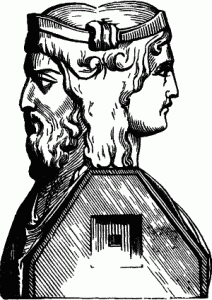
\includegraphics[width=0.5\textwidth]{Images/duas_faces_jano.png}
    \caption{As duas faces de Jano bifronte.}
    \label{fig:duas_faces_jano}
\end{figure}

É esta segunda face, sempre em construção e distante das vistas da grande audiência, que expressa a criação das regras e dinâmicas que interessam à investigação proposta neste capítulo. Seguindo os traços deste rosto encontramos acirradas disputas sobre qualidade editorial, grupos de usuários atuando em funções administrativas, robôs e demais elementos que serão explorados nas seções a seguir.

\subsection{Busca por qualidade}

Enquanto milhões de pessoas acessam diariamente a maior enciclopédia do mundo, uma rede de elementos heterogêneos está 24 horas se movimentando para garantir a estabilidade do que é apresentado. Uma rede de atores humanos e não-humanos (usuários, robôs, fundações, filtros, referências, métricas, ferramentas, políticas editoriais ...) faz o trabalho pesado semi invisível para que a maioria dos leitores desinteressados possam apenas enxergar textos e figuras estabilizados.

Em meio a essa incessante busca por garantir a qualidade dos conteúdos apresentados, no processo de proteger a enciclopédia de edições danosas é recorrente que usuários novatos, ainda não familiarizados com as políticas editoriais da enciclopédia, sejam tratados como vândalos\footnote{O termo ``vandalismo'' neste contexto se refere a edições de má fé feitas na Wikipédia.} \citep{halfaker_snuggle:_2014}. Este problema é habitual motivo de debates em vários espaços de discussão da Wikipédia, como o Projeto AntiVandalismo\footnote{Portal disponível em https://pt.wikipedia.org/wiki/Wikipédia:Projetos/AntiVandalismo .}, com usuários buscando estratégias para combater o vandalismo sem ``jogar fora o bebê junto com a água do banho''.

Na busca por formas de separar novatos bem-vindos na comunidade daqueles que se deseja afastar já foram propostas diversas iniciativas, desde mudanças comportamentais de editores patrulhadores à utilização de ferramentas automatizadas, que vão do uso de filtros de edições e captchas\footnote{Captcha, ``\textit{Completely Automated Public Turing test to tell Computers and Humans Apart}'', é uma funcionalidade presente em vários sistemas que intenta descobrir se o usuário é um humano ou um robô.} no MediaWiki a robôs que realizam reversões e enviam boas-vindas \citep{halfaker_bots_2012} e modelos de aprendizado de máquina (também chamados de inteligências artificiais) que predizem se edições foram feitas em boa fé, se são potencialmente danosas e se devem ser revertidas. \citep{halfaker_artificial_2015}

Todos esses esforços buscam realizar traduções de desejos de actantes distintos das comunidades, interessando políticas editoriais, softwares, editores e demais elementos em torno de iniciativas que visem atender interesses comuns, mesmo que temporariamente. Cabe relembrar que, conforme explicado no capítulo anterior, neste trabalho entendemos tradução como definido por Bruno Latour no livro Cogitamus (\citeyear[p.30]{latour_cogitamus_2010}): ``\textit{traduzir é ao mesmo tempo transcrever, transpor, deslocar, transferir e, portanto, transportar transformando}'', tendo sempre em mente que ``\textit{toda tradução implica uma traição, dado que, invariavelmente, um conceito, artefato ou máquina, quando trazido para outra situação histórica, é adaptado, reinventado na prática, renegociado, para que funcione conforme as novas condições e ambiente.}'' (\cite[p.27]{feitosa_cidadao_2010})

Este processo de tradução é muito claro e visível na esperança wikipédica de que as massas anônimas negociem regras e práticas, chegando sempre a um resultado de composição mais interessante do que a ação isolada e independente.

A expectativa quase determinística desta profecia de garantia de qualidade pode ser bem observada na descrição feita por Pedro Demo (\citeyear{demo_conhecimento_2009}), de que ``\textit{do caos pode provir ordem, como sugere Holland, em processo de criatividade crescente, ainda que a natureza, em si, nada ‘crie’ do nada. Ela cria do que já existe, ou seja, reconstrói indefinidamente. Esta expectativa faz parte da construção da wikipedia, referenciada também como ‘efeito-piranha’ ou ‘stigmergy’, categorias da pesquisa biológica para descrever o comportamento de vespas e cupins, quando constroem coletivamente estruturas complexas; o produto do trabalho prévio, ao invés de comunicação direta entre os construtores, induz e direciona como tais insetos realizam trabalho adicional e sem comando central de cima para baixo. Ocorreria algo similar na Wikipédia: cada editor retoma o trabalho anterior e assume aí um direcionamento para continuar, redundando, ao final, num texto aprimorado}''.

Seguindo a lógica da citada esperança, a Wikipédia tem como base de sua política de qualidade a Lei de Linus, cunhada por Eric Raymond ao estudar comunidades de software livre, que diz ``\textit{dados olhos suficientes qualquer problema é trivial}'' (\citeyear{raymond_cathedral_1999}) \footnote{Tradução livre. No original em inglês ``\textit{Given enough eyeballs, all bugs are shallow}''.}. Nos primórdios da Wikipédia, a referida ``lei'' pode ter sido analogamente bem a aplicada a ela. Porém, atualmente, com uma média maior a 7.000 edições por dia\footnote{Dados do segundo semestre de 2019 disponíveis em http://stats.wikimedia.org , visitado em 15/04/2020} apenas na Wikipédia lusófona, volume de contribuições muito maior do que qualquer comunidade de software jamais viu, a comunidade de enciclopedistas virtuais não consegue ter olhos suficientes verificando a qualidade de todas edições feitas. 

No ímpeto de garantir a tão almejada qualidade em meio tal volume massivo de edições, usuários ativos criam traduções que não enredam todos usuários, deixando diversos editores de fora de seu enquadramento de contribuidores de qualidade. Conforme cresce a audiência, os esforços despendidos para manter estável a qualidade da Wikipédia parecem conflitar com seus princípios de abertura e sua política de que ``qualquer um pode editar''.

Assim, em meio a páginas de mudanças recentes, patrulhadores, filtros de edição, ferramentas semi automatizadas e robôs reversores, uma boa parte das edições feitas é revertida\footnote{Termo utilizado pelos wikipedistas para se referir a ação de restaurar uma versão anterior da página, descartando as contribuições mais recentes.}, e os autores das contribuições rejeitadas costumam receber mensagens padronizadas,  que vão desde um texto informando que sua edição ``\textit{não parece ser construtiva e teve de ser revertida}'' o convidando a utilizar ``\textit{a página de testes para fazer testes de edição à vontade sem danificar a Wikipédia}'' \citewiki{ptwiki_avisovandalismo} até um aviso de que foram bloqueados, parcial ou totalmente, do site \citewiki{ptwiki_politica_bloqueio}.

Este aparente conflito entre a ``qualidade'' e a ``abertura'' da Wikipédia foi objeto de uma pesquisa encomendada pela Wikimedia Foundation em 2010 aos pesquisadores Robert Harris and Dory Carr-Harris, intitulada ``\textit{Wikimedia Study of Controversial Content}'', onde foram apresentadas propostas de como a comunidade deveria lidar com tópicos ``controversos''. No escopo do estudo, ``controverso'' é entendido como algo que ``\textit{implica um processo social, um reconhecimento de que um conteúdo possa gerar uma reação em largos grupos de indivíduos, de forma independente, e sem motivação ulterior}'' \citep{harris_2010_2010}. Em outras palavras, está sendo pautado na pesquisa ``o que pode ser editado?'', com os pesquisadores estudando tanto o histórico de ``\textit{compromisso com abertura intelectual}'' da Wikipédia como seu objetivo de ser um ``\textit{empreendimento educacional que sirva a todos os cidadãos do mundo}'', apontando possíveis conflitos entre uma abertura total e irrestrita na produção e a preocupação em oferecer um material educacional que seja percebido como de qualidade e lido por todos os povos do planeta.

Ao final do estudo são propostas algumas detalhadas políticas de como as comunidades Wikimedia deveriam atuar para estabelecer as fronteiras dos territórios da qualidade e da abertura. Porém, como poderíamos imaginar, as propostas criadas por observadores externos não lograram consenso junto às comunidades, fomentando discussões que se seguiram em diversos fóruns wikipédicos.

Um dos espaços para onde a discussão transborda é o \textit{The Signpost}, ``jornal'' feito pela e para a comunidade da Wikipédia em inglês, publicado mensalmente com média superior a 7 mil leitores por edição.\footnote{Dados obtidos em https://tools.wmflabs.org/pageviews/?project=en.wikipedia.org\&platform=all-access\&agent=user\&redirects=0\&start=2019-04\&end=2020-03\&pages=Wikipedia:Wikipedia\_Signpost , acessada em 22 de abril de 2020.} Nos comentários de uma entrevista com Sue Gardner publicada no The Signpost de janeiro de 2012 \citewiki{enwiki_signpost}, um dos jornalistas responsáveis  pela entrevista, apesar da ressalva feita por ele mesmo de que talvez não devesse se engajar no debate exatamente por ter conduzido a entrevista, ``troca de chapéu'' e entra como wikipedista na controvérsia que se desenrola nos comentários. Tony1, usuário registrado desde 2005, na época com mais de 70 mil edições feitas (hoje passa de 200 mil)\footnote{Dados disponíveis em  https://xtools.wmflabs.org/ec/en.wikipedia.org/Tony1, acessada em 31 de março de 2020.}, faz um resgate histórico e fala sobre as duas forças antagônicas objetos do estudo:

``\textit{Nos velhos tempos, a qualidade e a abrangência dos artigos eram enojantes, mas não nos importávamos muito: prevalecia uma mentalidade fronteiriça e não precisávamos competir tão intensamente por nossa reputação na internet. As coisas começaram a ficar mais sérias a partir de 2005 e, durante o processo, alguns artigos que professores universitários ridicularizavam gradualmente se tornaram melhor escritos do que os que eles próprios eram capazes de produzir. Nos tornamos mais sujeitos a regras (como todas as publicações de qualidade) e mais exigentes com todos os editores. De fato, nos afastamos de 'qualquer um pode editar' e devemos aceitar como inevitável que a aplicação da qualidade tenha tornado a Wikipédia menos 'acolhedora' para os novatos, muitos dos quais carecem de habilidades e paciência para aprender os padrões exigidos para esse produto cultural. \textbf{Abertura e qualidade são, portanto, colocadas umas contra as outras em aspectos-chave.}}''\footnote{Tradução livre do original em inglês: ``\textit{Back in the early days, article quality and comprehensiveness were queasy, but we didn't care that much: a frontier mentality prevailed and we didn't have to compete quite so keenly for our reputation on the internet. Things started getting more serious from about 2005 onwards, and in the process, some articles that university lecturers might have once scoffed at gradually became better written than they themselves are capable of producing. We became more rule-bound (like all quality publications) and more demanding of all editors. In effect, we pulled away from "anyone can edit", and we should accept as inevitable that quality enforcement has made WP less "welcoming" to newcomers, many of whom lack the skills and patience to learn the patterns demanded of this cultural product. Openness and quality are thus pitted against each other in key respects}''.} \citewiki{enwiki_talk_signpost}\footnote{Grifos nossos.}

O que para Tony1 é um movimento que torna a Wikipédia ``\textit{menos acolhedora para os novatos}'', para outros pode ser visto como um movimento que cerceia a liberdade de expressão fundadora do projeto. Como dito pelo professor Pedro Demo (\citeyear{demo_conhecimento_2009}), ``\textit{as promessas de liberdade de expressão foram, aos poucos, sendo restringidas, em parte por causa de seus abusos (o preço da liberdade é seu abuso), em parte para organizar melhor o processo produtivo e garantir padrões mínimos de qualidade acadêmica. A rebeldia do conhecimento se submeteu crescentemente a ritos de enquadramento, sugerindo que a wikipedia também expressa ambigüidades comuns a projetos coletivos que se querem libertários: forjados para captar e potencializar a contribuição livre de todos, somente avançam e se consolidam sob crescente regulação da participação, das atividades e das instituições. O exercício coletivo da liberdade implica seu cerceamento, em nome do bem comum}''.

Seguindo este movimento de busca por qualidade e enrijecimento de regras (que potencialmente gera cerceamento do exercício de liberdades) encontramos a política de verificabilidade. Ela sustenta que, tal qual um trabalho científico, toda afirmação publicada na Wikipédia deva ser referenciada e verificável. Seguindo a tradição enciclopédica, isso significa que se está criando um compêndio de conhecimento através do ``\textit{esforço de 'compilação' do que existe. Tomado isto ao pé da letra, segue que seu conteúdo é típico 'remix', ou, reinterpretação das interpretações, discurso de discursos. Não caberia pesquisa original, a não ser se fosse já algo compilado.}'' \citep{demo_conhecimento_2009}.

Se diferenciando de outras enciclopédias, a Wikipédia preconiza ser uma fonte terciária de informações, buscando sempre utilizar em suas referências fontes secundárias. Desta forma, não somente a pesquisa original estará fora do escopo do trabalho do enciclopedista, como também resta terceirizada a validação da qualidade destes trabalhos originais, que é confiada às fontes secundárias.


\begin{figure}[H]
    \centering
    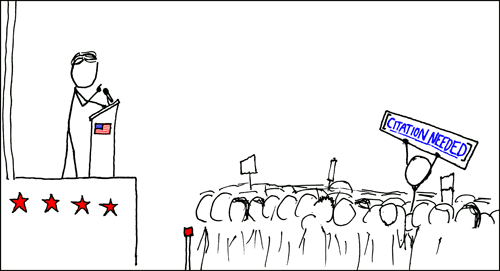
\includegraphics[width=1\textwidth]{Images/tirinha_randall_munroe.png}
    \caption{Tirinha de Randall Munroe que ilustra a página ``Wikipedia:Citation needed'', na Wikipédia anglófona com a seguinte legenda: ``A predefinição \{\{Carece de fontes\}\} visa promover discursos responsabilizáveis.'' \citewiki{enwiki_citation_needed}}
    \label{fig:tirinha_randall_munroe}
\end{figure}
\footnotetext{No original ``\textit{The \{\{Citation needed\}\} template aims to promote accountable discourse}''.}

Percebe-se então uma mudança crítica no trabalho do enciclopedista. Ao decidir se uma informação deve ter lugar em sua publicação, ele passa a ter sua atenção deslocada da preocupação com a ``veracidade'', para os conceitos complementares de ``verificabilidade'' e ``fiabilidade''.

Com isso, as principais discussões editoriais na Wikipédia são focadas na presença e na confiabilidade de fontes, e não diretamente na veracidade dos conteúdos individualizados. Ao contrário do que possa parecer a um primeiro olhar, este movimento não remove o especialista da cadeia de produção de conteúdo, mas apenas o desloca. Como explica Esteves (\citeyear[p.62]{esteves_as_2014}), ``\textit{Os especialistas continuam presentes, mas nas referências que devem fundamentar cada informação inserida nos artigos}". Assim, não é esperado que o especialista se apresente pessoalmente para os embates dentro da Wikipédia, mas que esse trabalho seja feito por porta-vozes seus. Um porta-voz, como bem sintetizado por Latour (\citeyear[p.108]{latour_ciencia_1987}),  ``\textit{é alguém que fala em lugar do que não fala. [...] um representante que expresse seus interesses, que fale em nome deles}''.

Dentro das disputas editoriais wikipédicas, os editores então terão maior chance de sucesso em seus argumentos e defesas de acordo com a reputação e o prestígio das vozes que estiver portando em seu discurso. Pois ``\textit{estar diante de um porta-voz não é o mesmo que estar diante de qualquer homem ou mulher comum. Não se está diante de Bill ou do Professor, mas diante de Bill, do Professor e mais as muitas coisas ou pessoas no interesse das quais eles estão falando}''. (\citep[p. 109]{latour_ciencia_1987}) Assim, ``\textit{longe de se livrar da autoridade do especialista, a Wikipédia depositou confiança nela}''\citep[p. 121]{jankowski_wikipedia_2013}.

É interessante notar que a participação dos porta-vozes não é algo que aconteça pela mera falta do especialista, e que tenderia a se diluir caso mais doutos se engajassem na escrita da enciclopédia colaborativa. A representação indireta através de porta-vozes é não só esperada como desejada pela comunidade, que entende esta terceirização como uma de suas inúmeras formas de garantir qualidade em sua produção editorial. Entende-se que o autor de uma pesquisa possa estar muito apegado a sua visão enviesada\footnote{No inglês ``\textit{biased}'', termo muito utilizado em debates no movimento Wikimedia sobre ``neutralidade''.} de um determinado assunto e tenda a apresentar conflito de interesses na escrita, pois se beneficiaria pessoal e diretamente de ter sua produção citada por um verbete da maior enciclopédia do mundo. \citewiki{ptwiki_conflito_interesses}

Seguindo esta linha de raciocínio, o editor não especialista, que atua traduzindo o conhecimento produzido por um autor (fonte primária) e já validado por uma entidade respeitada socialmente, sejam pares, jornalistas ou corpos editoriais (fonte secundária), terá maior traquejo para se movimentar entre diferentes abordagens de um mesmo tema, sendo a figura mais indicada para escrever um verbete enciclopédico de forma ``neutra''.\footnote{Ao longo do trabalho optamos por sempre escrever termos como ``neutro'' e ``neutralidade'' entre aspas para reforçar que são conceitos utilizados pela comunidade, mas não corroborados por este estudo.}

Esse movimento em busca de uma suposta ``neutralidade'' gera um curioso dualismo. Por um lado ele se sustenta necessariamente em uma crítica epistemológica à ciência moderna ocidental, que não teria em seus representantes o mero papel de reveladores de verdades naturais. Pois, é dito que se a eles fosse estimulado escrever diretamente os textos enciclopédicos relacionados a suas pesquisas, os verbetes acabariam maculados por interesses e política. Por outro lado, a busca por um texto enciclopédico neutro sugestiona que os wikipedistas, ao contrário dos cientistas, seriam sim capazes de escrever uma história de fatos e artefatos desprovida de subjetividades e enviesamentos.

``\textit{A contradição é flagrante e claramente sarcástica: de um lado, se todos podem editar, isto representaria naturalmente a diversidade de pontos de vista; de outro, espera-se que tudo isso se acalme num texto final de um único ponto de vista; no entanto, se todos podem editar sempre, não haveria texto final, mas em progresso incessante; nem se poderia imaginar que os textos, oriundos de incontáveis pontos vista, acabassem como peças sem ponto de vista (...) NPOV\footnote{Do inglês ``\textit{Neutral Point Of View}'', como é conhecida a política de neutralidade na Wikipédia.} aparece na cena como excrescência, um alinhamento a metodologias positivistas e que em nada funciona neste tipo de ambiente. É farsa cômoda.}'' \citep{demo_conhecimento_2009}

Mas, esse dualismo não parece ser uma grande questão para a maior parte da comunidade. A ``neutralidade'' em sua escrita é um dos pilares do Movimento Wikimedia \citewiki{ptwiki_cinco_pilares}, e usuários que tentam o questionar ou relativizar tender a ser rechaçados (a página "Wikipédia:Princípio da imparcialidade", que detalha a aplicação deste pilar, é linkada em mais de 250 mil outras páginas)\footnote{Dados disponiveis em https://xtools.wmflabs.org/articleinfo/pt.wikipedia.org/Wikipédia:Princípio\_da\_imparcialidade , acessado em 16 de junho de 2020.}. Ao mesmo tempo, é facilmente identificável no cotidiano da escrita wikipédica a utilização de fontes secundárias pouco conhecidas como referências para sustentação de afirmações, sem que seja realizado um escrutínio da suposta ``neutralidade'' de cada fonte. 

Assim, enquanto no discurso wikipédico da neutralidade pode ser facilmente identificada a presunção positivista enciclopédica da criação de um compêndio objetivo de todo o conhecimento humano \citep{esteves_as_2014}, o mesmo discurso não se apresenta tão estabilizado e inquestionável como o cientificismo positivista, e vê sua política editorial ser constantemente atacada por defensores do rigor científico. \citep{taraborelli_expert_2011} O protagonismo de não especialistas e a possibilidade de utilizar como fontes materiais produzidos por não cientistas coloca, para seus críticos, a Wikipédia em um local de produção de conteúdos não confiáveis.

Nos aproximamos assim de algo que pode ser visto como um paradoxo. A Wikipédia depõe a ciência do papel de um mero agente neutro revelador de verdades naturais. Mas, ao contrário do que poderíamos esperar, ao invés de com este movimento de destronamento da ciência, a comunidade buscar se sustentar em novas epistemologias não determinísticas de construção de verdades, a enciclopédia opta por se vender como o autêntico grande catalisador de verdades neutralizadas globais.

Essa curiosa situação paradoxal se propaga por todos os desdobramentos da defesa do modelo de produção colaborativa wiki e de sua suposta garantia de qualidade. Sua política explícita de utilização de fontes secundárias ``fiáveis'', simplesmente dá transparência à mesma dinâmica que estrutura o funcionamento de todas as ciências.

Seguindo esta linha de raciocínio, pode-se afirmar que essa transparência na construção de verdades acende um holofote sobre a fragilidade do argumento da existência de uma ``verdade una natural descoberta''. Com isso, para a Wikipédia ser ``verdadeira'' ou até mais confiável que outras enciclopédias, seria coerente que ela adotasse uma diferente visão da construção de fatos e artefatos diferente desta denunciada tradicional positivista.

Afinal, se é possível aos wikipedistas construírem uma verdade ``neutra'', como podem acusar os cientistas de não terem a mesma capacidade de criá-la e, ao mesmo tempo, utilizarem suas (dos cientistas) produções supostamente enviesadas como fontes de sustentação de sua (da Wikipédia) produção ``neutra''? 

\begin{figure}[H]
    \centering
    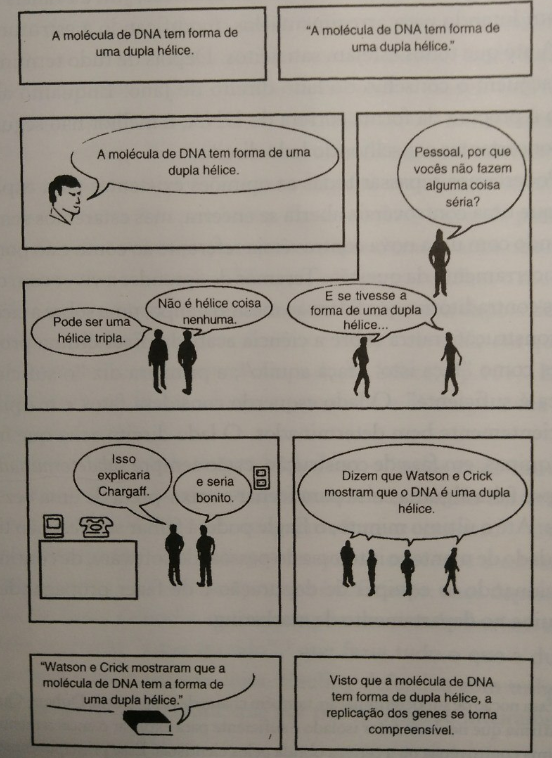
\includegraphics[width=0.5\textwidth]{Images/livro_ciencia_em_acao.png}
    \caption{Figura 1.6 do livro Ciência em Ação de Bruno Latour (\citeyear[p. 22]{latour_ciencia_1987}).}
    \label{fig:livro_ciencia_em_acao}
\end{figure}

Mas, mesmo perante esse aparente paradoxo, a escrita wikipédica apresenta algumas características que a diferenciam da escrita científica na estailibização de fatos. Na figura acima, retirada do livro Ciência em Ação de Bruno Latour, o último quadro onde ``\textit{vemos uma nova frase, sem aspas, escrita num livro}'' \citep[p.23]{latour_ciencia_1987} poderia muito bem ser a Wikipédia, só que desta vez a frase teria um pequeno número ao lado, indicando a referência que a sustenta. Em uma visão da ciência historicizada, como apresentada na figura, a transparência que a Wikipédia oferece ao leitor para saber onde dar o próximo passo, se desejar puxar o fio do novelo que levou à estabilização do fato ali apresentado, seria vista como um grande diferencial de qualidade se comparada com livros tradicionais que apresentam ``\textit{uma nova frase, sem aspas}'', como apontado por Latour.

``\textit{Inicialmente pelo menos, a Wikipédia tinha esta visão de seus textos: em progresso infindável, sem formato final, aberto à reconstrução de todos sem peias. Este estilo de 'fundamento sem fundo' (Demo, 2008) elabora uma expectativa dialética da produção de conhecimento que contrasta ostensivamente com outras inseridas na wikipedia de teor modernista e positivista, tal qual a noção de enciclopédia como guarda do conhecimento disponível, ou de neutralidade de sua produção pelos contribuintes, ou de verificabilidade dos conteúdos dos textos. A noção de conhecimento como dinâmica desconstrutiva/reconstrutiva é traída aí em nome de um estilo estabilizado, congelado e definitivo que já se poderia 'preservar'.}'' (\citeyear{demo_conhecimento_2009})

O discurso wikipedista de sempre dar transparência à procedência de suas afirmações é muito potente, e inclusive diversas vezes é apontado em palestras e apresentações como seu diferencial de qualidade perante outras produções. Porém, ao se apegar a citada ``\textit{expectativa dialética de teor modernista e positivista}'', a Wikipédia esvazia uma visão de mundo onde verdades não são reveladas, mas sim construídas, e se expõe mais fragilmente a críticas comumente vindas de setores ligados à academia e professores, que defendem com unhas e dentes que seus estudantes consultem livros (que seriam sempre confiáveis pois imutáveis) ao invés da Wikipédia (que não seria confiável pois ``qualquer um pode editar'').

Cabe aqui nos debruçarmos um pouco mais sobre o estranho duplipensar praticado por quem acusa a Wikipédia de não ser confiável mas ao mesmo tempo crê acriticamente em livros sem investigar a história de cada um individualmente. Qual seria afinal a garantia de qualidade de um livro impresso? A prensa teria por acaso algum compromisso moral com a verdade? Essa irônica pergunta nem sentido faz em nossa visão metodológica, pois já compreendemos que o processo de ``escrever verdades'' não é uma mera descrição de uma natureza revelada. Porém, apenas como exercício retórico, podemos brevemente assumir que essa visão naturalizada da construção de fatos e artefatos seja verdadeira. Assim, nossa pergunta deixa de ser mero despeito e ironia e se torna um questionamento relevante: como afinal impressoras mundo afora garantem que não estão sendo impressas mentiras? 

Perante a impossibilidade de encontrar uma resposta positiva para a pergunta, só nos resta concluir que a autoridade do livro é uma mera tradição/construção cultural/mercadológica, que aparenta não se sustentar nem mesmo no modelo conservador de verdades estanques reveladas, se feitas as perguntas certas. Aqui por honestidade intelectual, nos cabe observar que, como bem já disse algum antigo sábio português, ``pau que dá em Chico também dá em Francisco''. Ao desconstruirmos a autoridade emanada dos livros também estamos apontando o dedo para a Wikipédia. Pois afinal, esta utiliza os primeiros como fonte para seus textos. Por coerência metodológica, devemos então observar os efeitos de tal implicação para a escrita wikipédica. 

A grande diferença, inclusive autoproclamada como vantagem, do modelo de produção de conteúdo enciclopedista wiki para a tradicional escrita literária, está na intensa discussão sobre a fiabilidade de suas fontes. Livros \textit{per se} não são considerados fontes fiáveis pela Wikipédia. Para serem aceitos como dignos de credibilidade, não basta palavras terem sido convertidas em tinta bem recebida pelo papel. Seus autores e corpos editoriais precisam ter reputações e reconhecimentos que sejam entendidos como relevantes pela comunidade, para então serem acreditados como fontes fiáveis.

Seguindo o fio desta reflexão, é quase inevitável encontrar a curiosa conclusão de que a principal crítica feita à qualidade da Wikipédia (de que qualquer um pode editar), se apontada para o modelo dito tradicional de produção de conhecimento (o mesmo exaltado pelos críticos da metodologia wiki), revelará uma enorme probabilidade de ``mentiras'' serem propagadas através de livros, revistas, apostilas e manuais. Pois, afinal, hoje em dia ``qualquer um pode editar um livro''.

Enquanto isso, ironicamente, o modelo wiki apresenta regras que se preocupam em mitigar esse risco, oferecendo ao hesitante leitor formas razoavelmente transparentes de rastrear a validação feita por terceiros das informações ali apresentadas, propiciando assim maior enredamento e, por consequência, robustez aos textos ali publicados.
%\section{MediaWiki: o juiz dos casos invisíveis}

Partimos nesta seção para a abertura de caixas-pretas da criação de regras na Wikipédia, com especial atenção para aquelas que, uma vez implementadas, passam a ter sua execução automatizada. Elementos como filtros de edição, listas brancas e negras e ferramentas automatizadas de avaliação de qualidade de edições foram estudados. Levantamos dados sobre cada uma delas, entendendo sua importância no funcionamento da comunidade e estudando suas origens e estabilizações.

Nos interessou nesta investigação especialmente entender como regras são naturalizadas e viram coisas acima de qualquer suspeita, ``que obviamente sempre estiveram ali''. Entendemos que para proceder com esta investigação é preciso entender a macro estrutura onde estas regras são criadas, assim como o ``campo de batalha'' onde são disputadas e as peças que se movem (ou se mantém estáticas) neste tabuleiro.

Também é mister entender o arcabouço tecnológico vigente que, apesar de passar longe de ser determinístico para definir regras \textit{a priori}, atua como um importante ator que sempre participa das negociações, podendo através de suas facilidades e/ou complexidades apresentar argumentos fortíssimos em favor de determinadas regras e/ou desabonadores de outras.

Optamos então por seguir regras que de alguma forma tem sua implementação embedada em código-fonte no software que media a operação das Wikipédias, o MediaWiki, estudando não somente suas origens e estabilizações, como também seus resultados práticos e volumes de interação (que podem ser traduzidas como criações de barreiras) com os enciclopedistas.

O MediaWiki é o território virtual onde os wikipedistas vivem. O sistema de gestão de plataformas wikis, criado e mantido pela própria comunidade Wikimedia, organiza e sistematiza não só as formas como os conteúdos são exibidos como também as dinâmicas de interação e organização das comunidades que o utilizam.

A utilização massiva do MediaWiki é muito cara à comunidade Wikimedia, que não vê com bons olhos a utilização de outras ferramentas de gestão de tarefas ou de comunicação, buscando sempre estimular que a ferramenta seja utilizada para tudo que for possível.

Em seus primórdios, a Wikipédia utilizava outra ferramenta para gestão de suas wikis, o UseModWiki \citep{lih_wikirevolution_2009}. Mas, dado seu crescimento e a demanda por atendimento a uma escala de visitas maior que qualquer outra wiki do planeta, somada a anseios cada vez maiores por customizações do sistema para suas dinâmicas, a comunidade, liderada pelo voluntário Magnus Manske, resolve desenvolver seu próprio sistema gestor de wikis e cria uma comunidade independente dedicada ao desenvolvimento do software.

Desde então, o Movimento Wikimedia estabeleceu diversos outros projetos de criação de conteúdos educacionais, mas até hoje o MediaWiki é o único projeto oficial do Movimento Wikimedia cujo produto final é um software.

A necessidade de habilidades específicas para escrita de código-fonte para o MediaWiki torna este projeto diferente dos demais, onde (nos demais) editores podem transitar com maior facilidade. Considerando que a maioria dos wikimedistas não são programadores, o projeto  MediaWiki acaba criando uma comunidade dentro do movimento Wikimedia mais restrita e menos acessível para participantes de outros projetos.

Não obstante ser um projeto irmão da enciclopédia e ter seu código-fonte aberto, o MediaWiki é estabilizado na operação diária da Wikipédia como uma caixa-preta. Sua atuação cotidiana assim se torna invisível, e somente seus \textit{outputs} são levados em conta. Exatamente como previsto por Bruno Latour, a comunidade somente se atenta para a forma como a caixa-preta funciona em momentos de pane que bloqueem a operação padrão rotineira. Apenas quando se fazem necessários desvios de rota e angariamentos de novas composições que a caixa-preta do MediaWiki é aberta, dissecada, questionada e posta a prova, conforme veremos mais detalhadamente nas próximas seções.

Mesmo os usuários não programadores, apesar de não ``viverem'' o dia-a-dia da comunidade MediaWiki, são agentes que estão sempre negociando com este software a operação diária das Wikipédias. É fácil notar como muitas vezes discussões sobre mudanças de regras passam por questionamentos como ``\textit{dá para fazer isso no MediaWiki?}'' ou ``\textit{algum voluntário programador poderia fazer aquilo?}''. O sistema é um ator ativo na construção da governança das Wikipédias, que muitas vezes se mostra intransigente em seus posicionamentos e delimita fronteiras de atuação. Assim, acaba fornecendo a seus porta-vozes um grande poder, os autorizando a decretar ``inviabilidade técnica'' de determinadas propostas quando oportuno.

Além de sua atuação na negociação de confecção de regras, inúmeras vezes cabe ao MediaWiki ser o papel de ser o responsável por garantir o cumprimento das mesmas. Visando ``ganharem tempo'' para realizar tarefas percebidas como mais nobres ou prazenteiras, wikipedistas delegam para o software várias tarefas ditas óbvias de controle do que pode ser editado na Wikipédia. Na prática, o MediaWiki atua como uma ``barreira de primeiro nível'' extremamente confiável, bloqueando e filtrando edições que ``obviamente'' não deveriam ser salvas, sem ter sua atuação escrutinada corriqueiramente por nenhum outro ator.

Diferente das regras que são fiscalizadas e aplicadas por usuários, sejam humanos ou robôs, que deixam rastros digitais claros em espaços frequentemente visitados pela comunidade (como a página de ``Mudanças Recentes''), as ações tomadas pelo MediaWiki são logadas em espaços mais obscuros de seu banco de dados, conhecidos apenas por um pequeno número de programadores.

Enquanto as demais regras, que estão a todo tempo exibindo os resultados práticos de sua aplicação para os wikipedistas, acabam de tempos em tempos sendo questionadas e rediscutidas, o mesmo raramente acontece com aquelas que estão programadas no MediaWiki.

Acreditamos que, exatamente por estarem implementadas em códigos-fontes automatizados, as regras aplicadas pelo MediaWiki acabam ganhando o status de inquestionáveis, e passam despercebidas mesmo por usuários mais aguerridos em todos os debates ligados a governança do projeto. Afinal, não se pode questionar o que não se vê.

Com isso, podemos falar que o MediaWiki se porta como o grande juiz dos casos invisíveis da Wikipédia. Ou, em outras palavras, que o software atua como uma rede que consolida uma caixa-preta. Entendendo que ``\textit{tem-se uma caixa-preta quando muitos elementos são levados a atuar como um só}'' \citep[205]{latour_ciencia_1987}, e seguindo o interesse desta pesquisa em abrir caixas-pretas, partimos então nas próximas páginas a observar quais elementos configuram esta rede e realizam traduções que permitem sua estabilização.

Assim como todo software gestor de conteúdos, o MediaWiki media as interações e ao mesmo tempo direciona os caminhos dos usuários na plataforma. Dentre as dezenas de atividades performadas por ele, elegemos enquadrar em nossa pesquisa três grupos de funcionalidades que podem explicitar com riqueza esse movimento de tradução de interesses e estabilização de uma caixa-preta, pois atuam diretamente com questões sempre presentes em discussões sobre regras editoriais e tem sua calibragem definida por regras estabelecidas por usuários. São elas: ``lista branca e lista negra'', ``filtros de edição'' e ``CAPTCHA''.

\subsection{Lista Negra e Lista Branca}

Segundo a própria Wikipédia, uma ``lista negra'' é uma lista ``\textit{que, por alguma razão, nega certos direitos, serviços, participação ou mobilidade a alguém ou a alguma entidade, em determinada situação, período de tempo ou lugar}''. \citewiki{ptwiki_lista_negra_definicao}\footnote{Termos como ``branca'' e ``negra'' são utilizados aqui conforme encontrados no campo, e não faz parte do escopo de nossa pesquisa investigar reflexões no comportamento de usuários que percebam racismo no linguajar utilizado pela comunidade.}

Ainda segundo a Wikipédia, ``\textit{em informática, usa-se o termo lista negra ( ou Blacklist (em inglês) ) para designar uma lista de e-mails, endereços IP ou até mesmo domínios, que identificam fontes de spam. \textit{Freqüentemente} torna-se útil esse auxílio com o intuito de restringir todos os elementos de uma rede que inspiram desconfiança de spam}''.

Dentro das Wikipédias, as listas negras existem ``\textit{principalmente para controlar o spam generalizado e a perturbação dos projetos da Wikimedia Foundation}''. \citewiki{ptwiki_lista_negra}

Segundo a regra sobre a utilização de ``Ligações externas''\footnote{Não muito utilizada neste contexto no Brasil, a palavra "ligação" aqui significa um \textit{link} para uma página web.} para outros sites, existem três tipos de links que são proibidos na Wikipédia em português: (1) links com códigos de marketing de afiliados, (2) links para conteúdos com violação de direito autoral e (3) ``\textit{websites que façam parte da lista de spam local ou global sem que tenham sido whitelisted}''. Diferente das duas primeiras proibições, esta terceira é complementada com a seguinte afirmação: ``\textbf{\textit{O código MediaWiki bloqueia automaticamente quaisquer edições com essas ligações}}''. \citewiki{ptwiki_ligacoes_externas_ligacoes_proibidas}

Cabe explicar que o termo ``\textit{whitelisted}'' da citação acima deve ser entendido como ``colocado na lista branca''. Lista esta que funciona como uma coletânea de exceções às listas negras. A lista negra então pode ser vista como a lista principal, onde domínios\footnote{Domínio aqui é usado para falar sobre a base dos endereços utilizados para encontrar servidores na internet, e normalmente contêm diversas páginas em suas estruturas. Se traduzido para o inglês, seria utilizada a palavra ``\textit{domain}''. Não confundir com ditos em português ``domínios'' internos da Wikipédia, que em inglês são chamados de ``\textit{namespaces}''.} são bloqueados. Já a lista branca tenderá a conter páginas específicas que podem ser liberadas em domínios indesejados (ou domínios inteiros que se deseje liberar em projeto e estejam bloqueados na lista negra global).

Sempre que uma edição é salva em um projeto Wikimedia, o MediaWiki varre duas listas negras verificando todos os links externos adicionados. Uma lista é mantida pela comunidade local (como a Wikipédia em português), e a outra pela comunidade global. Caso o software encontre o domínio da URL de um dos links adicionados em uma das listas negras, ele então busca por exceções na lista branca local.

Caso não encontre uma exceção que se aplique ao link desejado, é exibido ao usuário um aviso informando que ``\textit{não foi possível salvar (Gravar) a página devido ao bloqueio do filtro de spam}'', com um link para a página com mais informações sobre o ``\textit{filtro de spam da Wikipédia}'' \citewiki{ptwiki_mediawiki_spam_blacklist_info}.

\begin{figure}[H]
    \centering
    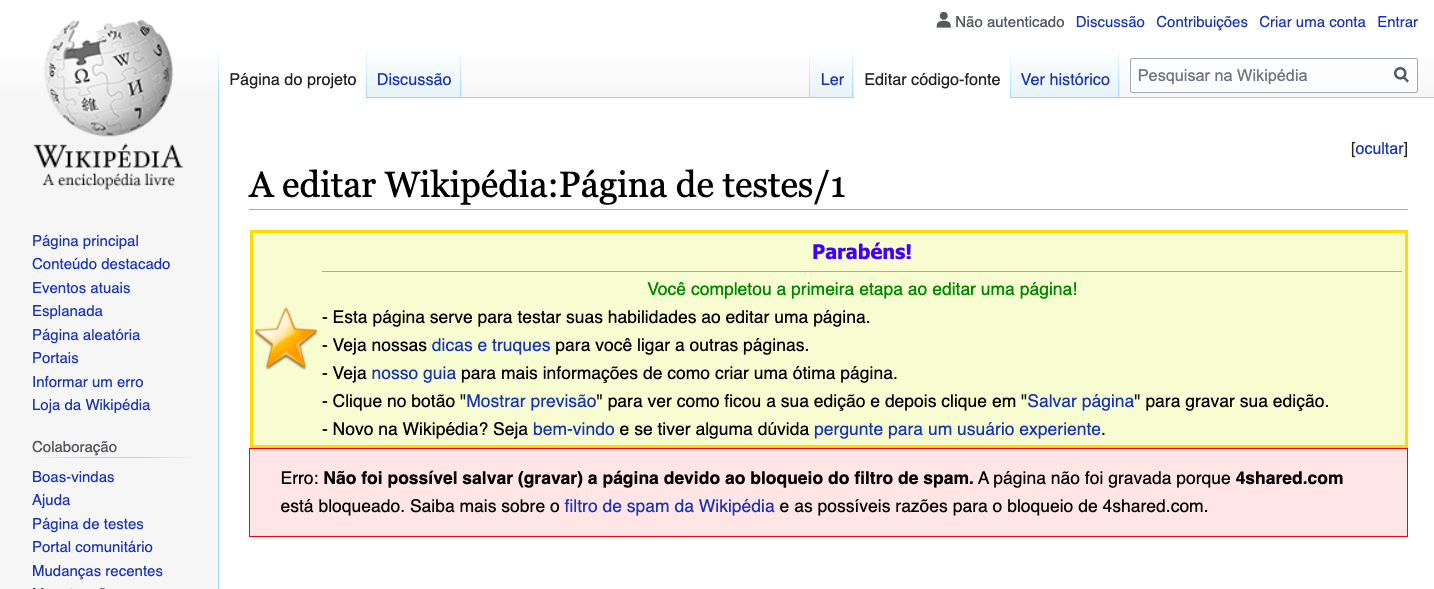
\includegraphics[width=1\textwidth]{Images/mediawiki_blacklist.png}
    \caption{Na caixa vermelha pode ser vista a mensagem que o MediaWiki exibe ao proibir uma edição que adicionaria um link para uma página listada na blacklist.}
    \label{fig:mediawiki_blacklist}
\end{figure}

Ao final desta página, é informado ao usuário que ``\textit{caso você acredite que um endereço não deveria estar bloqueado, é possível solicitar uma exceção para esta página em particular ou o desbloqueio do site}'', com links internos para as páginas onde as solicitações podem ser feitas.

Todas as discussões de bloqueio ou desbloqueio de links devem ser feitas em páginas wikis do projeto local. Buscando organizar suas páginas administrativas, muitas vezes as comunidades criam \textit{templates} que devem ser utilizados em pedidos para padronizar a forma como são apresentados. No caso do link citado no parágrafo anterior, o usuário não somente será encaminhado para a página de discussão da ``Spam-whitelist'', como o bloco de edição já aparecerá preenchido com o \textit{template}, conforme pode ser visto na figura:

\begin{figure}[H]
    \centering
    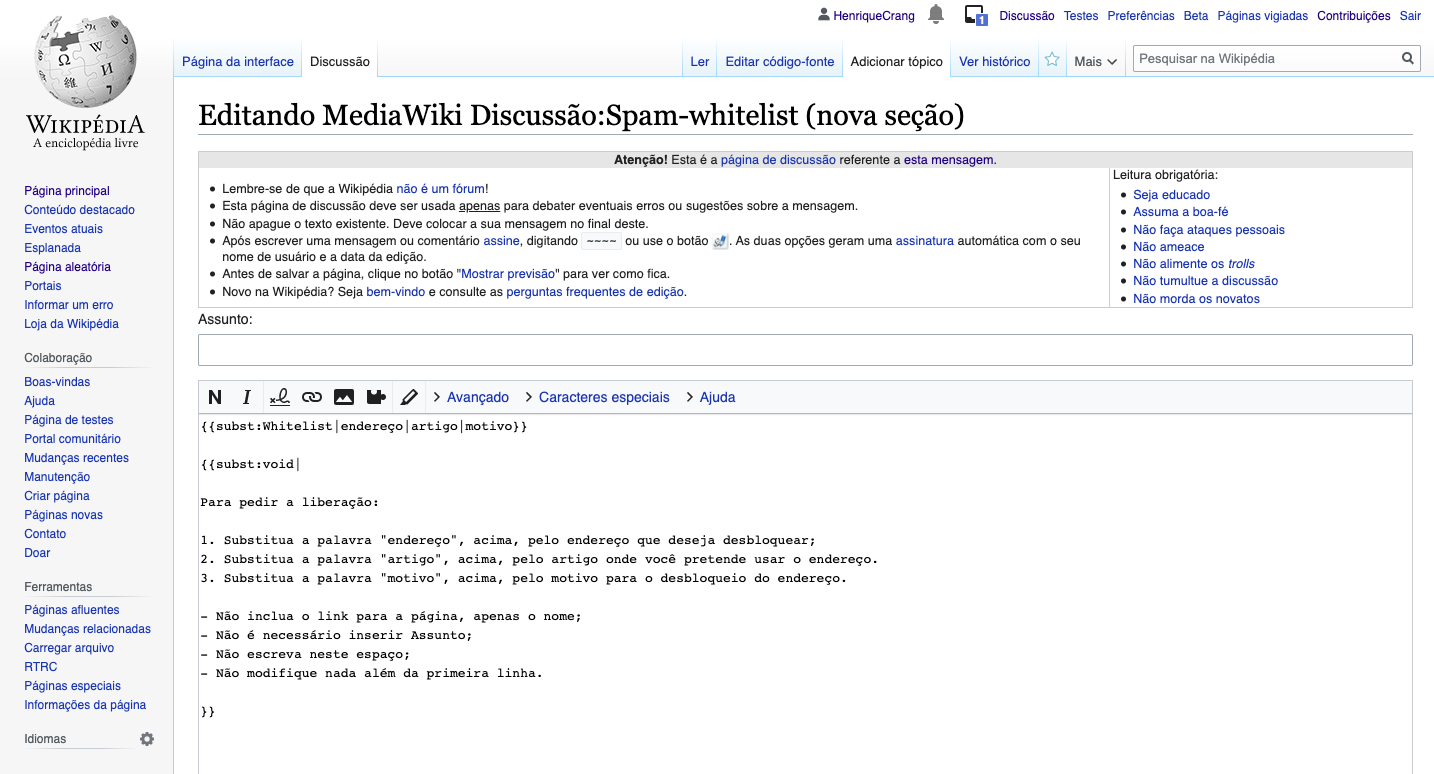
\includegraphics[width=1\textwidth]{Images/mediawiki_spam_whitelist.png}
    \caption{Página que é exibida quando um usuário clica no link interno para solicitar uma exceção à lista negra.}
    \label{fig:mediawiki_spam_whitelist}
\end{figure}

Essa estrutura de \textit{templates} é muito conhecida pela comunidade e sua utilização é fluida para wikipedistas experientes, mas é comum usuários novatos não entenderem as instruções ali contidas e preencherem o \textit{template} nos locais errados e/ou não desenvolverem no espaço reservado para o ``motivo'' da solicitação os argumentos esperados pelos wikipedistas, levando a diversos pedidos serem negados sem que pudessem ser devidamente compreendidos. \citewiki{ptwiki_mediawiki_discussao_spam_whitelist}

Além da dificuldade no uso do template, também não é trivial para editores recém chegados a diferença entre ``pedir para um endereço ser adicionado à whitelist'' (que deve ser usado para solicitar exceções para uma página específica dentro de um domínio proibido) e ``pedir para um endereço ser removido da blacklist'' (que deve ser usado para liberar um domínio inteiro). Como dito pelo administrador Edmond Dantès em resposta a um pedido de exceção na lista branca, ``\textit{Não liberamos domínios}'' \citewiki{ptwiki_mediawiki_discussao_spam_whitelist}. Caso um usuário deseje retirar um domínio inteiro da lista negra, a comunidade espera que ele se dirija a outro local: a página de discussão ``MediaWiki:Spam-blacklist'' \citewiki{ptwiki_mediawiki_discussao_spam_blacklist}.

Esta página ``MediaWiki:Spam-blacklist'', onde fica a lista de sites bloqueados, já foi editada 3275 vezes, enquanto a página ``MediaWiki:Spam-whitelist'', onde o MediaWiki encontra a lista de exceções,  apresenta 276 alterações. (\cite{quarry_edit_mediawiki_namespace}).\footnote{Todas as referências feitas à HenriqueCrang apontam para as queries realizadas nos bancos de dados do movimento Wikimedia durante a pesquisa. Ao final do trabalho, podem ser encontrados links para elas, com seus resultados e códigos-fontes.} Já suas respectivas páginas de discussão, onde os pedidos são feitos, não apresentam a mesma desproporção. 2347 edições foram feitas na página com pedidos de adição de sites na lista negra, enquanto 3208 edições foram realizadas na discussão sobre a lista branca (\cite{quarry_edit_mediawiki_talk_namespace}). Essa grande diferença na proporção entre edições na página de discussão e na página principal sugere que boa parte dos pedidos de bloqueio feitos são implementados, enquanto a maioria dos pedidos de exceções são negados.

Todas as edições na página de discussão da \textit{blacklist} foram feitas por apenas 166 usuários, sendo que só 37 deles fizeram mais de dez edições cada. (\cite{quarry_edit_sbl_talk_page}) Já nas discussões de exceções, encontramos a participação de 659 usuários distintos (\cite{quarry_edit_swl_talk_page}), mas com um número ainda menor de usuários fazendo mais que dez edições: 27.

Esses números sugerem que a discussão sobre \textit{blacklist} tende a ser mais concentrada, com usuários experientes que a conhecem debatendo quais sites devem ser bloqueados, enquanto a lista branca (talvez inclusive por ser linkada na mensagem de bloqueio conforme visto na figura anterior), atrai um número maior de usuários não tão engajados em a acompanhar, provavelmente interessados apenas em seu pedido específico.

Seguindo o rastro desta hipótese, encontramos 380 usuários com uma única edição na discussão da whitelist (\cite{quarry_only_1edit_swl_talk_page}), enquanto sua contraparte negra conta apenas com 44 editores nesta situação (\cite{quarry_only_1edit_sbl_talk_page}). Esses números claramente demonstram que as páginas tem dinâmicas de participação bem distintas, com usuários não engajados na confecção das regras claramente mais preocupados em tentar liberar determinado tipo de edição do que em proibir.

Após todas essas edições, hoje a \textit{Blacklist} da Wikipédia em português apresenta mais de 3000 domínios proibidos de serem linkados, que se somam as mais de 11 mil entradas na lista de Spam Global do Movimento Wikimedia. \citewiki{enwiki_wikimedia_spam_blacklist} Cabe destacar que muitas destas entradas são feitas utilizando expressões regulares \footnote{Expressões regulares, ou \textit{regex}, são uma forma de representar cadeias de caracteres que devam ser identificados por uma determinada função.} que podem bloquear diversos domínios de uma vez, tornando impossível precisarmos o número total de domínios proibidos. Já a lista de exceções da Wikipédia em português apresenta um tamanho muito mais humilde, com 117 endereços especificados.

\subsubsection{Deslocamentos e aumento de escopo}

Apesar de criadas para combater a ação de \textit{spammers}, com o passar do tempo a comunidade passou a delegar também às listas negras do MediaWiki a tarefa de impedir edições que adicionem links para domínios que sejam considerados inapropriados como referências para os verbetes, como hoje pode ser lido na própria página com mais informações sobre o funcionamento da Spam-blacklist: ``\textit{Por decisão da comunidade, alguns sites são considerados fontes não-confiáveis e são bloqueados para evitar sua utilização em artigos}'' \citewiki{ptwiki_mediawiki_spam_blacklist_info}.

Esta nova utilidade da ferramenta não se estabilizou sem controvérsias. Como podemos observar em uma discussão acontecida na Esplanada \footnote{A Esplanada é uma página interna da Wikipédia em português que funciona como um fórum geral, onde editores podem compartilhar e debater notícias, ideias e propostas.} em 2012 \citewiki{ptwiki_esplanada_geral_spam_blacklist}, quando o usuário Braswiki chamou a atenção da comunidade para a prática que estava se tornando habitual e perguntou: ``\textit{a lista negra de spam deve servir para impedir a inclusão de fontes não fiáveis ou apenas se esses sites estiverem sendo utilizadas como spam?}''

Nesta discussão encontramos a fala do usuário Desempates, que demonstra preocupação com o uso ``deturpado'' da ferramenta que deveria coibir spam: ``\textit{Um problema que noto é que está havendo uma deturpação dos objetivos originais da lista. Como o próprio nome indica, uma Spam-blacklist, visaria exclusivamente o bloqueio de sites de spammers. Para os demais casos, como a falta de fiabilidade, seria mais adequado que houvesse uma outra listagem}''. Sua fala é reforçada pela posição de Helder, que comenta ``\textit{a MediaWiki:Spam-blacklist deve ser usada para impedir SPAM, isto é, propaganda \textbf{em massa}, não propagandas em circunstâncias isoladas, como as feitas por um único editor ou em um único artigo, muito menos para fazer  ‘controle de qualidade’ das ligações externas.}'' (grifo do original), destacando ainda em seu posicionamento os resultados de uma pesquisa realizada pela WMF em 2011, que apontava para o volume de edições na blacklist lusófona ser maior que o dobro das listas francófona e espanófana. \citewiki{enwiki_wikimedia_research_talk}.

O debate segue com usuários defendendo que a prática de adicionar um site na blacklist não seja burocratizada, e que administradores continuem tendo a liberdade de realizar esta inclusão sem depender de uma consulta prévia a comunidade. Tal situação desperta preocupação ao usuário Desempates, que nota ``\textit{estar havendo uma deturpação dos objetivos da Spam-blacklist. Alguns administradores se apropiaram (sic) dela para utilizá-la como ferramenta de censura, bloqueando websites dos quais discordam, alegando uma suposta não-fiabilidade das fontes}''.

Buscando uma solução pacificadora, Helder começa a rascunhar uma proposta intermediária, utilizando outra ferramenta do MediaWiki, mas que esbarraria em problemas de performance do software: ``\textit{Talvez o uso de um filtro para lidar com as  ‘excessões’ seja uma boa ideia. Uma das vantagens é que cada filtro pode exibir um aviso personalizado explicando o motivo pelo qual a edição foi barrada. Mas também não daria muito certo ter que criar um filtro para cada site (só para explicar o motivo específico daquele site não ser aceito), pois um numero excessivo de filtros prejudicaria a performance do site...}''

A proposta de Helder traria uma diferenciação importante para a experiência dos usuários que tentam adicionar um link na Wikipédia: avisos personalizados. Da forma como estava sendo utilizada a ferramenta até então, um editor que adicionasse um link para uma fonte considerada não-fiável recebia o mesmo aviso de SPAM visto na figura acima.

Porém, a proposta não atrai muita atenção, e a discussão então se alonga para detalhes sobre como um usuário poderia questionar a adição de um endereço na \textit{blacklist}. A comunidade decide então criar uma página chamada ``Central de confiabilidade'', onde ``\textit{Editores podem questionar aqui se fontes são fiáveis em um contexto específico}''. \citewiki{ptwiki_fontes_confiaveis_central_confiabilidade}

O desfecho parece agradar a maioria dos usuários, e o debate original se esvazia. Porém, como observa o usuário Rjclaudio sobre a decisão tomada: ``\textit{não se falou nada sobre a spamblacklist e seu uso como meio de controlar a qualidade das referências / ligações externas para além do impedimento de spam em massa}''. Dentro deste cenário de incertezas, Raimundo75br responde que ``\textit{Parece-me que a partir da discussão na Wikipédia:Fontes fiáveis/Central de fiabilidade pode-se incluir um site na spamblacklist, de modo que tal inclusão seja baseada em uma discussão}'', e o assunto aparenta cair em esquecimento.

Nos dias atuais, conforme pode ser notado na supracitada informação da página de informações sobre a \textit{spam-blacklist}, páginas consideradas não fiáveis continuam podendo ser adicionadas diretamente na lista negra por um administrador, e o usuário que intentar adicionar um link para elas continua recebendo o aviso de que está praticando \textit{spam}. Os pedidos de adição de novas páginas na lista negra por serem fontes não fiáveis seguem podendo ser feitos na página de discussão que levam o termo \textit{spam} em seu nome. Página esta que, como observamos, é acompanhada por um número irrisório de usuários.

\subsection{Filtros de Edição}

Na seção anterior vimos o usuário Helder mencionando a ferramenta de ``filtros de edição'', a apontando como uma possível alternativa para impedir a adição de links para fontes não fiáveis. Sua proposta acabou sendo readaptada e implementada em um interessante caso de um filtro que atua com links para um famoso domínio específico. Mas, antes de detalharmos este caso, devemos compreender melhor o funcionamento da ferramenta de filtros de edição do MediaWiki.

A ferramenta, conhecida originalmente como ``\textit{Abuse Filter}'', foi ativada na Wikipédia em inglês em março de 2009, conforme noticiado pela edição do \textit{The Signpost} do mesmo mês.
 \footnote{``\textit{It was first enabled on English Wikipedia on March 2009}''. \citewiki{enwiki_signpost_abuse_filter}}

Logo no mês seguinte, mais precisamente no dia 16/04/2009, \cite{extension_abuse_filter} a ferramenta é ativada na Wikipédia em português, com seu nome traduzido literalmente para ``filtro de abusos''. Nome este que seria alterado para ``filtro de edições'' pouco tempo depois, em 25/06/2009, mais precisamente às 15h36, \citewiki{ptwiki_filtro_de_edicoes_lechatjaune} 1 hora e 34 minutos após o usuário Lechatjaune ter feito esta proposta na página de discussão e ter recebido o apoio de dois outros usuários. 

Lechatjaune estava preocupado com o fato de haver ``\textit{alguns falsos positivos e o filtro gerar registros visíveis}'' e como isso poderia ofender alguns usuários por serem apontados pelo MediaWiki como ``\textit{abusadores}''. Em seu comentário de apoio, o usuário Daimore pontua que ``\textit{filtro de edições define bem o que acontece e, \textbf{se algum dia o filtro funcionar perfeitamente}, pode ser descrito como \textbf{filtro de edições abusivas} sem problema nenhum}''. (grifos do autor) 

É difícil saber o que se enquadraria dentro da ideia de ``funcionar perfeitamente'' apontada por Daimore. Mas, atualmente podemos observar que o Filtro de edições é uma ferramenta estabilizada e altamente ativa na comunidade lusófona, porém seu nome permanece inalterado até então. \footnote{Fugiria do escopo desta pesquisa investigar o quanto a diferença de nome da ferramenta em diferentes Wikipédias pode influenciar o comportamento de usuários, mas deixamos esta porta aberta para possíveis futuros trabalhos.}

Hoje, segundo sua própria página, o filtro de edições ``\textit{permite implementar regras específicas de controle sobre as edições na Wikipédia e decisões automáticas para certos tipos de situação}'' \citewiki{ptwiki_filtro_de_edicoes}. Na prática, isso significa que sempre que um usuário clica no botão salvar, o MediaWiki observa todos os filtros para saber se algum deles se aplica ao que está sendo salvo. E, em caso da edição der positivo para algum filtro, este pode ordenar quatro diferentes ações ao MediaWiki: ``corresponder'', ``etiquetar'', ``avisar" ou ``desautorizar''.

A ação de ``corresponder'' é a mais branda, e costuma ser utilizada em filtros que estão sendo testados. As edições ``correspondidas'' serão listadas nas páginas específicas de cada filtro, onde usuários que estejam estudando os filtros poderão observar quais edições estão de fato sendo abarcadas pelos critérios do referido filtro e com isso avaliar, por exemplo, seus índices de falsos positivos.

``Etiquetar'', assim como ``corresponder'', é uma ação invisível para o usuário que estiver clicando em salvar. A edição será salva e exibida normalmente na Wikipédia, sem qualquer alteração de rota no fluxo do usuário. Porém, no caso da ``etiquetagem'', o sumário da edição exibirá a etiqueta \footnote{Também conhecidas pelo termo em inglês \textit{tag}.} relativa ao respectivo filtro. Esta etiqueta é exibida em locais muito mais visíveis da Wikipédia do que as páginas dos filtros, como nos históricos de edições e nas páginas de monitoramento de mudanças recentes. Desta forma, as etiquetas são utilizadas para alertar revisores para determinados padrões de edição, podendo ensejar uma ação humana posterior à marcação do filtro.

\begin{figure}[H]
    \centering
    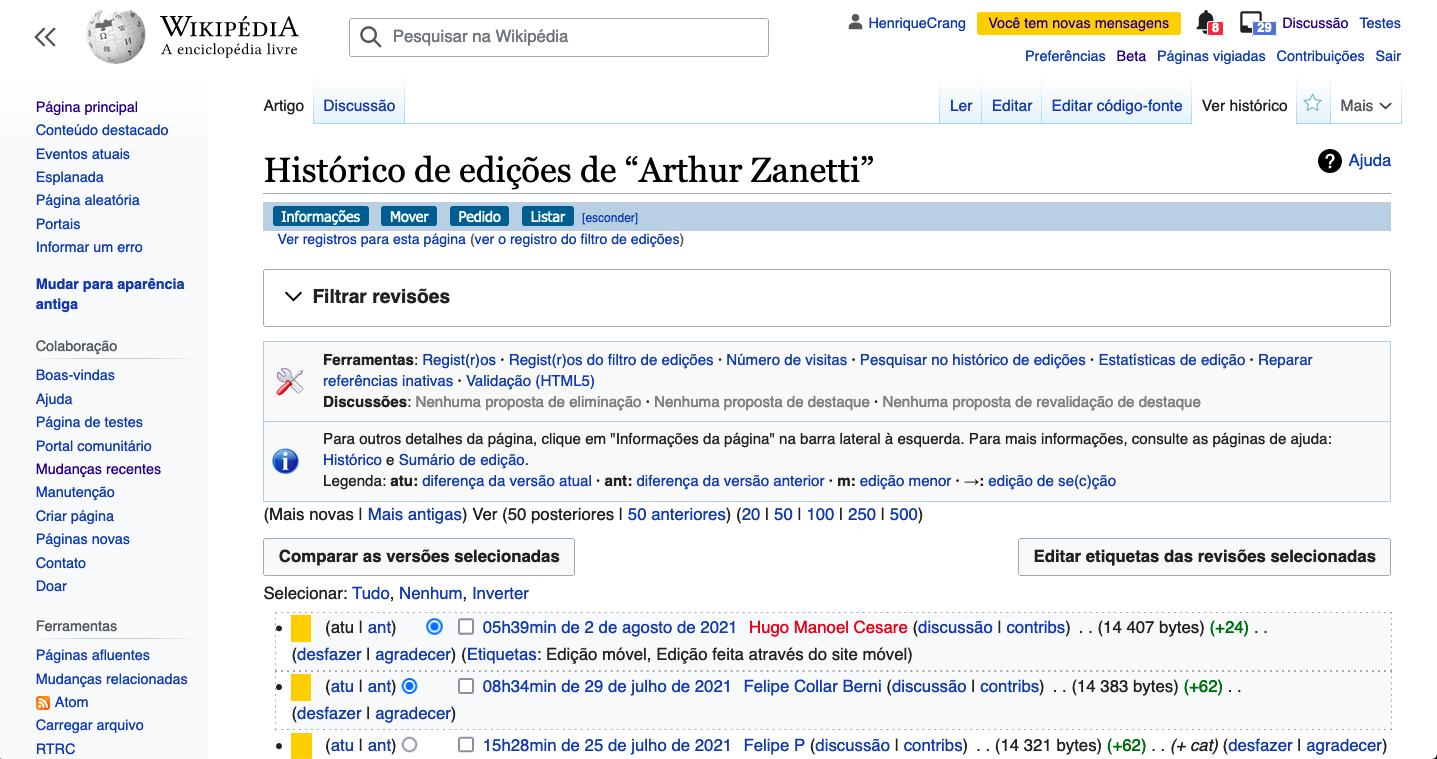
\includegraphics[width=1\textwidth]{Images/mediawiki_etiqueta.png}
    \caption{Exemplo do histórico de edições de uma página, com a edição mais recente recebendo duas etiquetas.}
    \label{fig:mediawiki_etiqueta}
\end{figure}

``Avisar'' já é uma ação que o filtro de edições toma que se faz imediatamente visível ao usuário, e altera sua experiência de edição no MediaWiki. Ao tentar salvar uma edição que algum dos filtros diga que deva ser ``avisada'', ao usuário será apresentada a seguinte mensagem:

\begin{figure}[H]
    \centering
    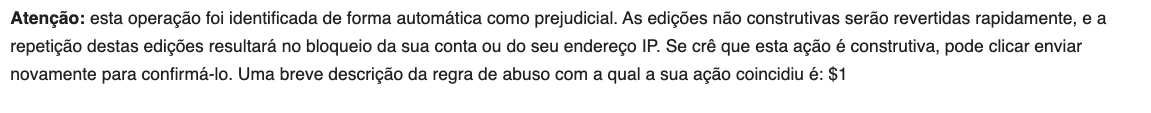
\includegraphics[width=1\textwidth]{Images/mediawiki_avisar.png}
    \caption{Mensagem padrão da função ``avisar'' do Filtro de edição. Para cada caso o ``\$1'' é substituído por uma mensagem do respectivo filtro despelotado. \citewiki{ptwiki_mediawiki_abusefilter_warning}}
    \label{fig:mediawiki_avisar}
\end{figure}

Após ser convidado a refletir se sua edição é ``construtiva'', o usuário tem então a opção de clicar novamente no botão de salvar e, nesta sua segunda tentativa, o MediaWiki deixará o conteúdo ser salvo.

Já a função de ``desautorizar'' é a mais drástica. Uma edição que se enquadre nos critérios de um filtro que preveja uma desautorização não poderá ser salva, e o MediaWiki apresentará ao usuário a seguinte mensagem:

\begin{figure}[H]
    \centering
    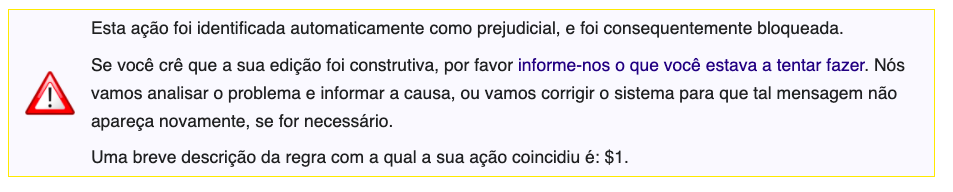
\includegraphics[width=1\textwidth]{Images/mediawiki_desautorizar.png}
    \caption{Mensagem padrão da função ``desautorizar'' do Filtro de edição. Para cada caso o ``\$1'' é substituído por uma mensagem do respectivo filtro despelotado.\citewiki{ptwiki_mediawiki_abusefilter_disallowed}}
    \label{fig:mediawiki_desautorizar}
\end{figure}

Desta forma, quando são utilizadas as ações ``avisar'' e ``desautorizar'' do filtro de edições, estão sendo tomadas decisões prévias sobre o que pode ser salvo. Estas decisões a \textit{priori}, tomadas e executadas de forma automática pelo MediaWiki, acontecem antes dos conteúdos chegarem aos espaços mais visíveis da Wikipédia, onde habitualmente acontecem discussões sobre a pertinência dos conteúdos.

%até aqui está explicando por alto como funcionam os filtros, agora começo a dar contexto pra eles. talvez quebrar seção?

Assim como acontece com a \textit{spam-blacklist}, os filtros também existem tanto em nível local nos projetos como a nível global para todas as wikis do movimento Wikimedia. Por padrão, os filtros globais são aplicados a todas as wiki consideradas de tamanho ``pequeno'' e ``médio'', e às wikis de grande porte que solicitarem sua inclusão. \footnote{``Global abuse filters were subsequently implemented and are set and operated from Meta-Wiki. These global filters apply to small[3] and medium[4] public WMF wikis, and those large wikis that opt-in.[5]. The stewards and meta administrators are able to set global abuse filters.[6]'' https://meta.wikimedia.org/wiki/AbuseFilter}

Desde de julho de 2016, a Wikipédia em português é umas das Wikipédias consideradas grandes que solicitaram sua ativação. A proposta de habilitar os filtros globais por lá foi feita pelo usuário He7d3r \footnote{He7d3r e o já citado Hélder são nomes diferentes utilizados ao longo do tempo pelo mesmo usuário.} no dia 02 de julho e, após receber o apoio de 13 editores fora aprovada sem nenhuma objeção. \citewiki{ptwiki_esplanada_proposta_filtros}. No dia 14/07 o pedido de alteração de configuração foi aberto no Phabricator \footnote{Sistema utilizado pelas comunidades técnicas para gerenciar tarefas. Falaremos mais sobre elas próxima seção.} e,  já em 18/07, dezesseis dias após a proposta ter sido feita e com a interação de 14 usuários, o Stashbot informava que a nova configuração, que dali para frente alteraria bastante a forma como usuários editam a enciclopédia, fora colocada em produção. (\cite{enable_global_abusefilters_ptwiki}).

Hoje, dentre as ditas grandes Wikipédias, além da versão em português, apenas as em francês e em cebuano também utilizam os filtros globais. \footnote{ Para encontrar está informação deve-se buscar no arquivo \textit{InitialiseSettings} da \textit{wikifarm} Wikimedia o seguinte comentário \textit{" // Enabled for all wikis that open, global and small/medium in size"}. O arquivo está disponível em  :https://noc.wikimedia.org/conf/InitialiseSettings.php.txt )}

%aqui parece haver uma mini quebra de seção tb. falei antes da instalacao, agora falo do estado da arte 

Atualmente existem 69 filtros globais ativos, sendo que a grande maioria trabalha buscando padrões de vandalismo \citewiki{enwiki_wikimedia_abuse_filter_management}. Na Wikipédia em português o mais ativo é o filtro global 206, que nos últimos 30 dias foi disparado 4611 vezes, correspondendo a edições que adicionavam links externos feitas por usuários com menos de duas edições. \citewiki{enwiki_editing_abuse_filter_206} Dentre os filtros globais que desautorizam edições, os mais ativos na enciclopédia lusófona são o 72, o 222 e o 240, com respectivamente 55, 28 e 24 edições desautorizadas nos últimos 30 dias \citewiki{ptwiki_acoes_filtros}.

Enquanto o filtro 222 pode ter seu funcionamento auditado por qualquer um, com seu código-fonte responsável por identificar a criação de páginas novas em branco por usuários novatos \citewiki{metawiki_editing_abuse_filter_222} visível para qualquer um que saiba navegar até sua página, os filtros 240 \citewiki{enwiki_editing_abuse_filter_240}e 72 tem seus códigos ocultados \citewiki{enwiki_editing_abuse_filter_72}, e deles podemos apenas ter acesso aos nomes: `\textit{Cannabis/CBD spam}' e `\textit{Global ``ntsamr''-pattern spambot filter}', mas sem podermos observar o código fonte dos mesmos.

\begin{figure}[H]
    \centering
    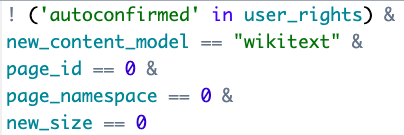
\includegraphics[width=1\textwidth]{Images/codigo_fonte_global_222.png}
    \caption{Código-fonte do filtro global 222. \citewiki{metawiki_editing_abuse_filter_222}}
    \label{fig:codigo_fonte_global_222}
\end{figure}

Tanto os filtros globais como os locais podem ser ``públicos'' ou ``privados''. Um filtro considerado ``público'' é o padrão, onde todas as regras e códigos executados por ele estão publicizados e abertos para receber críticas, comentários e melhorias de toda a comunidade. Já os filtros ``privados'' se valem da chamada ``segurança por obscuridade''. Costumam conter códigos para freiar spams que ``poderiam ser facilmente burlados se o atacante conhecesse a regra'', e então por isso tem seu código fonte aberto apenas para administradores.

De todos os 69 filtros globais atualmente ativos, 18 são ``públicos'' e 51 ``privados''. Quando ocorreu a aprovação da utilização dos filtros globais na Wikipédia em português, nenhum dos 13 editores que participaram do diálogo se preocuparam em ter algum tipo de acesso ao código fonte destes filtros globais fechados, que foram aprovados como confiáveis caixas pretas. \citewiki{enwiki_abuse_filter_management_100_pages}

\begin{figure}[H]
    \centering
    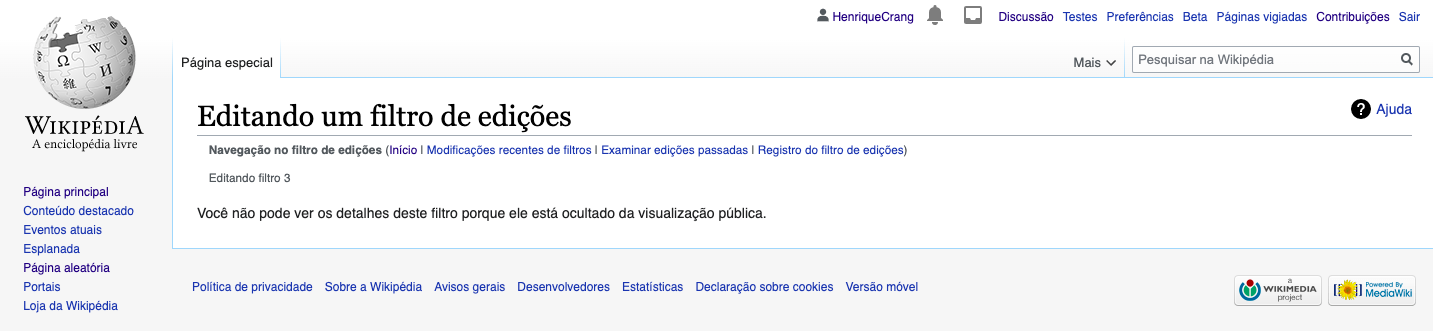
\includegraphics[width=1\textwidth]{Images/pagina_filtro_privado.png}
    \caption{Página especial de um filtro privado \citewiki{ptwiki_pagina_filtro_privado}.}
    \label{fig:pagina_filtro_privado}
\end{figure}

%dei aqui uma geral em filtros globais e seu impacto local. talvez possa trazer para cá umas coisas que já tenho rascunhadas sobre local/global

% agora vou entrar em mais detalhes da criação de filtros na ptwiki

Já dentre os filtros locais, criados pela própria comunidade da Wikipédia em português, os principais com a função de ``desautorizar'' são públicos. Os filtros 113, 18 e 70, com mais de 250 mil edições desautorizadas cada, podem ter seus códigos sobre \textit{"Página nova possivelmente sem referências"}, \textit{"Conteúdo e/ou resumo indevido"} e \textit{"Conteúdo e/ou resumo indevido relacionado ao corpo humano"} amplamente escrutinados pela comunidade. Já os três mais ativos filtros que ``avisam''; 3, 139 e 112, são privados, e por essa característica nossa pesquisa não pode ter acesso direto, através da página de filtros do MediaWiki, ao seu número de ações realizadas.

Porém, driblando de alguma forma a obscuridade de informações pelas páginas do MediaWiki, percebemos que ao ordenar os filtros por sua \textit{``contagem de correspondências''}, conseguimos ter uma ideia da escala da atividade dos filtros privados. Conforme pode ser visto na próxima figura, o filtro 03, sobre \textit{``Remoção considerável de conteúdo''} é o mais ativo na Wikipédia lusófona, com mais ações que o segundo colocado, que apresenta publicamente aproximadamente 267 mil ações.

\begin{figure}[H]
    \centering
    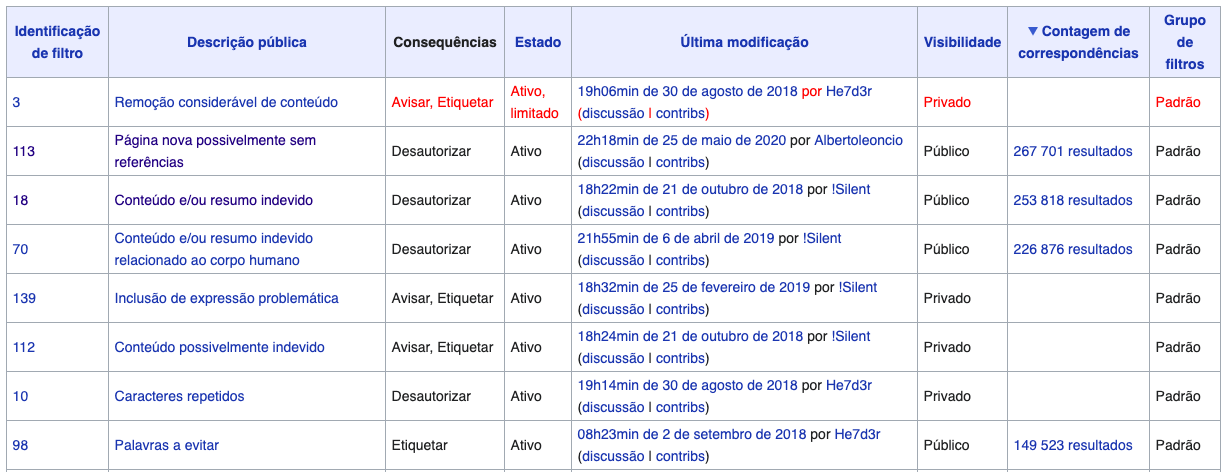
\includegraphics[width=1\textwidth]{Images/historico_filtros_wikipedia.png}
    \caption{Histórico dos filtros da Wikipédia em português ordenados por ``Contagem de correspondências'' \citewiki{ptwiki_administracao_filtros_abusos_100}}
    \label{fig:historico_filtros_wikipedia}
\end{figure}

Já os filtros 139, sobre \textit{``Inclusão de expressão problemática''} e 112 para \textit{``Conteúdo possivelmente indevido''}, com seus nomes um tanto quanto vagos e códigos ocultos, aparecem com um volume de ações menor que 226 mil, mas superior a 149.523. \citewiki{ptwiki_administracao_filtros_abusos_100}

Avançando com nossa pesquisa, resolvemos ir além das páginas da interface do MediaWiki e, consultando os bancos de dados públicos da Wikipédia em português, descobrimos que os quantitativos precisos de ações performadas por cada filtro privado está disponível sim para todos (todos que saibam SQL e conheçam a estrutura do banco de dados do MediaWiki). Lá, no acesso direto aos bancos de dados, então descobrimos que o filtro 139 foi disparado mais de 177 mil vezes, enquanto o 112 está quase empatado com 176 mil avisos feitos. Se esses dois filtros estão dentro do quantitativo previsto, e seus números precisos não agregam mais que uma curiosidade à nossa pesquisa, o mesmo não pode ser dito sobre o filtro 03. 

Sobre o filtro mais ativo da Wikipédia em português, através das páginas públicas, sabíamos apenas que possuía mais disparos que o segundo colocado, que apresenta aproximadamente 267 mil ações, mas não tínhamos ideia da grandeza de sua liderança. Ao consultar o banco de dados, pudemos encontrar incríveis 654.358 edições ``avisadas'' e ``etiquetadas'' pelo privado filtro de ``Remoção considerável de conteúdo'', representando 144\% mais ações que o filtro que aparece em segundo lugar.

\begin{figure}[H]
    \centering
    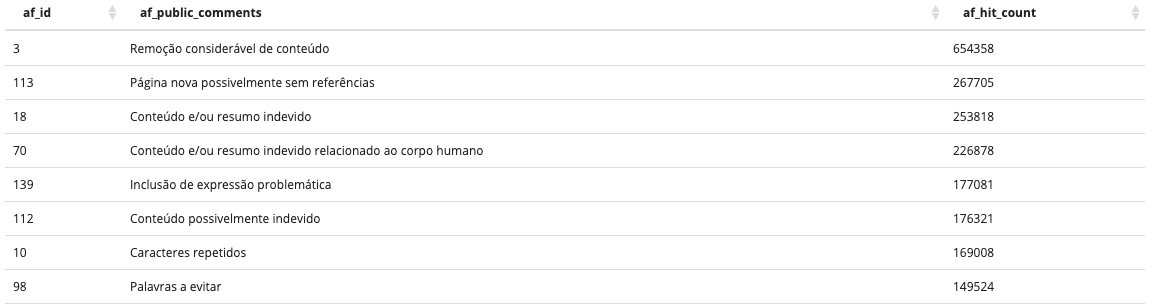
\includegraphics[width=1\textwidth]{Images/mediawiki_bancos_dados_publicos.png}
    \caption{Total de ações realizadas por cada filtro de edições da Wikipédia em português. Dados a princípio não disponíveis pela interface navegável do MediaWiki estão consolidados em bancos de dados públicos.
(\cite{quarry_most_hit_filters})}
    \label{fig:mediawiki_bancos_dados_publicos}
\end{figure}

Ao total, os filtros na Wikipédia em português já foram disparados 5.529.707 vezes (\cite{quarry_filters_count}). Destas, 2.444.513, ou 44\%, foram ações de ``avisos'', enquanto 2.149.290, ou 38,8\%, foram ações que desautorizaram uma edição. (\cite{quarry_warn_disallow_filter_actions}). Dentre todas essas ações que alteram o curso dos usuários, 1.581.419, ou 34,4\%, foram realizadas por filtros ``privados''. (\cite{quarry_warn_disallow_filter_actions_visibility})

Esse massivo volume de edições que tem seu curso esperado bloqueado pelo MediaWiki, através da configuração do filtro de edições, nos mostra que, enquanto alguns usuários devotam grande energia em discussões sobre eliminações e reversões de páginas avulsas, os poucos usuários que controlam os códigos fontes dos filtros atuam em uma escala muito maior. E esta ação em escala costuma passar despercebida pela comunidade, pois suas regras implementadas em códigos privados viram a lei que decide previamente não somente quais edições poderão ser salvas, mas também quais edições poderão ter sua validade debatidas, limitando quais que terão o privilégio de chegar aos espaços de escrutínio visíveis pela ampla comunidade.

\textbf{Como são criados os filtros de edições}

Sabendo de tamanha importância dos filtros de edições na Wikipédia buscamos então entender como eles são criados e editados. Assim como praticamente tudo que acontece no movimento Wikimedia, os filtros de edição são organizados através de páginas wiki. Porém, suas páginas seguem um padrão distinto do usual. Para cada filtro existe uma página ``Especial'', funcionalidade do MediaWiki que permite criar páginas com estruturas pré-prontas e com áreas pré-direcionadas de edição permitida, diferente das páginas padrão que podem ser inteiramente editadas.

\begin{figure}[H]
    \centering
    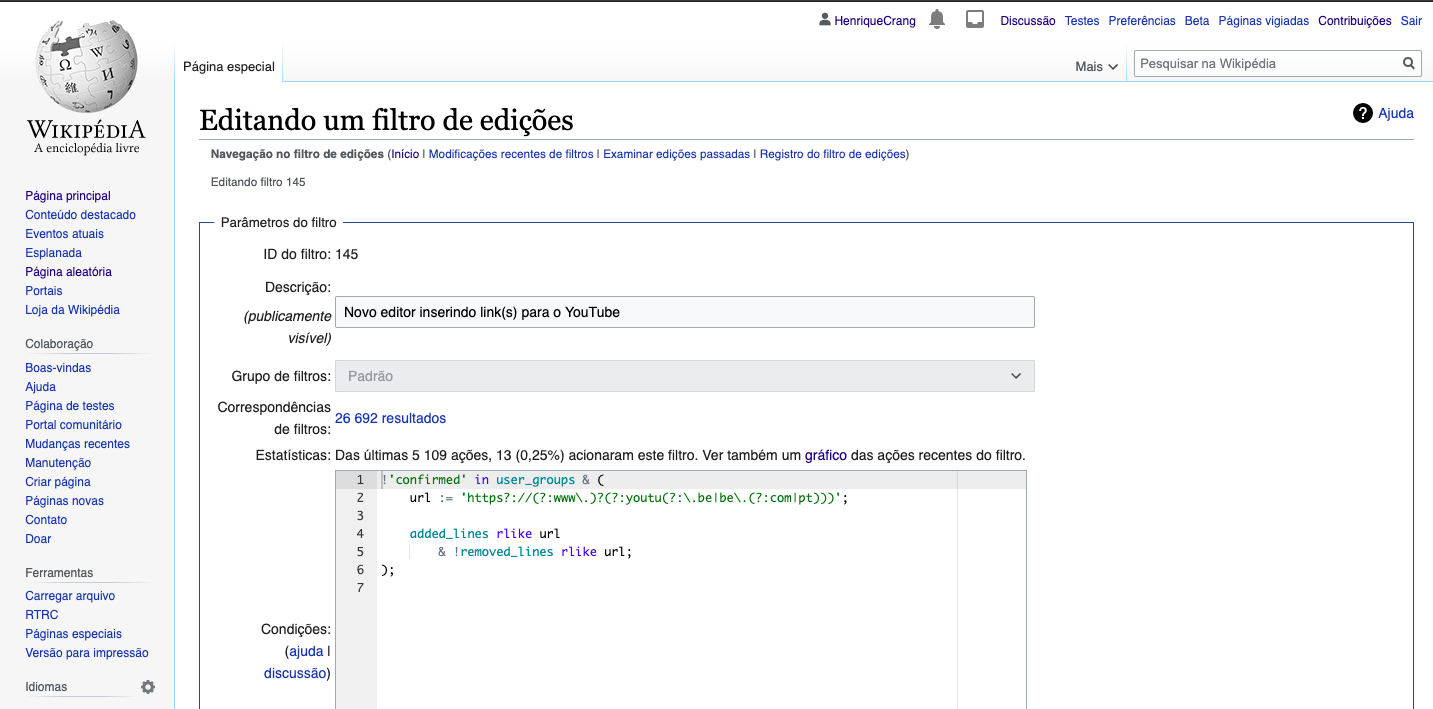
\includegraphics[width=1\textwidth]{Images/pagina_filtro_edicao.png}
    \caption{Exemplo de uma página especial relativa a um filtro de edição \citewiki{ptwiki_editar_filtros_edicao}.}
    \label{fig:pagina_filtro_edicao}
\end{figure}

Nestas páginas especiais, usuários administradores podem, para cada filtro, editar as expressões regulares, ativá-lo ou desativá-lo, configurar quais ações serão tomadas por ele, editar a mensagem que será exibida para o usuário que for identificado pelo filtro e deixar notas sobre seu trabalho realizado no filtro para auxiliar o trabalho de voluntários que venham a editá-lo no futuro.

\begin{figure}[H]
    \centering
    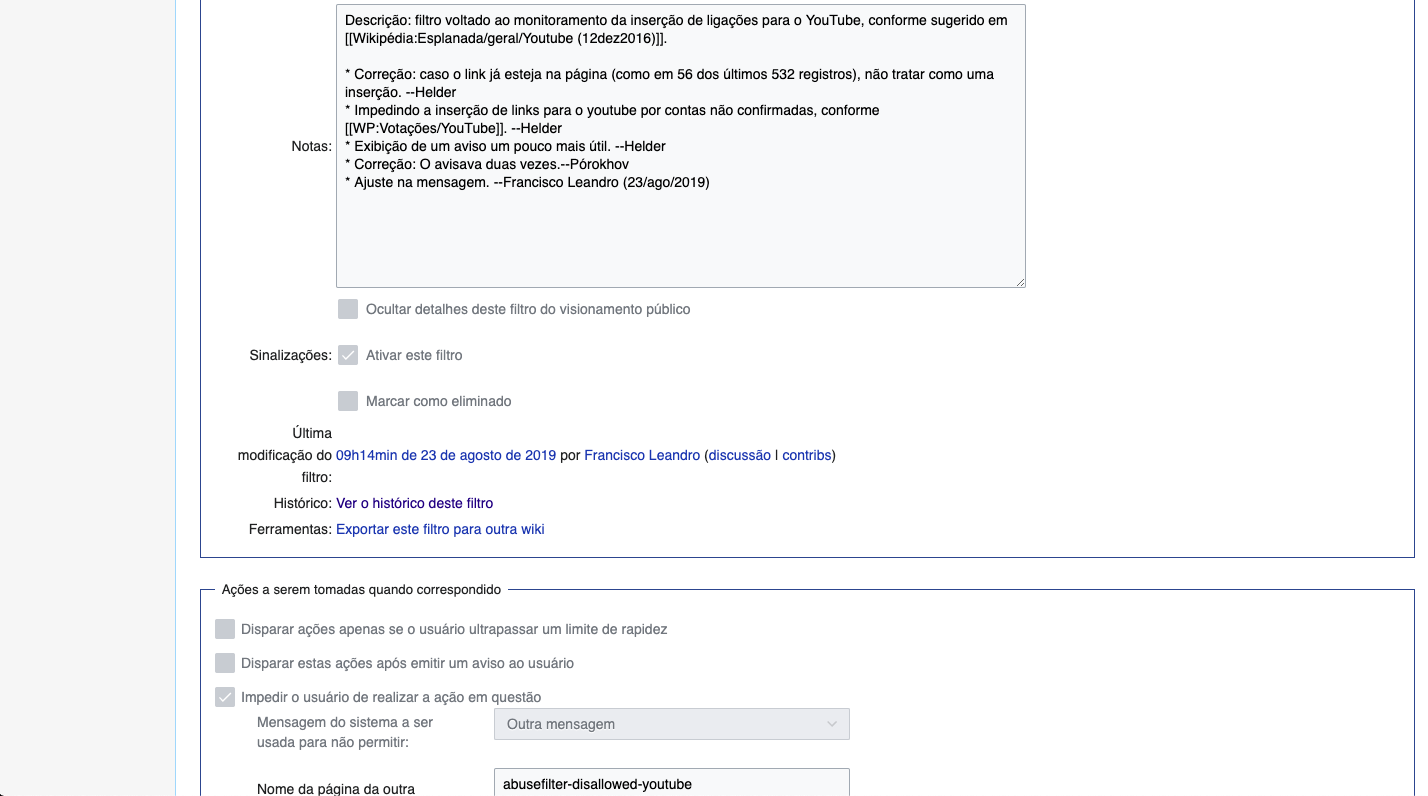
\includegraphics[width=1\textwidth]{Images/pagina_edicao_administadores.png}
    \caption{Continuação da página exibida na figura anterior, com mais opções de configurações dos filtros visíveis \citewiki{ptwiki_editar_filtros_1_edicao}.}
    \label{fig:pagina_edicao_administradores}
\end{figure}

Além das páginas especiais, existe uma página wiki ``comum'', que pode ser editada como as outras, que versa sobre os filtros de edição, explicando seu funcionamento. \footnote{Página disponível em https://pt.wikipedia.org/wiki/Wikipédia:Filtro\_de\_edições .} Assim como toda página wiki convencional, ela é acompanhada de uma página de discussão onde editores podem abrir tópicos para debater seu conteúdo.

Porém, esta página aparenta não contar com a atenção dos wikipedistas. Desde 2019 foram abertos 20 novos tópicos de discussão nela por usuários novatos mas, decorridos 8 meses do ano de 2020, apenas um havia recebido resposta de um editor experiente, com os demais 19 tópicos seguindo visíveis e ignorados. \citewiki{ptwiki_filtro_de_edicoes}

Até o final de 2019 existia uma outra página wiki, chamada ``Filtro de Edições/Solicitações'', que concentrava pedidos para alterações nos filtros. Nela podemos ainda encontrar assustadores 125 novos tópicos sobre o funcionamento dos filtros de edições que foram criados e não obtiveram nenhuma resposta. \citewiki{ptwiki_filtros_edicao_solicitacoes}

Durante um certo período de tempo, esta página recebia um volume de acessos maior de novatos, pois o aviso de ``desautorizar'' apresenta um link para ela com a seguinte mensagem \textit{``Se você crê que a sua edição foi construtiva, por favor informe-nos o que você estava a tentar fazer. Nós vamos analisar o problema e informar a causa, ou vamos corrigir o sistema para que tal mensagem não apareça novamente, se for necessário.''} \citewiki{ptwiki_mediawiki_abusefilter_disallowed}. Porém, desde o dia 1 de dezembro de 2019, quando foi aprovada uma proposta de fusão de diversas páginas de contato da Wikipédia em português \citewiki{ptwiki_esplanada_geral_duvidas-fale}, a mensagem de ``desautorizar'' dos filtros passou a linkar os usuários para a página ``Wikipédia:Tire Suas dúvidas''\citewiki{ptwiki_ajuda_duvidas}. Por ser esta uma página mais genérica onde são tratados diversos assuntos, não nos foi possível observar o volume de mensagens relativos a filtros que chegam até ela, mas cabe destacar que este novo destino é monitorado por mais wikipedistas, e são raros os novos tópicos abertos por lá que ficam sem resposta.

% aqui tem uma pequena mudança, vinhamos falando de onde os novatos são encaminhados, agora seguimos o rastro "mais pra dentro", buscando debates avançados

Seguimos buscando rastros de debates sobre os filtros, e adentramos o ``Café dos administradores'', uma página wiki que pode ser lida por todos mas somente pode ser editada por usuários com permissão de administrador. Voltando o histórico da página até o início de 2018, encontramos apenas uma menção ao filtro de edições, onde um administrador solicita ajuda de alguém \textit{``familiarizado com o assunto''} para implementar em filtro um bloqueio parcial a um usuário que fora decidido em uma votação. Em menos de 12 horas, o pedido foi respondido como um direto \textit{``feito''}, e nunca mais o filtro de edições fora mencionado no café dos administradores. \citewiki{ptwiki_diferenca_edicao_cafe-administradores}

% outra mudança no texto. indo atrás de depoimentos

Em meio a tão poucos debate e discussões, aceitamos então que seguir o rastro digital da criação dos filtros não estava apresentando muitos resultados para nossa pesquisa. Decidimos assim partir para o campo e conversamos com administradores da Wikipédia em português mais engajados na tarefa de criar, manter e atualizar filtros.

OTAVIO1981, ou simplesmente Otávio, é um usuário ativo da Wikipédia desde 2007. Com mais de 36 mil edições\citewiki{ptwiki_edicoes_grupos_otavio1981}, em março de 2015, ele que já havia sido administrador entre 2013\citewiki{ptwiki_administradores_pedido_otavio1981/1} e 2014\citewiki{enwiki_wikimedia_steward_resquest_permissions}, se propõe à assumir a posição novamente, dizendo explicitamente em seu pedido de aprovação que \textit{``firmo o compromisso de orientar e seguir com a atualização dos filtros de edição, etiquetas, e atualizações no mediawiki''} \citewiki{ptwiki_administradores_pedido_otavio1981}

Otávio, que não trabalha na área de computação, resolveu \textit{``estudar e aprender como fazer  expressões regulares para atuar com os filtros.''}\footnote{Até que seja indicado o contrário, todas as citações que seguem são retiradas da entrevista realizada com OTAVIO1981}, e se propôs a ser um voluntário que atua ativamente na melhoria desta ferramenta e na orientação a usuários que interajam com ela. Em sua candidatura a administrador em 2013, Otávio afirmou que desejava ter acesso administrativo pois \textit{``entendo que o acesso é prioritariamente para atuar na área de filtros que não possui instalado aqui outro estatuto que permita acesso as ferramentas necessárias''}.

Em outras palavras, como apenas administradores podem acessar as ferramentas completas dos filtros de edição, ele precisava ser um administrador da Wikipédia em português para seguir com suas contribuições nesta area\citewiki{ptwiki_administradores_pedido_otavio1981/1}. Novamente, em seu questionário de renomeação em 2015, o editor foi enfático ao afirmar que \textit{``O filtro de edições possui alguns recursos que estão disponíveis somente para administradores, assim como filtros que são privados, portanto não é possível orientar a atualização para terceiros sem acesso a estes recursos''}. Assim como em 2013, o novo pedido de Otávio para se tornar administrador é aprovado sem nenhum voto contrário.

% aqui teve uma apresentacao do Otavio virando admin para poder mexer nos filtros, para baixo entra já numa explicao da criacao dos filtros, que estavamos procurando

Otávio nos conta que houveram três grandes \textit{``ondas de atividade''} na construção e melhoria de filtros na Wikipédia em português, em momentos que alguns voluntários se dedicaram mais intensamente a melhorá-los. Houve uma primeira onda inicial quando os filtros foram implementados entre 2009 e 2010, uma segunda onda em 2013, da qual ele participou ativamente, e depois uma terceira onda em 2017. 

\begin{figure}[H]
    \centering
    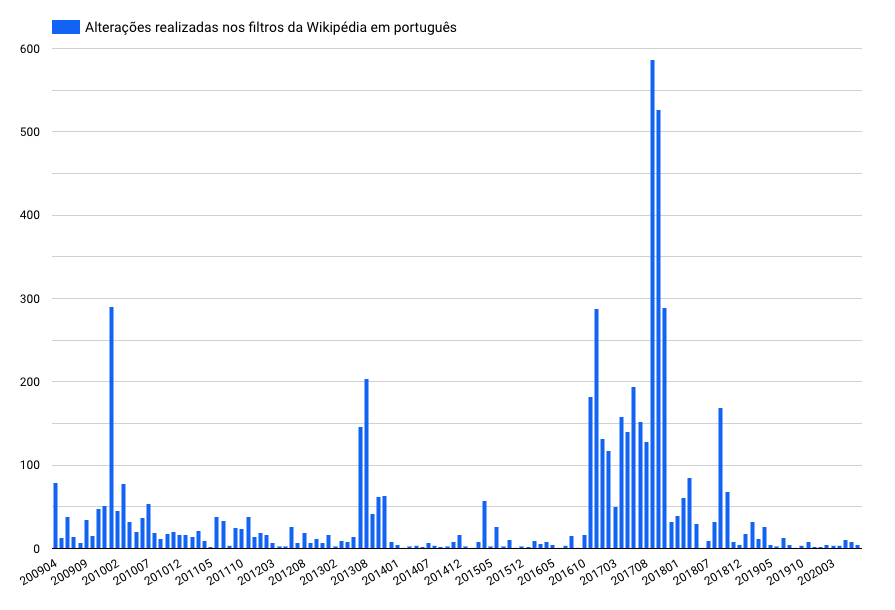
\includegraphics[width=1\textwidth]{Images/grafico_alteracoes_filtros.png}
    \caption{Volume de alterações nos filtros da Wikipédia em português por mês, onde poder ser visualmente identificadas as três ondas de atividade. (fonte: https://datastudio.google.com/u/0/reporting/6b38f843-1507-4364-85e9-bdef43296881/page/TRabB ).}
    \label{fig:grafico_alteracoes_filtros}
\end{figure}

Otávio esteve muito ativo na onda de interesse pelos filtros em 2013, que aconteceu devido a polêmica retirada do modo emergencial do CAPTCHA \footnote{Esta polêmica será detalhada mais a frente no texto.}. Esta ação fez o número de edições na Wikipédia em português subir e levou a comunidade a buscar novas formas de automatizar o combate a edições ruins.

O usuário explica que nesta segunda onda, \textit{``apesar de não terem conseguido chegar em uma \textbf{formalidade científica} para validar se um filtro estava dando resultado''} (grifo nosso), criaram critérios para testar os filtros e decidir se eles seriam \textit{``promovidos''}.

Neste processo foi realizada uma força tarefa para avaliar cada disparo dos filtros, apontando se fora um ``verdadeiro positivo'' ou um ``falso positivo''. Assim, para cada filtro foi criada uma página wiki onde o resultado da avaliação de todas as suas ações deveria ser publicado \footnote{Um exemplo de página de avaliação dos filtros pode ser encontrado em: https://pt.wikipedia.org/wiki/Wikipédia:Filtro\_de\_edições/An\%C3\%A1lise/Filtro\_70}. Visando facilitar não só o trabalho de avaliação dos disparos dos filtros como também a futura agregação e comparação dos dados gerados, o usuário He7d3r criou um script \footnote{Disponível em meta.wikimedia.org/w/index.php?title=User:He7d3r/Tools/AbuseLogStatus.js} para automatizar a geração destas avaliações de forma rápida e padronizada.

Foram realizadas aproximadamente 7 mil avaliações das ações dos filtros e, apesar de toda a comunidade ter sido convidada a colaborar, mais de 92\% das ações foram realizadas por apenas 3 usuários (OTAVIO1981, Rjclaudio e He7d3r), sendo OTAVIO1981 sozinho responsável por mais da metade delas. Vale mencionar que sempre que um usuário anotava que uma edição fora um ``falso positivo'', ele era convidado a escrever um comentário sobre sua avaliação, e estes comentários posteriormente seriam utilizados para buscar realizar melhorias nos filtros.

\begin{figure}[H]
    \centering
    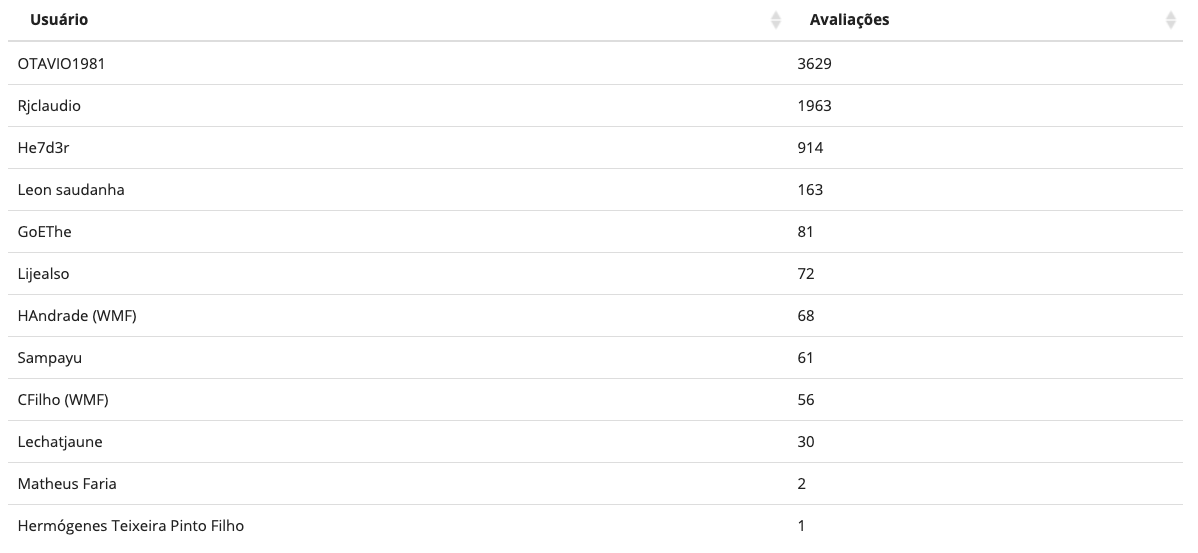
\includegraphics[width=1\textwidth]{Images/pagina_analise_filtros.png}
    \caption{Edições feitas nas páginas de Análise dos Filtros (\cite{quarry_users_evaluating_filters}).}
    \label{fig:pagina_analise_filtros}
\end{figure}

Não por acaso, estes mesmo três usuários mais ativos na avaliação dos filtros foram também os mais ativos na edição dos mesmos durante a chamada segunda onda. Entre julho e novembro de 2013, Rjclaudio realizou 286 alterações nos filtros, seguido por He7d3r com 139 e Otávio com 51.

Durante os esforços da segunda onda, os usuários mais engajados na melhoria dos filtros debatiam em um espaço público\citewiki{ptwiki_discussao_filtro_edicao_analise} os resultados encontrados e coordenavam ali as alterações que seriam feitas. Os índices de acertos e erros de cada filtro avaliado passaram a ser consolidados em uma página, disponível até hoje no endereço https://pt.wikipedia.org/wiki/Wikipédia:Filtro\_de\_edições/Análise. 

Nestas páginas de análise, foi possível observar que vários filtros apresentavam um volume consideravelmente alto de erros, de onde podemos destacar os já citados filtros 113 e 70, que são os mais ativos na Wikipédia em português na ação de ``desautorizar'' uma edição. Para nossa surpresa, observamos que das 112 ações do filtro 113 avaliadas pela força tarefa, 31,3\% foram consideradas falsos positivos e, com um espaço amostral maior, com 570 edições avaliadas, o filtro 70 aparenta ter sido disparado indevidamente 22,8\% das vezes.

Estes grandiosos números aparentavam anunciar um cenário trágico, mas ao analisarmos o histórico de edições destes filtros podemos entender melhor o que estava acontecendo. Seguindo o que Otávio chama de \textbf{\textit{``uma busca por formalidade científica''}}, os filtros estavam sendo criados somente com ações de etiquetar, para serem testados na vida real, avaliados, melhorados, e apenas passariam a performar ações mais drásticas quando apresentassem resultados considerados satisfatórios.

Ao olharmos o caso de filtro 113, por exemplo, identificamos 13 edições nele durante a segunda onda\citewiki{ptwiki_filtro_abuso_historico113} antes que fosse chamado a realizar qualquer ação que interferisse no curso dos usuários. Após diversas revisões iniciais, o filtro passa para fases de testes, onde são intercaladas as ações de “etiquetar”, “avisar” e “desautorizar”, se estabilizando ao final da onda, em novembro de 2013, como um filtro que “apenas” etiqueta.

Em abril de 2014 ele viria a ser novamente alterado para se tornar um filtro que também “avisa”, voltando a ser um “desautorizador” apenas em março de 2018, após uma proposta aprovada na Esplanada \citewiki{ptwiki_esplanada_geral_verificabilidade_artigos}.

A proposta acima, após uma breve discussão que contou com o apoio de quatro usuários e nenhuma objção, foi implementada pelo usuário “Silent!”. Ele que, desde sua nomeação para administrador em 2016, se tornou o usuário mais ativo da história da Wikipédia em português nos filtros de edição. Silent, um programador de carreira, nos conta \footnote{Até que seja indicado o contrário, todas as citações que seguem são retiradas da entrevista realizada com ``Silent!''.} que após se tornar administrador da Wikipédia em português percebeu que existia uma defasagem nos filtros, que não eram atualizados há um tempo, e passou a se dedicar intensamente a esta tarefa.

Sua determinação cria então o que chamamos de “terceira onda” de filtros na Wikipédia em português, que começa em novembro de 2016 e vai até novembro de 2017. Durante ela, Silent é responsável por 2675 edições nos filtros, respondendo assim por mais de 90\% das ações ali realizadas no período.

O usuário nos conta que \textit{“a alta defasagem dos filtros me levou a criar e adaptar muita coisa que já existia para se atualizar aos problemas de vandalismo da época. Para se ter uma noção, os filtros não barravam diversos xingamentos extremamente nocivos em português de Portugal, como “pila” e “cona”, que são palavrão que remetem ao órgão sexual masculino e feminino, respectivamente; ou seja, eles retratavam uma visão muito mais brasileira da coisa, deixando de lado ofensas em português europeu”}.

Em seu processo de melhoria dos filtros ele lamenta que a ferramenta não permita exibir um \textit{feedback} maior para os usuários que estão adicionando conteúdo considerado problemático: \textit{“não é possível exibir, naquele aviso que aparece após uma edição ser bloqueada por um filtro, qual é expressão que gerou o bloqueio”}, e também nos conta que a página para onde outrora os usuários eram encaminhados cumpria um papel importante no trabalho de adequação dos filtros para diminuir os falsos-positivos. \textit{“Foi por ali [Página Wikipédia:Filtro de edições/Solicitações] que eu fiquei sabendo de vários falsos-positivos gerados em modificações feitas por mim nos filtros.}”

Perguntado sobre a necessidade de encaminhar propostas de alterações nos filtros para a comunidade, o usuário nos explica que \textit{“na realidade não há um local específico para o debate de alterações nos filtros e nem há uma necessidade de que cada novo filtro seja implantado via consenso. Todas àquelas alterações feitas por mim, principalmente no fim de 2016 e por todo ano de 2017, foram feitas de forma unilateral”}, complementando que seu processo de controle de qualidade dos mesmos é feito de forma artesanal: \textit{“da minha parte, são todos testados individualmente e de forma manual, disparo por disparo a fim de identificar problemas ou oportunidades de melhoria. Não há uma página específica, mas há uma ferramenta que contabiliza o índice de disparos”}.

%aqui dou uma desviada para falar do ptwikis

A citada ferramenta é parte do projeto PTWIKIS, e fora criada pela comunidade lusófona, com especial liderança do usuário danilo.mac, durante a segunda onda de filtros. O “ptwikis” é um projeto de criação de ferramentas de visualização de dados que exibe gráficos rápidos para uma série de informações sobre as Wikipédias, \textit{“criado para concentrar em um único projeto ferramentas que sejam de interesse dos projetos lusófonos e para incentivar a cooperação entre usuários para o desenvolvimento dessas ferramentas”}. \citewiki{ptwiki_ptwikis}

Apesar de inicialmente criada pela e para a Wikipédia em português, hoje a ferramenta apresenta opções para seus dados serem gerados sobre qualquer wiki dentro do movimento Wikimedia, e também é utilizada por editores de outros projetos e idiomas. Em sua seção dedicada ao monitoramento de filtros, a ferramenta exibe duas telas, uma com todos os filtros e suas ações totalizadas nos últimos 30 dias \citewiki{ptwiki_acoes_filtros} e  outra com uma linha do tempo, exibindo as ações dos filtros selecionados totalizadas por dia \citewiki{ptwiki_acoes_filtros_exemplo3_7}.

O projeto ptwikis fora criado não coincidentemente em julho de 2013, exatamente quando se iniciava a segunda onda de melhoria dos filtros. A remoção do modo emergencial do CAPTCHA acontecida no início daquele ano aparenta ter gerado um grande efeito catalisador na comunidade da Wikipédia em português, que passou a buscar conhecer melhor suas dinâmicas e ferramentas. Para compreendermos o que aconteceu no referido evento e entendermos o tamanho de sua influência na comunidade, exploraremos o funcionamento da ferramenta de CAPTCHA na próxima seção.

\subsection{CAPTCHA}

CAPTCHA, sigla em inglês para \textit{``Completely Automated Public Turing test to tell Computers and Humans Apart''} \footnote{Em tradução livre: \textit{“teste de Turing público completamente automatizado para diferenciação entre computadores e humanos”.}}, é uma ferramenta muito comum na internet para tentar evitar ações automatizadas realizadas por \textit{``robôs mal intencionados''}. \citewiki{ptwiki_captcha_definicao}

Na Wikipédia, o captcha se materializa em forma de palavras em inglês onduladas e picotadas, em um padrão que seus desenvolvedores esperam ser muito complicado para robôs entenderem, mas simples para humanos. \citewiki{ptwiki_captcha_definicao}

\begin{figure}[H]
    \centering
    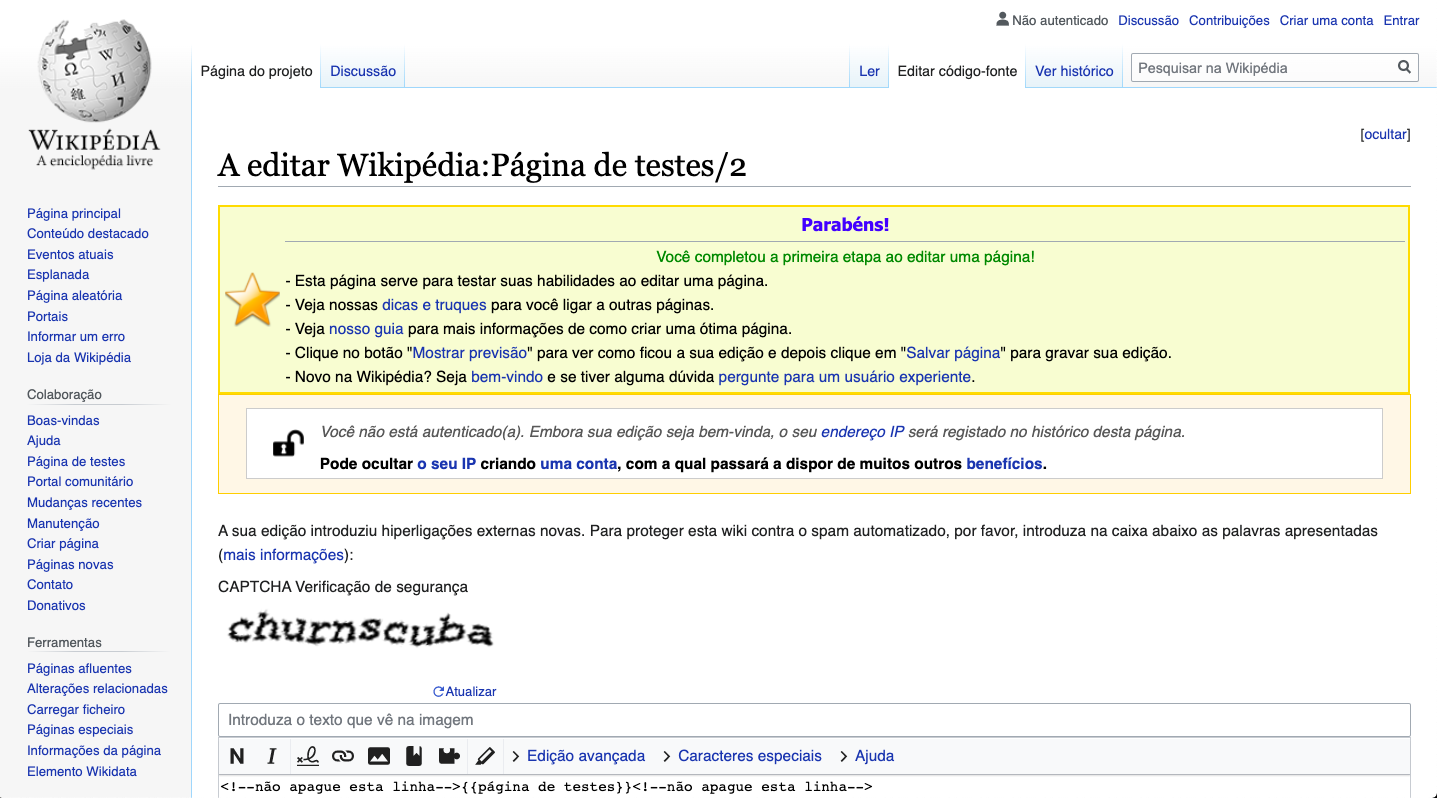
\includegraphics[width=1\textwidth]{Images/mediawiki_solicita_captcha.png}
    \caption{MediaWiki solicitando que um usuário anônimo resolva um captcha para salvar sua edição. Detalhe para a caixa de \textit{“parabéns por sua primeira edição feita”} erroneamente sendo exibida em destaque, mesmo com a edição não tendo ainda de fato sido salva.}
    \label{fig:mediawiki_solicita_captcha}
\end{figure}

O teste é implementado pela \textit{ConfirmEdit}, uma extensão feita para o MediaWiki que, desde a versão 1.18 do software, já é distribuída com ele por padrão. Segundo o \textit{Wikiapiary}, hoje essa ferramenta de CAPTCHA para MediaWiki é utilizada por aproximadamente 10 mil wikis diferentes pelo mundo\citep{extension_confirm_edit}.

Tanto a página oficial da extensão\citewiki{enwiki_extension_confirm_edit} como a página na Wikipédia em português sobre a ferramenta \citewiki{ptwiki_captcha_definicao} afirmam que ela é utilizada para coibir spambots, \textit{“que, através de contas anônimas, provocam vandalismo em diversos artigos em um curto espaço de tempo”}. Visando alcançar este objetivo, atualmente a configuração padrão do CAPTCHA nas Wikipédias dita que ele deve aparecer sempre que um usuário anônimo ou não confirmado (também chamado de novato) fizer uma edição adicionando um link externo.

A expectativa anunciada pelos wikipedistas é que humanos consigam facilmente resolver o teste, e apenas os scripts maliciosos sejam barrados pela ferramenta. Porém, a realidade não se mostra tão óbvia. Na própria página sobre a ferramenta existem três notas de rodapé apontando para transbordamentos da atuação do captcha: [1] o fato das palavras serem em inglês aumenta a dificuldade de compreensão de não falantes deste idioma, [2] usuários cegos não tem chances de resolver este captcha, que é totalmente dependente da visão e [3] quando ativado o modo emergencial, todas as edições feitas por anônimos e novatos, adicionando ou não links externos, precisam resolver o captcha. \citewiki{ptwiki_captcha_definicao}

Das três controvérsias listadas pelos wikipedistas sobre o captcha decidimos em nossa pesquisa seguir a terceira, pois fora exatamente a desativação deste modo emergencial em 2013 que desencadeara a segunda onda de filtros trabalhada na seção anterior.

% aqui acaba uma introdução ao captcha e começa a controvérsia

No dia 8 de abril de 2013, o usuário Helder.wiki cria um tópico na página ``Esplanada/anúncios'', o fórum central de notícias internas da Wikipédia em português, intitulado \textit{``Remoção do modo emergencial do CAPTCHA''}, e seu conteúdo tem apenas o texto \textit{``Ver gerrit:58081''}, com um link para um ticket no sistema de revisão de scripts dos servidores do Movimento Wikimedia, onde o código da anunciada alteração havia sido aprovado para ser executado nos servidores da Wikipédia em português. Este acontecimento desperta revolta em vários membros da comunidade lusófona e controvérsias tanto sobre a governança da comunidade como sobre o controle de qualidade dos verbetes se acaloram. \citewiki{ptwiki_esplanada_geral_remocao_modo_captcha}

É interessante notar que o uso do modo emergencial do CAPTCHA havia sido deslocado pela comunidade lusófona. Enquanto originalmente pensada e documentada para ser utilizada contra robôs maliciosos, a ferramenta passou a ser vista pela Wikipédia em português como uma ajudante na diminuição do volume de edições potencialmente ruins que precisariam ser revisadas por humanos.

A discussão na Esplanada então segue com mensagens em português, inglês e italiano, pois fora um usuário nativo deste idioma que encaminhara a desativação do modo emergencial. Ação essa tomada após o mesmo ter notado o modo emergencial \textit{“esquecido ativo”}, depois de ter sido ligado durante um ataque de robôs spammers no longíquo janeiro de 2008\citewiki{ptwiki_esplanada_arquivo_2008janeiro}.

Sentindo ter sua autonomia ferida, vários membros da comunidade lusófona acusam a \textit{“comunidade técnica de administradores de servidores”} de ingerência, e partem para travar o debate em outros espaços do movimento Wikimedia. Assim, locais como o Bugzilla (hoje rebatizado Phabricator) \citep{remove_ptwiki_ptwikinews_captcha_mode} e até mesmo o Gerrit \citewiki{remove_ptwiki_ptwikinews_captcha_mode_gerrit}, sempre vistos como \textit{``espaços técnicos''}, onde são discutidas apenas formas de fazer o software funcionar, e não as decisões das comunidades, acabam se tornando palco de discussões e acusações sobre governança dos projetos, definições de consensos e esforços de combate ao vandalismo.  

Aproximadamente 24 horas após o anúncio feito por Helder.wiki na Esplanada, a mudança estava efetivada e o modo emergencial do captcha removido da Wikipédia em português. O usuário Rjclaudio então propõe que pesquisas sejam feitas para medir mudanças de comportamento e testar na prática se os cenários apocalípticos decorrentes desta mudança de configura/cão, alardeados por alguns usuários no acalorado debate, se tornariam realidade. Assim, vemos a emergência de centrais de cálculo da comunidade e esforços para criação de métricas que traduzam as “percepções subjetivas” sentidas pelos usuários em “números objetivos”. Observamos então a tentativa de estabilização de traduções. Dois grupos diferentes buscam fazer inferências e convencer o movimento que a sua interpretação seria a forma certa de ler os dados, com os mesmos números servindo de base tanto para teses de que a desativação do modo emergencial do CAPTCHA havia sido benéfica, tanto como para a interpretação de que essa ação estaria matando o projeto. Temos então colocada uma disputa entre duas realidades diferentes, que por serem contraditórias e disputarem o mesmo espaço de poder, precisam provar como falsa a tese adversária para poder sair vitoriosa da peleja e então nortear as ações a serem tomadas em seguida.

É interessante notar a riqueza de desdobramentos que uma pane pode causar. Diversas iniciativas são tomadas para criar novas composições estáveis para a manutenção e continuidade do projeto, e uma vez aberta a caixa-preta das edições represadas pelo modo Emergencial do Captcha não será mais satisfatório e suficiente simplesmente o ativar novamente para encerrar a controvérsia. Agora existe uma boa parcela de usuários genuinamente preocupados e engajados em entender quais edições que outrora estavam represadas por essa configuração agora estão sendo feitas, e qual o perfil de usuários que as estão fazendo. 

Com isso, as barreiras automatizadas para edições implementadas no MediaWiki passam a ser vistas como um ponto de passagem obrigatório no debate sobre o crescimento da comunidade e a recepção de novos usuários, e algumas destas barreiras implementadas em software passarão então a receber atenção e ser dissecadas por alguns usuários mais dedicados ao assunto.


Em meio diversas visões de mundo, disputas e acusações, a comunidade lusófona parece se aproximar de um consenso sobre a tão polêmica configuração, que arriscamos resumir em ``O modo emergencial do CAPTCHA ajuda no controle de qualidade ao diminuir o volume de edições, mas queremos controlar a qualidade de outra forma que não tornando a vida de quem quer editar mais difícil'' \footnote{Para mais detalhes sobre esta controvérsia ver https://pt.wikipedia.org/wiki/Wikipédia\_Discuss\%C3\%A3o:Captcha\#Apanhado\_de\_discuss\%C3\%B5es\_sobre\_o\_CAPTCHA\_para\_registo}. 

Em um movimento de construção de novas formas de combate às edições consideradas ruins, que não passasse simplesmente por dificultar a vida dos usuários novatos, a Wikipédia em português assiste então ao renascimento do ``Projeto Antivandalismo'', que apesar de existir desde 2008, estava praticamente inativo por anos e passa a receber diversas contribuições ao longo do ano de 2013.

\begin{table}
\centering
\begin{tabular}{c|c}\hline
 \textbf{Ano} & \textbf{Edições}\\ \hline
    2017 & 2\\\hline
    2016 & 10\\\hline
    2015 & 6\\\hline
    2014 & 24\\\hline
    2013 & 364\\\hline
    2012 & 2\\\hline
    2011 & 0\\\hline
    2010 & 7\\\hline
    2009 & 13\\\hline
    2008 & 27\\\hline
\end{tabular}
\caption{Total de edições por ano na página Wikipédia Discussão:Projetos/AntiVandalismo.\citep{quarry_edits_page_year}}
\label{tab_edicao_wiki_antivandalismo}
\end{table}

Em paralelo, enquanto busca criar alternativas futuras de controle de qualidade,  a comunidade lusófona solicita a intervenção da WMF na ``crise diplomática'' instaurada dentro do movimento Wikimedia, pedindo que sua autonomia seja respeitada pela ``comunidade do MediaWiki'', e que o modo emergencial do CAPTCHA seja reativado. O pedido deixa claro não haver um ``argumento técnico'' para comprovar ataques de robôs, e deixa explícito seu intuito de diminuir o volume de edições feitas por novatos. A fundação então responde que esta não é a função da ferramenta, mas que, por ela ter sido esquecida ativada por tanto tempo, iria então permitir temporariamente sua reativação até o final de 2013, reforçando que o combate a edições ruins deveria a partir de então ser feito por outros meios, como os que estavam sendo discutidos no \textit{``Projeto Antivandalismo''}.  \citewiki{ptwiki_discussao_captcha}

Desta forma, diversos usuários se engajam em projetos tanto para freiar automaticamente edições não desejadas (criando a segunda onda de atualização dos filtros), como para desenvolver ferramentas de análise e monitoramento de metadados de comportamento na comunidade (criando o já citado projeto “ptwikis”), como também para melhorar a recepção de novatos bem intencionados (iniciativas que serão citadas no próximo capítulo). Assim, com a comunidade engajada em diversas novas formas de combate ao vandalismo e a melhoria na recepção de novatos, ao se iniciar o ano de 2014, o modo emergencial do CAPTCHA é finalmente desativado sem maiores controvérsias.

%aqui acaba a treta de 2013 e começo a falar de como essa ferramenta é monitorada hoje

Passados seis anos da contenda e da reestabilização do CAPTCHA como uma ferramenta que deve apenas combater \textit{“robôs spammers maliciosos”} e não usuários inexperientes, buscamos saber como a comunidade da Wikipédia em português monitora o funcionamento da ferramenta.

Começamos nossa busca pelas páginas dentro da Wikipédia sobre a ferramenta do captcha, mas encontramos apenas textos informativos. A página de discussão da ferramenta, bastante acalorada no passado, não recebe nenhuma contribuição desde julho de 2013.

Não encontrando indícios de monitoramento da ferramenta pelas páginas wiki, resolvemos buscar informações com os usuários mais engajados nos filtros com quem conversamos. Apesar das ferramentas serem próximas e terem funcionalidades parecidas, tanto Otávio como Silent, que são engajados no acompanhamento dos filtros, não souberam responder onde e/ou se existe um log com as edições desautorizadas pelo CAPTCHA, e desconhecem a possibilidade de se realizar uma auditoria em seu funcionamento. 

Buscamos então o maior fórum público da Wikipédia em português: a Esplanada. A Esplanada é um conjunto de páginas dentro da Wikipédia onde usuários podem fazer comentários, propostas, tirar dúvidas, etc. Como explicado por ela mesma, as páginas da Esplanada “servem para todo o género de conversas e perguntas sobre a Wikipédia lusófona.” \citewiki{ptwiki_esplanada}

Criamos então um novo tópico na Esplanada perguntando para a comunidade onde poderiam ser encontrados os logs de ação do captcha. \citewiki{ptwiki_esplanada_geral_registro_captcha_spam_blacklist}  O tópico recebeu dois comentários, dos usuários danilo.mac e ALBERTOLEONCIO, com ambos informando desconhecer qualquer tipo de registro relacionado às ações do CAPTCHA na Wikipédia.

Por fim, buscamos apoio na página de discussão oficial da extensão responsável pelo CAPTCHA, na wiki mediawiki.org . Lá, passado um ano da publicação de nossa pergunta sobre onde encontrar logs das ações do CAPTCHA em uma Wikipédia, nosso tópico continua sem ter recebido um comentário sequer de outro usuário. \citewiki{enwiki_log_captcha_extension_talk_confirmedit}

Gostaríamos de ter avançado em nossa investigação respondendo perguntas como ``qual o percentual de acerto/erro dos usuários que respondem ao CAPTCHA?'', “quais URLs estão sendo adicionadas por tentativas bloqueadas?” e “quais páginas estão sendo editadas por usuários que se deparam com o CAPTCHA?”. Porém, a falta de dados estruturados coletados nos deixou em um beco sem saída, com a convicção de que hoje nenhum humano em toda comunidade teria a capacidade de responder a tais questionamentos.

Encerramos então por aqui nossa busca por mais informações sobre a atividade desta ferramenta automatizada, entendendo que ela hoje opera como uma caixa-preta invisível na Wikipédia em português, contando o MediaWiki com a mais alta confiança da comunidade para a implementar e desautorizar edições, não sendo objeto de nenhum tipo de verificação ou auditoria de suas ações.
%\subsection{Administração global de servidores}

Na seção anterior, ao debatermos a crise de remoção do modo emergencial do captcha na Wikipédia em português foi citada ``a comunidade de técnicos que mantém os servidores'' do movimento Wikimedia, e aqui iremos versar um pouco mais sobre ela.

Apesar de descentralizado política e editorialmente, o movimento Wikimedia é bastante centralizado quando observada sua infraestrutura tecnológica. \citewiki{enwiki_wikimedia_servers} Editores interessados em iniciar uma enciclopédia em um novo idioma não precisam entender nada sobre programação ou manutenção de servidores. Uma vez aprovada, sua nova wiki será criada dentro da \textit{wikifarm} \footnote{Termo em inglês que em tradução literal seria uma ``fazenda de wikis'', que se refere a um conjunto de instalações do MediaWiki que compartilham recursos, configurações e ferramentas administrativas.} na nuvem do movimento Wikimedia, e será mantida por esta comunidade global de administradores de sistemas.

\begin{figure}
    \centering
    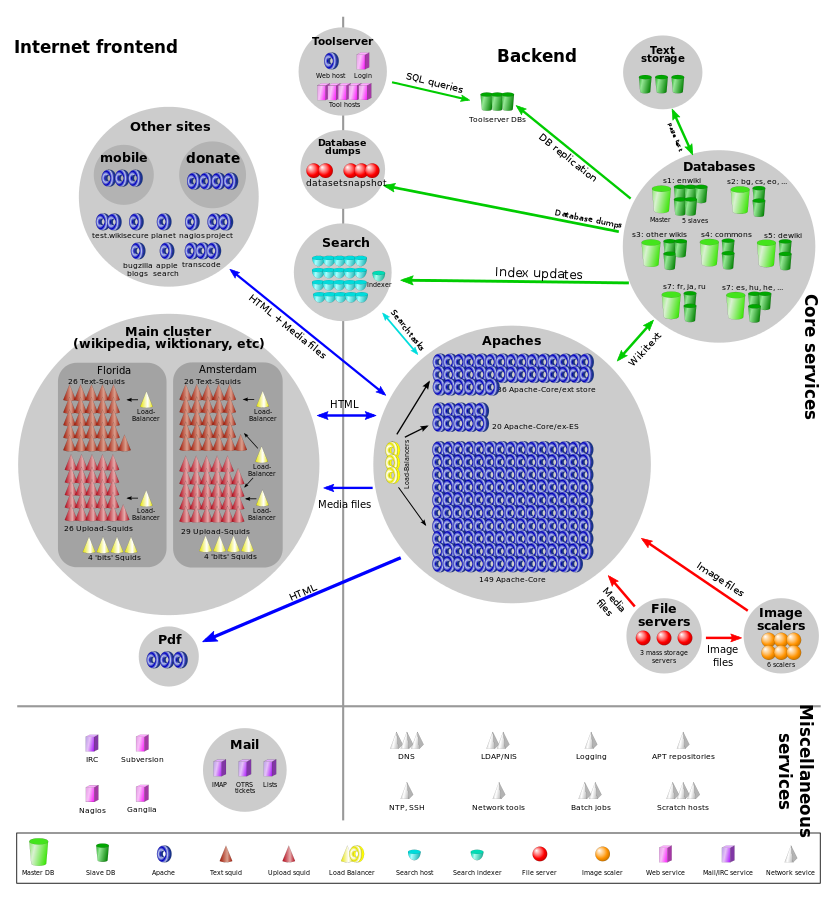
\includegraphics[width=1\textwidth]{Images/servidores_movimento_wikimedia.png}
    \caption{Estrutura dos servidores do Movimento Wikimedia. \citewiki{enwiki_wikimedia_servers_svg}}
    \label{fig:servidores_movimento_wikimedia}
\end{figure}

Os administradores de sistema do Movimento Wikimedia são divididos em três níveis de acesso com permissões distintas: ``\textit{Ops}'', que tem pleno acesso às máquinas da nuvem. ``\textit{Deployment}'', que permite alterar alguns códigos-fonte que rodam nos servidores, e ``\textit{Restricted}'', que podem executar alguns scripts de manutenção e ler os logs dos servidores.

Em setembro de 2020 existem 31 usuários com permissão completa (``\textit{ops}''),  11 com ``\textit{restricted}'' e 55 com acesso de ``\textit{Deployment}''. Dos 31 com acesso pleno, hoje apenas 1 único usuário, ``Ori Livneh'', é voluntário. Todos os outros são funcionários da WMF. Dentre os ``restricted'', novamente encontramos apenas um voluntário em meio a funcionários da fundação, e na categoria ``Deployment'' meia dúzia deles, alguns poucos funcionários da WMDE \footnote{Capítulo alemão do movimento Wikimedia. Estrutura a ser explicada na próxima seção} e dezenas de funcionários da WMF. \citewiki{enwiki_wikimedia_system_administrators}

Esse cenário nos mostra que esta hoje não é uma comunidade como as demais do movimento Wikimedia, compostas em sua vasta maioria por voluntários. Aqui estes são a exceção, e o fato da WMF ser a empregadora de praticamente todos os membros, na prática a coloca em um local de dona das decisões tomadas.

Muitos não veem problemas nesta concentração de poder em um ponto central do movimento, pois as tarefas realizadas por esta comunidade afinal são ``meramente técnicas'' e assim sua composição seria irrelevante, tal como em um ``mito da universalidade e da neutralidade da Ciência pura''. Mito este que segundo Ivan da Costa Marques, ``\textit{prega que o conhecimento científico independe de quem o produziu. Não interessa se o cientista é branco ou negro, mestiço, rico ou pobre, gay, homem, mulher, judeu, muçulmano ou católico, em que século ou região vive ou sob que regime político trabalha, pois a verdade ou o fato científico transcende as contingências locais e sociais e paira acima delas}'' (\cite[p.13]{marques_2005}).

Assim, para o movimento Wikimedia, deve caber aos técnicos ``apenas'' implementar as questões que forem decidas pelas demais comunidades de forma neutra e imparcial, não sendo facultada a esta comunidade a liberdade de ``fazer política''.

Porém, na prática, esta comunidade atua como a principal interface entre os usuários humanos do movimento e os servidores onde são rodados os softwares. Tal como um tribunal superior, está em suas mãos o poder de fazer ou não o que lhe convir, e quando lhe interessar.

Como vimos na seção anterior sobre a crise do captcha, se esta comunidade (ou a WMF, que quase pode ser utilizada como sinônimo aqui pelo alinhamento de interesses) decide que uma decisão local fere os valores do movimento, ela pode simplesmente se negar a implementar a decisão tomada, ou até mesmo se utilizar de meios para reverter alterações que possam ter sido realizadas localmente. Assim como, de forma dura (e que alguns diriam inclusive ditatorial), pode tomar decisões que alterem dinâmicas de funcionamento local e até mesmo encerrem comunidades.

Foi isso o que aconteceu com a Wikipédia em Klingon, em agosto de 2005. Jimbo Wales, um dos fundadores da Wikipédia e o primeiro usuário com permissão ``ops'' nos servidores, fez uma solicitação que fora prontamente atendida por outro ``op'', Brion Vibber, bloquando esta Wikipédia para edição. Brion informou sua ação em um curto e-mail enviando para a lista wikimedia-l: ``\textit{Eu travei a Wikipédia em Klingon (tlh.wikipedia.org) a pedido de Jimmy. Ela continua online por hora, mas não é mais editável}''. \footnote{Tradução livre do original em inglês: ``\textit{I've locked the Klingon Wikipedia (tlh.wikipedia.org) on Jimmy's request. It remains online for now, but is no longer editable.}'' \citewiki{enwiki_wikimedia_klingon_locked}}

Na página do movimento que conta a história da Wikipédia em Klingon podemos ler que Wales ``\textit{nunca declarou publicamente seus motivos para fechar a wiki}'' \footnote{Tradução livre do original em inglês: ``\textit{Jimbo has never publicly stated his exact rationale for closing the wiki}'' \citewiki{enwiki_wikimedia_klingon_history}}, e somos informados de que seu conteúdo, que estava em licença livre, fora migrado para outro servidor de wikis, fora do movimento Wikimedia.

Destino similar teve a Wikipédia em Toki Pona. Como nos conta Bialous (\citeyear[p.171]{bialous_sztuczne_2017}) , ``\textit{as versões em Klingon e Toki Pona da Wikipédia foram retiradas deste site e transferidas para o Fandom, um site de cultura de fãs que também oferece a possibilidade de coletar artigos enciclopédicos no estilo da Wikipédia.}'' \footnote{Tradução com apoio do Google Translate do original em polonês: ``\textit{Wersje Wikipedii w językach klingońskimoraz toki pona zostały wycofane z tego serwisu i przeniesione na Fandom,portal dla kultur fanowskich, dający również możliwość gromadzenia arty-kułów encyklopedycznych na wzór Wikipedii.}}'' Ainda segundo Bialous (\citeyear[p.171]{bialous_sztuczne_2017}), ambas as wikis não contavam com mais de 500 verbetes cada quando foram encerradas no ecossistema da Wikipédia, e talvez pela baixa representatividade de suas comunidades tenha sido tomada a decisão de cima para baixo de encerrá-las.

Em uma rápida consulta aos bancos de dados públicos do movimento, encontramos 11 diferentes Wikipédias que já foram fechadas nesta \textit{wikifarm} (\cite{quarry_close_wikipedias}), que se somam a quatro outras que haviam sido removidas anteriormente ao estabelecimento desta arquitetura de servidores que mantém o registro das wikis desativadas \citewiki{enwiki_wikimedia_list_wikipedias}, totalizando 15 comunidades wikipedistas que foram encerradas pelo movimento global.

O caso das Wikipédias fechadas pode parecer um tanto quanto dramático e extremo, mas serve para ilustrar até qual medida vai o poder daqueles que detém as senhas administrativas dos servidores do movimento. E, como observado por Feitosa (\cite[p.5]{latour_cogitamus_2010} apud), ``\textit{independentemente da intencionalidade ou do controle que o construtor tenha objetivado, sua obra continuará 'oferecendo permissões, possibilidades, concessões', ainda que não previstas ou desejadas, ou seja, continuará fazendo algum tipo de política}''. Assim, na próxima seção iremos explorar mais detalhadamente este modelo de governança global-local do movimento Wikimedia, e daremos mais exemplos desta ``agência política'' da comunidade ``meramente técnica''.



%capítulo 3: de fora para dentro
\chapter{De fora para dentro}

\singlespacing
\begin{flushright}
\textit{"A toda hora,}

\textit{a todo momento}

\textit{De dentro pra fora,}

\textit{De fora pra dentro"}

Walter Franco
\end{flushright}
\doublespacing

Aqui começa o capítulo De fora pra Dentro.  Tenho coisas rascunhadas no drive para trazer para cá.

\section{Estratégias para recepção de novatos.}

"a ampla aceitação de artefatos e arranjos organizacionais é condição sine qua non para participar de uma comunidade de prática (Lave and Wenger 1991, Star 1996). Estranhos e pessoas de fora de um grupo têm a infraestrutura como um alvo de aprendizado. Novos participantes adquirem familiaridade com estes objetos à medida que se tornam membros do grupo. (STAR; RUHLEDER, 1996, apud BOWKER; STAR, 2007, p.35)" (FEITOSA, 2010. p. 17)

# talvez aproveitar originais da fala acima

# Buscar algo do Primo sobre frustração dos entrevistados dada a dificuldade em colaborar no WP. Citar que essa dificuldade foi observada nas falas de lá, e que iremos atrás de falas da Wikipédia organizando nossas atividades.

\subsection{Coisas dentro da Wikipédia}

Seguindo esta trilha então narramos esforços da comunidade wikipedista de melhorar a recepção de novatos, como o Teahouse (MORGAN e HALFAKER, 2018), espaço na Wikipédia anglófona que funciona como um fórum com tutores e usuários novatos, e o Snuggle (HALFAKER et al., 2014), que segundo a Wikipédia (WiKIPEDIA-PT, “Wikipédia:Snuggle”, 07/07/2014) ”é um sistema web para observação e apoio a novatos [...] desenvolvido para permitir que tutores observem as atividades de usuários recém registrados separando novatos desejáveis (boa fé e produtivo (sic)) de indesejáveis (má fé e vândalos)”, a iniciativa "Wikipedia Adventure" (NARAYAN et al., 2017) e o robô ClueBot NG.


# Dificuldade de usuários novos: vários casos de sucesso da TeaHouse na enwiki, mas na ptwiki o "Café dos novatos", que foi renomeado para https://pt.wikipedia.org/wiki/Wikip%C3%A9dia:Tire_suas_d%C3%BAvidas é muito pouco usado e nada linkado.
# Posso comparar número de uso do café na en e na ptwiki


# Falar sobre Wikipedia Adventure (NARAYAN et al., 2017)
# usar (TARABORELLI e CIAMPAGLIA, 2015) 

\subsection{Outreach}

# “Quando os de dentro saem”. Trazer essa fala do Latour para falar de outreach.
# Falar de forma global do programa de educação, atividades glam e editatonas.

Eu diria ## [[citation needed]] que GLAM e Programa de Educação são as duas grandes linhas de outreach do movimento, e a editatona é uma metodologia que é operada por esses e demais tipos de projetos.
-- Mais que isso, a Editatona junta estruturas internas na Wiki com atividades outreach. Ela une os dois mundos. Isso nos chama atenção para ela

# Falar da existência da wiki de outreach. Da tentativa de compartilhamento de experiências, práticas e resultados em um movimento extensionista global e da ferramenta de compartilhamento de Learning Patterns.
# Quando falar de Learning Patterns lembrar de problematizar o conceito de melhores práticas. “Toda prática é surpreendente”. Cukierman ( PASTEUR ? )

\subsubsection{GLAM}

# Catar alguns autores de outreach para falar sobre glam por alto.

# Trazer números. Falar sobre como muitas vezes as atividades GLAM apoiam outros projetos Wikimedia, como Commons, Wikisource e Wikidata.

# Citar o projeto 1lib1ref.
-- Falar que uma das contribuições da pesquisa foi melhoria do código do citation hunt, e sua disponibilização para pt.
--- Trazer números do citation hunt.

# Citar números dos WL* e mencionar que as ferramentas para monitoramento e avaliação foram criadas pela comunidade brasile

\subsubsection{Programa de Educação}

# sobre pré-programa de educação citar interesse da comunidade de engajar acadêmicos e pesquisa (TARABORELLI 2011)

# Falar sobre a história do programa. Quando foi criado, qual sua capilaridade. Quantos cursos em quantos países, bytes adicionados….
    • Estimula professores a proporem para seus estudantes a edição verbetes da Wikipédia como uma atividade da disciplina.
    • Fundação Wikimedia cria materiais de apoio e estimula voluntários a apoiarem as iniciativas como embaixadores.

# Sobre o programa de educação, usar (MARQUES, 2012), (CARVER et al., 2012), (ARCHUBY, 2018), (SOLER-ADILLON, 2018)

…. Programa de Educação, que aconteceu entre 2011 e 2015, onde podemos observar de forma explícita a dificuldade de professores e estudantes para criar conteúdos na Wikipédia e suas tentativas de negociação com a comunidade para a criação de estratégias que possibilitassem a permanência dos conteúdos criados pelos estudantes no projeto.(MARQUES, 2012).
Sabemos que conteúdos criados em editatonas e em salas de aulas costumam ter dificuldades para permanecer na Wikipédia. São comuns os relatos de professores e alunos desmotivados por verem suas contribuições desaparecerem do ar pouco depois de serem salvas. Os casos mais repetidamente vistos como bem sucedidos adotam estratégias para tentar mitigar essa situação, como por exemplo estimular os alunos a editar primeiro em uma página de testes, onde o conteúdo será revisado pelo professor e por outros voluntários, para só então ser adicionado à página do verbete desejado. 

Assim por exemplo foi feito por Juliana Bastos Marques, professora da UNIRIO, responsável pelo primeiro caso de instanciamento do Programa de Educação da Wikimedia Foundation no Brasil. Como relatado por ela na Revista História Hoje (2012, p. 339), "uma maneira bastante segura de evitar conflitos com wikipedistas durante a realização da disciplina é fazer que os alunos escrevam seus artigos apenas em suas páginas de teste, e que após a avaliação eles sejam corrigidos pelo/a professor e embaixadores, para que então possam ser ‘colocados no ar’. Este modelo não é consenso entre os professores que adotaram o projeto até agora, mas se provou fácil e seguro". Corroborando com nossa experiência, a autora afirma no mesmo texto que “observou-se que outros cursos já ministrados no Brasil dentro do mesmo projeto não conseguiram alcançar resultados satisfatórios no mesmo grau" (MARQUES, 2012. p. 338).

# Discussão é rica para quando for falar do programa de educação é sua extensão pro MediaWiki, da necessidade de medir, e da criação de ferramentas para gestão / monitoramento dos cursos.
- Se for falar disso, trazer fala de Zé Marcos. O SI parece feito pensando na demanda de quem está no centro de poder por dados, e não no uso cotidiano dele. Os usuários parecem "perder tempo" preenchendo campos que gerarão relatórios que não são de seu interesse. Pq afinal preencher corretamente então?
# Citar Latour sobre a discussão anterior:
"[...] construir centros implica trazer para eles elementos distantes – permitir que os centros dominem à distância –, mas sem trazê-los "de verdade" [...] Esse paradoxo é resolvido criando-se inscrições que conservarão, simultaneamente, o mínimo e o máximo possível, através do aumento da mobilidade, da estabilidade ou da permutabilidade desses elementos. Esse meio termo entre presença e ausência muitas vezes é chamado de informação. Quando se tem uma informação em mãos, tem-se a forma de alguma coisa sem ter a coisa em si. Como sabemos, essas informações (ou formas, ou formulários, ou inscrições – todas essas expressões designam o mesmo movimento e resolvem o mesmo paradoxo) podem ser acumuladas e combinadas nos centros"(LATOUR, 2000, p. 396)" p. 17

\subsection{As Editatonas}

# Falar aqui que é uma forma de atividade que perpassa atividades de educação, de glam, wiki projetos e outras iniciativas avulsas, inclusive tendo Learning Patterns "próprios", compartilhados por extensionistas de diversas frentes do movimento.

Uma das principais formas que o Movimento Wikimedia tem para engajar e trazer novos/as usuários/as à comunidade são as editatonas. Realizadas por todo o mundo, são eventos onde pessoas se reúnem para editar sobre um mesmo tema de interesse. Como definida pela própria enciclopédia, no verbete ``Maratona de edição'' na Wikipédia em português, uma editatona é um evento ``\textit{durante o qual editores se reúnem para editar e melhorar um tema ou tipo específico de conteúdo, geralmente incluindo um treinamento em edição básica para novos editores. A palavra é uma combinação das palavras ``editar'' (\textit{edit}) e ``maratona'' (\textit{marathon})}'' \citewiki{ptwiki_maratona}.
# Editatonas: falar da ambiguidade do termo em inglês e da perda na tradução.

# trazer foto de uma editatona

Existem variações em seu formato, mas normalmente a atividade começa com um (ou mais) editor/a(es/as) experiente(s) apresentando o funcionamento da enciclopédia e introduzindo suas políticas editoriais. Em sequência, os/as demais participantes criam uma conta de usuário/a e começam a escrever, individualmente ou em grupo, verbetes de seu interesse. Nesta fase, o/a(s) usuário/a(s) experiente(s) atua(m) como tutor/a(es/as), tirando dúvidas dos/as novatos/as que apareçam durante o processo de edição.

Existem também algumas editatonas que funcionam como ``forças-tarefas'' de usuários experientes melhorando verbetes sobre um determinado assunto focal, como por exemplo ``patrimônio natural brasileiro''\footnote{https://pt.wikipedia.org/wiki/Wikipédia:Edit-a-thon/Atividades\_em\_português/Wiki\_Loves\_Earth\_Brasil\_2015 , acessada em 19 de março de 2020.} ou ``eleições no Brasil''\footnote{https://meta.wikimedia.org/wiki/Programa\_Catalisador\_do\_Brasil/2013-2014/Micro-subsídios/Solicitação/Wikitona\_Eleições\_2014 , acessada em 19 de março de 2020.}. Estas atividades dispensam a explanação inicial, e, os/as presentes, editores/as já experientes, partem rapidamente para a divisão de tarefas e escrita de conteúdos. Habitualmente, essas forças tarefas são realizadas online, e a maioria das editatonas presenciais é direcionada em apresentar o mundo wiki a novos/as editores/as a partir de assuntos que sejam de seu interesse.

No início de 2020, a página para divulgação de editatonas da Wikipédia em português já contava com 120 eventos cadastrados desde 2013, sendo 115 deles (98,5\%) realizados no Brasil (\citewiki{ptwiki_edit_a_thon_atividades_portugues}). Já na página para editatonas da Wikipédia em inglês, estavam mapeados 121 eventos, com o primeiro datando de janeiro de 2011 e o último de maio de 2018 (\citewiki{enwiki_how_run_edit_a_thon}), indicando que provavelmente essa comunidade passou a registrar seus eventos realizados no último ano e meio em outro lugar. Já a Wikipédia em espanhol apresentava 92 eventos (\citewiki{eswiki_editaton}), mas aparentemente México, Argentina e Espanha, pólos movimentados de atividade wiki, estão com seus números desatualizados. Terminando nosso passeio pelas páginas sobre editatonas das maiores Wikipédias do mundo, encontramos 60 atividades mapeadas na versão francófona (com destaque para um evento realizado recentemente em Guiné, o primeiro fora do eixo França-Canadá) (\citewiki{frwiki_journées_contributives}) e 83 na enciclopédia em alemão (\citewiki{dewiki_edit_a_thon}).

Se por um lado nossa breve busca não conseguiu números precisos sobre a quantidade de editatonas realizadas pelo mundo, entendemos que os valores encontrados já são suficientes para indicar a relevância deste tipo de evento para o Movimento Wikimedia. Eles também indicam que, além da organização destes eventos ser uma estratégia muito utilizada por todo o mundo, ela é especialmente popular no Brasil.

# Para falar de editatonas citar (CAMPANY e KAHILI-HEEDE, 2018), (FARZAN et al. , 2016), (LITTLEJOHN, Allison et al., 2019), (MARQUES e LOUVEM, 2013)



\section{Organizando nossas editathonas}

A fim de estudar a dificuldade de entrada de novos/as usuários/as \textit{in loco}, em nossa abordagem de pesquisa ``de fora para dentro'', resolvemos organizar nossas próprias editatonas como atividades de campo. Podendo assim observar problemas encontrados pelos/as participantes, e mapear com eles/as os mecanismos de governança da Wikipédia que se apresentam como barreiras, muitas vezes intransponíveis, deixando novatos/as bem intencionados/as sem saber como prosseguir.

Com isto, partindo das observações feitas \textit{in loco} nas editatonas, regressamos a bancada de ciência de dados de nosso laboratório. Nela andamos colados ao banco de dados, realizando inferências nos dados abertos da Wikipédia. Investigamos padrões, elementos e comportamentos da governança da comunidade que interagiram com nossos participantes durante e após as editatonas.

\subsection{Por que resolvemos fazer editatonas?}

*** talvez falar também sobre a escrita dos 3 verbetes sobre autores CTS. ## Pegar notas e citações no card do Trello sobre trabalho do Esocite. ver https://trello.com/c/y6cDtTZi/290-adicionar-sobre-trabalho-do-esocite-no-cap%C3%ADtulo-4

A metodologia adotada de realizar editatonas foi validada como pertinente logo no início da pesquisa em 2017, com a realização de uma atividade em sala de aula com a turma de pós-graduação da disciplina ``\textit{Estudos CTS (Ciências-Tecnologias-Sociedades): aproximações brasileiras e latino-americanas}'', ministrada no Programa de Engenharia de Sistemas e Computação da COPPE/UFRJ, no 2º período de 2017. Atividade esta que teve seus resultados retratados no trabalho ``\textit{Práticas de escrita biográfica na Wikipédia em português em turmas de pós-graduação}'', apresentado no VII Simpósio Nacional de Ciência, Tecnologia e Sociedade (Esocite.BR), também em 2017 (\cite{andrade_historias_2017}).

A editatona foi realizada durante uma aula em que o professor não poderia estar presente, e os/as estudantes deveriam se auto organizar e autogerir para realizar alguma atividade. Inicialmente o grupo imaginava que iria trabalhar no CTS Brasil Blog, site idealizado para escoar produções feitas ao longo do curso. Mas, no momento do encontro, percebeu-se que a produção deste já tinha seu fluxo de trabalho remoto bem definido, e que as horas que teríamos juntos presencialmente poderiam ser melhor aproveitadas de outra forma.

Assim, com a decisão de realizarmos uma editatona, fiz uma apresentação sobre o funcionamento da Wikipédia e suas políticas editoriais. Propus então para o grupo que o escopo da atividade fosse o desenvolvimento de verbetes biográficos sobre os autores CTS que estávamos estudando\footnote{No capítulo 4 detalhamos as práticas de escrita biográfica que já estavam ocorrendo durante a disciplina.}. O grupo então debateu sobre quais verbetes editar, e entendendo que existia um artigo que precedia os biográficos em importância para divulgação do tema CTS, definiu que seria feita uma força tarefa para melhorar apenas um verbete: ``\textit{Estudos de ciência, tecnologia e sociedade}''. Os 13 presentes então se dividiram em grupos, responsáveis por criar/melhorar diferentes seções do verbete em paralelo, que somadas comporiam a nova versão do verbete ao final da aula.

Antes da atividade, o verbete contava com 3.989 bytes\footnote{Unidade de medida utilizada pela comunidade para medir o tamanho de revisões e verbetes.}, com uma breve introdução e uma seção textual intitulada ``Ensino'', seguida por seções de ``Bibliografia'' e ``Ligações externas''. Três horas depois, o texto já apresentava 23.570 bytes, sendo 20.281 bytes adicionados pela turma e 18 bytes adicionados pelo usuário FSogumo, que não era aluno do curso e adicionou, durante a atividade, o \textit{template} de geração automática de referências ao verbete, que agora contava com dez seções textuais diferentes.

Sabendo da dificuldade tão relatada de conteúdos criados em salas de aula persistirem por um longo período de tempo na Wikipédia (\cite{marques_trabalhando_2012}), (\cite{carver_assigning_2012}), (\cite{archuby_experiencias_2018}), (\cite{soler-adillon_wikipedia_2018}), voltamos então ao verbete ``\textit{Estudos de ciência, tecnologia e sociedade}'' um mês depois da realização da atividade, para pesquisar o que teria acontecido com as edições de nossos/as editores/as.

Encontramos mais três edições feitas por alunos da turma no verbete após a atividade, adicionando mais 10.551 bytes, e percebemos uma situação que contradiz toda a literatura sobre editatonas: nenhuma edição de nossa turma havia sido revertida, e todo o conteúdo criado por nossos/as novos/as editores/as continuava no ar. Este fato é ainda mais surpreende pois em nossa atividade os/as estudantes foram estimulados/as a editar diretamente a Wikipédia, sem realizar uso prévio das páginas de testes, o que diminuiria ainda mais as chances de sobrevivência de seus conteúdos (\cite{marques_trabalhando_2012}).

Perante tão distinta situação, resolvemos então investigar o que havia acontecido de especial em nossa editatona, e enredamos a ferramenta \textit{Objective Revision Evaluation Service} (ORES)\footnote{Em português Sistema Objetivo de Avaliação de Revisões.}, para analisar todas as edições feitas durante a atividade.

O ORES é uma ferramenta de inteligência artificial que avalia edições (também chamadas pelos/as usuários/as de revisões) feitas nas Wikipédias. Solicitamos aqui de nossos/as leitores/as a gentileza de aceitar o ORES como uma caixa-preta (assim como ela é aceita pelos/as editores/as e reversores/as das Wikipédias)\footnote{Na verdade no uso cotidiano da enciclopédia o ORES faz parte das redes que sustentam outras caixas pretas, enquanto ele fica invisível fazendo suas avaliações no backend e seu nome permanece desconhecido para a maior parte da comunidade.}, e tomemos suas saídas como avaliações confiáveis sobre as edições apreciadas. Para cada edição, o ORES nos indica probabilidades de ser danosa, feita em boa fé e de ser revertida (``apagada'').

\begin{center}
\begin{table}
\begin{tabular}{ |c|c|c|c| } 
 \hline
\textbf{Id da Edição} & \textbf{Não danosa} & \textbf{Feita em boa fé} & \textbf{Deve ser revertida} \\
\hline
49529742 & 76\% & 87\% & 65\% \\
\hline
49529756 & 76\% & 90\% & 33\% \\
\hline
49529775 & 52\% & 59\% & 71\% \\
\hline
49529792 & 36\% & 35\% & 76\% \\
\hline
49529803 & 80\% & 84\% & 58\% \\
\hline
49529830 & 58\% & 61\% & 73\% \\
\hline
49529836 & 24\% & 34\% & 76\% \\
\hline
49529856 & 42\% & 56\% & 69\% \\
\hline
49531419 & 54\% & 63\% & 72\% \\
\hline
\textbf{49531652} & \textbf{98\%} & \textbf{99\%} & \textbf{04\%} \\
\hline
49781518 & 91\% & 96\% & 12\% \\
\hline
49785059 & 86\% & 88\% & 41\% \\
\hline
49802969 & 67\% & 88\% & 32\% \\
\hline
Média & 64\% & 72\% & 52\% \\
 \hline
\end{tabular}
\caption{Avaliação feita pelo ORES de todas as edições feitas na atividade, com a edição do coordenador destacada em negrito.}
\label{table:avaliacao-ores}
\end{table}
\end{center}

A tabela \ref{table:avaliacao-ores} exibe a avaliação do ORES para todas as edições feitas no contexto de nossa editatona, começando da mais recente e descendo cronologicamente. Observando a tabela podemos notar que a maioria de nossas edições foram vistas pelo sistema tanto feitas em boa fé como não danosas, mas apresentavam percentual alto de chances de serem revertidas.

Não por acaso, esse é exatamente o perfil de edição que organizadores de editatonas relatam vivenciar. Seus/suas colegas estão editando em boa fé e realizando alterações que não são danosas para a enciclopédia, mas a falta de um determinado padrão de escrita, esperado pela comunidade, faz com que as edições sejam revertidas.

Ao observarmos atentamente a tabela criada pelo ORES uma edição nos salta aos olhos. A edição com id \textbf{49531652} apresenta 98\% de chances de não ser danosa, 99\% de ser feita em boa fé e apenas 4\% de chances de ser revertida. Ao clicar no detalhamento desta edição, podemos ver que ela havia sido feita pelo usuário experiente que coordenava a atividade (eu), e, nesta edição de 839 \textit{bytes}, todos os conteúdos criados nas edições anteriores eram revisados, sendo colocados no formato wikipédico, com ligações internas e referências no padrão wiki.

Esta edição específica, além de auxiliar a manter na enciclopédia os conteúdos que, segundo o ORES, tinham grandes chances de serem revertidos, estrutura o verbete e ajuda os próximos editores a criarem conteúdos mais ``aceitáveis'' para enciclopédia. As três edições seguintes a essa, feitas por alunos da turma, observam suas chances de serem revertidas caírem drasticamente. Antes da edição do coordenador da atividade, as edições dos novatos apresentavam em média 65,88\% de chances de serem revertidas. Já as realizadas por esse mesmo recorte de usuários/as posteriormente apresentam uma enorme queda nesse valor, para apenas 28,33\%.

Percebemos, então, a importância do coordenador da atividade não ser um mero tutor que orienta os participantes e apresenta dicas de edição. Sua participação ativa na escrita coletiva dos mesmos verbetes que os/as editores/as novatos/as estiverem trabalhando pode auxiliar a manter as edições destes/as no ar, aumentando o sucesso da atividade tanto na satisfação dos participantes, como na disponibilização de mais conteúdos livres a longo prazo.

Após a alta frequência de edições feitas pela turma em agosto e setembro de 2017, a página ``\textit{Estudos de ciência, tecnologia e sociedade}'' voltou a ser pouco editada. Nos dois anos seguintes, até o final de 2019, foram feitas apenas duas contribuições com adição substancial de conteúdo, que não dialogaram com o conteúdo criado pela turma, mas criaram uma seção sobre o ``movimento CTSA (Ciência, Tecnologia, Sociedade e Ambiente)''. Essas edições adicionaram 1415 bytes ao verbete, que permaneceram no ar não revisados nem contestados até o início de 2020.

Esse baixo volume de revisões no verbete mostra a importância das editatonas para não apenas apresentar o funcionamento da Wikipédia buscando engajar novos/as editores/as, como também para produzir conteúdos em assuntos que não sejam muito populares entre os/as editores/as habituais. Apesar de suas mais de 200 mil edições por mês, a Wikipédia tende a concentrar seu maior volume de edições em tópicos como política, esportes ou televisão.

\begin{center}
\begin{table}
\begin{tabular}{ |c|c| } 
 \hline
\textbf{Verbete} & \textbf{Edições em 2019} \\ 
\hline
Big Brother Brasil 19 & 581 \\ 
\hline
Governo Jair Bolsonaro & 357 \\ 
\hline
Copa São Paulo de Futebol Júnior de 2019 & 265 \\ 
\hline
Rompimento de barragem em Brumadinho & 247 \\ 
\hline
Primeira Liga de 2018–19 & 217 \\ 
\hline
Copa da Ásia de 2019 & 197 \\ 
\hline
Campeonato Mundial de Handebol Masculino de 2019 & 182 \\ 
\hline
Lista de participantes do Big Brother Brasil & 173 \\ 
\hline
Verão 90 & 168 \\ 
\hline
Temporada do Sport Club Corinthians Paulista de 2019 & 163 \\ 
 \hline
\end{tabular}
\caption{Lista de verbetes mais editados em 2019 na Wikipédia em português.}
\label{table:verbetes-mais-editados-2019}
\end{table}
\end{center}

Assim, conteúdos criados em editatonas que tenham como temática assuntos não midiáticos tendem a não receber muitas colaborações posteriores, e a produção gerada na atividade tenderá a se estabilizar como o conteúdo que futuros leitores terão acesso em suas pesquisas. Cabe dar bastante ênfase aqui ao fato de que, ao contrários de trabalhos científicos, que ``\textit{a maioria nunca é lida por ninguém}'' (\cite[p.59]{latour_ciencia_1987}), os artigos criados na Wikipédia tem uma grande audiência. E, quanto mais conteúdos tenha um verbete, mais facilmente ele será encontrado por robôs e indexado por mecanismos de busca, fazendo com que ainda mais leitores encontrem o texto.

Com isso, quando uma editatona expande um verbete, além de estar melhorando a qualidade daquele conteúdo para a audiência esperada, ela está também aumentando o público que terá acesso àquele verbete.

\begin{figure}[H]
    \centering
    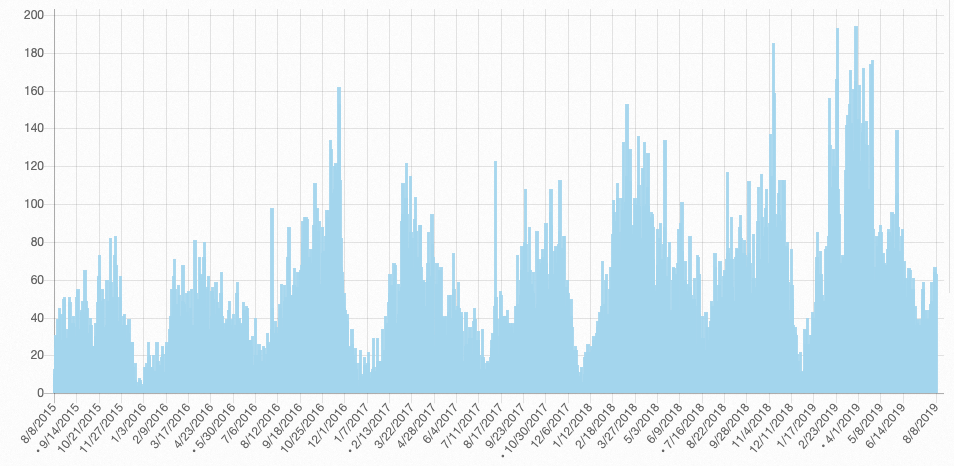
\includegraphics[width=1\textwidth]{Images/acessos-estudos-cts.png}
    \caption{Acessos ao verbete trabalhado dois anos antes e dois anos depois da atividade.}
    \label{fig:acessos-estudos-cts}
\end{figure}

Na figura \ref{fig:acessos-estudos-cts} observamos os acessos ao verbete ``\textit{Estudos de ciência, tecnologia e sociedade}'' entre 8 de agosto de 2015 e 8 de agosto de 2019, exatamente dois anos antes e dois anos depois da editatona. Diferente do trabalho apresentado em 2017 (\cite{andrade_historias_2017}), que observara dois meses antes e dois meses depois da atividade, optamos por esse recorte maior de tempo para dar conta da sazonalidade observada nos acessos ao verbete ao longo do ano, que parece ser bastante influenciada pelo calendário escolar anual.

Compreendido então o recorde, observamos que, nos dois anos anteriores à editatona, o verbete apresentava uma audiência média de 38 acessos por dia. Nos dois anos seguintes, esse número cresce 55,26\%, para 59 acessos diários.

Em valores absolutos, e considerando que o verbete manteria um volume estável de visitas com seu conteúdo anterior\footnote{Consideração benevolente, pois entre 2016 e 2019 os acessos à Wikipédia em português como um todo caíram 1,5\%, como pode ser visto em https://stats.wikimedia.org/\#/pt.wikipedia.org/reading/total-page-views/normal|bar|2016-01-01~2020-01-01|~total|monthly , acessada em 19 de março de 2020.}, isso significa que a editatona de 3 horas, com 13 participantes, proporcionou em dois anos 15.330 leituras a mais sobre ``Estudos de ciência, tecnologia e sociedade'' em português.

Perante o volume de acessos da Wikipédia, aproximadamente 13 milhões por dia somente em português, essas 15 mil leituras em dois anos podem parecer poucos relevantes. Mas, dentro de seu nicho específico de um assunto não muito midiático como ``Estudos de ciência, tecnologia e sociedade'', esse número significa que, no mundo real, 15 mil pessoas que antes não teriam encontrado esse conteúdo em português sobre o tema agora o terão, e com encontrando um texto enciclopédico com maior abrangência e mais referências do que eram apresentadas antes da editatona.

A título de comparação, podemos olhar para os números de outra atividade desenvolvida pela mesma turma: o ``CTS Brasil Blog''\footnote{Disponível em https://ctsbrasilblog.wordpress.com/ .}. Ao longo de todo o curso, os/as estudantes criaram conteúdos e os publicaram nesta página, dedicada especialmente a ``\textit{circular vídeos, resenhas, entrevistas, manifestos e o que mais sair das digestões feitas durante a disciplina}'' (\cite{cts_brasil_blog}). Ao final do curso, o site contava com 17 publicações, feitas por 10 autores/as diferentes.

No ano de sua criação o blog teve seu pico de acessos, muito provavelmente ocasionado pelas visitas dos/as próprios/as estudantes-autores, com 526 visitas. No ano seguinte, este número cai para 215 e, em 2019, o blog encerra o ano com 149 visualizações. Enquanto o volume de acessos inicial pode ser explicado pelos autores acessando o site durante a disciplina, pois só nos dois primeiros meses de vida o \textit{site} recebeu 482 visualizações, os meses seguintes de novembro e dezembro somados totalizam 44 visitas. Podemos então considerar que em outubro de 2017 o blog é estabilizado por seus/suas autores/as, que param de publicar após o término da disciplina, e que os acessos que acontecem a partir daí seriam feitos por leitores/as alheios ao curso. Assim, considerando todos os acessos dos dois últimos meses de 2017, e os anos inteiros de 2018 e 2019, no que podemos considerar leituras orgânicas\footnote{Em mídias sociais, esse é o termo utilizado para acessos feitos sem pagamento de divulgação, por usuários que encontram o site através de links externos ou buscadores.} do conteúdo, temos um volume de 408 visualizações, em uma média de 0.51 visitas por dia.

\begin{figure}[H]
    \centering
    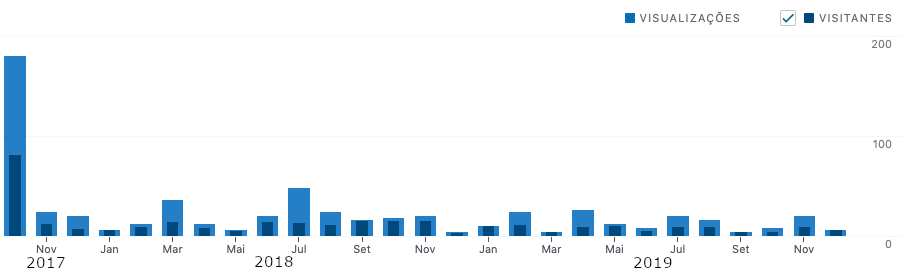
\includegraphics[width=1\textwidth]{Images/acessos-cts-brasil.png}
    \caption{Acessos ao CTS Brasil Blog por mês.}
    \label{fig:acessos-cts-brasil}
\end{figure}

Essa iniciativa do CTS Brasil Blog é claramente um caso de sucesso de divulgação científica, que continua no ar até hoje apresentando para leitores lusófonos, e em grande maioria (89,3\%, como pode ser visto na figura \ref{fig:acessos-geo-cts-brasil}) do Brasil, conteúdos sobre os Estudos de Ciências-Tecnologias-Sociedades, que outrora ficariam restritos às salas de aula de pós-graduação. Mas, seu relevante volume de acessos parece pequeno se comparado às mais de 15 mil visitas que receberam os conteúdos criados na editatona realizada pela mesma turma.\footnote{É importante destacar que o blog aceitava diferentes tipos de conteúdos, e não apenas textos enciclopédicos. Aqui comparamos seus acessos não para medir qual atividade teve maior sucesso, mas apenas para colocar o alcance da atividade realizada na Wikipédia em perspectiva.}

\begin{figure}[H]
    \centering
    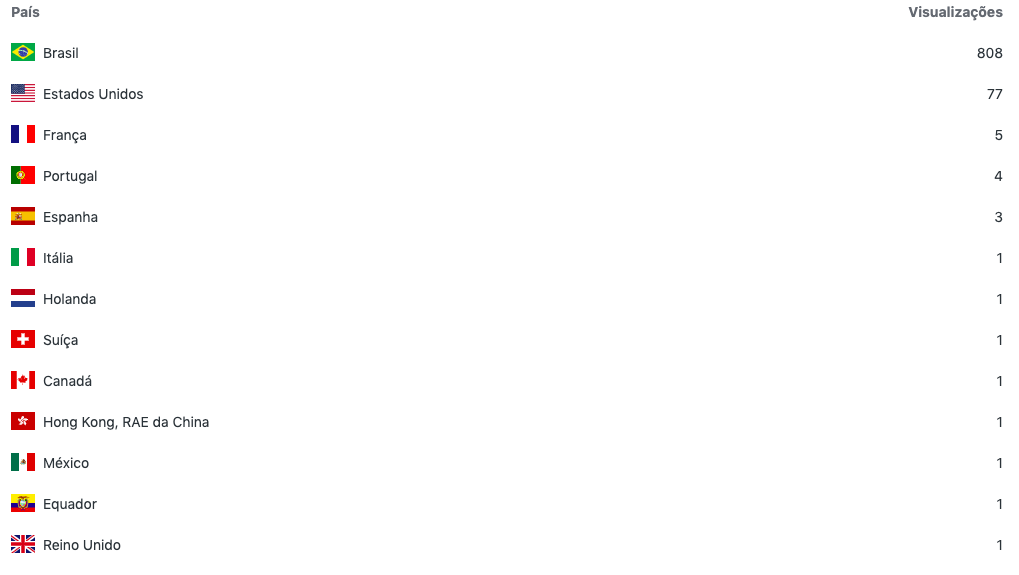
\includegraphics[width=1\textwidth]{Images/acessos-geo-cts-brasil.png}
    \caption{Acessos Geolocalizados ao CTS Brasil Blog.}
    \label{fig:acessos-geo-cts-brasil}
\end{figure}

Tendo em mente estes casos de sucessos na criação de conteúdos, que são de fato lidos pela sociedade além dos muros da universidade, decidimos que convidaríamos para participar das editatonas de nossa pesquisa as redes que orbitam o Laboratório de Informática e Sociedade (LabIS) da COPPE/UFRJ, fazendo com que nosso trabalho de campo tenha um efeito colateral um tanto quanto interessante: enquanto estudamos os mecanismo de governança da Wikipédia, criamos conteúdos livres em português sobre assuntos relacionados a Ciências-Tecnologias-Sociedades locais, tais como moedas sociais, softwares para acessibilidade, educação popular, informática e educação, mobilização política em redes sociais e demais assuntos que interessarem aos participantes das atividades. Promovemos assim maior acesso de leitores/as do idioma português, por todo o mundo, a esses conteúdos muitas vezes ignorados nos meios de divulgação científica e marginalizados por grande veículos de comunicação.

\subsection{Preparando nossas editatonas}

Nossa pesquisa tinha como objetivo organizar editatonas presenciais para tanto acompanhar in loco, com o olhar míope da formiga, como as interações entre novatos e enciclopédia acontecem, como para disponibilizar livremente em páginas bastante visitadas conteúdos sobre assuntos relacionados a pesquisas do campo CTS e correlatos.

A ideia de organizar editatonas fora validada de forma ad hoc em uma atividade realizada no início da jornada do autor neste curso de mestrado, dentro de uma disciplina oferecida em 2017, antes mesmo do projeto desta tese ter tomado seu recorte atual.

\subsubsection{utilizando Learning Patterns}

Nos preparativos para a realização desta editatona estudamos diversas outras já realizadas, conforme explicitado na seção anterior, e performamos uma extensa revisão bibliográfica dos chamados Learning Patterns da comunidade Wikimedia.

\begin{figure}[H]
    \centering
    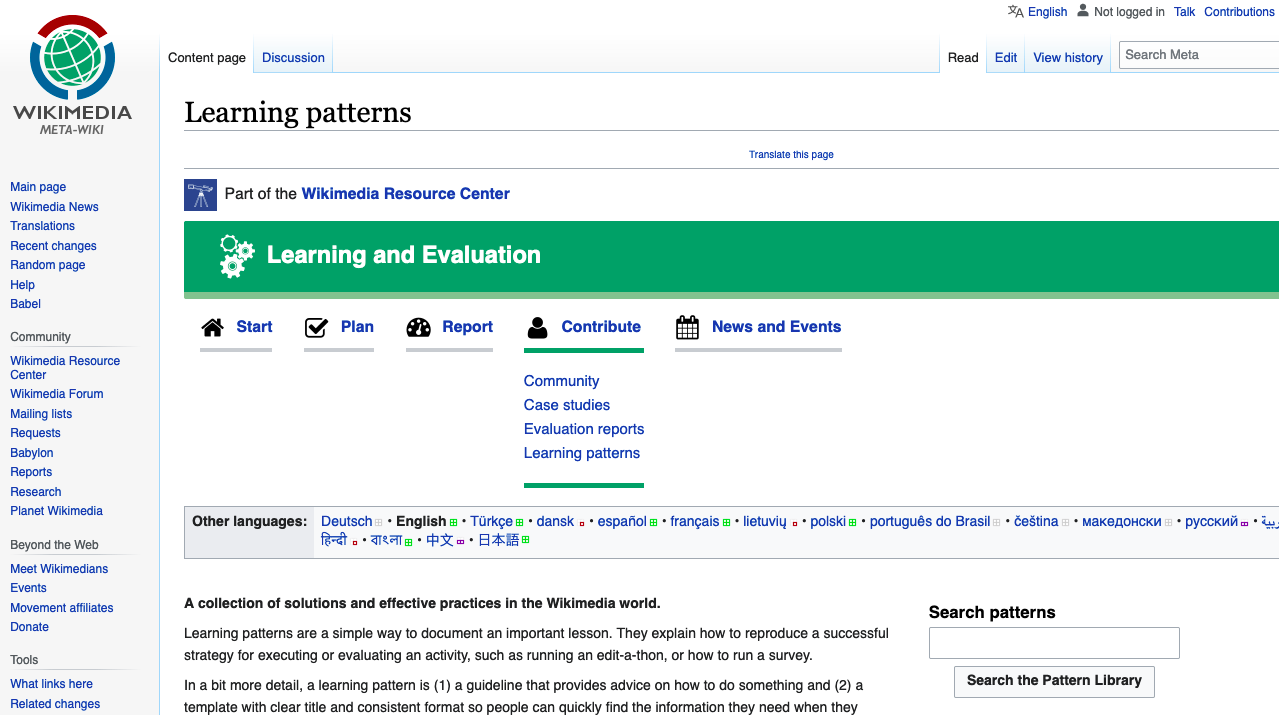
\includegraphics[width=1\textwidth]{Images/learning_patterns.png}
    \caption{Portal de Learning Patterns do movimento Wikimedia.}
    \label{fig:learning_patterns}
\end{figure}

*** Falar da existência da wiki de outreach. Da tentativa de compartilhamento de experiências, práticas e resultados em um movimento extensionista global e da ferramenta de compartilhamento de Learning Patterns.
*** Quando falar de Learning Patterns lembrar de problematizar o conceito de melhores práticas. “Toda prática é surpreendente”. Cukierman ( PASTEUR ? )

*** versar sobre learning patterns criados pela comunidade que foram lidos para a confecção do roteiro. Ver https://trello.com/c/t9SxjmTz/253-encontrar-dados-sobre-learning-patterns-utilizados

*** catar referência sobre o projeto de learning patterns

*** Quando falar de Learning Patterns lembrar de problematizar o conceito de melhores práticas. “Toda prática é surpreendente”. Cukierman

*** Dar números de quantos learning patterns foram lidos neste levantamento.

*** Citar explicitamente os learning patterns utilizados para criar nosso roteiro. Tenho isso mapeado em algum lugar, não sei se no drive ou no trello.

\subsubsection{Criando nosso Learning Patterns}

*** Falar do roteiro criado...ver https://trello.com/c/dH13LfQh/466-detalhar-a-cria%C3%A7%C3%A3o-do-meu-roteiro-da-organiza%C3%A7%C3%A3o-de-uma-editatona
*** ver cards no trello da coluna "o que fazer a cada editatona". Falar de dados, prazos, emails convite...

Seguindo a trilha dos learning patterns estudados, criamos predefinições\footnote{Predefinições são página do MediaWiki que funcionando como templates, podendo ser importadas para outras páginas trazendo automaticamente uma estrutura previamente determinada.} para facilitar a utilização das páginas de testes pelos participantes das editatonas. Estas predefinições permitiram com facilidade a criação e listagens de novas subpáginas de testes, tarefa nada trivial para um usuário não habituado ao funcionamento do MediaWiki.

\begin{figure}[H]
    \centering
    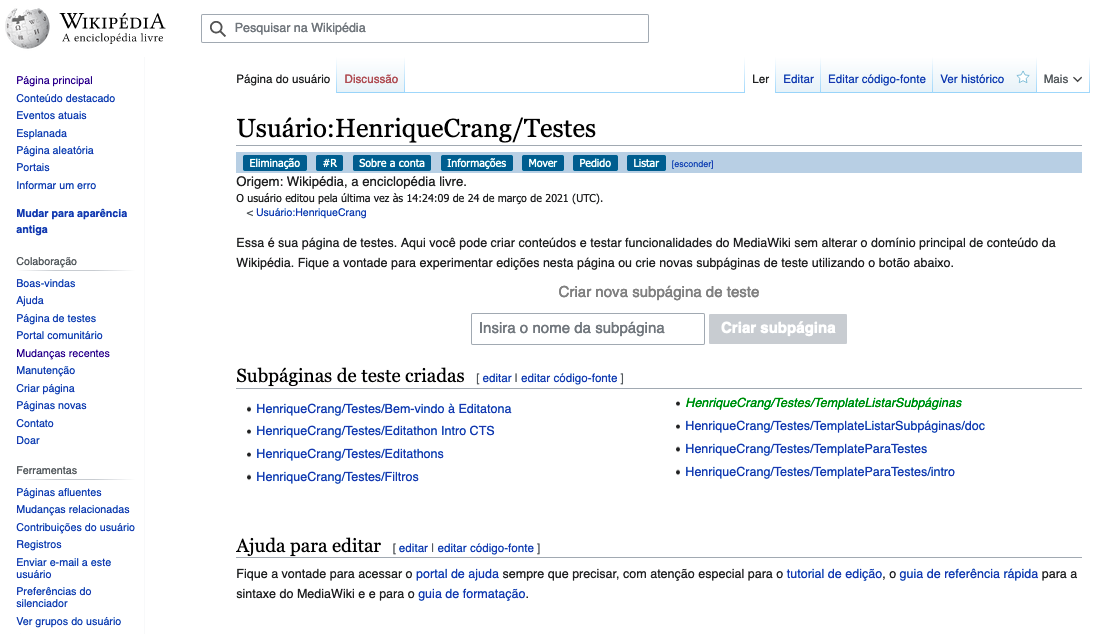
\includegraphics[width=1\textwidth]{Images/pagina_de_Testes.png}
    \caption{Página de testes criada utilizando a predefinição desenvolvida pela pesquisa.}
    \label{fig:pagina_de_testes_editatona}
\end{figure}


*** Sobre Criação de pré-definições... ver https://trello.com/c/Mp3HXAPg/187-documentar-trabalho-feito-criando-pr%C3%A9-defini%C3%A7%C3%B5es

*** Usar mais prints para mostrar as pre-definições


A predefinição se chama "Predefinição:Página de testes do usuário", e atualmente é utilizada por XX usuários da Wikipédia em português. \footnote{Como pode ser visto em https://pt.wikipedia.org/wiki/Especial:Páginas_afluentes/Predefinição:Página_de_testes_do_usuário, acessada em }

\subsection{Colocando o plano em prática}

***  Falar aqui da primeira editatona, feita presencialmente em 21 de novembro de 2019.

\begin{figure}[H]
    \centering
    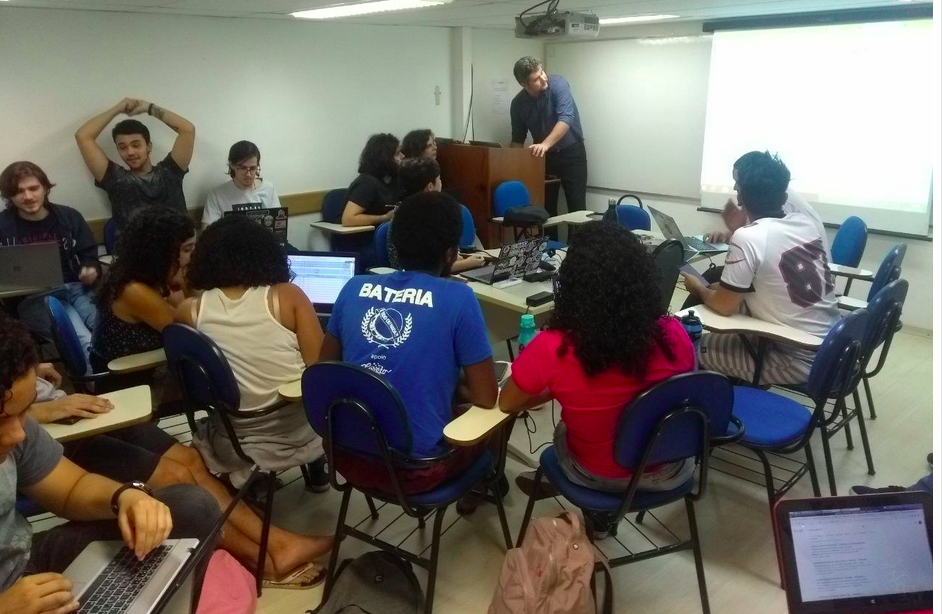
\includegraphics[width=1\textwidth]{Images/editatona_presencial.png}
    \caption{Editatona presencial com turma de graduação no dia 21 de novembro de 2019.}
    \label{fig:editatona_presencial}
\end{figure}

***  Trazer alguns poucos números dela, e concluir dizendo que essa foi a única realizada seguindo o mapa original, pois a realidade se mostrou mais realista que o plano, e desvios e adaptações foram necessários para que a pesquisa continuasse em um mundo que mudou da noite para o dia


\subsubsection{No meio do caminho tinha uma pandemia}

Após a validação de nosso roteiro com a editatona realizada ao final de 2019, nos planejamento para realizar diversas atividades no início do primeiro semestre letivo de 2020. Porém, o mundo foi surpreendido pela pandemia de COVID-19, que se apresentou acompanhada de medidas de isolamento social que inviabilizaram a realização de mais atividades presenciais conforme planejado.

"em qualquer caso de trabalho acadêmico, os planos de pesquisa sonhados pelo pesquisador têm poucas chances de serem realizados em sua totalidade." (GONÇALVES, 2016. p. 18)

*** atividades foram adiadas duas três vezes... passado um tempo, percebemos que não era uma mera questão de adiar o plano, mas de o alterar para dialogar com essa nova realidade que se impôs.

Assim, nossa pesquisa encontrou um bloqueio, e se viu obrigada a buscar desvios negociando com o vírus SARS-CoV-19, com as políticas públicas de isolamento social, com softwares de videoconferência e com redes de engajamento popular à distância para construir novas composições e seguir, se não para o rumo previsto originalmente, mas para um novo que apontasse para um norte (ou seria sul?) próximo à discussão proposta no trabalho.

Partimos então para a criação de uma nova metodologia de realização de editatonas com novatos, que pudesse ser realizada à distância. Conforme já mencionado, tradicionalmente as editatonas focadas em novatos são realizadas presencialmente e os eventos à distância reúnem editores experientes. Desta forma, toda a literatura existente sobre editatonas à distância não nos foi de muita valia, por suas metodologias sempre partirem do princípio de que os participantes já dominam o funcionamento do MediaWiki e as políticas editoriais da Wikipédia.

Subitamente percebemos que nossa pesquisa ganhara uma nova dimensão e responsabilidade: caberia a nós propormos e testarmos uma metodologia nova para a realização de editatonas para editores novatos à distância. Debruçamo-nos então sobre este desafio e passamos a testar diversas ferramentas de realização de encontros virtuais e a frequentar eventos online organizados por diversas instituições para encontrarmos exemplos e inspirações.

*** necessidade de tradução, translação..sabemos que traições acontecerão no processo, mas buscamos o máximo de fidelidade ao propósito e à propiciar dinâmicas entendidas como interessantes.

Uma das características marcantes das editatonas presenciais com novatos é a escrita em conjunto, no mesmo teclado, de textos. Pequenos grupos de 2 a 4 pessoas se formam em torno de um computador e, juntos, os participantes enfrentam os desafios de escrever verbetes enciclopédicos pela primeira vez. Como seria possível mimetizar esta experiência virtualmente? Como no mundo online, mesmo estando todos na mesma sala virtual, é possível a formação de pequenos que dialogam entre si, sem que a conversa de cada grupo atrapalhe os demais?

Em salas convencionais de videoconferência esta prática seria inviável. Diferente de uma sala do mundo físico, onde diferentes pessoas podem falar ao mesmo tempo para grupos diferentes e todos serem compreendidos, em uma sala virtual é imprescindível que apenas um participante fale por vez, sob pena do encontro se tornar uma cacofonia incompreensível.
Cogitamos então criar várias salas virtuais, dividir os participantes em grupos e pedir para que cada um se dirigisse a um link diferente após uma abertura realizada em uma única sala. Porém, não estávamos confortáveis com esta solução. A necessidade de abrir uma nova conexão durante a atividade parecia algo um tanto quanto desmobilizante, e que criaria uma segregação entre os grupos impedindo uma série de dinâmicas interessantes de colaboração e circulação observadas em editatonas presenciais.

Umas das dinâmicas que se perderiam seria a troca de grupo. É normal um novato querer circular pela sala em uma editatona. A pessoa pode começar em um grupo, mas durante a editatona se engajar em outra atividade. Algumas vezes este movimento acontece pois a pessoa escuta, de rabo de ouvido, algum comentário vindo de outro grupo que a faz querer contribuir com outra tarefa.

Outra dinâmica muito dificultada pela segregação das salas seria o apoio do wikipedista experiente. Em editatonas presenciais, ele roda entre os grupos, apoiando e tirando dúvidas, e pode a qualquer momento ser chamado por um grupo que necessite ajuda. Mesmo que o usuário experiente tivesse acesso aos links de todas as diferentes videoconferências e ficasse pulando de sala em sala, como um grupo que precise de ajuda em um determinado instante poderia chamá-lo? Seria necessário utilizar outra ferramenta, como o telefone por exemplo, ou o grupo precisaria aguardar mais alguns minutos para a aparição surpresa do tutor em sua sala virtual, tal qual um enfermo acamado agoniadamente aguarda pela rara ronda médica.

Ademais, em editatonas presenciais não são incomuns momentos em que o wikipedista experiente, a partir da dúvida de um grupo específico, compartilha com todos os presentes alguma situação que o grupo tenha vivido, explicando a questão para todos e dando dicas sobre como prosseguir quando a mesma barreira porventura for encontrada por qualquer dos participantes.

A possibilidade de inviabilizar todas as dinâmicas narradas acima nos causou grande inquietação, pois sentíamos que a editatona virtual que estávamos criando não seria capaz de oferecer uma boa experiência aos participantes.

\subsubsection{Encontrando uma tradução viável}

Em nosso esforço para traduzir a metodologia de editatonas presenciais para novatos ao mundo virtual, sem que as traições que inevitavelmente aconteceriam no processo inviabilizassem a atividade, enxergamos uma luz ao fim do túnel quando testamos a ferramenta Discord.

O Discord é um serviço de comunicação online que oferece ferramentas de interação em texto, áudio e vídeo, assim como compartilhamento de tela, e pode ser acessado tanto através de seu aplicativo próprio como através de um webapp em seu site. Criado em 2015 pela produtora de jogos virtuais Hammer \& Chisel, se tornou rapidamente muito popular entre gamers e, com sua popularidade, passou a ser utilizado por outras comunidades e grupos de interesse, ultrapassando em meados de 2019 a marca de 250 milhões de usuários. (SHERR, 2019)

Ao testarmos o Discord uma diferença marcante para outras ferramentas de reuniões virtuais saltou aos olhos: seus espaços de encontro não são orientados a salas, mas a “servidores". No contexto do uso da ferramenta, o termo “servidor” significa um ambiente virtual ao qual os usuários se conectam, e dentro dele podem existir várias salas, tanto de texto como de áudio/vídeo. Estando em um servidor, qualquer usuário consegue navegar por todas as salas de texto sem precisar abandonar a sala áudio/vídeo em que estiver no momento, podendo também, se desejar, trocar de sala multimídia automática e imediatamente com apenas um clique.

\begin{figure}[H]
    \centering
    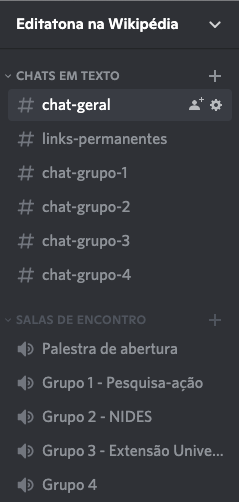
\includegraphics[width=0.5\textwidth]{Images/discord_channels.png}
    \caption{Estrutura das salas criadas no servidor “Editatona na Wikipédia” no Discord.}
    \label{fig:estrutura_discord}
\end{figure}

 O dinamismo possibilitado pelo Discord nos deixou esperançosos, e partimos para a criação e personalização de um servidor lá para nossas atividades. Criamos inicialmente cinco salas multimídias, que na interface do sistema rebatizamos de “Salas de encontro”. A primeira chamada “Palestra de abertura”, onde todos os participantes deveriam se encontrar no início da atividade, e as salas seguintes com nomes como “Grupo 1”, com o numeral sendo incrementado a cada sala nova.
 
 Para as salas de texto, chamadas na interface de “Chats em texto” criamos inicialmente seis. Uma com o mesmo nome de cada grupo, uma intitulada “chat-geral” e por fim uma chamada “links-permanentes”, onde somente o organizador poderia enviar mensagens.
 
 Em torno desta estrutura foi criada a seguinte metodologia para desenvolvimento da atividade: todos os usuários, nos convites enviados para a atividade, foram orientados a entrar na sala “Palestra de abertura” assim que acessassem o servidor. Lá, o wikipedista experiente faria uma apresentação de no máximo meia hora sobre a Wikipédia, introduzindo suas políticas editoriais e a interface do sistema MediaWiki. Após a apresentação, os usuários seriam convidados a acessar o chat “links-permanentes”, clicarem em “Criar uma conta”, e depois informarem no “ chat-geral” seu nome de usuário.
 
 Vencido o primeiro contato com a Wikipédia, os participantes então eram convidados a acessar a página criada para organizar os esforços daquela editatona, com link disponível no chat “links-permanentes”. Nessa página, os participantes encontrariam uma lista com sugestões de verbetes a serem trabalhados, lista esta preparada previamente pelo wikipedista experiente e por um representante do grupo que participa da editatona.
 
 Todos são então convidados a debater, em voz ainda na sala “Palestra de abertura” ou em texto no “chat-geral” para os que não puderem/quiserem utilizar microfone, sobre a lista proposta de verbetes a serem trabalhados, que se apresenta apenas como uma sugestão inicial e pode ser totalmente alterada pelos participantes.

\begin{figure}[H]
    \centering
    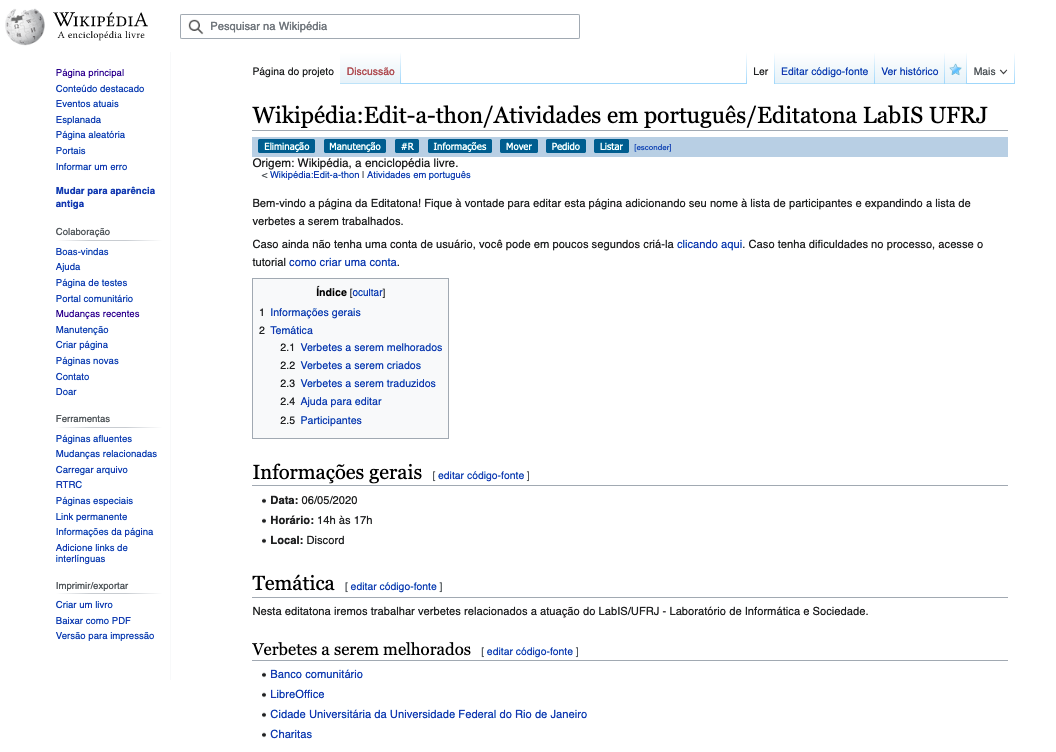
\includegraphics[width=1\textwidth]{Images/pagina_editatona.png}
    \caption{Página de organização de uma das editatonas realizadas durante a pesquisa com lista prévia de sugestões de verbetes a serem melhorados.}
    \label{fig:pagina_editatona}
\end{figure}

 Feita a discussão de quais temas serão trabalhados, o wikipedista experiente então edita o nome das salas que seguiam o padrão ``Grupo X'', adicionando em seus títulos quais temas serão trabalhados em cada sala. Os participantes são então convidados a clicarem no grupo que desejarem, e a sala ``Palestra de abertura'' é esvaziada.
 
 Neste momento começa de fato a escrita enciclopédica, e o wikipedista experiente passa a rodar entre os grupos para auxiliá-los. Para dar conta da escrita coletiva em computadores distintos, os grupos recebem a sugestão de utilizar a ferramenta Etherpad para escrita de seus rascunhos, antes das páginas de Testes da Wikipédia. O MediaWiki, software que gerencia a Wikipédia, não possui funcionalidades que apoiem a escrita ao vivo de textos por duas pessoas que estejam em máquinas diferentes. Isto não é um problema para editatonas presenciais, onde os novatos compartilham o mesmo teclado, mas para a atividade virtual seria muito desmobilizante pedir para um usuário esperar outro editar e salvar uma página de testes para somente então poder editar também.
 
O Etherpad é um software livre que oferece a possibilidade de usuários criarem simultaneamente textos online. Seu funcionamento guarda muitas similaridades com a ferramenta Google Docs, já amplamente conhecida por usuários da Internet. (ARRINGTON, 2008) Optamos por sugerir aos participantes das editatonas a utilização do Etherpad, e não da ferramenta da Google, por ele ser mais leve e não requerer autenticação dos usuários para editar.

Assim, o usuário experiente cria um pad (nome de uma página dentro do Etherpad) para cada grupo, e compartilha o link de cada um no chat de texto dentro do servidor do Discord de cada respectivo grupo.

\begin{figure}[H]
    \centering
    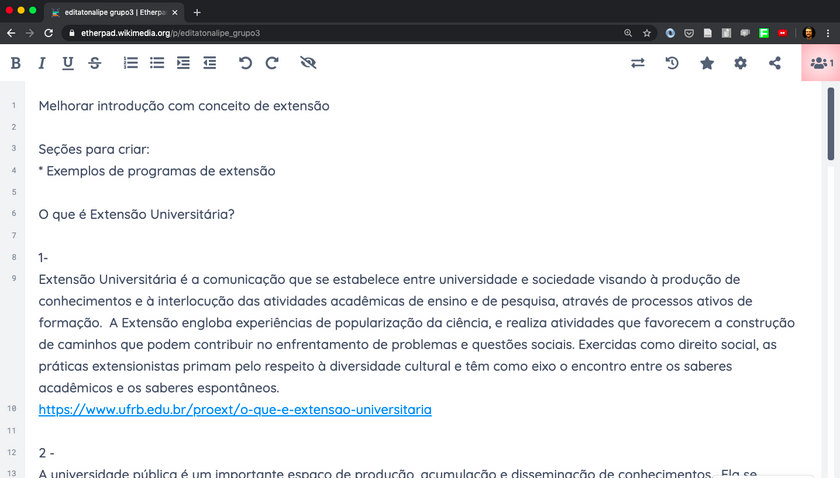
\includegraphics[width=1\textwidth]{Images/etherpad.png}
    \caption{Exemplo de um pad utilizando por um grupo durante uma editatona virtual.}
    \label{fig:etherpad}
\end{figure}

Os membros de cada grupo então são convidados a seguir o seguinte método: escrever no pad o rascunho do texto que irá para a Wikipédia e compartilhar no chat de texto do grupo no Discord links que possam ser utilizados como referências e demais conteúdos relacionados ao processo de escrita do grupo. Desta forma, além do trabalho do grupo ficar estruturado, participantes de demais grupos poderão acompanhar com facilidade o que estiver acontecendo no grupo, colaborando e até mudando de grupo com facilidade se desejarem.

\begin{figure}[H]
    \centering
    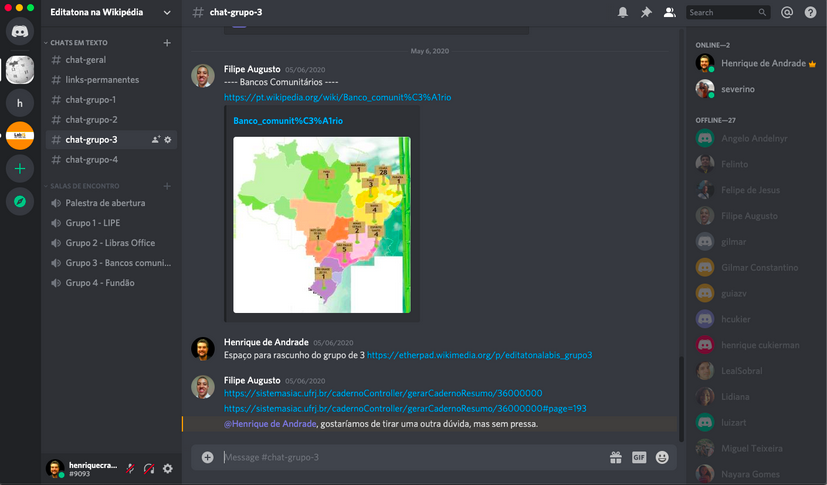
\includegraphics[width=1\textwidth]{Images/discord_full.png}
    \caption{Chat em texto de um grupo das editatonas virtuais, onde podem ser vistos o link para o pad sendo compartilhado e posteriormente um participante pedindo a presença do wikipedista experiente.}
    \label{fig:discord_chat}
\end{figure}

Após duas horas de produção de conteúdo, o wikipedista experiente roda todos os grupos uma última vez, os auxiliando a salvar seus conteúdos e convidando todos os participantes a retornarem para a sala "Palestra de abertura", onde é realizado um bate-papo final com todos, com cada grupo contando para os demais o que foi produzido, como foi a experiência e quais dificuldades encontraram no processo.

\subsection{Acompanhando as editatonas virtuais}

*** Ver https://trello.com/c/AzsF0ayG/450-reaproveitar-texto-sobre-contropedia-quando-come%C3%A7ar-a-apresentar-dados-das-minhas-editatonas

\subsubsection{Escolha dos grupos}

Para a realização, das editatonas foram convidados grupos próximos à linha de pesquisa de Informática e Sociedade da COPPE/UFRJ, que estivessem mobilizados virtualmente durante a pandemia, para editarem verbetes sobre seu assunto de interesse.

Esta escolha de convidados pode ser considerada um movimento de interessamento mútuo da pesquisa. Ao mesmo tempo que essas são redes já mobilizadas e com proximidade facilitante ao pesquisador que conduziu as atividades, os assuntos de interesse desses grupos seriam expandidos na enciclopédia são caros à linha de pesquisa onde este trabalho é realizado, tornando assim a escolha destes grupos para a realização das atividades um tanto quanto óbvia e oportuna.
 Foram então realizadas três editatonas virtuais com os seguintes coletivos da UFRJ: Laboratório de Informática e Sociedade (LabIS), Laboratório de Informática para Educação (LIpE) e Núcleo de Solidariedade Técnica (SOLTEC).
 
\subsubsection{Seguindo as Editatonas}

A primeira editatona com a metodologia virtual foi realizada com a equipe do Laboratório de Informática para Educação (LIpE), contando com a presença de 10 pessoas. Nesta atividade foram criados três grupos, focados em melhorar e escrever verbetes sobre as seguintes temáticas: "linguagem de programação Logo", "extensão universitária" e "história do LIpE".

Já a editatona realizada com o Laboratório de Informática e Sociedade (LabIS) teve a participação de 09 pessoas novas, além de dois membros do LIpE que haviam participado da primeira atividade e retornaram para seguir editando sobre a "história do LIpE". Assim, além do grupo que perdurou da atividade anterior, foram criados novos grupos para tratar dos temas "Libras Office", "bancos comunitários" e "Ilha do Fundão". Nesta atividade contamos com a participação de dois editores que haviam participado também de nossa atividade presencial com a turma de ECI em 2019.2, e puderam compartilhar valiosas comparações entre os dois modelos.

*** ….internet e máquina melhores que na UFRJ…. … mais cansativo de casa…

*** falar com Nayara e Rodrigo Palmeira e pegar mais declarações.

A terceira e última editatona virtual, realizada com o Núcleo de Solidariedade Técnica (SOLTEC), teve a participação de X pessoas e …..

A cada atividade realizada a metodologia de organização de editatonas virtuais sofreu alterações a partir do feedback dos participantes, com alterações inclusive na palestra de abertura.

*** atividade 1: principal feedback: terminar no horário. Um grupo também relatou que se atrapalhou quando cada um pegou uma parte do verbete para escrever separado, e melhorou quando se focaram todos na mesma seção de cada vez.

*** atividade 2: mais foco em edição na palestra de abertura.

*** narrar descoberta da "propaganda no Logo" e tentativa de interação pela PD.

*** narrar remoção do verbete sobre o Lipe.

*** Mostrar prints de verbetes

*** Números gerais. Pegar últimos parágrafos do arquivo estudosquantitativos.tex para justificar o uso de ferramentas quantitativas para análise das editatonas.

*** Apresentar quantos conteúdos de nossas editatonas ficaram no ar após X tempo.

*** Falar quantos acessos nossas edições tiveram, e qual a projeção de acessos em Y tempo.

*** Trazer fala de algum usuários específicos que tenham passado por alguma situação interessante para fechar.


%capítulo 4: afinando o instrumento
\chapter{Afinando o instrumento}

\singlespacing
\begin{flushright}

\textit{``Viver é afinar}

\textit{O instrumento...''}

Walter Franco
\end{flushright}
\doublespacing


%\backmatter

\printbibliography

\appendix

\end{document}